\makeatletter%stellare(~/Fisica-Stellare)
\let\@starttocorig\@starttoc
\makeatother%%

\documentclass[10pt,xcolor={usenames},fleqn]{beamer}

\usefonttheme{serif} % default family is serif

%% colors
\definecolor{bittersweet}{rgb}{1.0, 0.44, 0.37}
\definecolor{brilliantlavender}{rgb}{0.96, 0.73, 1.0}
\definecolor{antiquefuchsia}{rgb}{0.57, 0.36, 0.51}
\definecolor{violetw}{rgb}{0.93, 0.51, 0.93}
\definecolor{Veronica}{rgb}{0.63, 0.36, 0.94}
\definecolor{atomictangerine}{rgb}{1.0, 0.6, 0.4}
\definecolor{darkgray}{rgb}{0.66, 0.66, 0.66}
\definecolor{brightcerulean}{rgb}{0.11, 0.67, 0.84}
\definecolor{cadmiumorange}{rgb}{0.93, 0.53, 0.18}
\definecolor{ochre}{rgb}{0.8, 0.47, 0.13}
\definecolor{midnightblue}{rgb}{0.1, 0.1, 0.44}
\definecolor{lemon}{rgb}{1.0, 0.97, 0.0}
\definecolor{grey}{rgb}{0.7, 0.75, 0.71}
\definecolor{amber}{rgb}{1.0, 0.75, 0.0}
\definecolor{almond}{rgb}{0.94, 0.87, 0.8}
\definecolor{bf}{RGB}{88, 86, 88}
\definecolor{bb}{RGB}{177, 177, 177}
\definecolor{keyword}{rgb}{0.25, 0.25, 0.28}
\definecolor{todo}{rgb}{0.75, 0.0, 0.2}
\definecolor{must}{rgb}{1.0, 0.31, 0.0}

%beamer setup
\usepackage{beamersetup}

%%%%%%%%%%%%%%%%%%%%%%%%%%%%%%%%%%% importa pacchetti
\usepackage{usepkg}
%%%%%%%%%%%%%%%%%%%%%%%%%%%%%%%%%%% Funzioni generali
\usepackage{functions}
%http://tex.stackexchange.com/questions/246/when-should-i-use-input-vs-include
\newcommand{\setmuskip}[2]{#1=#2\relax} %%problem usinig mu with calc (req by mathtools) loaded

\usepackage{sources}


%\usepackage{length}
%%%%%%%%%%%%%%%%%%%%%%%%%%%%%%%%%%% Funzioni per questo file main
\usepackage{mathOp}

\def\status{coazione}%ripeter
\def\keeptrying{coazione}
\usepackage{LocalF}
%%%%%%%%%%%%%%%%%%%%%%%%%%%%%%%%%

\title{Fisica stellare}

% Let's get started
\begin{document}

\begin{filecontents}{conservedvector.tex}

\centering
\begin{figure}
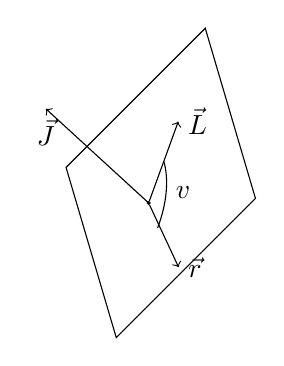
\begin{tikzpicture}[rotate around z=45, rotate around x=-45]
\draw (0,-0.3,0) -- (2.5,-0.3,0) -- (2.5,2.5,0) -- (0,2.5,0) -- cycle;
\draw[->] (1.,1.,0)node[draw,circle,inner sep=0] (o) {} -- (1.5,1.5,2)node[below] {$\vec{J}$};
\draw[->] (o) -- ++(295:0.9cm)node[right] {$\vec{r}$};
\draw[->] (o) -- ++(70:1.1cm)node[right] {$\vec{L}$}node [midway] (aux){};
\draw (aux) arc (0:-50:1) node[midway,right] {$v$};
\end{tikzpicture}

\label{fig:Lenztikz}

\end{figure}

\end{filecontents}%%contain tikz files as filecontents

\addtobeamertemplate{block begin}{\setlength\abovedisplayskip{2pt}\setlength\belowdisplayskip{2pt}\setlength\abovedisplayshortskip{2pt}\setlength\belowdisplayshortskip{2pt}}{}
\addtobeamertemplate{block begin}{\vspace*{-3pt}}{}
\addtobeamertemplate{block end}{}{\vspace*{-3pt}}

\begin{frame}
  \titlepage
\end{frame}

% Section and subsections will appear in the presentation overview
% and table of contents.
%\frame{\tableofcontents[onlyparts]}

\begin{frame}[label={argomenti}]{Fisica stellare: argomenti del corso}
\tableofcontents[onlyparts]
\end{frame}

\begin{wordonframe}{Meta.}
lbf, todo, keyword, must
\end{wordonframe}

\begin{wordonframe}{Perch\'e studio queste cose?? Sviluppi; futuro.}

Concretezza, concentrazione, indipendenza

\end{wordonframe}

\part{Intro}\linkdest{intro}
\section{Fonti}

\begin{wordonframe}{General}
Astrofisica stellare (castellani)
Rolfs rodney Couldron in the cosmos
iliadis nuclear burning
kippenhahn wiekert
salaris cassisi: evoluzione; popolazioni stellari;
\end{wordonframe}

\begin{wordonframe}{Milky way}
Thin disk thick disk transition
\end{wordonframe}

\begin{wordonframe}{popolazioni stellari}
salaris cassisi ch 9, 10, 11
\end{wordonframe}



\section{RegLez 19}\linkdest{reglez}
\begin{frame}[allowframebreaks]{Reg Lez 19}
\begin{itemize}
\phantomsection\linkdest{febbraio}
\item 18/02/2019 - Descrizione del corso. Descrizione generale della via Lattea. Definizione di ammasso stellare. Ammassi aperti ed ammassi globulari. Caratteristiche generali delle stelle di disco e di alone. Richiami alle definizioni di magnitudine, indice di colore, modulo di distanza. Cenni alla curva universale delle abbondanze (nel disco galattico). Alpha enhancement.  
\item 19/02/2019 - Caratteristiche generali del bulge e del thick disk. Discussione dell'origine dell'alpha enhancement. Scenario qualitativo generale della formazione della nostra Galassia. Alone interno ed alone esterno e relazione con la cattura di galassie nane durante la formazione della Galassia. Cenni alla formazione inside out del disco. Generalità su diagrammi colore- magnitudine di disco e di campo. Present day mass function ed initial mass function. Relazione massa-luminosit\'a. 
\item 22/02/2019 - Cenni alla derivazione dello Star formation rate e della relazione massa-luminosit\'a per il disco della nostra Galassia. Cenni alla produzione di elementi nella nucleosintesi primordiale. Generalit\'a sui metodi di determinazione delle abbondanze chimiche nel sistema solare. 
\item 25/02/2019 - Discussione del problema della determinazione dell'elio primordiale e dell'elio in stelle di disco. Cenni alla struttura del gruppo locale ed alle caratteristiche delle popolazioni stellari all'interno delle galassie del Gruppo Locale. Discussione del problema della multipopolazione negli ammassi globulari. 
\item 26/02/2019 - Generalit\'a su strutture autogravitanti. Stima del tempo scala dinamico. Richiamo al tempo di free fall. Equazioni di equilibrio stellare: equilibrio idrostatico ed equazione di continuit\'a. Peso molecolare medio. Esempio: calcolo del peso molecolare medio per materia completamente ionizzata. Peso molecolare medio degli ioni. Peso molecolare medio per elettrone. Generalit\'a sull'equazione del trasporto radiativo e sull'opacit\'a. Dimostrazione per ordini di grandezza che la presenza di un flusso negli interni stellari non contraddice l'assunzione di equilibrio termodinamico. 
\phantomsection\linkdest{marzo}
\item 01/03/2019 - Equilibrio termico per le stelle. Stima del tempo scala termico. Equazione dell'equilibrio termico (di conservazione dell'energia). Energia persa per neutrini; cenni ai processi principali. Calcolo della produzione di energia gravitazionale; problema della stima dell'energia gravitazionale del "primo modello" calcolato. 
\item 04/03/2019 - Integrazione delle equazioni di equilibrio stellare: interno, subatmosfera ed atmosfera. Cenni ai metodi di integrazione dell'atmosfera (variabile indipendente profondit\'a ottica). Metodo iterativo per il calcolo delle variabili fisiche esterne in atmosfera. Cenni al problema della determinazione della pressione di turbolenza e del gradiente ambientale nelle zone convettive esterne. Metodi numerici di integrazione delle equazioni di equilibrio stellare: il metodo del fitting. 
\item 05/03/2019 - Metodo di Henyey per l'integrazione delle equazioni di equilibrio stellare. Relazione tra energia termica ed energia gravitazionale in una struttura stellare all'equilibrio idrostatico. Il teorema del viriale per le strutture stellari: gas perfetto monoatomico e non monoatomico. Criterio di stabilit\'a per le strutture stellari in base al valore della costante adiabatica del gas. Relazioni per ordini di grandezza tra quantit\'a fisiche in strutture stellari ricavate utilizzando le equazioni di equilibrio stellare ed il teorema del viriale: relazione tra massa, densit\'a e temperatura, relazione tra luminosit\'a, massa, peso molecolare medio ed opacit\'a. 
\item 08/03/2019 - Approssimazione di strutture stellari a politropiche. Equazione di Lane-Emden e modalit\'a di risoluzione. Cenni a strutture isoterme. Esempio. il modello solare approssimato con una politropica. 
\item 11/03/2019 Equazione del trasporto radiativo. Generalit\'a sul trasporto di energia tramite conduzione elettronica. Coefficiente di diffusione per conduzione. Definizione dell'"opacità di conduzione" e sua stima approssimata nel gaso di gas degenere non relativistico. Generalit\'a su calcolo dell'opacit\'a radiativa. Calcolo dell'opacit\'a (in forma analitica) per: scattering elettronico, processi free free, fotoionizzazione. Opacit\'a nelle atmosfere stellari: opacit\'a di interazione fotoni-ione H- . 
\item 12/03/2019 - L'equazione di stato delle strutture stellari. Gas degenere elettronicamente. Effetti coulombiani nelle strutture stellari. Equazione di Saha.
\item  15/03/2019 - La media di Rosseland dell'opacità sulla distribuzione in frequenza dei fotoni. Discussione di grafici relativi all'andamento dell'opacit\'a negli interni stellari. Criterio di Schwarzschild per l'innesco della convezione. Cenni al problema dell'overshooting.
\item 18/03/2019 - Criterio di Ledoux per l'innesco della convezione nel caso di gas perfetto e non. Relazioni tra gradiente radiativo, ambientale ed adiabatico. Il gradiente ambientale negli interni e negli esterni stellari. Metodo della mixing length per il trattamento della convezione negli esterni stellari: Calcolo approssimato dell'altezza di scala della pressione, calcolo del flusso convettivo e del gradiente ambientale, in funzione della velocità media degli elementi di convezione.
\item 19/03/2019 - Teoria della mixing length per il calcolo del flusso convettivo: calcolo della velocità media degli elementi di convezione. Meccanismi di fusione nucleare nelle stelle. Sezione d'urto di fusione tra particelle cariche ed espressione per il rate di fusione nucleare. Picco di Gamow. Calcolo approssimato dei rates di fusione nucleare tra particelle cariche. Dipendenza approssimata delle reazioni nucleari tra particelle cariche dalla temperatura.
\item 22/03/2019 - Esempi di misure di sezioni d'urto nucleari. Sezione d'urto risonante: risonanze strette. Lo schermaggio elettronico in laboratorio. Calcolo approssimato dell'effetto di schermaggio elettronico in laboratorio. Lo schermaggio elettronico del plasma stellare: schermaggio debole e forte.
\item 25/03/2019 - Schermaggio elettronico nelle stelle. Calcolo dell'effetto di schermaggio debole. Correzione al rate di fusione dovuto alla presenza di schermaggio debole. Reazioni di fusione di elementi leggeri: deuterio, litio, berillio e boro. Fusione di idrogeno in elio: generalità e calcolo approssimato del flusso di neutrini solari. Reazione protone-protone: calcolo del tempo scala di fusione dei protoni nel Sole. Elementi primari ed elementi secondari in una catena di reazioni. Abbondanza di equilibrio degli elementi secondari. Esempio: calcolo dell' abbondanza di equilibrio del deuterio. Raggiungimento dell'abbondanza di equilibrio dell'elio 3 nella catena protone protone.
\item 26/03/2019 - Il bi-ciclo CN-NO: caratteristiche generali. Cenni allo spetto di neutrini solari. Cicli di CNO veloce. Dipendenza dalla temperatura della catena pp e del bi-ciclo CN-NO. Cenni alla caratteristiche delle stelle di sequenza principale inferiore e superiore dovute alle modalit\'a di combustione di H in He. Reazione 3 alfa per la fusione di elio in 12C e 12C+alfa per la produzione di 16 O. Confronto 12C + alfa e 16O + alfa alle condizioni fisiche tipiche della fusione di elio al centro.
\item 29/03/2019 - Influenza della sezione d'urto 12C + alfa sul tempo di vita in fase di combustione di elio centrale. Catene di produzioni di neutroni liberi. Reazioni in fasi evolutive avanzate: fusione di 12C, fotodisintegrazione del 20Ne, fusione dell'16O , fotosintegrazione del 28Si, catene di catture alfa su nuclei fino alla produzione di 56Fe.
\phantomsection\linkdest{aprile}
\item 01/04/2019 - Catture neutroniche su nuclei: andamento della sezione d'urto con l'energia e con il peso atomico. Processi s e processi r. Tempo di vita di un nucleo per cattura neutronica. Stima del flusso di neutroni caratteristico di processi s ed r. Stima dell'abbondanza di equilibrio per processi s. Spiegazione qualitativa dell'andamento dei picchi "s" ed "r" nella curva universale delle abbondanze. Cenni alle caratteristiche di protostella ed al passaggio tra protostella e stella di Pre-Sequenza Principale.
\item 02/04/2019 - Lezione seminariale del dott. Emanuele Tognelli su formazione stellare: tempo di Kelvin-Helmholtz, accrescimento della protostella fino al primo ed al secondo core idrostatico. Evoluzione di PMS: traccia di Hayashi.
\item 05/04/2019 - Lezione seminariale del dott. Tognelli su: evoluzione di Pre-Sequenza Principale. Ruolo dell'opacità dell'H- nella verticalit\'a della traccia di Hayashi, innesco della fusione del deuterio. Stelle completamente convettive. Stelle che in PMS sviluppano un nucleo radiativo.
\item 08/04/2019 - Zero Age Main Sequence. Approccio alla ZAMS per stelle di sequenza principale inferiore e superiore. Il profilo di abbondanza di equilibrio dell'3He. Caratteristiche generali delle stelle di sequenza principale inferiore e superiore. Dipendenza della posizione della ZAMS nel diagramma HR dall'abbondanza originale di elio e metalli. Accenno al metodo di determinazione di DY/DZ dal confronto teoria-osservazione per stelle di disco locale parallassate, Dipendenza della massa di transizione dall'abbondanza originale di elio e metalli. Massa minima e massima in ZAMS.
\item 09/04/2019 - Influenza sulla posizione della ZAMS del diagramma HR delle incertezze negli input fisici utilizzati dai modelli e nell'efficienza della convezione esterna. Metodo del Main Sequenze fitting per la determinazione della distanza di ammassi, criticit\'a del metodo. Evoluzione di sequenza principale per stelle di sequenza principale inferiore e superiore. Modalit\'a di esaurimento dell'H centrale per stelle di sequenza principale inferiore e superiore: Turn Off and Overall Contraction. Fase di subgigante rossa (SGB). Gap di Hertzsprung.
\item 12/04/2019 - Dalla fase di subgigante a quella di gigante rossa. Tracce evolutive ed isocrone di ammasso. Il Turn Off/Overall Contraction come indicatore di et\'a. Isocrone di ammassi giovani e vecchi. Evoluzione di gigante rossa: il primo dredge up.
\item 15/04/2019 - Morfologia del ramo delle giganti rosse per stelle di massa piccola ed intermedia: massa di "RGB transition". Dipendenza della massa di RGB transition dalla composizione chimica. Massa del nucleo di elio all'innesco dell'elio centrale in funzione della massa totale della stella. Luminosit\'a del vertice del ramo delle giganti rosse (RGB tip) in funzione della massa totale della stella. Dipendenza della massa del nucleo di elio all'innesco e della luminosità di RGB tip dalla composizione chimica. Dipendenza dell'isocrona e della luminosit\'a del TO/OC dall'abbondanza originale di elio e metalli. Influenza sull'isocrona e sulla luminosit\'a del TO della diffusione microscopica. Il bump dell'RGB. Dipendenza della luminosit\'a del bump dall'efficienza della convezione esterna, dall'et\'a dell'ammasso e dalla composizione chimica. Il tip dell'RGB come indicatore di distanza. Dipendenza della luminosit\'a del tip dalla composizione chimica. Innesco dell'elio a flash per stelle di piccola massa.
\item 16/04/2019 - Stelle in combustione centrale di elio: la ZAHB. Caratteristiche generali degli hot flashers. Il ramo orizzontale anomalo in ammassi stellari giovani a bassa metallicit\'a in galassie esterne: l'RGB clump. La Zero Age Horizontal Branch come indicatore di distanza. Dipendenza della luminosit\'a della ZAHB dalla composizione chimica. Cenni al metodo orizzontale per la determinazione dell'et\'a di ammassi antichi. Il metodo verticale per la determinazione dell'et\'a di ammassi antichi. Cenni alla discrepanza teoria-osservazione per la luminosit\'a del bump dell'RGB.
\item 29/04/2019 - Evoluzione in combustione di elio per stelle di ramo orizzontale. Combustione di elio centrale per stelle di massa intermedia; il clump dell'elio in ammassi di et\'a intermedia. Il clump dell'elio come indicatore di distanza. Combustione di elio centrale per stelle di massa intermedia-grande; il loop dell'elio. Incertezza nella determinazione di et\'a di ammassi antichi tramite il metodo verticale.
\item 30/04/2019 - Effetto dell'overshooting sui modelli di sequenza principale superiore e sulla determinazione di et\'a di ammassi di et\'a giovane-intermedia. Incertezze sulla determinazione di et\'a di ammassi di et\'a giovane-intermedia. Discussione sui parametri che influenzano la morfologia di ramo orizzontale.
\phantomsection\linkdest{maggio}
\item 03/05/2019 - Effetto della presenza di diffusione microscopica sulla determinazione dell'et\'a tramite il metodo verticale. Il parametro R per la determinazione dell'elio. Esaurimento dell'elio centrale: autotrascinamento del nucleo, semiconvezione e pulsi convettivi.
\item 06/05/2019 - Ingresso in fase di ramo asintotico: il clump dell'AGB. AGB manque'. Evoluzione di ramo asintotico: il secondo dredge-up. Pulsi termici e terzo dredge-up. Nucleosintesi di elementi s in AGB: la tasca di 13C. Produzione di litio in AGB.

\item 07/05/2019 - Lezione seminariale del dott. Emanuele Tognelli su: abbondanza superficiale di elementi leggeri in fase di Pre-Sequenza Principale. Il metodo del "lithium depletion boundary" per la datazione di ammassi giovani.
\item 10/05/2019 - Caratteristiche generali dell'evoluzione avanzata di stelle massicce. Destino finale di stelle di varia massa: nane bianche di He, C/O, O/Ne, supernovae di tipo II da deflagrazione del carbonio e da cattura elettronica su nuclei, supernovae di tipo II da fotodisintegrazione del ferro.
\item 13/05/2019 - lezione: Discussione sul 60Fe come elemento indicatore di esplosioni di supernova nelle vicinanze della Terra negli ultimi milioni di anni. Supernovae di tipo II: caratteristiche di pre-supernova. Emissione di neutrini e loro interazione con i nuclei del nocciolo denso della supernova. Intrappolamentp e temposcala di emissione dei neutrini. Stima per ordini di grandezza dell'energia emessa sotto varie forme (neutrini, fotoni, energia del fronte di shock). Neutronizzazione esplosiva e meccanismo di esplosione ritardata. Discussione sulle caratteristiche della supernova 1987A, sul flusso di neutrino osservato e sulla sua osservazione in varie bande elettromagnetiche nelle varie fasi di supernova.. Classificazione dei vari tipi di supernovae in base allo spettro ed alla morfologia della curva di luce.
\item 14/05/2019 - Lezione seminariale del prof. Prada Moroni su evoluzione delle nane bianche.
\item 17/05/2019 - Caratteristiche e metodo di calcolo del modello solare standard. Generalita' sull'eliosismologia e sui modelli solari eliosismologici. Generalità sulla rivelazione dei neutrini solari come test aggiuntivo del modello solare standard.
\item 20/05/2019 - Stelle variabili pulsanti: cenni al meccanismo di pulsazione. La striscia di instabilita' nel diagramma HR ed i vati tipi di stelle variabili pulsanti. RR Lyrae: diagramma di Bailey, curve di luce, relazione periodo, luminosita', massa e temperatura effettiva. Le RR Lyrae come indicatori di distanza. Il parametro A come indicatore di elio. Stelle cefeidi classiche. Uso delle stelle cefeidi come indicatori di distanza di ammasso e di campo. La dicotomia di Oosterhoff.
\item 21/05/2019 - Lezione seminariale del dott. Cignoni su studi di popolazione nella galassie esterne: recupero della star formation history. Analisi di popolazioni non risolte semplici e complesse.
\item 24/05/2019 - lezione: Caratteristiche generali delle SNIa. Possibili progenitori della SNIa: generalità su meccanismi di scambio di massa in sistemi binari, sistemi finali dopo due common envelope, possibili scenari di accrescimento di H/He/C su una compagna degenere. La SNIa come indicatori di distanza.
\end{itemize}
\end{frame}

\section{RegLez 17}

\begin{frame}[allowframebreaks]{Reg Lez 17}
\begin{itemize}
\item testo: Popolazioni stellari: formazione stellare (fenomenologia)
\item lezione: Descrizione generale della struttura della nostra Galassia. Concetti base: parallasse, magnitudine assoluta ed apparente, modulo di distanza, estinzione ed arrossamento. Caratteristiche generali di ammassi aperti e globulari. Alpha enhancement.
\item lezione: Caratteristiche fotometriche, dinamiche e chimiche delle popolazioni stellari della nostra Galassia. Caratteristiche generali delle stelle di thick disk. Relazione massa-luminosit\'a per le stelle di sequenza principale. Relazione generale tra massa e tempo di vita di una stella. Initial Mass Function and Present Day Mass Function.
\item lezione: Differenze generali tra stelle di ammasso e stelle di campo. Esempi di diagrammi Colore-Magnitudine di stelle di ammasso e stelle di campo. Discussione generale sullo studio delle caratetristiche delle stelle di campo. Cenni alla determinazione dello ''Star Formation Rate'' per il disco della nostra Galassia ed alla determinazione della relazione et\'a-metallicit\'a. 
\item lezione: Scenario generale di formazione della Via Lattea. Cenni alle galassie del Gruppo Locale. Cenni alle popolazioni stellari nella Via Lattea e nella galassie del Gruppo Locale. Metodi di determinazione delle abbondanze stellari. La curva ''universale'' delle abbondanze. Cenni alla nucleosintesi primordiale.
\item lezione: Discussione generale sulla multipopolazione negli ammassi globulari della nostra Galassia. 
\item Testo: Equazioni struttura stellare: fenomenologia e metodi numerici
\item lezione: Equilibrio idrostatico nelle stelle. Equazioni di equilibrio stellare: equilibrio idrostatico ed equazione di continuit\'a.
\item lezione: Peso molecolare medio. Esempio: calcolo del peso molecolare medio per materia completamente ionizzata. Peso molecolare medio degli ioni. Peso molecolare medio per elettrone. Generalit\'a sull'equazione del trasporto radiativo. Equilibrio termico. Le equazioni di equilibrio stellare. Calcolo dell'energia "gravitazionale".
\item lezione: Calcolo approssimato del tempo scala termico nell'interno del Sole. L'equazione del trasporto nelle atmosfere stellari. Profondit\'a ottica. Equazioni di equilibrio stellare in atmosfera. Generalit\'a sui metodi numerici di integrazione delle equazioni di equilibrio stellare. Il metodo del fitting.
\item lezione: Seminario del dott. Tognelli su: l'equazione di stato delle strutture stellari. Gas degenere elettronicamente. Effetti coulombiani nelle strutture stellari. Equazione di Saha.
\item lezione: Il metodo di Henyey per la risoluzione delle equazioni di equilibrio stellare. Integrazione dell'atmosfera. L'equazione del trasposto radiativo. Il teorema del viriale per le strutture stellari: caso di gas perfetto monoatomico. Tempo scala di Kelvin-Helmholtz.
\item lezione: Il teorema del viriale: gas perfetto non monoatomico. Criterio di stabilit\'a delle strutture stellari. Utilizzo delle equazioni di equilibrio stellare e del teorema del viriale per ottenere relazioni per ordini di grandezza tra: 1) massa, densit\'a e temperatura delle stelle 2) massa-luminosit\'a.
\item lezione: Calcolo approssimato dell'opacit\'a da scattering Thompson nel caso di ionizzazione totale. Formula di Kramer per opacit\'a free-free e bound free. Opacit\'a legata agli ioni H-.
\item lezione: La conduzione elettronica. Opacit\'a conduttiva. Equazione del trasporto in presenza di opacit\'a conduttiva. Criterio di Schwarzschild e di Ledoux per l'innesco della convezione in ambiente stellare. Cenni al fenomeno dell'overshooting.
\item lezione: Il metodo della mixing lenght per il trattamento della convezione negli inviluppi esterni stellari. Calcolo approssimato dell'altezza di scala della pressione. 
\item lezione: La teoria della mixing lenght per il trattamento della convezione negli esterni stellari: calcolo del flusso convettivo, della velocit\'a media delle bolle di convezione e del gradiente ambientale negli esterni stellari. Modelli politropici di strutture stellari: equazione di Lane-Emden e calcolo dell'andamento di pressione e densit\'a per modelli stellari politropici. Esempi: il modello solare.
\item Testo: Produzione enrgia: reazioni nucleari (evoluzione)
\item lezione: Calcolo dei rates di reazioni di fusione nucleare tra particelle cariche. La probabilit\'a di penetrazione della barriera coulombiana ed il fattore astrofisico. Il picco di Gamow. Espressione approssimata dei rates di fusione nucleare. Dipendenza approssimata delle reazioni dalla temperatura.
\item lezione: Lo schermaggio elettronico in laboratorio. Lo schermaggio elettronico nel plasma stellare: schermaggio debole, intermedio e forte. Trattamento dello schermaggio debole negli interni stellari secondo il metodo di Salpeter. 
\item lezione: Reazioni nucleari di combustione di elementi leggeri. Elementi primari ed elementi secondari. Concentrazione di equilibrio per gli elementi secondari. Reazioni di fusione di H in He: la catena protone-protone ed il bi-clo CN-NO. Neutrini solari.
\item lezione: Reazioni del ciclo CNO veloce. Reazioni di fusione di elio in C ed O. Catene di produzione di neutrini liberi in fasi evolutive avanzate.
\item lezione: Reazioni di fusione del C e dell'O. Reazioni nucleari successive fino alla produzione degli elementi del picco del ferro. Struttura a cipolla di pre-supernova e nucleosintesi esplosiva. Catture neutroniche su nuclei: processi s e processi r. Sezione d'urto per cattura neutronica ed andamento con l'energia del rate delle reazioni di cattura neutronica. Stima del flusso di neutroni caratteristico di processi s ed r. Stima dell'abbondanza di equilibrio per processi s. Spiegazione qualitativa dell'andamento dei picchi "s" ed "r" nella curva universale delle abbondanze.
\item Testo: MS-PMS
\item lezione: Seminario del dott. Emanuele Tognelli su caratteristiche delle fasi di protostella e di Pre-Sequenza Principale (PMS). Traccia di Hayashi. Effetto di variazione di massa e composizione chimica in PMS. Combustione del deuterio ed effetti sulle strutture di PMS.
\item lezione: Caratteristiche e metodo di calcolo del solare standard. Generalit\'a sull'eliosismologia e sui modelli solari eliosismologici.
\item lezione: Seminario del dott. Tognelli su evoluzione di Pre-sequenza principale, evoluzione temporale dell'abbondanza superficiale di elementi leggeri. Ingresso in ZAMS per stelle di sequenza principale inferiore e superiore.
\item lezione: Dipendenza della posizione di PMS nel diagramma HR dalla composizione chimica e dall'efficienza della convezione esterna. Zero Age Main Sequence. Dipendenza della posizione di ZAMS nel diagramma HR dalla composizione chimica e dall'efficienza della convezione esterna. Stelle di sequenza principale inferiore e superiore. Approccio alla ZAMS: sviluppo di un piccolo nucleo convettivo per stelle di SPI durante il raggiungimento dell'abbondanza di equilibrio dell'3He. Profilo dell'abbondanza di equilibrio dell'3He per stelle di SPI.Very low mass. Calcolo approssimativo della massa minima per l'innesco della fusione di H in He. 
\item lezione: Evoluzione di sequenza principale. Modalit\'a di esaurimento dell'idrogeno centrale per stelle di sequenza principale inferiore e superiore. Fase di subgigante rossa. Isocrona di ammasso. La luminosit\'a all'esaurimento dell'idrogeno centrale come indicatore di et\'a di una popolazioen stellare semplice. 
\item lezione: Incertezze nelle previsioni teoriche di MS. Generalit\'a sulle isocrone di ammasso. Il metodo del fitting della MS per la determinazione della disatnza degli ammassi globulari. La luminosit\'a del TO/OC come indicatore di et\'a. Evoluzione di sub-gigante rossa. Dipendenza delle tracce di MS/SGB dalla composizione chimica. Influenza della diffusione sulla traccia di stelle di data massa nel diagramma HR.
\item Testo: Post Hydrogen
\item lezione: Evoluzione di gigante rossa: il primo dredge up ed il bump dell'RGB. Dipendenza della luminosit\'a del bump dalla composizione chimica. Perdite di massa in RGB. Il flash dell'elio. Morfologia dell'RGB per ammassi stellari giovani ed antichi.
\item lezione: Massa dell'elio all'innesco dell'elio centrale in funzione della massa totale della stella. Massa di RGB transition e sua dipendenza dalla composizione chimica. Dipendenza della luminosit\'a del vertice del ramo della giganti rosse dalla composizione chimica. Il tip dell'RGB come indicatore di distanza.
\item lezione: Dipendenza dell'isocrona dalla composizione chimica e dalla diffusione. Fase di combustione di elio per stelle di ammasso antico: il ramo orizzontale, HB. Zero Age Horizontal Branch. Il ramo orizzontale come candela campione, metodo verticale per la determinazione dell'et\'a di ammassi antichi. Dipendenza della ZAHB dalla composizione chimica.
\item lezione: Influenza della diffusione sulla determinazione dell'et\'a degli ammassi tramite il metodo verticale. Evoluzione di ramo orizzontale. Morfologia del ramo orizzontale: dipendenza da metallicit\'a ed et\'a dell'ammasso. Hot flashers. Il clump dell'elio ed il loop dell'elio. Il clump dell'elio come indicatore di distanza.
\item lezione: Effetto della presenza di overshooting sulla determinazione di et\'a di ammassi giovani. Discussione dell'incertezza sulla detrminazione di et\'a in ammassi stellari. Evoluzione in combustione di elio centrale: autotrascinamento e semiconvezione. Il parametro R per la stima dell'abbondanza di elio in ammassi antichi.
\item lezione: Cenni su stelle variabili come indicatori di distanza: RR Lyrae e cefeidi classiche. Ingresso in ramo asintotico. Il clump dell'AGB in stelle di piccola massa. Caratteristiche generali per stelle di AGB. Il secondo dredge up. Nucleosintesi in AGB. Pulsi termici.
\item lezione: Evoluzione della luminosit\'a durante i pulsi termici. Terzo dredge up, hot bottom burning. Catene di produzione di neutroni liberi e processi s in fase di ramo asintotico.
\item lezione: Evoluzione finale di stelle di varia massa. Nane bianche di C/O e O/Ne, supernovae di tipo II da deflagrazione del carbonio e da cattura elettronica su nuclei. Supernovae di tipo II da fotodisintegrazioen del ferro.
\item Lezione seminariale del prof. Prada Moroni su caratteristiche strutturali delle nane bianche, curva di raffreddamento di nana bianca. Misura di distanza ed et\'a in ammasso tramite la curva di raffreddamento delle nane bianche.
\item lezione: Lezione seminariale del prof. Cignoni su popolazioni stellari complesse nelle vicinanze del Sole e nelle galassie nane. recupero della star formation rate in popolazioni complesse.
\end{itemize}
\end{frame}
\section{Succo}\linkdest{succo}

\begin{frame}{* formation}
	contenu...
\end{frame}

\begin{frame}[fragile]{Struttura di equilibrio}\frameintoc
\begin{itemize}
\item Equilibrio idrostatico: pressione in un mesh \'e il peso della materia sopra per unit\'a di superficie. Stabilit\'a e tempi reazione a perturbazione
\item Pressione radiativa. Una frazione $\kappa$ del flusso di momento $\frac{F}{c}$ \'e assorbita dalla materia (momentum transfer per $cm^3$ per sec): $dq=-(n_{\nu}\,dSc\,dt)*(\kappa\rho\,dr)*\frac{h\nu}{c}$, il primo termine \'e il numero di fotoni pasanti per superficie $dS$ in tempo $dt$, il secondo \'e la probabilit\'a d'assorbimento attraverso spessore $dr$, il terzo \'e la quantit\'a di moto di ogni fotone.
\begin{align*}
&dP_r=\TDy{S}{F}=\TDof{S}\TDy{t}{q}=-\int \,d\nu n_{\nu}c\kappa_{\nu}\rho\,dr\frac{h\nu}{c}\\
&F_{\nu}=n_{\nu}ch\nu,\ \TDy{r}{P(Rad)}=-\int\,d\nu\frac{F(Rad)}{c}\kappa_{\nu}\rho
\end{align*}
\begin{comment}
Un elemento di volume $dS\,dr$ subisce per effetto dell'assorbimento della radiazione una variazione d'impulso $dq$, nel caso un fotone venga assorbito la variazione del flusso uscente \'e $dF<0$
The distribution of photons over over different quantum states with energies $\epsilon_k=\hbar\omega_k$ (large volume $\omega_k\to\omega$) 
\begin{align*}
\overline{n_k}=\frac{1}{\exp{\frac{\hbar\omega}{KT}}-1}
\end{align*}
Moltiplicando il numero di stati nel dato range di frequenze per la distribuzione di Plank (numero di occupazione) ottengo il numero di fotoni e l'energia radiativa nel range di frequenza
\begin{align*}
&dN_{\omega}=\frac{V}{\pi^2c^3}\frac{\omega^2\,d\omega}{\exp{\frac{\hbar\omega}{KT}}-1}\\
&dE_{\omega}=\frac{V\hbar}{\pi^2c^3}\frac{\omega^3\,d\omega}{\exp{\frac{\hbar\omega}{KT}}-1}
\end{align*}
\end{comment}
\end{itemize}
\end{frame}

\begin{frame}{Rotazione, mass loss}
\begin{itemize}
\item Rotazione. \[\frac{\nabla P}{\rho}=-\nabla\phi+\vec{a}=-\nabla\phi+\Omega^2r_{\perp}=\vec{g}_{eff}\]
If $\nabla\wedge(\Omega^2r_{\perp})=0$: $\phi\to\phi-V$, $V=\int_0^{r_{\perp}}\Omega^2r_{\perp}\,dr_{\perp}$ (OK if $P(\rho)$, politrope, regioni convettive)
\end{itemize}
\end{frame}

\begin{frame}{Stability}

\end{frame}

\begin{frame}{Hayashi Line (HL)}

\end{frame}

\part{Modelli stellari: struttura ed evoluzione}\linkdest{evolutivemodels}
\begin{frame}{this part toc}
\begin{itemize}
\item Tempi scala
\end{itemize}
\end{frame}
\section{Equazioni struttura stellare}\linkdest{stellarmodel}

\begin{wordonframe}{da fare: kippenhahn wiegert}
\begin{itemize}
\item strutture autogravitanti 1-62' (43). EQuilibrio idrostatico, vento stellare, stabilit\'a e pulsazioni
\item metodi numerici 77'-84(44-48)
\item esistenza e unicit\'a 85'-99'(48-56)
\item Properties of stellar matter: ideal gas with radiation, ionization, degenerate electron gas, equazione di stato, opacit\'a 102'-144'(57-78)
\item produzione energia reazioni nucleari:  146'-172'(79-92)
\item politrope 174'-190' (93-102)
\end{itemize}
\end{wordonframe}

\subsection{Struttura di equilibrio}\linkdest{stellarstructure}

\begin{frame}{Equazioni struttura di equilibrio}

\begin{align*}
&\TDy{m}{r}=\frac{1}{4\pi r^2\rho}\\
&\TDy{m}{P}=-\frac{Gm}{4\pi r^4}\overbrace{[-\frac{1}{4\pi r^2}\PtwoDy{t}{r}]}^{\tau_{hyd}=\frac{1}{2}(G\exv{\rho})\expy{-1/2}}\\
&\TDy{m}{T}=-\nabla\frac{T}{p}\frac{Gm}{4\pi r^4}\\
&\TDy{m}{L}=\epsilon-\epsilon_{\nu} \underbrace{-c_P[\TDy{t}{T}-\nad\frac{T}{P}\TDy{t}{P}]}_{-c_P\PDy{t}{T}+\frac{\delta}{\rho}\PDy{t}{P}}\\
&\TDy{t}{X_s}\frac{1}{A_s}=\sum_{production}\rho^{n_h+n_k-1}n_p\frac{X_h^{n_h}X_k^{n_k}}{A_h^{n_h}A_k^{n_k}}\frac{\exv{\sigma v}_{hk}}{m_H^{n_h+n_k-1}n_h!n_k!}\\
&-\sum_{distruction}\rho^{n_d+n_j-1}n_d\frac{X_s^{n_d}X_j^{n_j}}{A_s^{n_d}A_j^{n_j}}\frac{\exv{\sigma v}_{sj}}{m_H^{n_d+n_j-1}n_d!n_j!}
\end{align*}
\end{frame}

\begin{frame}{Conservazione massa e HE}
\begin{columns}[T]
	\begin{column}{0.5\textwidth}
\begin{align*}
&\TDy{m}{r}=\frac{1}{4\pi r^2\rho}\\
&\TDy{m}{P}=-\frac{Gm}{4\pi r^4}\overbrace{[-\frac{1}{4\pi r^2}\PtwoDy{t}{r}]}^{\tau_{hyd}=\frac{1}{2}(G\exv{\rho})\expy{-1/2}}\\
&\tau_{hyd}=\sqrt{\frac{R^3}{GM}}
\end{align*}
\end{column}\begin{column}{0.5\textwidth}
\begin{align*}
&\TDy{r}{m}=4\pi r^2\rho\\
&\TDy{r}{P}=-\frac{Gm}{r^2}\rho\overbrace{[-\rho\PtwoDy{t}{r}]}^{\tau_{hyd}=\frac{1}{2}(G\exv{\rho})\expy{-1/2}}\\
&\tau_{ff}=\sqrt{\frac{R}{g}}\\
&\tau_{exp}=R\sqrt{\frac{\rho}{P}}
\end{align*}
\end{column}
\end{columns}
Red giant: $\tau_H\approx\SI{5}{\day}$ (time for the shock to cross a supergiant star making a SNII, Cepheid); Sun: $\tau_H\approx\SI{38}{\minute}$; WD: $\tau_H\approx\SI{2}{\second}$
\end{frame}

\begin{frame}{Trasporto energia verso la superficie e gradiente termico}
\begin{columns}[T]
	\begin{column}{0.6\textwidth}
		\begin{align*}
		&\TDy{m}{T}=-\nabla\frac{T}{p}\frac{Gm}{4\pi r^4}\\
		&\nabla=\nrad=\frac{3\kappa_R}{16\pi acG}\frac{LP}{mT^4}\tag*{$\nrad\leq\nad$}\\
		&\nabla=\nad+\Delta\nabla\tag*{$\nrad>\nad-\frac{\chi_{\mu}}{\chi_T}\nmu$}
		\end{align*}
	\end{column}\begin{column}{0.4\textwidth}
		\begin{align*}
		&\TDy{r}{T}=\nabla\frac{T}{p}\TDy{r}{p}\\
		&\nabla=\TDly{P}{T}
		\end{align*}
	\end{column}
\end{columns}
\begin{align*}
&dP_{rad}=-dp=-\frac{dF_{Rad}}{c}=-\frac{F_{rad}}{c}\frac{dr}{l}=-\frac{F_{rad}}{c}\kappa_R\rho\,dr=\frac{4}{3}aT^3dT\\
&dP_{rad}(\nu)=-\frac{F_{rad}(\nu)}{c}\kappa_{\nu}\rho\,dr=\frac{4\pi}{3c}\TDy{r}{B_{\nu}(T)}\,dr\\
&B_{\nu}(T)=\frac{2h\nu^3}{c^2}\frac{1}{\exp{\frac{h\nu}{kT}}-1}
\end{align*}
\end{frame}

\begin{frame}{Equazioni struttura stellare: conservazione energia - Luminosit\'a}
\begin{columns}[T]
\begin{column}{0.4\textwidth}
\begin{align*}
&\TDy{m}{L}=\epsilon-\epsilon_{\nu} \underbrace{-c_P[\TDy{t}{T}-\nad\frac{T}{P}\TDy{t}{P}]}_{-c_P\PDy{t}{T}+\frac{\delta}{\rho}\PDy{t}{P}0-T\PDy{t}{s}}\\
&\epsilon_{gr}=-T\PDy{t}{s}=-\TDof{t}u+\frac{P}{\rho^2}\TDy{t}{\rho}\\
&\epsilon_{gr}>0\tag*{contrazione}
\end{align*}
\end{column}\begin{column}{0.6\textwidth}
\begin{align*}
&\TDy{r}{L}=4\pi r^2[\rho(\epsilon-\epsilon_{\nu})-\rho\TDof{t}u+\frac{P}{\rho}\TDy{t}{\rho}]\\
&
\end{align*}
\end{column}
\end{columns}
\end{frame}

\begin{wordonframe}{Chemical evolution: nuclear burning, diffusion and convective mixing}\linkdest{diffusion}\

\end{wordonframe}

\begin{frame}{Trasporto radiativo e convettivo: \'e valida approx idrostatica}

\end{frame}

\subsection{Relazioni approssimate per grandezze stellari fondamentali}\linkdest{omrel}

\begin{frame}{Teorema del viriale}
\begin{columns}[T]
	\begin{column}{0.5\textwidth}
		\begin{align*}
&\Omega=-\int_0^M\frac{Gm(r)}{r}\,dm\\
&\frac{1}{2}\TtwoDy{t}{I}=2E_i+\Omega\tag{T. viriale}\\
&0=\int_M\frac{3P}{\rho}\,dm(r)+\Omega\tag{stationary}\\
&E_i=\frac{1}{\gamma-1}\frac{P}{\rho}
		\end{align*}
	\end{column}\begin{column}{0.5\textwidth}
		\begin{align*}
&W=E_i+\Omega \tag{total E}\\
&\TDy{t}{W}+L=0\tag{E conservation}\\
&L=-\frac{1}{2}\dot{\Omega}=\dot{E}_i\\
&E_T=E_i+\Omega=\frac{3\gamma-4}{3(\gamma-1)}\Omega\\
&\gamma>4/3\tag{stability}
		\end{align*}
	\end{column}
\end{columns}
Nel caso in cui la contrazione gravitazionale sia l'unica fonte di energia per una massa gassosa in equilibrio idrostatico, il suo tempo di evoluzione caratteristico \'e il tempo di \kh{} $\tkh{}=\frac{\Omega}{L}\approx\frac{GM^2}{2RL}$
\end{frame}

\begin{frame}{Relazione massa, densit\'a, temperatura/ massa, peso molecolare, opacit\'a}

\end{frame}

\section{Trasporto}\linkdest{transport}

\subsection{Trasporto radiativo}\linkdest{trarad}

\begin{frame}{Trasporto radiativo}
media di rosseland
\end{frame}

\subsection{Conduzione}

\begin{frame}{Diffusione per conduzione}
stima opacit\'a per conduzione gas degenere NR
\end{frame}

\begin{frame}{Conduzione elettronica}
\begin{columns}[T]
\begin{column}{0.5\textwidth}
	\begin{align*}
	&F_e=-N_evl\TDy{r}{E}=-N_ekvl\TDy{r}{T}\\
	&E_T\approx\frac{3}{2}kT,\ v_T\approx\sqrt{\frac{2E_T}{m}}
	\end{align*}
\end{column}
\begin{column}{0.5\textwidth}
	\Pelectron degenerate are forced in higher momentum state - $P_F=2\pi\hbar(\frac{3}{4\pi g})\expy{1/3}n\expy{1/3}$
\end{column}
\end{columns}
\end{frame}

\subsection{Opacit\'a}\linkdest{kapparad}

\begin{frame}{Opacit\'a radiativa (analitico)}
Scattering elettronico, processi ff, fotoionizzazione; opacit\'a atmosfera: ione H-
\end{frame}

\begin{frame}{Andamento opacit\'a: electron scattering e Kramer's opacity (FF)}
\begin{itemize}
\item Electron scattering $\rho\kappa_{\nu}=n_e\frac{8\pi}{3}(\frac{e^2}{m_ec^2})^2=0.2(1+X)\si{\square\cm\per\gram}$ - $\sigma_T=\SI{0.66e-24}{\square\cm}$ - for $T$ maggiore di few milion K is dominant source - Compton scattering $h\nu|_M\gtrsim0.1 m_ec^2$, $h\nu|_M\approx4.96kT$: Compton scattering reduces opacity about $20\%$ for $T>\SI{e8}{\kelvin}$
\item Kramers opacity: $T<\SI{e7}{\kelvin}$ -when FF, BF dominates: $\kappa_R\propto\rho T\expy{-7/2}$
\end{itemize}
\begin{block}{Free-free: radiation boost free-\Pelectron from lower to higher state}
Fully ionized-$Z_i$ mixture: 
\begin{align*}
&\rho\kappa_{\nu}(ff)=\sum_in_{Z_i}ne\sqrt{\frac{2m_e}{3\pi kT}}[\frac{4\pi Z_i^2e^6}{3m_e^2ch\nu^3}]g_{ff}(\nu)(1-\exp{-h\nu/kT})\\
&=\num{3.8e22}\overbrace{(X+1)}^{\propto n_e}\overbrace{[X+Y+B]}^{\propto\frac{X}{m_u}+\frac{4Y}{4m_u}+\sum_i\frac{X_iZ_i^2}{A_i}}\ [\si{cgs}]
\end{align*}
$\tau_{\Pelectron-int}\propto\frac{1}{v}\propto T\expy{-1/2}$: \Pelectron experience sharp acceleration $\approx\delta$ resulting in constant emission frequency, two body ion-\Pelectron encounter $\propto n_in_e$, \Pelectron have thermal distro $\propto\exp{-\epsilon/kT}$: $\rho j_{\nu}=n_en_iT\expy{-1/2}\exp{-\frac{h\nu}{kT}}$ - dalla legge di Kirchhoff, $j_{\nu}=4\pi\kappa_{\nu}^{abs}B_{\nu}(T)$, we have $\kappa_{\nu}^{abs}\propto\rho T\expy{-1/2}\nu\expy{-3}[1-\expy{-h\nu/kT}]$
\end{block}
\end{frame}

\begin{frame}{Kramer's opacity (BF, BB) and $H^-$ ions opacity}
\begin{block}{BF}
Hydrogenic atom with charge Z and one \Pelectron in bound state n:
\begin{align*}
&\sigma_{\nu}(Z)=n\expy{-5}\frac{8\pi}{3\sqrt{3}}\frac{Z^4m_ee\expy{10}}{c\hbar^3(h\nu)^3}:\ h\nu>\chi=\frac{Ze^2}{2a_Z}\\
&\rho\kappa_{\nu}(bf)=\sum_in_{Z_i}\sigma_{\nu}(Z_i)(1-\exp{-h\nu/kT})\\
&\kappa_R(bf)=\num{3e25}\overbrace{1-X-Y}^{n_{\exv{Z}}}\overbrace{1+X+\frac{3}{4}Y}^{n_e}\rho T\expy{-7/2}
\end{align*}
\end{block}
\begin{block}{BB: usually neglected in stellar interior}
\end{block}
\begin{block}{$H^-$ opacity $T<\SIrange{e4}{e5}{\kelvin}$}
BB/BF transition for $H^-$ don't follow Kramer as ion abundance in solar photosphere is sensitive to other considerations: law of mass action for $H^-=H+\Pelectron$ is $\frac{n_{H^-}}{n_Hn_e}=K_1(T)$, and sources of free electrons are metals (Na, K) $M^++\Pelectron=M$ so $\frac{n_{M^+}n_e}{n_M}=K_2(T)$, supposing $n_e=n_{M^+}$:
\begin{align*}
&\rho\kappa_{H^-}^{ff}\propto n_{H^-}n_eT\expy{-7/2}=n_Hn_MT\expy{-7/2}K_1(T)K_2(T)
\end{align*}
\end{block}
\end{frame}

\subsection{Convezione}\linkdest{traconv}

\begin{wordonframe}{Forza di archimede}
Una regione stellare \'e convettivamente stabile se una perturbazione di densit\'a infinitesima non cresce ad ampiezza finita.
\begin{equation*}\label{eq:buoyancyEOM}
\rho\PtwoDy{t}{(\Delta r)}=-g\Delta\rho=-g[\Dcvar{\TDy{r}{\rho}}{e}-\Dcvar{\TDy{r}{\rho}}{amb}]\Delta r
\end{equation*}
La forza di Archimede ha verso opposta alla perturbazione se
\begin{equation*}
[\Dcvar{\TDy{r}{\rho}}{e}-\Dcvar{\TDy{r}{\rho}}{amb}]>0
\end{equation*}
Riscrivo prima legge della termodinamica come $dq=c_P\,dT-\frac{\delta}{\rho}\,dP$
\begin{equation*}
N^2=g(\frac{1}{\Gamma_1P}\TDy{r}{P}-\frac{1}{\rho}\TDy{r}{\rho})=g(\frac{1}{\densityscale{}}-\frac{g}{c_s^2})\label{eq:bvfs}
\end{equation*}
$N^2$ rappresenta la massima frequenza sotto cui pu\'o oscillare una particella di fluido sottoposta a onde di gravit\'a mantenendo l'equilibrio di pressione con l'ambiente.
\begin{equation*}
\PtwoDy{t}{(\Delta r)}=-N^2\Delta r
\end{equation*}
che descrive un comportamento oscillatorio per $N^2>0$
\end{wordonframe}

\begin{frame}{Convective regions and temperature gradient}
\begin{columns}[T]
	\begin{column}{0.6\textwidth}
\begin{block}{Criterio di \sch e Ledoux: regioni convettive}
	\begin{align*}
	&\rho\PtwoDy{t}{(\Delta r)}=-g\Delta\rho=-g[\Dcvar{\TDy{r}{\rho}}{e}-\Dcvar{\TDy{r}{\rho}}{amb}]\Delta r\\
	&\nrad{}>\nad+\frac{\phi}{\delta}\nmu{}=\nad-\frac{\chi_{\mu}}{\chi_T}\TDly{(P)}{(\mu)}\\
	&\nrad{}>\nad\\
	&\frac{d\rho}{\rho}=\alpha\frac{dP}{P}-\delta\frac{dT}{T}+\phi\frac{d\mu}{\mu}\\
	&=-\frac{\chi_T}{\chi_{\rho}}\frac{\Delta T}{T}-\frac{\chi_{\mu}}{\chi_{\rho}}\frac{\Delta\mu(\Lambda)}{\mu}\\
	&\Delta P=0=\chi_{\rho}\frac{\Delta\rho}{\rho}+\chi_T\frac{\Delta T}{T}+\chi_{\mu}\frac{\Delta\mu}{\mu}
	\end{align*}
\end{block}
	\end{column}
	\begin{column}{0.4\textwidth}
\begin{figure}[!ht]
	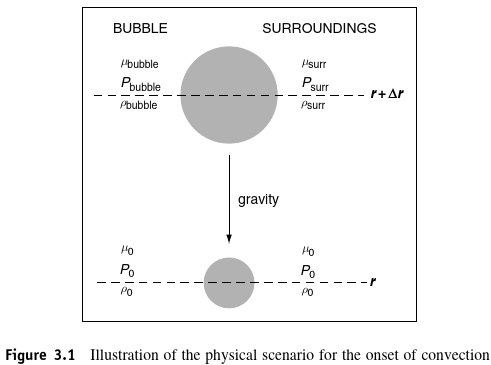
\includegraphics[trim={0cm 0cm 1cm 0cm},clip, keepaspectratio,width=0.99\textwidth]{convectivestability}\label{fig:convectivestability}
\end{figure}
\end{column}\end{columns}
\end{frame}

\begin{frame}{Mixing length: gradiente ambientale e velocit\'a elementi convettivi}
Le stelle con massa $M\leq1.1\msun{}$ hanno una regione radiativa interna mentre la parte esterna \'e convettiva. Convezione esterni $\nabla>\nad$, $v\approx1-10\si{\kilo\meter\per\second}\approx c_s$- $\nabla\to\nad{}$ in interni stellari convettivi: $\TDy{r}{T}=(1-\frac{1}{\Gamma_2})\frac{T}{P}\TDy{r}{P}$, $v\approx\SI{100}{\meter\per\second}\ll c_s$
	\begin{align*}
&F=\frac{L}{4\pi r^2}=F_{rad}+F_{con}=-\frac{4acT^3}{3\kappa\rho}\TDy{r}{T}|_{amb}+\frac{1}{2}\rho vc_p[\TDy{r}{T}|_{Ad}-\TDy{r}{T}|_{amb}]\Lambda\\
&v^2=-\frac{1}{8}g\frac{\Delta\rho}{\rho}\Lambda=\frac{1}{8}g\frac{\Lambda}{H_P}Q(\nabla-\nad),\ Q=1-\TDly{T}{\mu},\ \Lambda=\alpha H_P\\
&F_{con}^{up}=\frac{1}{2}\rho vc_PT\frac{\lambda}{H_P}(\nabla-\nad{})
\end{align*}
\begin{columns}[T]
\begin{column}{0.2\textwidth}
\begin{align*}
&f_r&=-g\Delta\rho(r)=0\tag*{r}\\
&&\propto\Delta r
\end{align*}
\end{column}
\begin{column}{0.8\textwidth}
Work done per unit volume moving bubble of $\Delta r$
\begin{align*}
&W(\Delta r)=-g\int_0^{\Delta r}\Delta\rho(\Delta r')d(\Delta r')=-\frac{1}{2}g\Delta\rho(\Delta r)\Delta r\\
&\exv{W(\Delta r)}_{\Delta r}=\frac{1}{4}W(\Lambda)=\frac{1}{2}\rho v^2
\end{align*}
\end{column}\end{columns}
%Calcolo altezza scala di pressione, flusso convettivo e gradiente ambientale in funzione della velocit\'a media degli elementi
\end{frame}

\begin{wordonframe}{EOS e $\nad{}$}
Considero un'equazione di stato generica $\rho(P,T,\mu)$ e definita tramite:
\begin{align*}
&\frac{d\rho}{\rho}=\alpha\frac{dP}{P}-\delta\frac{dT}{T}+\phi\frac{d\mu}{\mu}\\
&P=\frac{\rho\gasconstant{}T}{\mu}\quad\Rightarrow\quad\alpha=\delta=\phi=1
\end{align*}
Definisco le lunghezze caratteristiche per variazione di densit\'a e pressione:
\begin{equation*}
\densityscale{}=-\frac{dr}{d\ln{\rho}},\ H_P=-\frac{dr}{d\ln{P}}
\end{equation*}
e i gradienti termici per il blob, l'ambiente e il gradiente di composizione chimica ambientale
\begin{equation*}
\nabla=\Dcvar{\TDly{P}{T}}{amb},\ \nabla_e=\Dcvar{\TDly{P}{T}}{e},\ \nmu{}=\Dcvar{\TDly{P}{\mu}}{amb}
\end{equation*}
\end{wordonframe}

\begin{wordonframe}{EOS e EOM}
Riscrivo l'equazione del moto utilizzando l'equazione di stato per scrivere la differenza di densit\'a in termini dei gradienti termici e di composizione chimica; inoltre supponendo il moto dell'elemento in equilibrio di pressione con l'ambiente e assumendo $\nmu{}_{blob}\approx0$ risulta:
\begin{equation*}
\PtwoDy{t}{(\Delta r)}=-g\frac{\delta}{H_P}[\nabla_e-\nabla-\frac{\phi}{\delta}\nmu{}]\Delta r
\end{equation*}
\end{wordonframe}

\begin{wordonframe}{Criterio di \sch/Ledoux}
Infine per ricavare il criterio di stabilit\'a per convezione suppongo  il moto del blob adiabatico:
\begin{equation*}
dq=c_P\,dT-\frac{\delta}{\rho}\,dP
\end{equation*}
da cui risulta:
\begin{equation*}
\nabla_e=\nabla_{ad}=\frac{P\delta}{T\rho c_P}
\end{equation*}
cio\'e una regione solare \'e stabile per convezione se
\begin{equation*}
\nrad{}<\nad+\frac{\phi}{\delta}\nmu{}\label{eq:ledoux}
\end{equation*}
dove ho usato $\nabla_{amb}=\nrad{}$, cio\'e il gradiente che si ha nel caso l'energia sia trasportata dai fotoni.
\end{wordonframe}

\subsection{Teoria della mixing-length.}

\begin{wordonframe}{Convezione in esterni stellari}

In presenza di convezione il flusso di energia verso l'esterno ha una componente radiativa, determinata dal gradiente di temperatura, e una componente dominante convettiva 
\begin{equation*}\label{eq:radconvflux}
F=F_{con}+F_{rad}=\frac{\lsun{}}{4\pi r^2}
\end{equation*}

Una maggiore efficienza del trasporto convettivo di energia si riflette in una minore differenza tra il gradiente di temperature adiabatico ed effettivo.

\begin{figure}[!h]
%   \includegraphics[ width=0.99\textwidth,keepaspectratio]{proportionflux}
%   \subcaption{Profilo radiale (profondit\'a in \si{\kilo\meter}) del flusso convettivo $F_c$ rispetto al flusso totale $F$, della super-adiabaticit\'a $\nabla-\nad{}$ e regioni di ionizzazione idrogeno e $\cel{He}{4}{}{}$. Da \cite{christensen1997effects}.}\label{fluxproportion}

%\includegraphics[keepaspectratio,width=0.9\textwidth]{specificheatnablaa}
%\subcaption{Profilo radiale di $c_P$ e $\nabla_a$: si ha cambiamento di comportamento nelle regioni di ionizzazione parziale di idrogeno ed elio. Da \cite{stix91sun}.}\label{specificheatnablaa}
\end{figure}

Per determinare il gradiente di temperatura effettivo $\nabla$ uso la teoria della mixing-length:
si considera l'eccesso di calore trasportato dai blob di gas nel moto convettivo $c_P\Delta T$ rispetto all'ambiente, il cui cammino libero medio \'e la mixing-length $l_m=\alpha H_P$, che da luogo al flusso di energia
\begin{equation*}
F_{con}=\exv{\rho vc_P\Delta T}\label{eq:convectiveflux}
\end{equation*}
dove $\exv{}$ indica una media opportuna sulla sfera di raggio r. Determino il valor medio della differenza di temperatura prendendo come valore caratteristico dello spostamento del blob $\Delta r\approx\frac{l_m}{2}$:
%, considerando moti in entrambi i versi,
\begin{equation*}
\frac{\Delta T}{T}\approx\frac{1}{T}\PDy{r}{(\Delta T)}\frac{l_m}{2}=(\nabla-\nabla_e)\frac{l_m}{2}\frac{1}{H_P}\label{eq:blobambdiff}
\end{equation*}

Assumo il lavoro medio fatto dalla forza di galleggiamento per unit\'a di massa $-g\frac{\Delta\rho}{\rho}$ uguale al valore medio della forza, cio\'e la met\'a di quello alla superficie sferica data, moltiplicato lo spostamento medio $\frac{l_m}{2}$ quindi, assumendo in oltre che in media met\'a del lavoro fatto dalla forza di galleggiamento sia trasformato in energia cinetica del blob si ottiene
\begin{equation*}
v^2=g\delta(\nabla-\nabla_e)\frac{l_m^2}{8H_P}\label{eq:blobvelocity}
\end{equation*}

Infine determino gli scambi radiative del blob: il modulo del flusso radiativo \'e proporzionale al gradiente termico in direzione normale alla superficie del blob
\begin{equation*}
f=\frac{4acT^3}{3\kappa\rho}|\PDy{n}{T}|
\end{equation*}
quindi l'energia scambiata dall'intera superficie S del blob \'e $\lambda=Sf$ che determina, per la prima legge della termodinamica, una variazione di temperatura per unit\'a di tempo:
\begin{equation*}
\PDy{t}{T_e}=-\frac{\lambda}{\rho Vc_P}
\end{equation*}
indicato con $V$ il volume del blob.

La variazione della temperatura del blob per unit\'a distanza percorsa \'e quindi
\begin{equation*}
\Dcvar{\TDy{r}{T}}{e}=\Dcvar{\TDy{r}{T}}{ad}-\frac{\lambda}{\rho Vc_Pv}\label{eq:Tchangelength}
\end{equation*}
e approssimando il gradiente normale alla superficie con $\exv{\Delta T}$ ed usando le definizioni \eqref{eq:nablavitense} si ottiene:
\begin{equation*}
\frac{\nabla_e-\nad{}}{\nabla-\nabla_e}=\frac{6acT^3}{\kappa\rho^2c_Pl_mv}
\end{equation*}
Il gradiente termico ambientale $\nabla$ e del blob $\nabla_e$ sono determinati da \eqref{eq:radconvflux} e \eqref{eq:Tchangelength} inserendo le espressioni per il flusso radiativo \eqref{eq:radiativeflux} e il flusso convettivo \eqref{eq:convectiveflux}.

In figura (\subref{fluxproportion}) si mostrano l'andamento di $\nabla-\nad{}$, il profilo termico e la frazione di flusso totale trasportato dalla convezione; in figure (\subref{specificheatnablaa}) si mostrano il profilo del calore specifico per unit\'a di massa e del gradiente adiabatico.

Le 5 equazioni del flusso convettivo

Le 5 equazioni determinano completamente le variabili $F_{rad}, F_{con}, v, \nabla_e, \nabla$ in funzione di $P,T,l(r),m(r),c_P,\nad{},\nrad{},g$.

Come determino il gradiente effettivo ??

Determino $\nabla-\nabla_e$
cubic equation for $(\nabla-\nabla_e)$

\end{wordonframe}

\subsection{Approssimazione politropa}\linkdest{poly}

\begin{frame}{Trasformazioni politropiche}
\begin{block}{Gener. T. adiabatica}
	Il rapporto $\gamma=\frac{c_P}{c_V}$ costante per gas perfetto di sole particelle totalmente ionizzato.
	T. adiabatica:
	\[TV\expy{\gamma-1}=\const,\ PV\expy{\gamma}=\const,\ P\expy{1-\gamma}T\expy{\gamma}=\const\]
$0=dE-\frac{P}{\rho^2}d\rho$
Caso pi\'u generale delle trasformazioni adiabatiche: \keyword{trasformazione politropa} trasformazione quasi-statica in maniera che $c=\TDy{Q}{T}$ (calore specifico) vari in maniera assegnata. (adiabatica: $c=0$, isoterma: $c=\infty$, isometrica: $c=c_V$, ...)
\end{block}
\begin{block}{Relazione politropa - EOS}
\begin{columns}[T]
	\begin{column}{0.4\textwidth}
\begin{align*}
&\TDy{r}{P}=-\TDy{r}{\phi}\rho\\
&\frac{1}{r^2}\TDof{r}(r^2\TDy{r}{\phi})=4\pi G\rho\\
&\TDy{r}{\phi}=-\gamma K\rho\expy{\gamma-2}\TDy{r}{\rho}
\end{align*}
\end{column}
\begin{column}{0.6\textwidth}
\begin{align*}
&P=K\rho\expy{\gamma}=K\rho\expy{1+1/n}\\
&\gamma=5/3, n=3/2\tag{NR deg}\\
&\gamma=4/3, n=3\tag{R deg}\\
&\gamma=1, n=\infty\tag{isot.}\\
&\nad\approx\frac{2}{5}\tag{conv}\\
&P\propto\rho\expy{5/3}
\end{align*}
For convective exponent K varies from star to star
\end{column}\end{columns}
\end{block}
\end{frame}

\begin{frame}{Equazione Lane-Emden}
\begin{columns}[T]
	\begin{column}{0.5\textwidth}
\begin{align*}
&\rho=(\frac{-\phi}{(n+1)K})^n\tag{HE}\\
&\TtwoDy{r}{\phi}+\frac{2}{r}\TDy{r}{\phi}=4\pi G(\frac{-\phi}{(n+1)K})^n\tag{Poiss}\\
&\TtwoDy{z}{w}+\frac{2}{z}\TDy{z}{w}+w^n=0\\
&\frac{1}{z^2}\TDof{z}(z^2\TDy{z}{w})+w^n=0\tag{Lane-Emden}
\end{align*}
	\end{column}
	\begin{column}{0.5\textwidth}
		\begin{align*}
	&z=Ar\tag{new vars}\\
	&A^2=\frac{4\pi G}{(n+1)^nK^n}(-\phi_c)\expy{n-1}\\
	&=\frac{4\pi G}{(n+1)K}\rho_c\expy{\frac{n-1}{n}}\\
	&w=\frac{\phi}{\phi_c}=(\frac{\rho}{\rho_c})\expy{1/n}
		\end{align*}
\end{column}\end{columns}
\end{frame}

\begin{frame}{Strutture isoterme e modello solare}

\end{frame}

\subsection{Equazione di stato}\linkdest{eos}

\begin{wordonframe}{Schema fisico/chimico: ingredienti EOS realistiche}
\begin{itemize}
\item schema chimico: il primo considera atomi e molecole, la cui popolazione per stati eccitati e diversi gradi di ionizzazione \'e ottenuto minimizzando l'energia libera da cui sono ricavate le altre grandezze termodinamiche; utilizzando questo approccio \'e stata ricavata l'equazione di stato MHD (\cite{hummer1988equation})
\item schema fisico: nuclei ed elettroni come costituenti fondamentali interagenti tramite potenziale Coulombiano e trova le soluzione dell'equazione di Schr\"oedinger per un problema a molti corpi, questo approccio, usato per ricavare l'equazione di stato OPAL (\cite{rogers1986occupation})
\end{itemize}


Come illustrato in figura, per entrambe $\Gamma_1\approx\midfrac{5}{3}$ nell'interno solare e maggiori deviazioni si hanno nelle regioni di ionizzazione parziale degli elementi in particolare di idrogeno ed elio.
\end{wordonframe}

\begin{wordonframe}{Relazione tra $P(\rho, T)$: approx zero gas perfetto di atomi completamente ionizzati}
\begin{columns}[T]
\begin{column}{0.55\textwidth}
EOS gas perfetto di ioni ed elettroni 
\begin{equation*}
P_G=P_I+P_e=\frac{\rho}{\mu}\gasconstant{}T
\end{equation*}
Energia interna per unit\'a di massa: somma delle energie traslazionali delle particelle pesate secondo la distribuzione di equilibrio di Maxwell-Boltzmann per grammo di materia
\begin{align*}
&u=\frac{1}{\rho}\sum_i\int f^{(0)}(\vec{p}_i)\frac{p^2_i}{2m_i}\,d^3p_i\\
&=\frac{3}{2}\frac{P}{\rho}=\frac{3}{2}\frac{\gasconstant T}{\mu}
\end{align*}
\end{column}
\begin{column}{0.45\textwidth}
Peso molecolare medio: massa media in amu per particella libera
\begin{align*}
&\mu=\frac{1}{\bar{n}_HX+\bar{n}_{He}Y+\bar{n}_{Z}Z}\\
&\mu_0=\frac{1}{X+\midfrac{Y}{4}+\midfrac{Z}{\bar{A}}},\ \mu_e\approx\frac{2}{1+X}
\end{align*}
con $\bar{n}_i=\frac{1+f_i}{A_i}$ numero medio di particelle libere per unit\'a di massa atomica dovute alla specie i di peso atomico $A_i$ e $f_i$ numero medio di elettroni liberati da ione della specie i; peso atomico medio per ione $\mu_0$ ed elettrone libero (ionizzato) $\mu_e$.
\end{column}
\end{columns}
$f^{(0)}(\vec{p}_i)$: numero di particelle della specie i per unit\'a di volume con impulso in $[\vec{p}_i,\vec{p}_i+d\vec{p}_i]$
\end{wordonframe}

\begin{wordonframe}{Deviazioni dalla legge dei gas perfetti: radiazione e degenerazione elettronica}
\begin{itemize}
	\item Radiazione. Il contributo alla pressione ed energia interna per unit\'a di volume dei fotoni $P_R=\frac{a}{3}T^4$, $u_R=aT^4$, e $P-P_R=\beta P$.
	\item Degenerazione elettronica - Principio di Pauli: non pi\'u di 2 elettroni in volume di spazio delle fasi $h^3$. $n_e$ la densit\'a numerica di \Pelectron, $\psi(P,T)$ il parametro di degenerazione, tale che per $\psi\to-\infty$ si abbia la distribuzione di Boltzmann e per $\psi\to+\infty$ completa degenerazione
	\begin{align*}
	&n_e=\rho N_A\frac{1+X}{2}=\intzi{}\frac{8\pi p^2\,dp}{h^3(\exp{\frac{u_k}{KT}-\psi}+1)}=\frac{8\pi}{h^3}(2m_ekT)\expy{3/2}a(\psi)\\
	&P_e=\beta P-\rho\gasconstant{}(X+\frac{Y}{4}+\frac{Z}{\exv{A_Z}})=\frac{8\pi}{3h^3}\intzi{}p^3v(p)\frac{dp}{1+\exp{\epsilon/kT-\psi}}\\
	&U_e=\frac{8\pi}{h^3}\int_0^{\infty}\frac{p^2\epsilon(p)\,dp}{\exp{(-\psi+\midfrac{\epsilon}{KT})}+1}
	\end{align*}
\end{itemize}
\end{wordonframe}

\begin{frame}{degenerazione completa: casi limite NR e R}
\begin{align*}
&P_e=\int_{2\pi}\frac{d\Omega}{4\pi}\intzi{}dpf(p)v(p)p^2\cos{\theta}=\frac{8\pi}{3h^3}\int_0^{P_F}p^3v(p)\,dp\\
&=\frac{8\pi c}{3h^3}\int_0^{P_F}\frac{p/(m_ec)}{\sqrt{1+p^2/(m_ec)^2}}=\frac{\pi m_e^4c^5}{3h^2}f(x)\\
&U_e=\int_0^{P_F}f(p)E(p)\,dp=\frac{8\pi}{h^3}\int_0^{P_F}E(p)p^2\,dp=\frac{\pi m_e^4c^5}{3h^3}g(x)\
\end{align*}
\begin{align*}
&n_e=\frac{\rho}{\mu_em_H}=\frac{8\pi m_ec^3}{3h^3}x^3\\
&x=\frac{P_F}{m_ec}\ll1:\quad&x\gg1:\\
&P_e=\frac{8\pi m_e^4c^5}{15h^3}x^5=\frac{2}{3}U_e&P_e=\frac{2\pi m_e^4c^5}{3h^3}x^4=\frac{1}{3}U_e\\
&=\num{1.0036e13}(\frac{\rho}{\mu_e})\expy{5/3}&=\num{1.2435e15}(\frac{\rho}{\mu_e})\expy{4/3}
\end{align*}
\end{frame}

\begin{wordonframe}{Elettrostatic screening of ions: weak screening}
La principale correzione che tiene conto dell'interazioni tra particelle \'e dovuta alle interazioni coulombiane: influence EOS and nuclear rection rates.

Screening of ion i with charge $Z_ie$ ar $\vec{r_i}$ in NR dilute plasma, motion of screened ions is slow compared to screening particles: continuum static equilibrium charge distribution (\Pelectron, light ions of mean charge $Z_p$)
\begin{equation*}
\nabla^2\phi=4\pi n_ee[\exp{(\frac{e\phi}{kT})}-\exp{-\frac{Z_pe\phi}{kT}}]-4\pi\sum_iZ_ie\delta(\vec{r}-\vec{r_i})
\end{equation*}
Regime di schermaggio debole, $e\phi\ll KT$: $\phi=\sum_i\phi_i$ potenziale attorno a ione pesante isolato:
\begin{align*}
%&\nabla^2\phi=-4\pi e\sum_Z Zn_Z-4\pi e\sum_i Z_i\delta(\vec{r}-\vec{r}_i)\\
&\phi_i=\frac{Z_ie}{r_i}\exp{-\frac{r_i}{r_D}}
&\frac{1}{r_D^2}=\frac{4\pi e^2}{kT}\sum Z^2\overline{n}_Z=\frac{4\pi e^2}{kT}N_A\zeta,\ \zeta=\sum_{i}(Z_i^2+Z_i)\frac{\rho X_i}{A_i}
\end{align*}
\end{wordonframe}

\begin{wordonframe}{Elettrostatic screening of ions: energy pressure correction}
Energy required to assemble uniform shere with charge $Ze$: $U_{ee}=\int_0^{R_Z}\frac{q_r}{r}\,dq=\frac{3}{5}\frac{(Ze)^2}{R_Z}$.
Energy required to assemble uniform cloud of charge $Ze$ around Z-nucleus: $U_{eZ}=-Ze\int_0^{R_Z}\frac{dq}{r}=-\frac{3}{2}\frac{(Ze)^2}{R_Z}$
Le correzioni dovute alle interazioni coulombiane sono dovute a numero sfere ioniche per unit\'a di volume $n_Z=\frac{\rho X_Z}{A_Z}N_0$ with average potential energy per electron $\exv{-e\phi}_Z=-\frac{9}{10}\frac{(Ze)^2}{R_Z}$ that contain Z \Pelectron.
\begin{align*}
&\rho u_c=(\frac{U}{V})_e=\frac{1}{2}\phi(\vec{r})\rho_c(\vec{r})\to \frac{1}{2}\sum_ZeZ\overline{n}_Z\phi_Z=-e^3\sqrt{\frac{\pi\rho}{kT}}(N_A\zeta)\expy{\frac{3}{2}},\ P_c=\frac{1}{3}\rho u_c\\
&E_0=\frac{(U/V)_e}{n_e}=\mu_e\sum_Z\exv{-e\phi}_Z\frac{ZX_Z}{A_Z}\approx-1.3(\mu_e^2\rho)\expy{1/3}[X+0.79Y+\sum_{Z>2}\frac{Z\expy{5/3}X_Z}{A_Z}]
\end{align*}
\end{wordonframe}

\begin{frame}{Equazione di Saha e continuum depression. Ioniozzazione da pressione}
L'equazione di Saha descrive la frazione relativa di ionizzazione
\begin{align*}
&\frac{n_{r+1}}{n_r}n_e=\frac{g_{r+1}}{g_r}f_r(T)\\
&f_r(T)=2\frac{(2\pi m_ekT)\expy{3/2}}{h^3}\exp{-\chi_r/(kT)}
\end{align*}
Saha limitation:
\begin{itemize}
\item LTE: is the case when collision dominate over radiative processes
\item Decreases ionization energy with increasing density: what is called pressure ionizzation is produced by coulomb interaction of bound electron with other electron in the plasma $\chi'_Z=\chi_Z-\frac{Ze^2}{R_D}$
\end{itemize}
\end{frame}

\begin{frame}{Crystallization and Neutronization}
\begin{block}{Crystallization}
Per $\rho$ alta e $T$ bassa (WD interior: $\Gamma_c=\frac{(Ze)^2}{r_{ion}kT}\approx180$) gli ioni formano reticolo quando energia termica uguale interazione coulombiana $\frac{3}{2}kT\approx E_c$ - melting $T_m\approx\frac{Z^2e^2}{\Gamma_ck}(\frac{4\pi\rho}{3\mu_0m_H})\expy{1/3}=\num{2.3e3}Z^2\mu_0\expy{-1/3}\rho\expy{1/3}$
\end{block}
\begin{block}{Neutronization}
If \Pelectron have $E_e>E^*=c^2(m_n-m_p)\approx\SI{1.3}{\mega\ev}$ they combine with protons and form neutrons: if we put $E=E_{kin}+m_ec^2=E_F+m_ec^2=c^2(m_n-m_p)\approx\SI{1.3}{\mega\ev}$ if $E_{kin}<E_F$ l'elettrone non trova stati liberi e il neutrone non decade ($x=\frac{p_F}{m_ec}\approx2.2$).
For $\rho>\SI{4e11}{\gram\per\cubic\cm}$ we have inverse $beta$-decay:nuclei capture electron and become neutron rich - neutron drip
\end{block}
\end{frame}

\section{Energy production}\linkdest{luminositysourcessinks}

\subsection{Work against gravity}\linkdest{epsilong}

\begin{frame}{Work done in expansion/contraction: }

\end{frame}

\subsection{Fusione nucleare}\linkdest{epsilonn}

\begin{frame}{Sezione d'urto fusion nucleare}
$E$ l'energia cinetica nel centro di massa dei nuclei: $\sigma(E)=\pi\lambdabar^2*P_0(E)*S(E)$
prodotto della sezione d'urto geometrica (nel riferimento del CM: $\sigma\approx\sum_{l=0}^{\frac{R}{\lambdabar}}(2l+1)\pi\lambdabar^2=\pi(R+\lambdabar)^2$
per energie tipiche degli interni stellari approx onda S), della probabilit\'a di attraversamento della barriera coulombiana e del fattore astrofisico. La lunghezza d'onda di de Broglie relativa delle particelle descrive l'indeterminazione sulla posizione nell'urto di due particelle con momento relativo p $\lambdabar=\frac{\hbar}{p}=\frac{\hbar}{\sqrt{2mE}}$.

L'energia potenziale dovuta all'interazione di due nuclei $Z_1$ e $Z_2$ a distanza r contiene un contributo delle altre cariche presenti nel plasma $U=\frac{Z_1Z_2e^2}{r}+U_s(r_{12})$
l'energia potenziale non schermata e contributo della nuvola elettronica: $U_s$ aumenta la probabilit\'a di attraversamento della barriera coulombiana. Fattore moltiplicativo: $f=\exp{-\midfrac{U_0}{KT}}$ dove $U_0=U_s(0)$ poich\'e $r\ll r_D$ e considerando solo la correzione al fattore di penetrazione ($E_G\gg U_0$).

Per determinare $U_0$ considero l'energia potenziale di $Z_1$ e $Z_2$ a distanza $r$
\begin{equation*}
U=Z_2e\int_{\infty}^r\PDy{r_1}{\phi_1}\,dr_1=\frac{Z_1Z_2e^2\exp{-\midfrac{r}{r_D}}}{r},\ U_s=U-\frac{Z_1Z_2e^2}{r}\approx\frac{Z_1Z_2e^2}{r_D}
\end{equation*}
\end{frame}

\begin{frame}{Energia prodotta in reazioni di fusione???}
$S(E)$ descrive l'interazione a livello nucleare: debolmente dipendente dall'energia in assenza di risonanze.
La probabilit\'a di attraversamento della barriera coulombiana: $P_0(E)=\exp{-2\pi\eta},\ \eta=\sqrt{\frac{m}{2}}\frac{Z_1Z_2e^2}{\hbar E\expy{\frac{1}{2}}}$
Per i nuclei di carica $Z_1$, $Z_2$ e m massa ridotta: $\sigma(E)=\frac{S(E)}{E}\exp{-2\pi\eta}$
Il rate per coppia di particelle
\begin{equation*}
\exv{\sigma v}=\num{1.3005e-15}[\frac{Z_1Z_2}{AT_6^2}]\expy{\frac{1}{3}}fS_{eff}\exp{-\tau}\si{\cubic\cm\per\second},\ \tau=\frac{3E_G}{kT}\approx\num{42.487}(Z_1^2Z_2^2AT_6\expy{-1})\expy{\frac{1}{3}}
\end{equation*}
$S_{eff}$ \'e il risultato dell'espansione dell'integrando per $\invers{\tau}\ll1$ ed estrapolato a $E_G$ a partire dal valore $S(0)$ determinato dalla fisica nucleare.
La funzione $\epsilon(\rho,T,X_i)$ \'e determinata dalla somma di tutti i contributi
\begin{equation*}
\epsilon_{ij}=Q_{ij}\frac{n_in_j}{\rho(1+\delta_{ij})}\lambda_{ij}=\frac{1}{1+\delta_{ij}}Q_{ij}\frac{\rho N_A^2X_jX_k}{{A_iA_j}}\exv{\sigma v}_{ij}\label{eq:energyrate}
\end{equation*}
dove $Q_{ij}$ \'e l'energia liberata per reazione tra nucleo di specie i e j e $\exv{\sigma v}_{ij}$ \'e il rate di reazione per coppia di particelle, mediata su MB- distro
$f(E)dE\propto\frac{E\expy{\frac{1}{2}}}{(kT)\expy{\frac{3}{2}}}\exp{-\frac{E}{kT}}\,dE$:
$S(E)\exp{-\frac{E}{kT}-\frac{b}{\sqrt{E}}}$
ha forma approssimativamente gaussiana il cui massimo $E_G$, energia pi\'u probabile di reazione, e FWHM sono: $E_G=\SI{5.665}{\kilo\ev} A\expy{\frac{1}{3}}T_7\expy{\frac{2}{3}}$ $\Delta E=4.249\si{\kilo\ev}W\expy{\frac{1}{6}}T_7\expy{\frac{5}{6}}$
posto $W=Z_i^2Z_j^2A=Z_i^2Z_j^2\frac{A_iA_j}{A_i+A_j}$.
%\begin{equation*}
%\exv{\sigma v}\propto b\expy{1/3}T\expy{-2/3}\exp{-\frac{b\expy{2/3}}{t\expy{1/3}}}
%\end{equation*}
\end{frame}

\subsection{Catena PP}\linkdest{epsilonpp}

\begin{frame}{PP1: twice $\Pproton(\Pproton,\Pnue\APelectron)d(p,\gamma)^3He$ and $^3He(^3He,21^H)^4He$}
\begin{columns}[T]
	\begin{column}{0.55\textwidth}
\begin{itemize}
	\item $\tau_p(d)\ll[\tau_{^3He}(d)]_e\ll[\tau_d(d)]_e$: $\frac{\dot{D}}{H}=\frac{H}{2}\exv{\sigma v}_{pp}-H(\frac{D}{H})\exv{\sigma v}_{dp}$ - \keyword{D evolution} $(\frac{D}{H})=\frac{\exv{\sigma v}_{pp}}{2\exv{\sigma v}_{dp}}$, evolution: $(\frac{D}{H})_t=(\frac{D}{H})_e-[(\frac{D}{H})_e-(\frac{D}{H})_0]\exp{-\frac{t}{\tau_p(d)}}$
	\item \keyword{$^3He$ evolution} - $\frac{\dot{^3He}}{H}=\frac{H}{2}\exv{\sigma v}_{pp}-H(\frac{^3He}{H})^2\exv{\sigma v}_{^3He^3He}$ - 
\scalebox{0.8}{	\[\frac{^3He}{H}|_t=0+\sqrt{\frac{\exv{\sigma v}_{pp}}{\exv{\sigma v}_{^3He^3He}}}\tanh(t\sqrt{\frac{H}{2}\exv{\sigma v}_{PP}H\exv{\sigma v}_{^3He^3He}})\]}
\item Produzione energia - $\epsilon_{PPI}^e(T_0=\SI{15}{\mega\ev})(\frac{T}{T_0})\expy{3.9}$
\begin{align*}
&\epsilon_{PPI}=\frac{(6.936-0.265)\si{\mega\ev}H^2\exv{\sigma v}_{pp}}{2\rho}\\
&+\frac{\SI{12.861}{\mega\ev}H^2\exv{\sigma v}_{^3He^3He}}{2\rho}(\frac{^3He}{H})^2\\
&\epsilon_{PPI}^e(T)=6.551N_A\exv{\sigma v}_{PP}(\frac{X_H}{m_H})^2\rho N_A\frac{\si{\mega\ev}}{\si{\second\gram}}
\end{align*}
\end{itemize}
	\end{column}
	\begin{column}{0.45\textwidth}
	\begin{figure}[!ht]
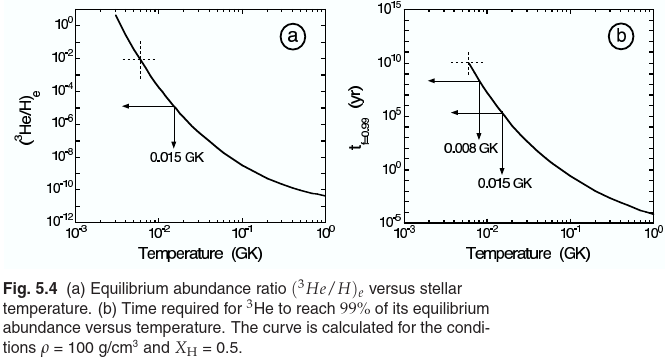
\includegraphics[trim={0cm 0cm 1cm 0cm},clip, keepaspectratio,height=0.28\textheight]{He3eq}
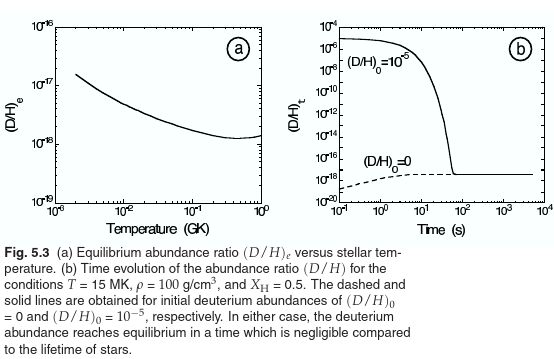
\includegraphics[trim={0cm 0cm 1cm 0cm},clip, keepaspectratio,height=0.28\textheight]{PP1DHet}
\includegraphics[trim={0cm 0cm 1cm 0cm},clip, keepaspectratio,height=0.28\textheight]{pplifetime}
	\end{figure}
	\end{column}
\end{columns}
\end{frame}

\begin{frame}{Network reazioni PP completo}

\begin{columns}[T]
\begin{column}{0.55\textwidth}
Rapid $^8B/^8Be$ decays: $^7Be(p,\gamma)^8B(\APelectron,\nu)^8Be(\alpha)\alpha$ as $^7Be+p\to2\alpha+\gamma$, $\TDof{t}(^7Li+^7Be)\approx0$
\begin{align*}
&Q_{PPI}=27.73-2\exv{E}_{\nu}^{pp}=\SI{26.19}{\mega\ev}\\
&Q_{PPII}=26.73-\exv{E}_{\nu}^{^7Be}-\exv{E}_{\nu}^{pp}=\SI{25.65}{\mega\ev}\\
&Q_{PPIII}=26.73-\exv{E}_{\nu}^{^8B}-\exv{E}_{\nu}^{pp}=\SI{19.75}{\mega\ev}\\
&\epsilon_{PP}=\frac{Q_{4H\to^4He}}{\rho}\dot{^4He}[0.98F_{PPI}+0.96F_{PPII}\\
&+0.74F_{PPIII}],\ f_{PPI}=\frac{r_{^3He^3He}}{r_{^3He^3He}+r_{\alpha^3He}}\\
&F_{PPII}=(1-F_ {PPI})\frac{r_{e^7Be}}{r_{e^7Be}+r_{p^7Be}}
\end{align*}
\end{column}
\begin{column}{0.45\textwidth}
\begin{figure}[!ht]
	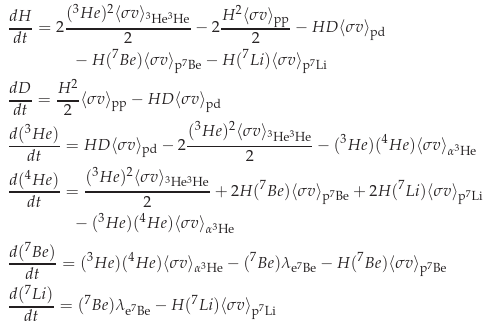
\includegraphics[trim={0cm 0cm 1cm 0cm},clip, keepaspectratio,width=0.72\textwidth]{ppchainsequi}
	\includegraphics[trim={0cm 0cm 1cm 0cm},clip, keepaspectratio,width=0.72\textwidth]{ppfraction}
\end{figure}
\end{column}
\end{columns}
\begin{align*}
&\dot{(^3He)}=\frac{H^2}{2}\exv{\sigma v}_{pp}-2(^3He)^2\frac{\exv{\sigma v}_{^3He^3He}}{2}-(^3He)(^4He)\exv{\sigma v}_{\alpha^3He}\\
&(^3He)_e=\frac{-(^4He)\exv{\sigma v}_{\alpha^3He}+\sqrt{(^4He)^2\exv{\sigma v}_{\alpha^3He}^2+2H^2\exv{\sigma v}_{\alpha^3He}\exv_{\sigma v}_{^3He^3He}}}{2\exv{\sigma v}_{^3He^3He}}
\end{align*}
\end{frame}


\subsection{Ciclo CN-NO:}\linkdest{epsilonCNO}

\begin{frame}{Biciclo CNO}
dipendenza da T
flusso neutrini
Modalit\'a combustione H in He: sequenza principale inferiore/superiore
\end{frame}

\begin{frame}{CNOF Network reactions: $4^1H\to^4He+2\APelectron+2\Pnue$}
\begin{columns}[T]
\begin{column}{0.5\textwidth}
\begin{itemize}
\item CNOF elements acts as catalyst: relative initial CNOF abundance are important - produced in previous gen stars at He-burning stages ($^{12}C$, $^{16}O$, less $^{14}N$: solar $^{12}C:^{14}N:^{16}O=10:3:24$)
\item 4 cycle: active cycle influences heavy element abundance - $(p,\gamma)$ compete with $(p,\alpha)$ on $^{15}N$, $^{17}O$, $^{18}$, $^{19}F$: $(p,\alpha)$ faster over entire T-range except $^{17}O$/$^{18}O$ at $T<\SI{20}{\mega\kelvin}$
\item At hydro-burning ($T<\SI{55}{\mega\kelvin}$) much faster than p-induced reactions, at $T>\SI{100}{\mega\kelvin}$ also other reactions are important (HCNO)
\end{itemize}
\end{column}
\begin{column}{0.5\textwidth}
	\begin{figure}[!ht]
	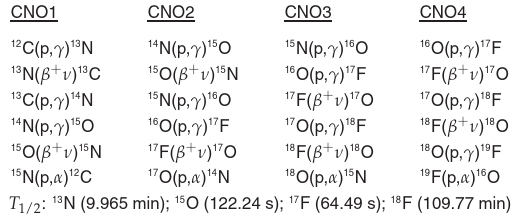
\includegraphics[trim={0cm 0cm 1cm 0cm},clip, keepaspectratio,height=0.28\textheight]{CNO}
	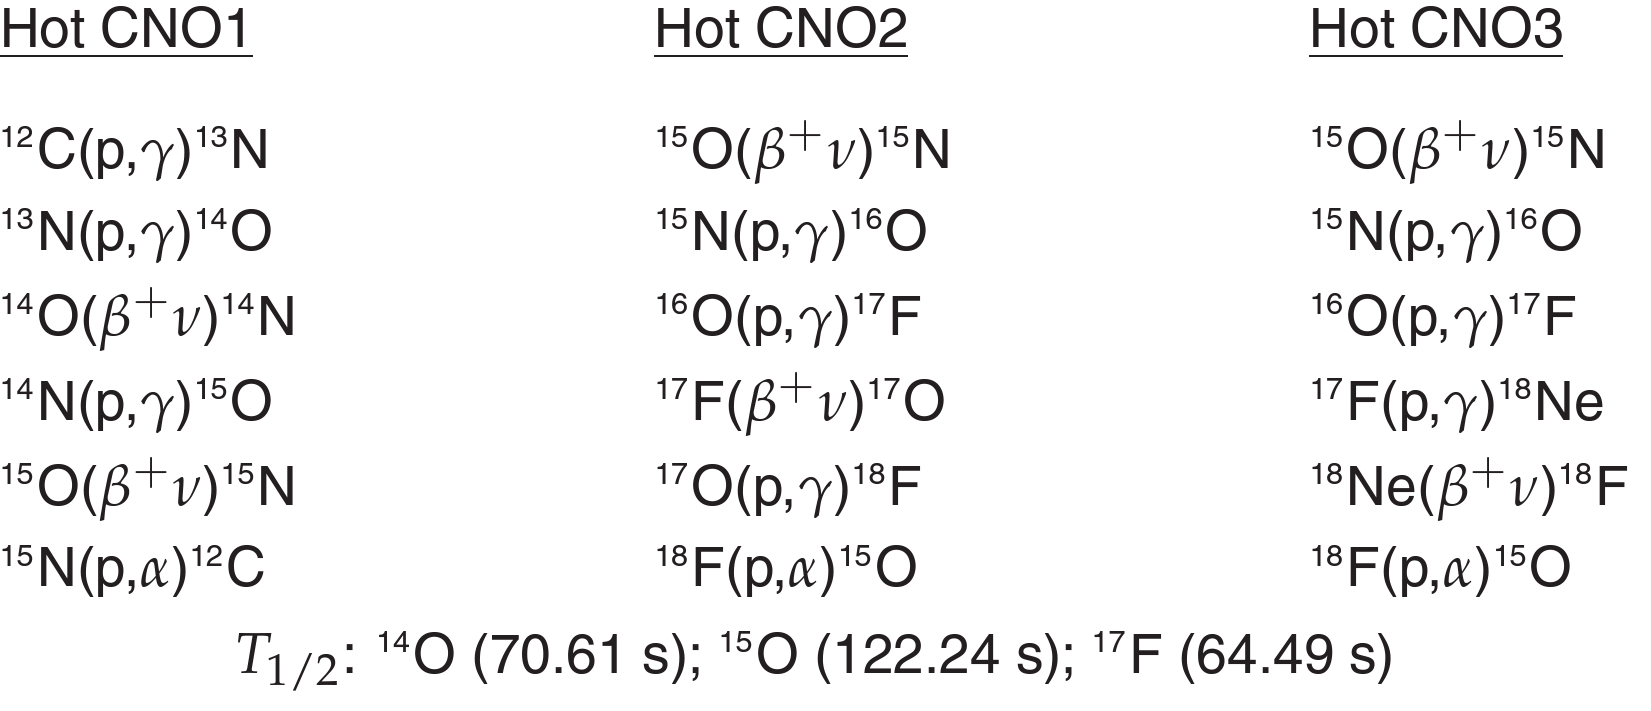
\includegraphics[trim={0cm 0cm 1cm 0cm},clip, keepaspectratio,height=0.28\textheight]{HCNO}
\end{figure}
\end{column}
\end{columns}
\end{frame}

\begin{frame}{CNO1: equilibrium properties}
\begin{columns}[T]
	\begin{column}{0.5\textwidth}
		\begin{itemize}
			\item Elements involving beta-decay reaches equilibrium in few minutes: $\dot{^{13}N}=0$ - $(^{13}N)_t=\frac{\tau_{\beta}(^{13}N)}{\tau_p{^{12}C}}^{12}C[1-\exp{-\frac{t}{\tau_{\beta}(^{13}N)}}]$ - $(\frac{^{13}N}{^{12}C})_e=\frac{\tau_{\beta}(^{13}N)}{\tau_p(^{12}C)}$
			\item At equilibrium ratio of abundance of $^{12}C$, $^{13}C$, $^{14}N$, $^{15}N$ are given by inverse ratio of reaction time (ie $(\frac{^{14}N}{^{12}C})_e=\frac{\exv{\sigma v}_{^{12}C(p,\gamma)}}{\exv{\sigma v}_{^{14}N(p,\gamma)}}=\frac{\tau_p(^{14}N)}{\tau_p(^{12}C)}$), fractional abundance $\frac{(^{12}C)_e}{\sum CNO1}=\frac{\tau_p(^{12}C)}{\tau_p(^{12}C)+\tau_p(^{13}C)+\tau_p(^{14}N)+\tau_p(^{15}N)}$
		\end{itemize}
	\end{column}
	\begin{column}{0.5\textwidth}
		\begin{figure}[!ht]
			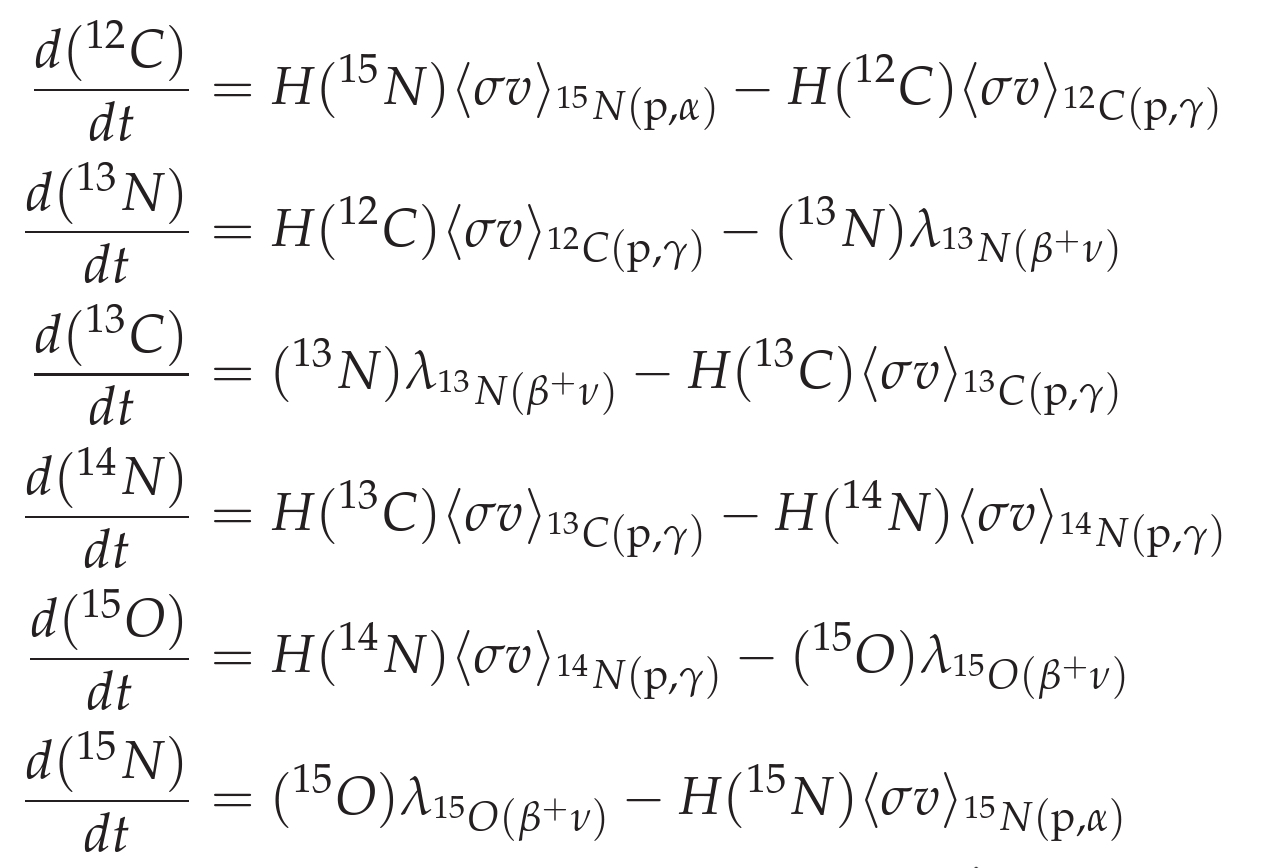
\includegraphics[trim={0cm 0cm 1cm 0cm},clip, keepaspectratio,height=0.28\textheight]{CNO1ab}
			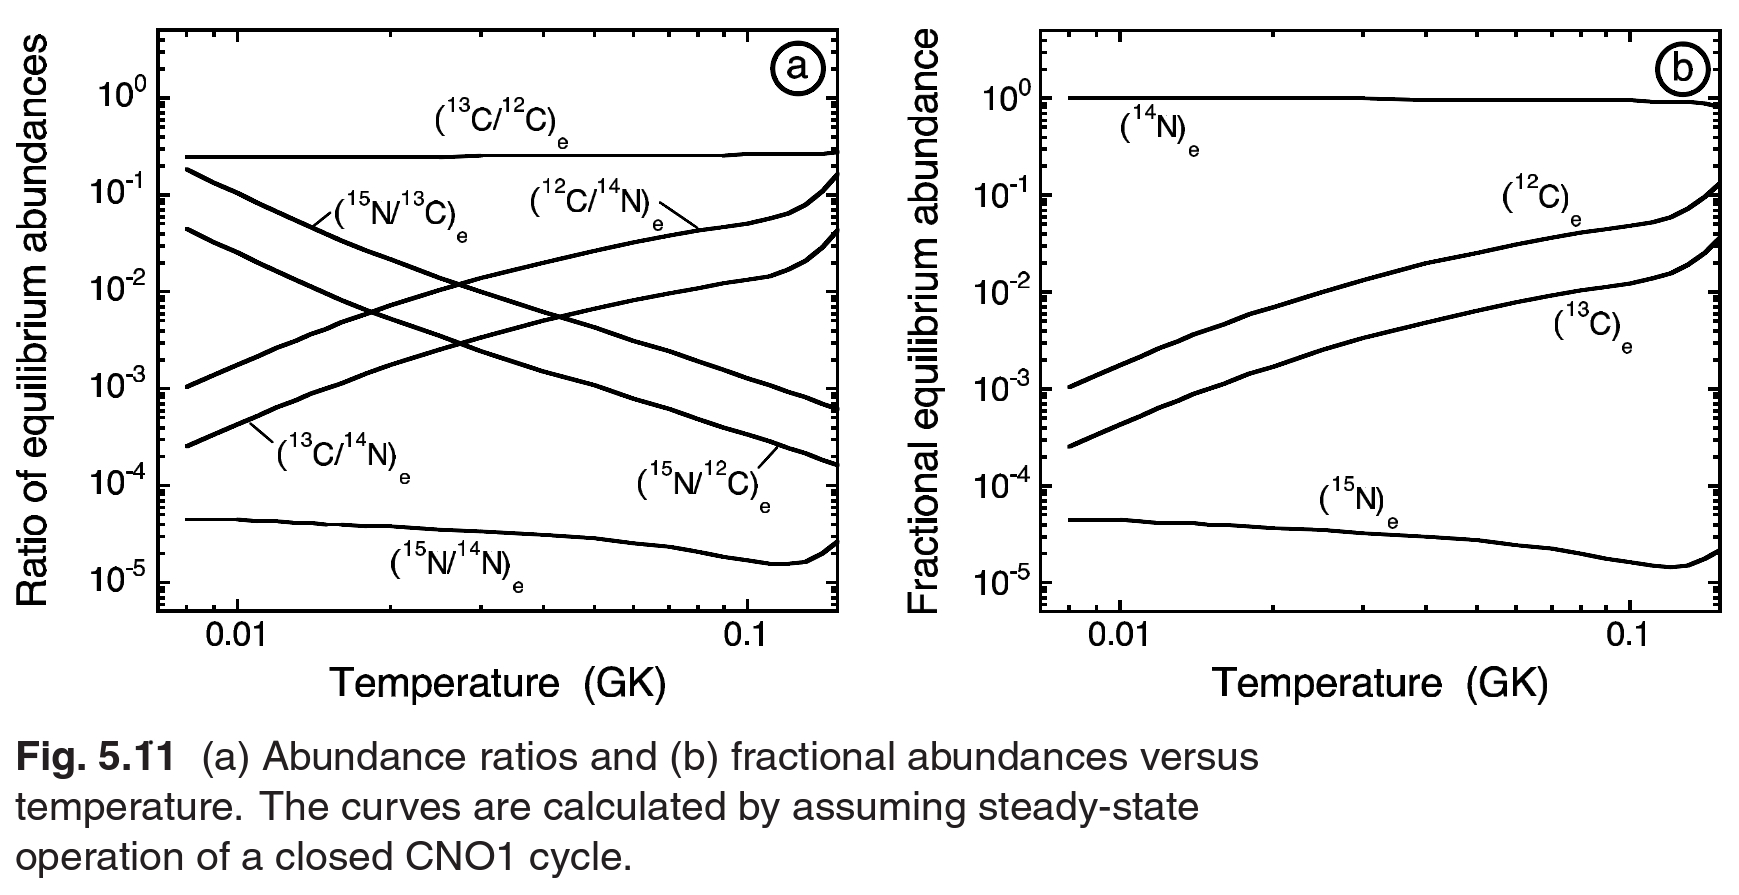
\includegraphics[trim={0cm 0cm 1cm 0cm},clip, keepaspectratio,height=0.28\textheight]{CNOXivsT}
		\end{figure}
	\end{column}
\end{columns}
\end{frame}

\begin{frame}{CNO1: energy production rate}

\begin{align*}
&\epsilon_{CNO1}=\sum_{i\to j}\epsilon_{i\to j}=\frac{1}{\rho}(Q_{i\to j}-\exv{E}_{\nu}^{i\to j})r_{i\to j}\\
&\rho\epsilon^e_{CNO1}=\SI{3.458}{\mega\ev}\frac{(^{12}C)_e}{\tau_p(^{12}C)}+\SI{7.551}{\mega\ev}\frac{(^{13}C)_e}{\tau_p(^{13}C)}+\SI{9.055}{\mega\ev}\frac{(^{14}N)_e}{\tau_p(^{14}N)}\\
&+\SI{4.966}{\mega\ev}\frac{(^{15}N)_e}{\tau_p(^{15}N)}\\
&\epsilon^e_{CNO1}\approx\SI{25.030}{\mega\ev}N_A\exv{\sigma v}_{^{14}N(p,\gamma)}(\sum_{CNO1}\frac{X_i}{M_i})\frac{X_H}{M_H}\rho N_A\si{\mega\ev\per\second\per\gram}\\
&\epsilon^e_{CNO1}=\epsilon^e_{CNO1}(T_0)(\frac{T}{T_0})\expy{16.7},\ T_0\approx\SI{25}{\mega\kelvin}\\
%%Q
&Q_{^{12}C(p,\gamma)^{13}N(\beta^+\nu)}-\exv{E}_{\nu}^{^{13}N(\beta^+\nu)}=(1.944+2.22-0.706)\si{\mega\ev}\\
&Q_{^{13}C(p,\gamma)}=\SI{7.551}{\mega\ev}\\
&Q_{^{14}N(p,\gamma)^{15}O(\beta^+\nu)}-\exv{E}_{\nu}^{^{15}O(\beta^+\nu)}=(7.297+2.754-0.996)\si{\mega\ev}\\
&Q_{^{15}N(p,\alpha)}=\SI{4.966}{\mega\ev}
\end{align*}

\end{frame}

\subsection{He-C-Ne-O-Si-Burning}\linkdest{epsilonheavy}

\begin{frame}{Combustion He}
\begin{columns}[T]
	\begin{column}{0.5\textwidth}
		\begin{itemize}
			\item Deps $M_*$ amd $Z$: hydrostatic He burning in massive star $\rho=\SIrange{e2}{e5}{\gram\per\cubic\cm}$, $T=\SIrange{0.1}{0.4}{\giga\kelvin}$
			\item Reactiona during He-buring
			\begin{align*}
&^4He(\alpha\alpha,\gamma)^{12}C\ Q=\SI{7274.7}{\kilo\ev}\\
&^{12}C(\alpha,\gamma)^{16}O\ Q=\SI{7161.9}{\kilo\ev}\\
&^{16}O(\alpha,\gamma)^{20}Ne\ Q=\SI{4729.8}{\kilo\ev}\\
&^{20}Ne(\alpha,\gamma)^{24}Mg\ Q=\SI{9316.6}{\kilo\ev}
\item Energy production by $3\alpha$:
\begin{align*}
&\epsilon_{3\alpha}=\frac{Q_{3\alpha}}{\rho}r_{3\alpha}=\frac{Q_{3\alpha}}{\rho}\frac{N_{\alpha}\lambda_{3\alpha}}{3}\\
&=\num{3.1771e14}\frac{\rho^2X_{\alpha}^3}{T_9^3}\exp{-\frac{4.4040}{T_9}}\si{\mega\ev\per\gram\per\second}\\
&\epsilon_{3\alpha}(T)=\epsilon_{3\alpha}(T_0)(\frac{T}{T_0})^{41}
\end{align*}
			\end{align*}
		\end{itemize}
	\end{column}
	\begin{column}{0.5\textwidth}
		\begin{figure}[!ht]
			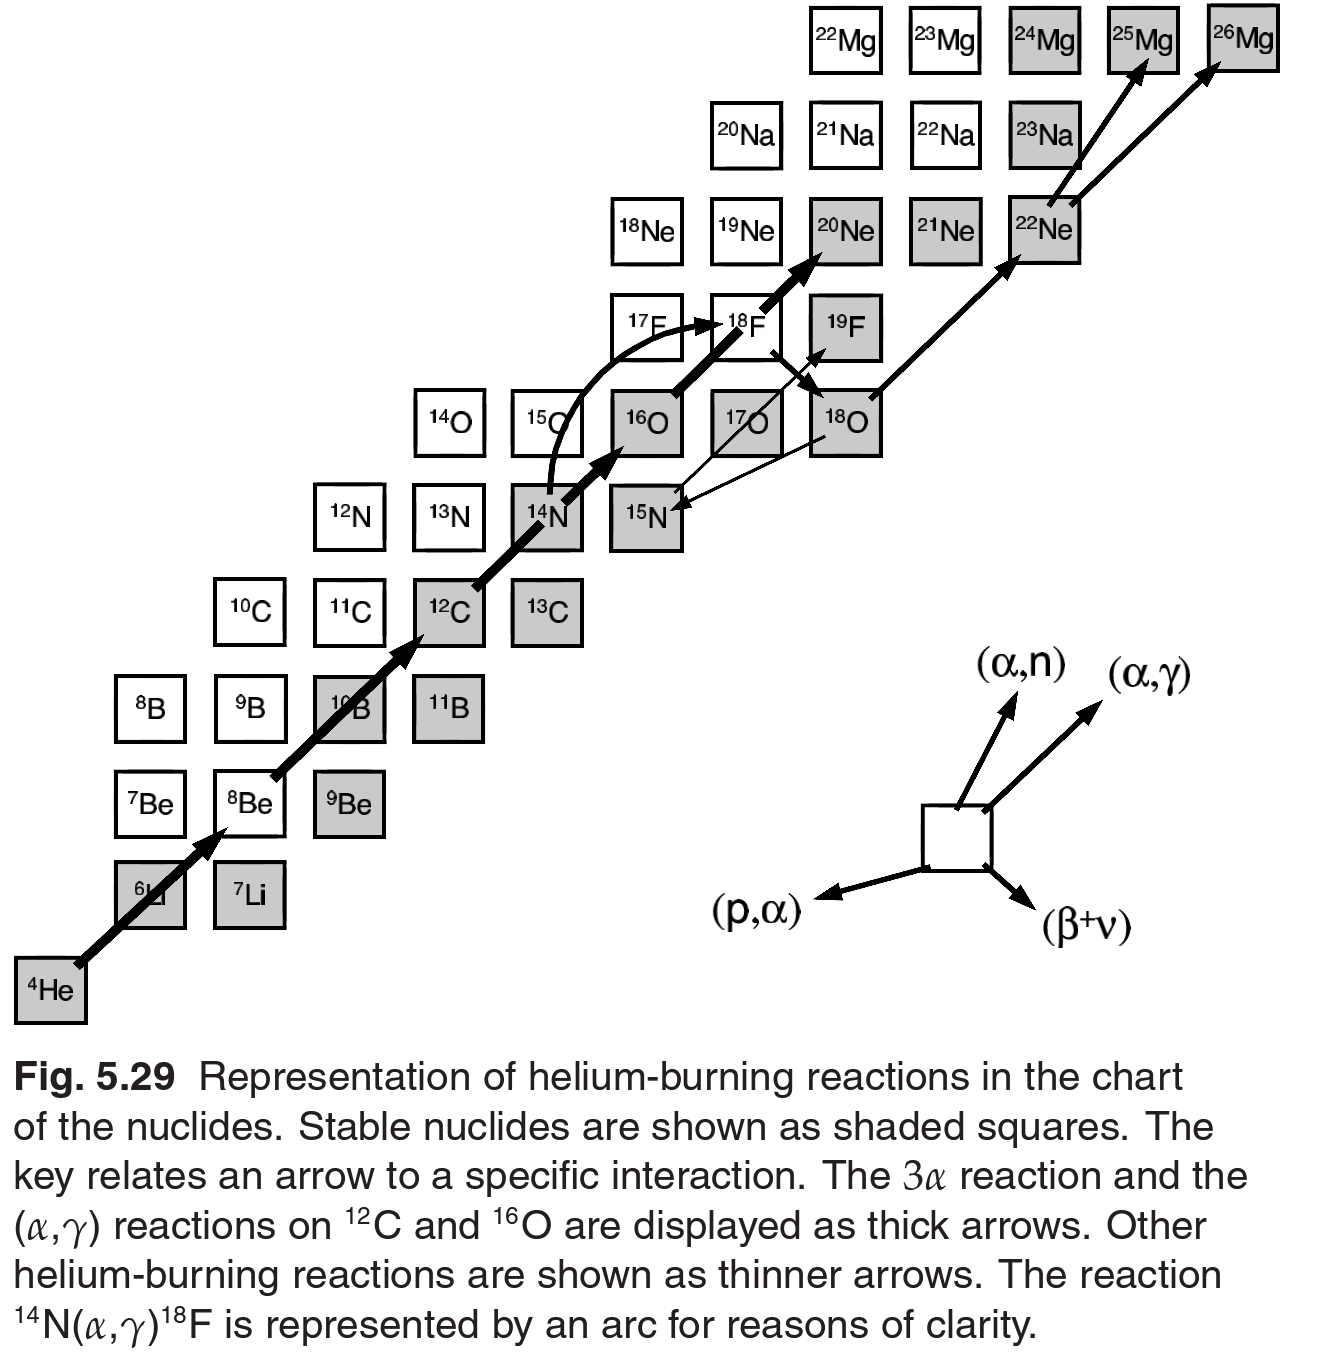
\includegraphics[trim={0cm 0cm 1cm 0cm},clip, keepaspectratio,height=0.28\textheight]{Heburningelems}
			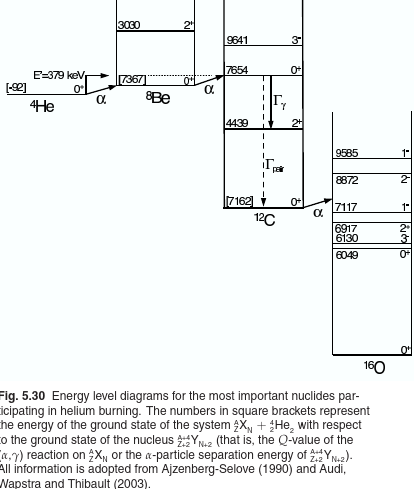
\includegraphics[trim={0cm 0cm 1cm 0cm},clip, keepaspectratio,height=0.28\textheight]{3alphalevels}
		\end{figure}
	\end{column}
\end{columns}
\end{frame}


\begin{frame}{Produzione nuclei fino al Fe56}
3$\alpha$: $He4+\alpha\to C12$, $C12+\alpha\to O16$
Produzione neutroni liberi
Fusione $C12$, fotodisintegrzione $Ne20$, fusione $O16$, fotodisintegrzione $Si28$, catture $\alpha$ su nuclei fino a produzione $Fe56$
\end{frame}

\begin{frame}{Cattura neutronica: processi r e s}
picchi r e s nella nella curva universale delle abbondanze
\end{frame}

\begin{frame}{Nuclear burning efficiency}
\begin{equation*}
\epsilon_{ij}(\rho,T,X_i)=Q_{ij}\frac{n_in_j}{\rho(1+\delta_{ij})}\lambda_{ij}=\frac{1}{1+\delta_{ij}}Q_{ij}\frac{\rho N_A^2X_jX_k}{{A_iA_j}}\exv{\sigma v}_{ij}
\end{equation*}
dove $Q_{ij}$ \'e l'energia liberata per reazione tra nucleo di specie i e j e $\exv{\sigma v}_{ij}$ \'e il rate di reazione per coppia di particelle; $X_i$ indica la frazione in  massa della specie i
\begin{columns}[T]
	\begin{column}{0.5\textwidth}
		\begin{align*}
		&PP\ \exv{\sigma v}\propto T\expy{3.9}\ E_C=\SI{0.55}{\mega\ev}\\
		&P^{14}N\ \exv{\sigma v}\propto T\expy{20}\ E_C=\SI{2.27}{\mega\ev}\\
		&\alpha+^{12}C\ \exv{\sigma v}\propto T\expy{42}\ E_C=\SI{3.43}{\mega\ev}\\
		&^{16}O+^{16}O\ \exv{\sigma v}\propto T\expy{182}\ E_C=\SI{14.07}{\mega\ev}
		\end{align*}
	\end{column}
	\begin{column}{0.5\textwidth}
		\begin{align*}
		&E_C\approx Z_1Z_2\si{\mega\ev}
		\end{align*}
	\end{column}
\end{columns}
\end{frame}

\section{Ordini di grandezza}

\begin{frame}{Energia interna}
\begin{equation*}
E_i=\int_0^Mu\,dm=\frac{3}{2}\int_M\frac{P}{\rho}\,dm\label{eq:traslintenergy}
\end{equation*}
\end{frame}

\section{Metodi per integrazione equazioni di struttura e raccordo con modelli dell'atmosfera stellare}\linkdest{nummod}

\subsection{4 Structure ODE with boundary conditions}\linkdest{fourODE}

\begin{frame}{Equazioni struttura di equilibrio}
\begin{align*}
&\TDy{m}{r}=\frac{1}{4\pi r^2\rho}\\
&\TDy{m}{P}=-\frac{Gm}{4\pi r^4}\overbrace{[-\frac{1}{4\pi r^2}\PtwoDy{t}{r}]}^{\tau_{hyd}}\\
&\TDy{m}{T}=-\nabla\frac{T}{p}\frac{Gm}{4\pi r^4}\\
&\TDy{m}{L}=\epsilon-\epsilon_{\nu} \underbrace{-c_P[\TDy{t}{T}-\nad\frac{T}{P}\TDy{t}{P}]}_{-c_P\PDy{t}{T}+\frac{\delta}{\rho}\PDy{t}{P}: \tkh}\\
&\TDy{t}{X_s}\frac{1}{A_s}=\sum_{production}\rho^{n_h+n_k-1}n_p\frac{X_h^{n_h}X_k^{n_k}}{A_h^{n_h}A_k^{n_k}}\frac{\exv{\sigma v}_{hk}}{m_H^{n_h+n_k-1}n_h!n_k!}\\
&-\sum_{distruction}\rho^{n_d+n_j-1}n_d\frac{X_s^{n_d}X_j^{n_j}}{A_s^{n_d}A_j^{n_j}}\frac{\exv{\sigma v}_{sj}}{m_H^{n_d+n_j-1}n_d!n_j!}
\end{align*}
\end{frame}

\begin{frame}{Equazioni struttura di equilibrio: condizioni al bordo}
\begin{itemize}
\item Le 4+I equazioni determinano $r$, $P$, $T$, $L$, $X_s$ specificata la massa e composizione iniziale (omogenea)
\item $\tau_n\gg\tkh\gg\tau_{dyn}$: solve 4 structure equations at time t - do time step $\Delta t$ and determine new composition - solve structure at $t+\Delta t$ with new composition
\item Solution of 4 structure equations require 4 boundary condition: 2 at surface (atmospere model without diffusion approx, PP geometry), parametri $\rho_c,T_c$; 2 at center (via Taylor expansion for $m=m'$)
\end{itemize}
\begin{columns}[T]
\begin{column}{0.65\textwidth}
\begin{align*}
&r=(\frac{3}{4\pi\rho_c})\expy{1/3}{m'}\expy{1/3}\\
&P=P_c-\frac{3G}{8\pi}(\frac{4\pi\rho_c}{3})\expy{4/3}{m'}\expy{2/3}\\
&L=\epsilon_cm'\\
&T^4=T_c^4-\frac{1}{2ac}(\frac{3}{4\pi})\expy{2/3}\kappa_c\epsilon_c\rho_c\expy{4/3}{m'}\expy{2/3}\tag*{rad}\\
&\ln{T}=\ln{T_c}-(\frac{\pi}{6})\expy{1/3}G\frac{{\nad}_c\rho_c\expy{4/3}}{P_c}{m'}\expy{2/3}\tag*{con}
\end{align*}
\end{column}
\begin{column}{0.35\textwidth}
At surface $m=M$, $L=L_s$, atmospheric model for $P$, $T$ - atmosphere defined by $g=\frac{GM}{R^2}$, $T_e$, composition: provides $P_s$ at $\tau$ where diffusion approx. starts to be valid
\end{column}
\end{columns}
\end{frame}

\begin{frame}{Simplified atmosferic model: grey atmosphere}
Atmosphere model: usually PP geometry and solve HE equation using non grey radiative transport and EOS and convection if needed
\begin{align*}
&\TDy{\tau}{P}=\frac{g}{\kappa}\tag*{HE using $\tau$ as indip var}\\
&T^4=\frac{3}{4}T_e^4(\tau+\frac{2}{3})\tag*{or solar $T(\tau)$ empirical relation}
\end{align*}
integration from $\tau\approx0$ where $T\approx0$, $P\approx0$ down to $\tau=\frac{2}{3}$ where $T=T_e$ - using shooting method.
\end{frame}

\begin{frame}{Chemical mixing: diffusion and convection}

\end{frame}

\subsection{Metodo di Henyey: modelli evolutivi}

\begin{frame}{Metodo di Henyey $[96]$}
N mass-shell with boundaries at $m_j$ $m_1=0,m_2=m',\ldots,m_N=M$
\begin{columns}[T]
\begin{column}{0.5\textwidth}
\begin{align*}
&\frac{r_{j+1}-r_j}{m_{j+1}-m_j}=\frac{1}{4\pi r_{j+1/2}^2\rho_{j+1/2}}\\
&\frac{P_{j+1}-P_j}{m_{j+1}-m_j}=-\frac{Gm_{j+1/2}}{4\pi r_{j+1/2}}\\
&\frac{L_{j+1}-L_j}{m_{j+1}-m_j}=\epsilon_n(T_{j+1/2},\rho_{j+1/2},X_{s,j+1/2})+!!!\\
&\frac{T_{j+1}-T_j}{m_{j+1}-m_j}=-\frac{T_{j+1/2}}{P_{j+1/2}}\nabla_{j+1/2}\frac{Gm_{j+1/2}}{4\pi r^4_{j+1/2}}
\end{align*}
\end{column}
\begin{column}{0.5\textwidth}
\begin{align*}
&(Y^1=r, y^2=P, y^3=T, y^4=L)\\
&E_j^{i=1,\ldots,4}=\frac{y_{j+1}^i-y^i_j}{m_{j+1}^i-m^i_j}\\
&-f_i(y_{j+1/2}^1,\ldots,y_{j+1/2}^4)=0
\end{align*}
$j=2,\ldots,N-2$: 4N-8 vincoli e le condizioni al bordo
\begin{align*}
&J=N: S_1=y_N^2-f_S(y_N^1,y_N^4)=0\\
&S_2:y^3_N-g_S(y_N^1,y_N^4)=0\\
&j=1: C_i(y^1_2,y_2^2,y_2^3,y_2^4,y_1^2,y_1^3)=0\\
&y_1^1=y_1^4=0
\end{align*}
\end{column}
\end{columns}
$4N-2$ equazioni in $4N-2$ incognite
\end{frame}

\begin{frame}{Metodo di Henyey: solve system of algebraic equations}
\'A la Newton-Rapshon - Trial solution (solution at step $t-\Delta t$): $(S_i)_1\neq0$, $(C_i)_1\neq0$, $(E_i^j)_1\neq0$ so we have to find correction to trial solution $(y_i^j)_2=(y_i^j)_1+\delta y_i^j$ - by Taylor expansion we can express $\delta S_i$, $\delta C_i$, $\delta E^i_j$ as function of the unknown small correction:
\begin{align*}
&(S_i)_1+\delta S_i=0, (C_i)_1+\delta C_i=0, (E_i^j)_1+\delta E_i^j=0\\
&\left\{\begin{array}{l}\TDy{y_N^1}{S_i}\delta y_N^1+\TDy{y_N^2}{S_i}\delta y_N^2+\TDy{y_N^3}{S_i}\delta y_N^3+\TDy{y_N^4}{S_i}\delta y_N^4=-(S_i)_1\\
\TDy{y_2^1}{C_i}\delta y_2^1+\ldots+\TDy{y_2^4}{C_i}\delta y_2^4+\TDy{y_1^2}{C_i}\delta y_1^2+\TDy{y_1^3}{C_i}\delta y_1^3=-(C_i)_1\\
\TDy{y_j^1}{E_j^i}\delta y_j^1+\ldots+\TDy{y_j^4}{E_j^i}\delta y_j^4+\TDy{y_{j+1}^1}{E_j^i}\delta y_{j+1}^1\ldots+\TDy{y_{j+1}^4}{E_j^i}\delta y_{j+1}^4=-(E_j^i)_1\\
\end{array}\right.
\end{align*}
con $i=1,\ldots,4$, $j=2,\ldots,N$: sistema algebrico di $4N-2$ equazioni in $4N-2$ $\delta y_j^i$ incognite ha matrice dei coefficienti (\keyword{Henyey matrix}) non-zero only near the diagonal e determinante non nullo - soluzione con metodi algebrici standard - fisso $\epsilon>0$ accuratezza con cui voglio risolvere le equazioni della struttura stellare e ripeto la procedura finch\'e $S_i<\epsilon$, $C_i<\epsilon$ - local errors doesn't propagate to other mesh
\end{frame}

\subsection{Metodo di shooting: soluzione primo modello stellare con condizioni al bordo}\linkdest{shooting}

\begin{frame}{Step temporale e problema modello iniziale}
Step temporale $\Delta t$: uso metodo di Henyey per determinare le nuove abbondanze with I equations as I elements accounted for.
\keyword{Problem of first model}: i) Turn on $\epsilon_g$ within few models ii) Initial model of evolutionary sequence is evaluated with \keyword{shooting method}
starting from outer mesh with 4 boundary conditions for $T_e$, $L_s$, $P_s$, $R$ and using first order approx. $y_j^i=y_{j\pm1}^i+\TDy{m}{y_{j\pm1}}\,dm$: we determine $(y_f^i)_{surf}$ until some mesh f midway between center and surface and then integrate from centerup to $j=f$ using central trial conditions - we have $(y_f^i)_{center}\neq(y_f^i)_{surf}$ and have to correct trial central boundary conditions
\begin{columns}[T]
	\begin{column}{0.5\textwidth}
\begin{align*}
&\Delta(y_f^i)_{surf}=\TDy{y_N^1}{(y^i_f)_{surf}}\delta y_N^1+\TDy{y_N^4}{(y^i_f)_{surf}}\delta y_N^4\\
&\Delta(y_f^i)_{center}=\TDy{y_1^2}{(y^i_f)_{center}}\delta y_1^2+\TDy{y_1^3}{(y^i_f)_{center}}\delta y_1^3
\end{align*}
	\end{column}
	\begin{column}{0.5\textwidth}
correzione ai 4 valori al contorno $\delta y_N^1=\delta R$, $\delta y_N^4=\delta L_s$ e $\delta y_1^2=P_c$, $\delta y_1^3=T_c$ found solving \[-\Delta_f=\Delta(y_f^i)_{center}-\Delta(y_f^i)_{surf}\]
	\end{column}
\end{columns}
Fails in advanced stages when structure has strong gradient - In massive stars late phases we can't ignore acceleration term
\end{frame}
%! TEX root = main.tex
\section{Star formation and pre MS}\linkdest{starformation}

\begin{wordonframe}{da fare/ref}
\begin{itemize}
    \item SIS: shu 1977
    \item Rev Larson 2003: The physics of star formation
    \item Evans 1999 - Physical Conditions in Regions of Star Formation
    \item Bate 2011 - Collapse of a molecular cloud core to stellar densities: the formation and evolution of pre-stellar discs
    \item Onset of star formation: kippenhahn wiegert 248'-255' (131-134) -26.1: isothermal plane parallel and spherical object in HE
    \item Formation of protostars: kippenhahn wiegert 256'-265' (135-139)
    \item Star formation and early evolution: salaris cassisi 105' (119)
        \item Stahler chap 9: Cloud equilibrium and stability
\end{itemize}
\end{wordonframe}


\begin{frame}[allowframebreaks]{List of things}
%\printbibliography[keyword={inference},heading=beamer]
%\printbibliography[keyword={\mybibcat},heading=beamer]
%\listofkeywords
\listoftodos
\end{frame}

\subsection{Clouds Properties}

\begin{frame}{Clouds Zoology}
    \begin{columns}[T]
        \begin{column}{0.4\textwidth}
            \begin{itemize}
                \item Clouds: contains $80\%$ MW's $H_2$ (\num{2e9}$\msun{}$ in galactic disk): $3\%$ converted into stars, $\tau\approx\SI{3e7}{\year}$, MW's star formation rate now $4\msun{}\si{\per\year}$
                    \item Collapse of dense core into protostars: Ambipolar diffusion, inside-out collapse, magnetized infall, Rotational effects
                \end{itemize}
        \end{column}
        \begin{column}{0.6\textwidth}
\begin{figure}[!ht]
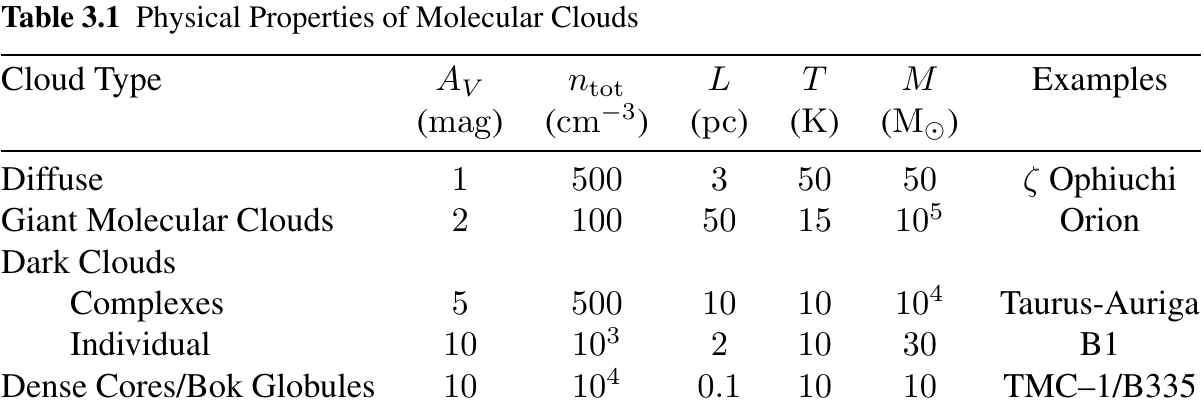
\includegraphics[trim={0cm 0cm 0cm 0cm},clip, keepaspectratio,width=0.8\textwidth]{cloudsprops}\label{fig:cloudsprops}
\end{figure}
        \end{column}
    \end{columns}
    \begin{itemize}
                    \item OB-association are correlated to giant molecular clouds: observations in \SI{2.6}{\milli\meter} of $^{12}C^{16}O$  - $^{13}C^{16}O$ lines to probe interior 
                    \item GMC are composed by clumps - clump (mass: $250\msun{}$,radius: \SI{1.5}{\parsec}, num dens: \SI{550}{\per\cubic\cm} ) - clump mass distro: $N=N_0(\frac{M}{M_{min}})^{-1.5}$, for $M>M_{min}\approx30\msun$. Smallest entities: dense cores and Bok globules (harbour infrared sources: star formation).
                    \item Extended massive atomic H envelope: comparable mass of enclosed complex, several times its linear size. Observations: excess \SI{21}{\cm} line, $T\approx$\SIrange{50}{150}{\kelvin}.
                    \item Virial-T: $\frac{1}{2}\TtwoDy{t}{I}=2T+2U+W+M$ - moment of inertia $I=\int\rho|\vec{r}|^2\,d^3r$, total kin energy $T=\frac{1}{2}\int\rho|\vec{u}|^2\,d^3x$, total thermal energy $U=\frac{3}{2}\int nKT\,d^3x=\frac{3}{2}\int P\,d^3r$, gravitational potential energy $W=\frac{1}{2}\int\rho\phi_g\,d^3x$, Magnetic Energy $M=\frac{1}{8\pi}\int|\vec{B}|^2\,d^3x$.
        \end{itemize}
Free-fall time:
\begin{align*}
&R=L/2, W\approx-\frac{GM^2}{R}, \frac{1}{2}\TtwoDy{t}{I}\approx-\frac{GM^2}{R}\\
&I\approx MR^2\Rightarrow t_{ff}\approx(\frac{R^3}{GM})^{1/2}\approx\SI{7e6}{\year}(\frac{M}{\num{e5}\msun{}})^{-1/2}(\frac{R}{\SI{25}{\parsec}})^{3/2}\\
&\rho=\frac{M}{R^3}: t_{ff}\approx(\frac{3\pi}{32G\rho})^{-\frac{1}{2}}: \tau_{MC}\approx\tau_{ff}
\end{align*}
\end{frame}

\begin{frame}{Support of giant complexes: force balance $2T+2U+W+M=0$}
    \begin{itemize}
        \item Thermal pressure $U\approx \frac{MRT}{\mu}$: $\frac{U}{|W|}\approx \frac{MRT}{\mu}(\frac{GM^2}{R})^{-1}=\num{3e-3}(\frac{M}{\num{e5}\msun{}})^{-1}(\frac{R}{\SI{25}{\parsec}})(\frac{T}{\SI{15}{\kelvin}})$ - Giant complexes not sustained by thermal pressure
        \item Magnetic field (Zeeman split of HI \SI{21}{\cm} or OH \SI{18}{\cm} lines): $\frac{M}{|W|}=\frac{|B|^2R^3}{6\pi}(\frac{GM^2}{R})^{-1}=0.3(\frac{B}{\SI{20}{\micro\gauss}})^2(\frac{R}{\SI{25}{\parsec}})^4$ - any selfgrav. mainly supported by ordered magneti field settles into planar config. BUT this is in contrast with obs. - random component of $\vec{B}$ coexistin with smooth background: MHD can provide isotropic support preventin flattening.
        \item Kin. ener. from random motion of clumps: $\frac{T}{|W|}=\frac{1}{2}M\Delta V^2(\frac{GM^2}{R})^{-1}=0.5(\frac{\Delta V}{\SI{4}{\kilo\meter\per\second}})^2(\frac{M}{\num{e5}\msun{}})^{-1}(\frac{R}{\SI{25}{\parsec}})$ - Rosetta line-of-sight dispersion is \SI{2.3}{\kilo\meter\per\second}, multiplied by $\sqrt{3}$ for random 3D velocity field, gives $\Delta V\approx V_{vir}=\sqrt{\frac{GM}{R}}$ (speed of gas parcel traversin cloud in $t_{ff}$).
        \item Line broadening: Thermal and bulk motion of emitting gas. Larson's law: $\Delta V=\Delta V_0(\frac{L}{L_0})^n$, $\Delta V_0\approx\SI{1}{\kilo\meter\per\second}$, $L_0=\SI{1}{\parsec}$, $n\approx0.5$
        \end{itemize}
\end{frame}

\begin{frame}{Birthline}
    \begin{columns}[T]
        \begin{column}{0.6\textwidth}
    \begin{itemize}
        \item Accreting stars: as gas falls onto star it lower potential energy onto the star $\Delta W\approx -\frac{GM_*\Delta m}{R}$, and gas brings its internal energy $\Delta U=\epsilon\frac{GM_*\Delta M}{R}$, $\epsilon=1$: all energy converted into heat, $\epsilon<1$: bound orbit, $\epsilon=0$: gas tot cold
        \item Birthline is locus in HDR of pre-MS stars with protostellar radius: surface L and $T_e$ are set by infalling dynamics, R is determined by internal structure
        \end{itemize}
        \end{column}
        \begin{column}{0.4\textwidth}
            \begin{align*}
                &\tkh{}=\frac{GM_*^2}{RL}: \dot{R}_*=-n_1 \frac{R_*}{\tkh{}}\\
                &L=4\pi R_*^2\sigma T_e^4: \dot{L}_*=-n_2 \frac{L_*}{\tkh{}}\\
                &\Rightarrow\tkh{}\propto L_*^{-3/2}\tag{fixed mass}
            \end{align*}
        \end{column}
    \end{columns}
\end{frame}

\begin{frame}{Isothermal clouds: Density Structure}
    \begin{align*}
        &-\frac{1}{\rho}\nabla P-\nabla\phi_g=0, P=\rho a_T^2\Rightarrow \ln{\rho}+\frac{\phi_g}{a_T^2}=\const{}: \rho(r)=\rho_c\exp{-\frac{\phi_g}{a_T^2}}\tag{Spherical}\\
        &\nabla^2\phi_g=4\pi G\rho\Rightarrow \frac{1}{r^2}\TDof{r}(r^2\TDy{r}{\phi_g})=4\pi G\rho=4\pi G\rho_c\exp{-\frac{\phi_g}{a_T^2}}\\
        &\frac{1}{\xi^2}\TDof{\xi}(\xi^2\TDy{\xi}{\psi})=\exp{-\psi},\xi=\sqrt{\frac{4\pi G\rho_c}{a_T^2}}r,\psi=\frac{\phi_g}{a_T^2}\tag{isothermal Lane-Emden}\\
        &\psi(0)=0,\psi'(\xi)\xrightarrow{\xi\to0}0\tag{Boundary conditions}\\
        &\frac{\rho}{\rho_c}\to\frac{2}{\xi^2}\Rightarrow\psi=\ln{\frac{\xi^2}{2}}, \rho(r)=\frac{a_T^2}{2\pi Gr^2}\tag{SIS: not satisfy conditions at 0 - large distance}\\
        &\rho_0=\frac{P_0}{a_T^2},r_0=\frac{\xi_0}{\sqrt{\frac{4\pi G\rho_c}{a_T^2}}}\tag{Specifying $P_0$,$a_T$ - $\frac{\rho_c}{\rho_0}$ gives non-dim radius $\xi_0$}\\
        &M=4\pi\int_0^{r_0}\rho r^2\,dr=4\pi\rho_c(\frac{a_T^2}{4\pi G\rho_c})^{\frac{3}{2}}\int_0^{\xi_0}\exp{-\psi}\xi^2\,d\xi,m=\frac{P_0^{\frac{1}{2}}G^{\frac{3}{2}}M}{a_T^4}=(4\pi \frac{\rho_c}{\rho_0})^{-\frac{1}{2}}(\xi^2\TDy{\xi}{\psi})_{\xi_0}
        \end{align*}
        At beginning sequence $\frac{\rho_c}{\rho_0}=1$: $\xi_0=0$, $m=0$; with increasing density contrast m first rises to maximum $m_1=1.18$ at $\frac{\rho_c}{\rho_0}=14.1$, then decreses to minimum $m_2=0.695$, eventually approachin to $m_{\infty}=\sqrt{\frac{2}{\pi}}=0.798$: non dimensional mass of SIS.
    \end{frame}

    \begin{frame}{Gravitational stability of SIS}
        \begin{align*}
            &m=\frac{P_0^{\frac{1}{2}}G^{\frac{3}{2}}M}{a_T^4}: \xincreases{P_0},\xincreases{m}\Rightarrow\xincreases{\frac{\rho_c}{\rho_0}}(\xincreases{\xi_0})\Rightarrow \xincreases{P_c},\xincreases{\exv{P}}\tag{M fixed, $a_t$ fixed, low $\rho$ contrast, $\frac{\rho_c}{\rho_0}<14.1$}\\
            &M_{BE}=\frac{m_1a_T^4}{P_0^{\frac{1}{2}}G^{\frac{3}{2}}}\tag{For $\frac{\rho_c}{\rho_0}>14.1$ instability - critical value $M_{BE}$ where fundamental modes becomes unstab.}\\
            &\psi(\xi)=\exp{-\psi}\approx1-\frac{\xi_0^2}{6}\tag{Small $\xi$: $\psi(\xi)=\frac{\xi^2}{6}+O(\xi^4)$ - Density contrast for cloud of nonDim radius $\xi_0$}\\
            &m=(4\pi \frac{\rho_c}{\rho_0})^{-\frac{1}{2}}(\xi^2\TDy{\xi}{\psi})_{\xi_0}: M\approx \frac{\xi_0^3}{6\pi^{\frac{3}{2}}}\frac{a_T^4}{P_0^{\frac{1}{2}}G^{\frac{3}{2}}}\tag{DenseCore, BokGlobule are on edge of g.i.}\\
            &\xi=\sqrt{\frac{4\pi G\rho_c}{a_T^2}}r,\xi_0=\sqrt{\frac{4\pi G\rho_c}{a_T^2}}r_0: \xi_0^3=(4\pi)^{\frac{3}{2}}(\frac{\rho_c}{\rho_0})^{\frac{3}{2}}\frac{P_0^{\frac{3}{2}}G^{\frac{3}{2}}}{a_T^6}\tag{$\frac{\rho_c}{\rho_0}\approx1$}\\
            &\Rightarrow r_0^3\approx\frac{3Ma_T^2}{4\pi P_0},\xdecreases{r_0},\xincreases{P_0},P_0\frac{4\pi r_0^3}{3}\approx\const{}\tag{Boyle's law}\\
            &\rho(x,t)=\rho_0+\delta\exp{i(kx-\omega t)},\rho \frac{D\vec{u}}{Dt}=\rho[\TDy{t}{\vec{u}}+\scap{u}{\nabla}\vec{u}]=-\nabla P-\rho\nabla\phi_g\tag{stability against linear perturb}\\
            &-i\omega\delta\rho+ik\rho_0\delta u=0\tag{cont}\\
            &\delta P=\delta\rho a_T^2\tag{EOS}\\
            &-k^2\delta\phi_g=4\pi G\delta\rho\tag{Poiss.}\\
            &-i\omega\rho_0\delta u=-ik\delta P-ik\rho_0\delta\phi_g\tag{EOM}\\
            &\Rightarrow-\omega^2\delta\rho=-k^2\delta P-k^2\rho_0\delta\phi_g=-k^2a_T^2\delta\rho-k^2\rho_0\delta\phi_g\Rightarrow\omega^2=k^2a_T^2-4\pi G\rho_0\tag{dispersion relation}\\
            &\lambda_J=\sqrt{\frac{\pi a_T^2}{G\rho_0}}=\SI{0.19}{\parsec}\sqrt{\frac{T}{\SI{10}{\kelvin}}}(\frac{n_{H_2}}{\SI{e4}{\per\cubic\cm}})^{-\frac{1}{2}}, M_{BE}=M_J=\frac{m_1a_T^3}{\rho_0^{\frac{1}{2}}G^{\frac{3}{2}}}=1\msun{}(\frac{T}{\SI{10}{\kelvin}})^{\frac{3}{2}}(\frac{n_{H_2}}{\SI{e4}{\per\cubic\cm}})^{-\frac{1}{2}}
        \end{align*}
        Perturbation with $\lambda>\lambda_J$ grow exponentially: uniform sphere of diameter $\lambda_J$ has mass $2M_{BE}$.
    \end{frame}

\subsection{From clouds to proto-stars}\linkdest{protostellar}

\begin{frame}{Molecular Clouds: density and clumps formation}
\begin{itemize}
        \item Calculations: small fraction of collapsing cloud core attains density to form a star; in SIS model envelope is at rest instead of falling at approx twice $c_s$ as in dynamical collapse.
\item clouds equilibrium shape: Observed cloud mass greater than Jeans mass; Rotation and magnetic field support increases Jeans mass
\item $H_2$ molecules formation: dust grains enhance $H_2$ formation which increases with density and column density of at least $20\msun{}\si{\per\square\parsec}$ (Column density: Mangum shirley 2015) is required to shield from UV, where typical column density is $100\msun\si{\per\square\parsec}$ (Elmegreen 85, 93); column density of cold $H_2$ is hard to measure directly infact is measured indirectly by collisional excitation of other molecules and by relative decrese of 21-cm emission/absorption line strenght from deplition of atomic H. ($\msun/pc^2\approx 2*10^{-4}gr/cm^2$).
\item Collisional excitation cooling by molecular/atomic lines emission increases with density while external heating decreases: MC are very cold (\SIrange{10}{20}{\kelvin}); far IR emission of CO; in densest regions gas is thermally coupled to dust mantaining $T\approx10K$.
\item Inefficient conversion of MC into stars: turbulence, magnetic fields.
\item Almost all MC are star forming: short lifetime, young age - $\tau_{MC}$ approx crossing time of internal turbulent motion $<\SI{1}{\mega\year}$
\item Fragmentation. Youngest stars are in denser part of MC: denser clumps may originate from Small fluctuation amplified by gravitational instabilities or Supersonic turbulent motion may compress gas into observed clumpy structure.
\item How collapse is initiated - Prestellar cloud core: Gravitational instability, for example Bonnor-Ebert sphere that slightly exceeds stability threshold, or if prestellar core are magnetically supported condensing gradually by ambipolar diffusion (neutral species collapse) whereby gas contract slowly along across field lines (SIS: singular isothermal sphere with no magnetic support $\rho(r)=\frac{c_s^2}{2\pi Gr^2}$, $M(r)=\frac{2c_s^2}{G}r$).
\end{itemize}
\end{frame}

\begin{frame}{Inside-out Spherical collapse: formation and accretion onto protostar} 
    \begin{itemize}
        \item Equilibrium model with margin-stable $M_{BE}=\frac{1.18a_T^4}{\sqrt{P_O}G^{\frac{3}{2}}}$. Transition to ff collapse $V_{ff}\approx a_T$, ie $\frac{G\dot{M}t}{R_{ff}}\approx a_T^2$, $\dot{R}_{ff}\approx \frac{R}{t}$; for $\dot{M}>0$: $\dot{R}_{ff}>0$, region of ff spreads.
        \item At low $\rho$: \xaumenta{\rho} \xdiminuisce{T} (increases atomic/molecular lines cooling); At higher $\rho$: gas becomes thermally coupled to dust which controls T with its thermal emission - T is \SIrange{6}{12}{\kelvin} while $\rho$ spans many OM as long as core remains optically thin to dust thermal radiation ($n_{H_2}<\SI{e10}{\per\cubic\cm}$).
        \item Most collapse calculation assume early stages isothermal at \SI{10}{\kelvin} (whitworth 98) and a universal result of isothermal collapse is runaway growth of central density peak (Penston 66, Bodenheimer Sweigart 68, Larson 69)
        \item In absence of pressure gradient the collapse of uniform sphere happens in $t_{ff}\approx\sqrt{\frac{3\pi}{32G\rho}}$: denser inner regions collapse faster (Larson 73, Tohline 82). Numerics show that $\rho\propto r\expy{-2}$ for collapsing isothermal sphere asymptotically for smaller radii as long as isothermal approx holds (Larson 69, Ogino 99); peak width at any stage of order of Jeans length $\propto\rho\expy{-1/2}$.
        \item Rotation. Forming cloud core rotate as expected due to turbulence in MC (Burket Bodenheimer 00) - ''Angular Momentum Problem'': much more angular momentum in MC than rotating stars - magnetic field can't dispose excess angular momentum: formation of multiple system. Narita 84: competition between pressure and gravity near center - centrifugal force never become strong enough there to halt condensation (rather the material with higher angular momentum produce a disk). Also for SIS model rotation could produce disk then spiral density fluctuation could cause inward mass transfer or disk fragmentation.
        \item Collapse with Magnetic Field. Timescale Ambipolar Diffusion \SI{e7}{\year} which is one OM greater then ff timescale; as in the central part gravity force become dominant the core becomes more flattened along field lines, when central part becomes unstable runaway collapse begins (flattened, collapse speed approx sound speed). Ambipolar Diffusion may solve ''Magnetic flux problem'' for star formation

    \end{itemize}
\end{frame}

\frameinlbftrue
\begin{frame}{Optically Thick Phase}
    \begin{itemize}
        \item Always central density peak is realize in spite of thermal pressure never being negligible near central regions; spherical symmetry at later stage when optical depth of central regions becomes large and radiative cooling unimportant and T rises (3D calculation partially support spherical Approx: Bate 98): rotational flattening may eventually becomes important and transient spiral appears (gravitational torque transfer enough angular momntum outward to allow growth of central mass.
            \item Calculation show formation of central object or protostar: Larson 69, 72, Appenzeller Tscharnuter 75, Winkler Newman 80, Masunaga Inutsuka 00 (later stages), Wuchterl Tscharnuter 03.
            \item Central regions becomes opaque for thermal radiation of dust for $\rho_c>\SI{e-13}{\gram\per\cubic\cm}$ ($\num{2e10} H_2$ \si{\per\cubic\cm}), transition to adiabatic evolution: completely adiabatic for $\rho>\SI{e-12}{\gram\per\cubic\cm}$ with ratio of specific heat $\gamma=\frac{7}{5}$ consistent for $H_2$ gas. As density continues to rise pressure increses faster than gravity and collapse halts at $\rho_c\approx\SI{2e-10}{\gram\per\cubic\cm}$: first hydrostatic core is formed with accreting shock at surface (mass $0.01 \msun{}$, radius several AU); its properties are almost indep. of initial conditions/boundary conditions due to convergence toward selfsimilar behaviour during isothermal collapse.
            \item Formation of second hydrostatic core, mass $0.001\msun{}$, radius $\rsun{}$: when $T_c>\SI{2000}{\kelvin}$ $H_2$ dissociates reducing $\gamma<\frac{4}{3}$ required for stability, hence we have a second collapse phase producing runaway central concentration; rapid collapse is halted when H is completely ionized at center and $\gamma=\frac{5}{3}$. Second hydrostatic core bounded by accretion shock.
            \item Predicted stars begins its life as small embryo $<\num{e-2}\msun{}$, the accreting surface is surrounded by optically thick materials hence the shock is adiabatic: outer layers of protostars are strongly heated and expands rapidly, until the reach $4\rsun{}$ when acreted all materials of first hydrostatic core (Masunaga Inutsuka 00).
            \item When rotation is present materials from first hydrostatic core has significant angular momentum and sets into disk (Yorke Bodenheimer 99), outward angular momentum transfer is needed to have predicted accretion rate (Mercer Smith 84).
    \end{itemize}
\end{frame}
\frameinlbffalse

\begin{frame}{Onset of cloud formation ($\tau_{ff}\gg\tau{KH}$). Jeans Criterion}
\begin{columns}[T]
\begin{column}{0.55\textwidth}
    \begin{itemize}
        \item Infinite homogeneous gas at rest: not well defined state, ie for symmetry reasons also g. potential $\phi$ must be const but from Poiss. we have $\nabla^2\phi=4\pi G\rho$ hence $\rho=0$; but if we apply periodic perturb. of suff. small wavelength the single perturbation will behave like one with same $\lambda$ in isothermal sphere at static equilibrium
        \item Gas obeys to:
\begin{align*}
    &\PDy{t}{\vec{v}}+(\vec{v}\cdot\nabla)\vec{v}=-\frac{1}{\rho}\nabla P-\nabla\phi\tag{EOM/Euler}\\
    &\PDy{t}{\rho}+\vec{v}\cdot\nabla\rho+\rho\nabla\cdot\vec{v}=0\tag{cont. eq.}\\
    &\nabla^2\phi=4\pi G\rho,\ P=\frac{R}{\mu}\rho T=v_s^2\rho\tag{Poiss.}\\
    &P=\frac{R}{\mu}\rho T=v_s^2\rho\tag{EOS}
\end{align*} 
$T=T_0=\const$, $\rho=\rho_0=\const$, $\nabla^2\phi_0=4\pi G\rho_0$
    \end{itemize}
\end{column}
\begin{column}{0.45\textwidth}
    \begin{itemize}
        \item Perturbazioni:
\begin{align*}
    &\rho=\rho_0+\rho_1,P=P_0+P_1,\phi=\phi_0+\phi_1,\vec{v}=\vec{v}_1\\
&\PDy{t}{\vec{v}_1}=-\nabla(\phi_1+v_s^2\frac{\rho_1}{\rho_0})\\
&\PDy{t}{\rho_1}+\rho_0\nabla\cdot\vec{v}_1=0\\
&\nabla\phi_1=4\pi G\rho_1
\end{align*}
Homogeneous ODE system with constant coeffs.
\item Assuming isothermal pertur. ($v_s$ unperturbed) and taking only linear terms
\item Solutions prop.to $\exp{i(kx+\omega t)}$: $\PDof{x}=ik$, $\PDof{y}=\PDof{z}=0$, $\PDof{t}=i\omega$
    \end{itemize}
\end{column}
\end{columns}
\begin{columns}[T]
	\begin{column}{0.3\textwidth}
		\begin{align*}
		&\omega v_1+\frac{kv_s^2\rho_1}{\rho_0}+k\phi_1=0\\
		&k\rho_0v_1+\omega\rho_1=0\\
		&4\pi G\rho_1+k^2\phi=0
		\end{align*}
	\end{column}
	\begin{column}{0.3\textwidth}
Non trivial solution
		\begin{align*}
		&\begin{vmatrix}
            \omega&\frac{kv_s^2}{\rho_0}&k\\
		k\rho_0&\omega&0\\
		0&4\pi G&k^2\\
		\end{vmatrix}=0\\
		&\omega^2=k^2v_s^2-4\pi G\rho_0
		\end{align*}
	\end{column}
	\begin{column}{0.4\textwidth}
$k$ large: $\omega$ real (oscillations). 
\begin{align*}
    &\lambda<\lambda_J=\frac{2\pi}{k_J}=\sqrt{\frac{\pi}{G\rho_0}}v_s\tag{Stable}\\
    &k<k_J=\frac{4\pi G\rho_0}{v_s^2}\tag{Unstable}
\end{align*}
Collapsing plane-parallel slab: $i\omega\approx\sqrt{G\rho_0}$
\end{column}
\end{columns}
\end{frame}

\begin{frame}{Jeans inst ability in isothermal sphere}
    \begin{columns}[T]
        \begin{column}{0.5\textwidth}
            \begin{itemize}
                \item $P*>0$: we get the structure fro ma solution of LE equation for isothermal polytrope
                \item Virial T: Internal energy $E_i=c_VMT$, for g. energy $E_g=\Theta \frac{GM^2}{R}$ ($\Theta$ can be obtained from LE iqu.)
                \item Using  virial t. $\zeta E_i+E_h=4\pi R^3P_0$: per $\zeta=2$ si ha $P_0=\frac{c_VMT}{2\pi R^3}-\frac{\Theta GM^2}{4\pi R^4}$
                \item For small $R$ $P_0<0$, changes sign for increasing $R$, $P_0\to0$ for $R\to\infty$ and reaches a max. at $R_m$
                \item Differentiating eq for $P_0$ we found $R_M=\frac{4\Theta}{9}\frac{G\mu M}{RT}$
            \end{itemize}
        \end{column}
        \begin{column}{0.5\textwidth}
            \begin{itemize}
                \item Stab ility of LE solution - Starting at equilibrium at $P^*=P_0$: for $R<R_m$ (unstable config.) equilibrium pressure $P_0$ decreses with decreasing $R$, therefore after slight compression $P^*>P_0$ and sphere compress more, for $R>R_m$ $P_0$ (stable)increses during slight compression and sphere will expand back to equilibrium.
                \item Same as Jeans Stability crit.: $M=\frac{4\pi}{3}r_m^3\bar{\rho}$. $R_m^2=\frac{27}{16\pi\Theta}\frac{RT}{G\mu\bar{\rho}}$ where $R_m$ is critical radius of gas with mean density $\bar{\rho}$ and T which is marg. stable - comparing with critical Jeans wavelength, $\lambda_J=\sqrt{\frac{\pi} {G\rho_0}}v_s$: they are same OoM.
            \end{itemize}
        \end{column}
    \end{columns}
    Expression for critical mass (Jeans mass): $M>M_J$ are unstable:
	\begin{align*} 
        &M_J=\frac{4\pi}{3}\exv{\rho}R_m^3:\ M_J=\frac{27}{16}\sqrt{\frac{3}{\pi}}(\frac{R}{\Theta G})^{\frac{3}{2}}(\frac{T}{\mu})^{\frac{3}{2}}(\frac{1}{\exv{\rho}})^{\frac{1}{2}}\tag{Virial/LE eq}\\
&M_J=\num{1.2e5}\msun{}(\frac{T}{\SI{100}{\kelvin}})^{\frac{3}{2}}(\frac{\rho}{\SI{e-24}{\gram\per\cubic\cm}})^{-\frac{1}{2}}\mu^{-\frac{3}{2}}\tag{pertub.}
	\end{align*}
\end{frame}

\begin{frame}{Jeans Mass and collapse: $-\frac{1}{2}E_g>E_k$. End free-fall phase}
    \begin{itemize}
        \item $E_k=\frac{3}{2}KT \frac{M}{\mu m_H}$, $E_g-\int_0^M \frac{Gm}{r}\,dm=-\frac{3}{5}$\frac{GM^2}{R}$: gravity wins if $-E_g>E_k$. This is the case when $\frac{3KT}{2\mu m_H}M>\frac{3}{10}\frac{GM^2}{R}$, ie when $M>M_J=\frac{5KT}{\mu m_H}\frac{R}{G}\approx100\sqrt{\frac{T^3}{\mu^4n}}\msun{}$.
\item Collapse trigger: i) Cloud passing density wave of a spiral arm ii)Cloud compression by shockwave of SN iii)Cloud-Cloud collision\item Free-fall timescale: $\tff{}\approx(G\rho)^{-\frac{1}{2}}\approx\num{e8}(\mu n)^{-\frac{1}{2}}\si{\year}$\
\item No cooling mechanism: adiabatic collapse $T\propto\rho^{\frac{2}{3}}$
\item cooling mechanism: i) collisions between molecules excite roto7vibro level: the molecules emit photons in IR/submm that can leave as clouds are thin in IR ii) In high density, low T cloud dust can form: collision with molecules heat the dust that emit in IR.
\item freefall ends when cooling mechanism stop working, conseq heating and hydrostic equilibrium achieved
    \item At center of clump HE is reached first while surounding keeps freefalling - The clump is the protostar
    \item Colling mechanism stop working when $H_2$ molecules dissociate, then H ionize ($\chi_{H_2}=\SI{4.5}{\ev}$, $\chi_H=\SI{13.6}{\ev}$); for cloud with $X=0.7$, $Y=0.3$:
        \begin{align*}
            &E_{dis}=\frac{MX}{m_H}[0.5\chi_{H_2}+\chi_H]=\num{1.3e58}(\frac{M}{\msun})\si{\ev}=\num{2e46}\frac{M}{\msun}\si{\erg}\\
            &\Delta E_g=AGM^2[\frac{1}{R_{end}}-\frac{1}{R_{begin}}]\approx A \frac{GM^2}{R_{end}}\approx\num{4e48}A \frac{(M/\msun{})^2}{R_{end}/\rsun{}}\si{\erg}\tag{Energy provided by contraction}
        \end{align*}
        For const density $A=\frac{3}{5}$, since now we have a concentrated object assume $A\approx2$. Cloud loses most of gained energy in far-IR photons: only a fraction $f<1$ of $\Delta E_g$ is used for diss./ion. (if clump contract quasi-hydrostatically $f\approx0.5$ according to virial, detailed calculation show that $f\approx0.3$). Equating energy needed for diss/ioniz $E_{dis}=f\Delta E_g$ we found protostar ionized when $\frac{R}{\rsun}\approx100\frac{M}{\msun{}}$
        \end{itemize}
\end{frame}

\begin{frame}{End of Fragmentation: Transition to adiabatic collapse.}
	Cooling processes: $E_g\approx\frac{GM^2}{R}$ has to be radiated at rate $A\approx\frac{GM^2}{R}(G\exv{\rho})^{\frac{1}{2}}\propto\frac{G^{\frac{3}{2}}M^{\frac{5}{2}}}{R^{\frac{5}{2}}}$; radiation emission as fraction f of radiation emitted from black body $B=4\pi f\sigma T^4R^2$
	\begin{columns}[T]
		\begin{column}{0.5\textwidth}
In isothermal collapse ($B\gg A$) $M_J\propto\rho^{-\frac{1}{2}}$ so as density increases the cloud undergoes ''sub collapses''.
		\end{column}
		\begin{column}{0.5\textwidth}
At end of isothermal collapse, when matter becomes opaque $A\approx B$, begins adiabatic collapse phase (approx thermal equilibrium):
 \begin{align*}
&\nad=\TDly{P}{T}_a=\frac{2}{5}\\
&T\propto P^{\frac{2}{5}}, P\propto\rho T:\ T\propto\rho^{\frac{2}{3}}\\
&M_J\propto T^{\frac{3}{2}}\rho^{-\frac{1}{2}}\propto\rho^{\frac{1}{2}}
 \end{align*}
		\end{column}
	\end{columns}
At end of fragmentation $M_J\approx0.02\msun{}\frac{T^{\frac{1}{4}}}{f^{\frac{1}{2}}}$
\end{frame}

\begin{frame}{Free-fall collapse of (h-)sphere. Collapse onto condensed object.}
$(\frac{g}{\nabla P})\propto\frac{M}{RT}\propto\frac{1}{R}$: collapse is more and more dominated by (g)ravitation (homologous contraction: $\frac{r}{r_0}$, $\frac{\dot{r}}{r_0}$ are same for all shell at given t)
\begin{align*}
&\ddot{r}=-\frac{Gm}{r^2}\Rightarrow\frac{1}{2}\dot{r}^2=\frac{4\pi r_0^3}{3r}G\rho_0+\const{}\\
&\frac{\dot{r}}{r}=-\sqrt{\frac{8\pi}{3}G\rho_0(\frac{r_0}{r}-1)},\cos^2{\zeta}=\frac{r}{r_0}\Rightarrow \zeta+\frac{1}{2}\sin{2\zeta}=\sqrt{\frac{8\pi G\rho_0}{3}}t
\end{align*}
When opacity gets bigger in central regions collaps stalls. $\dot{M}=4\pi r^2v\rho$ constant in space and time over central mass $M$ in HE: $\frac{2}{r}+\frac{1}{\rho}\TDy{r}{\rho}+\frac{1}{v}\TDy{r}{v}$, $v=v_{ff}=\sqrt{\frac{GM}{2r}}$ so $\frac{1}{\rho}\TDy{r}{\rho}=-\frac{3}{2r}$ ie $\rho(r)=\frac{\const{}}{r^{\frac{3}{2}}}$.

Radiation loss: $L_{accr}=\frac{1}{2}v_{ff}^2(R)\dot{M}=\frac{1}{4}\frac{GM}{R}\dot{M}$.

Collapse calculation:
\begin{align*}
&\PDy{}{}+4\pi r^2v\rho=0,\ \TDof{t}=\PDof{t}+v\PDof{r}\\
&\PDy{t}{v}+v\PDy{r}{v}+\frac{GM}{r^2}+\frac{1}{\rho}\PDy{r}{P}=0\tag{EOM}\\
&\PDy{t}{u}+P\PDof{t}(\frac{1}{\rho})+v[\PDy{r}{u}+P\PDof{r}(\frac{1}{\rho})]+\frac{1}{4\pi\rho r^2}\PDy{r}{l}=0,\ l=-\frac{16\pi acr^2}{3\kappa\rho}T^3\PDy{r}{T}
\end{align*}
\end{frame}

\begin{frame}{Optically thin phase and core formation}
\begin{columns}[T]
\begin{column}{0.55\textwidth}
\begin{itemize}
	\item Isothermal phase $T\approx\SI{10}{\kelvin}$ - when instability turns nonlinear contraction isn't homologous ($t_{ff}$ is smaller for inner shell: $\rho\propto r^{-2}$).
	\item Central region becomes opaque at $\rho\approx\SI{e-13}{\gram\per\cubic\cm}$: density increases causes adiabatic pressure increases until collapse stops.
	\item As M core increases and radius decreases v of infalling materials exeeds sound speed: shock region separating supersonic rain from hydrostatic core.
	\item Hydrostatic core: protostar - $\rho_e$, $v_e$ infalling matter then $P_i=\rho_ev_e^2=\rho_e\frac{GM}{2R}$ (momentum conservation: $P+\rho v^2$ is the same on both sides) 
\end{itemize}
\end{column}
\begin{column}{0.45\textwidth}
\begin{figure}[!ht]
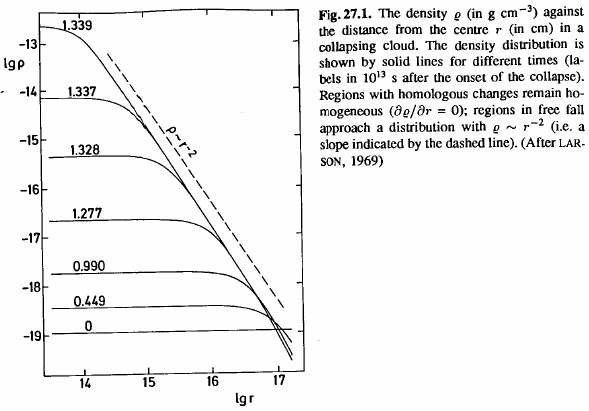
\includegraphics[trim={0cm 0cm 0cm 0cm},clip, keepaspectratio,width=0.8\textwidth]{collapsingdensity}\label{fig:collapsingdensity}
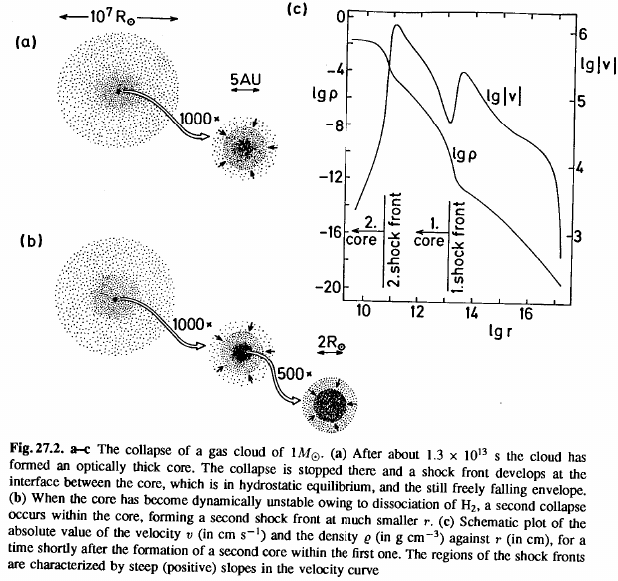
\includegraphics[trim={0cm 0cm 0cm 0cm},clip, keepaspectratio,width=0.8\textwidth]{collapsedensitystructure}\label{fig:collapsedensitystructure}
\end{figure}
\end{column}
\end{columns}
\end{frame}

\begin{frame}{core collapse}
\begin{columns}[T]
	\begin{column}{0.55\textwidth}
	\begin{itemize}
	\item For $H_2$ $\gamma_{ad}=\frac{f+2}{f}=\frac{7}{5}=1.4\approx\frac{4}{3}\approx1.33$, for $H$ $\gamma_{ad}=\frac{5}{3}\approx1.667$.  Slight decreases of $\gamma_{ad}<\frac{4}{3}$ by $H_2$ dissociation: collapse.
	\item When all hydrogen is dissociated $\gamma_{ad}>\frac{4}{3}$
	\item Central compression (of innermost core) is adiabatic as $\tau_{accr}<\tau_{KH}$, then $\dot{M}\to0$ and evolution is no more adiabatic.
	\end{itemize}
	\end{column}
	\begin{column}{0.45\textwidth}
	\begin{figure}[!ht]
	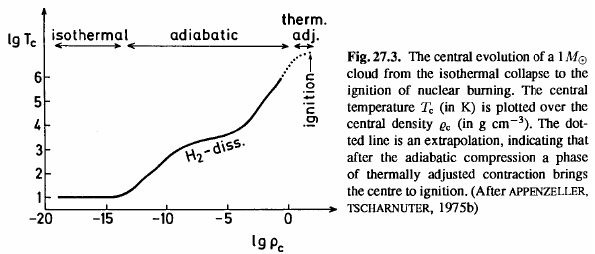
\includegraphics[trim={0cm 0cm 0cm 0cm},clip, keepaspectratio,width=0.99\textwidth]{centralcollapseevolution}\label{fig:centralcollapseevolution}
	\end{figure}
	\end{column}
\end{columns}
\begin{itemize}
    \item Mean T at end of collapse. Virial: $\frac{3}{2}\frac{M}{\mu m_H}K\bar{T}=\frac{A}{2}\frac{GM^2}{R}$ so $\bar{T}\approx \frac{A}{3}\frac{\mu m_H}{K}\frac{GM}{R}$.
    \item Star is almost completely convective: $\rho\approx\SI{e-6}{\gram\per\cubic\cm}$: at such low T and $\rho$ abs coeff is high $\kappa\approx\SIrange{e2}{e3}{\square\cm\per\gram}$.
    \end{itemize}
\end{frame}

\begin{frame}{Evolution of protostar in HR}
\begin{itemize}
\item Far from HE: radiation emitted by core is absorbed by envelope's grain and re-emitted in IR. Infalling envelope. Start on far right in HR diagram.
\item Thinning of envelope: photosphere moves downward until reaches core - $T_{ff}$ increases
\item In accretion phase $L\approx L_{accr}\propto\dot{M}$, then $L\approx L_g$ of core. Strong accretion rate heats core and make it isothermal, then a T gradient builds up and convection developes downward from surface - we found object on HL if fully convective, normal condition at border and envelope is thin in V.
\end{itemize}
\end{frame}

\subsection{Pre main sequence ed approccio a ZAMS per stelle di sequenza superiori/inferiori}\linkdest{preMS}

\begin{frame}{Traccia di Hayashi}
Primo/secondo core di Larson; Evoluzione di PMS sulla traccia di Hayashi; ruolo di opacit\'a di H- nella verticalit\'a della traccia di Hayashi; fusione deuterio; stelle completamente convettive o con nucleo radiativo. Abbondanza elementi leggeri in stelle di pre-sequenza
\end{frame}


\begin{frame}{Jeans mass ($\num{e5}\msun$)}
\todo{Instability} $\omega^2=k^2c_s^2-4\pi G\rho<0$:
\[\lambda>\lambda_H=\sqrt{\frac{\pi c_s^2}{G\rho}}=\SI{0.19}{\parsec}\sqrt{\frac{T}{\SI{10}{\kelvin}}}(\frac{n_{H^2}}{\SI{e4}{\per\cubic\cm}})\expy{-1/2}\]
\end{frame}

\begin{frame}{Protostar: first core and main accretion}
Virial T. $2E_i+\Omega=0$: $3kT\frac{M}{\mu m_H}=\int_0^M\frac{Gm}{r}\,dm$: collapse $\frac{3kTM}{\mu m_H}<\frac{3}{5}\frac{GM^2}{R}$ - $M>M_J=(\frac{3}{4\pi\rho})\expy{1/2}(\frac{5kT}{G\mu m_H})\expy{3/2}\propto T\expy{\frac{3}{2}}\rho\expy{-\frac{1}{2}}$
$t_{ff}\approx(G\rho)\expy{-\frac{1}{2}}\ll t_{cool}$: collasso adiabatico $P\propto T\expy{5/2}$ ($PT\expy{\frac{\gamma}{1-\gamma}}$) - $t_{ff}\gg t_{cool}$: collasso isotermo - \keyword{fragmentation}: Hydrostatic core surrounded by ff gas ($0.01\msun$) \todo{star formation hydrostatic core}
\end{frame}

%! TEX root = main.tex
\section{Evoluzione stellare}\linkdest{stellarevolution}

\subsection{Pre-MS}

\begin{wordonframe}{da fare: kippenhahn wiegert}
	\begin{itemize}
		\item Hayashi line 224'-232' (119-123)
		\item pre-main sequence contraction 266'-270' (140-142)
	\end{itemize}
\end{wordonframe}

\begin{frame}{Traccia d'Hayashi: protostar can be described by SSE}
	\begin{columns}[T]
		\begin{column}{0.50\textwidth}
            \begin{figure}[!ht]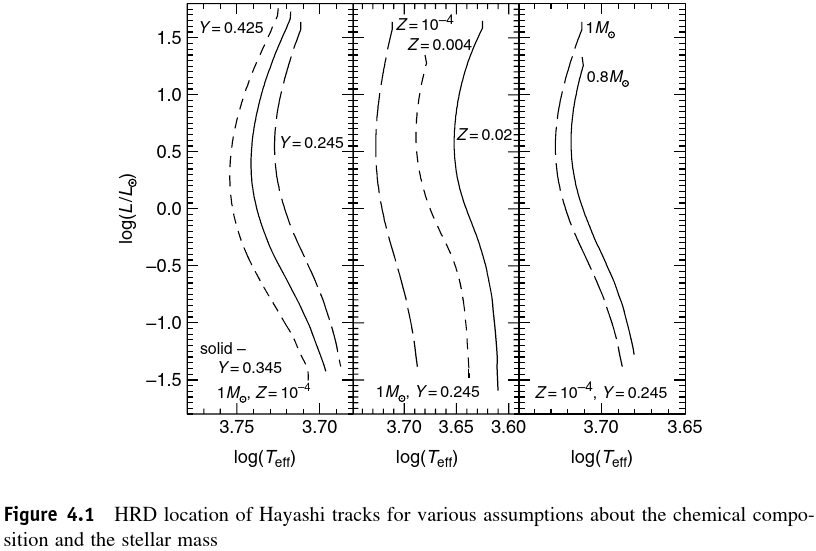
\includegraphics[trim={0.6cm 0cm 1.1cm 0},clip, keepaspectratio,width=0.95\textwidth]{hayatrack}
			\end{figure}
		\end{column}
		\begin{column}{0.50\textwidth}
            \begin{itemize}
                    \item $\log{T_e}=A\log{L}+B\log{M}+\const{}$: $\TDly{T_e}{L}=\frac{1}{A}\gg1$ HL almost vertical, HL shift to left as \xaumenta{M}.
                    \item Extension of superadiabatic layer and ionization zones varies with $L$: $A>0$ for low L and changes sign at $L\approx\lsun$: see effects of superadiabatic convection and depression of $\nabla_{Ad}$ in next.
                    \item Fully convective star model as contracting polytrope with no nuclear source, $n=\frac{1}{\nabla_{Ad}}-1=\frac{3}{2}$, $P=CT^{n+1}$: on HL $\exv{\nabla}=\nabla_{Ad}$, close to HL $\exv{\nabla}=\invers{(1+n)}$, $\PDy{n}{\log{T_e}}>0$ star move to right as $n$ decreases ($\exv{\nabla}$ increases, in a model to the left of HL the radiative part decreases average value $\exv{\nabla}<\nabla_{Ad}$).
                \end{itemize}
		\end{column}
	\end{columns}
    Considering contracting polytrope, energy generation rate prop. to $T$, for ideal monoatomic gas in homologous contraction $\epsilon_g=-\frac{3}{5}c_PT \frac{\dot{R}}{R}$; assuming $\frac{l}{m}=\frac{L}{M}=\const{}$, $n=1.5$ ($\nabla=\nabla_{Ad}=0.4$), opacity law $\kappa=\kappa_0P^aT^b$ for Kramer's opacity $a=1$, $b=-4.5$: $\nrad\propto\frac{\kappa l P}{T^4m}\propto\frac{L}{M}C^{1+a}T^{b-4+2.5(1+a)}$ so $\nrad{}\propto T^{-3.5}$. For reas.op. $\nrad{}$ has minimum at center and increases outward: is first point where $\nrad{<\nad{}}$ if L decreases below a $L_{min}$; as $C=C'R^{-\frac{3}{2}}M^{-\frac{1}{2}}$ and $T\propto T_c\propto \frac{M}{R}$: $\nrad{}\propto LM^{b-5+2(1+a)}R^{-b+4-4(1+a)}\to LM^{-5.5}R^{0.5}$. For model on HL $T_e\approx\const{}$ so $R\propto L^{\frac{1}{2}}$: $\nrad{}\propto L^{1.25}M^{-5.5}$, for any given M $L=L_{min}$ when $\nad{}=0.4$ at center and $L_{min}\propto M^{4.4}$: this minimum luminosity down to which fully convective and very small mass star can cross main sequence without reaching $L_{min}$
\end{frame}

\begin{frame}[fragile]{HL: stelle completamente convettive. Fitting interior to photosphere conditions}
	\begin{columns}[T]
		\begin{column}{0.5\textwidth}
			Fully convective interior: $\nabla=\nad$, polytrope $P=CT^{n+1}$, ($n=\frac{1}{\nad}-1=\frac{3}{2}$), $P=\frac{R\rho T}{\mu}$, photosphere at $\tau=\frac{2}{3}$, $P_0$, $T_e$, $R$, $M$
			\[\log{T}=0.4\log{P}+0.4(\frac{3}{2}\log{R}+\frac{1}{2}\log{M}-\log{C'})\]
			Atmosphere (Radiative): $\exv{\kappa}\propto\kappa_0T^bP^a$, $\tau=\int_R^{\infty}$, HE: $P(r=R)=\int_R^{\infty}g\rho\,dr=g_0\int_R^{\infty}\rho\,dr=\frac{GM}{R^2}\frac{2}{3\exv{\kappa}}$:
			\[(a+1)\log{P_0}=\log{M}-2\log{R}-b\log{T_e}+\const{}\]
			%$P_0\propto(\frac{M}{R^2}T_e^{-b})^{\frac{1}{1+a}}$
			Low $T_e$: atmospheric opacity from $H^-$: $A\approx0.05$, $B\approx0.2$
			HL neighborhood: the larger $T_e$ the earlier radiative region before the center ($\exv{\nabla}<\nad$), on the right of HL $\exv{\nabla}>\nad$ (super-adiabatic convection in interior: star goes to the left with convective/dynamical timescale).	
		\end{column}
		\begin{column}{0.45\textwidth}
			\begin{figure}[!ht]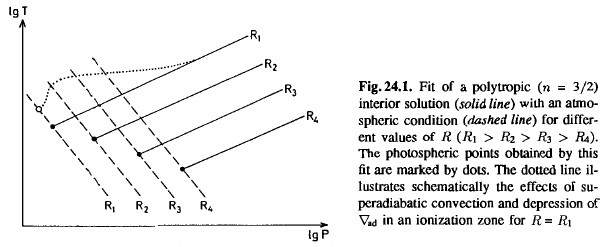
\includegraphics[trim={0cm 0cm 0 0},clip, keepaspectratio,width=0.90\textwidth]{HL-intatm}\label{fig:HL-intatm}
			\end{figure}
			\begin{figure}[!ht]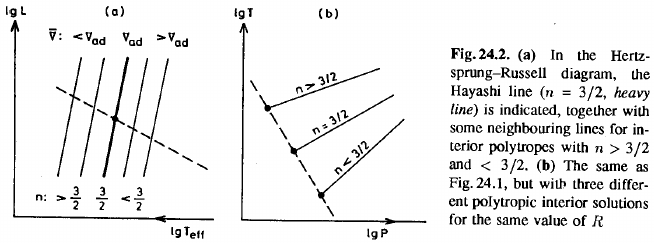
\includegraphics[trim={0cm 0cm 0 0},clip, keepaspectratio,width=0.90\textwidth]{HL-fulladiabatneigh}\label{fig:HL-fulladiabatneigh}
		\end{figure}
		\end{column}
	\end{columns}
\end{frame}

\begin{frame}{Burning of light elements in pre-MS (Hartmann97, Tognelli 2017)}
    \begin{columns}[T]
        \begin{column}{0.5\textwidth}
    Contrazione su $\tau\approx\tkh{}$ fino a innesco reazioni nucleari, in cui $L\propto t^{-\frac{2}{3}}$; nel caso si raggiungano le temperature di soglia per elementi leggeri si arresta contrazione ($\tau\approx\tau_n$).
            \begin{align*}
                &p(^2H,\APelectron\nu)^3He\tag{$T\approx\SI{e6}{\kelvin}$}\\
                &p(^6Li,^3He)^4He\tag{$T\approx\SI{2e6}{\kelvin}$}\\
                &p(^7Li,^4He)^4He\tag{$T\approx\SI{2.5e6}{\kelvin}$}\\
                &p(^9Be,^4He)^6Li\tag{$T\approx\SI{3.5e6}{\kelvin}$}\\
                &p(^{10}B,^4He)^7Be\tag{$T\approx\SI{4.5e6}{\kelvin}$}\\
                &p(^{11}B,2 ^4He)^4He\tag{$T\approx\SI{5e6}{\kelvin}$}
            \end{align*}
            $T_{Th}(X_i)>T_{bcz}$: Elemento $X_i$ non viene bruciato.
        \end{column}
        \begin{column}{0.5\textwidth}
			\begin{figure}[!ht]
                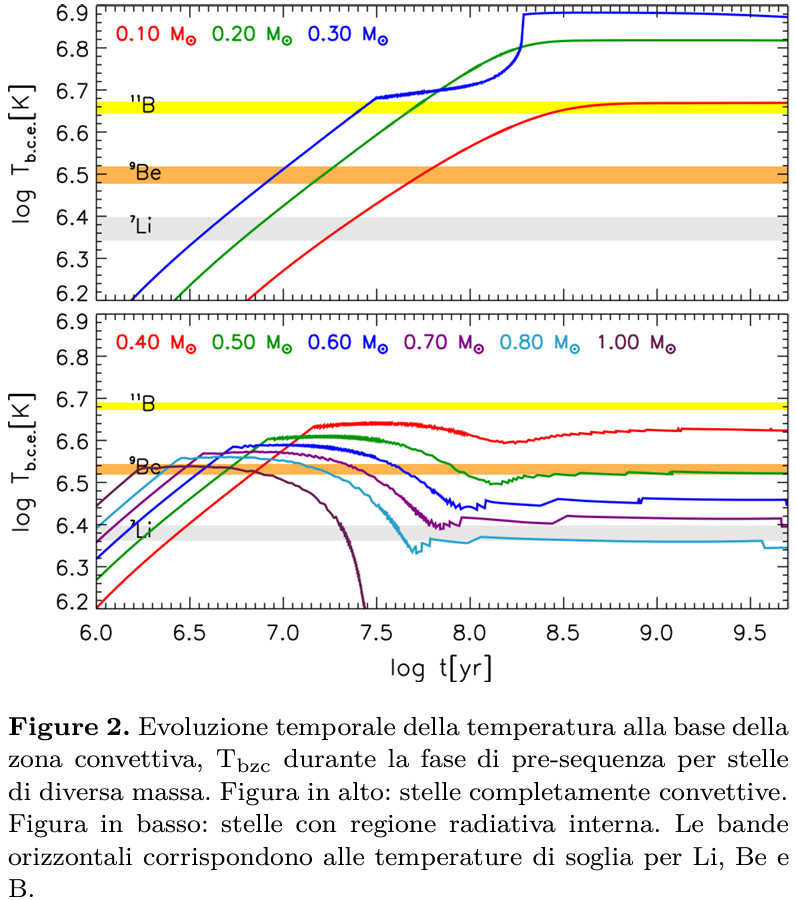
\includegraphics[trim={0cm 0cm 0 0},clip, keepaspectratio,height=0.45\textheight]{preMS-Tbcz}\label{fig:preMS-Tbcz}
			\end{figure}
        \end{column}
    \end{columns}
    
			\begin{figure}[!ht]
                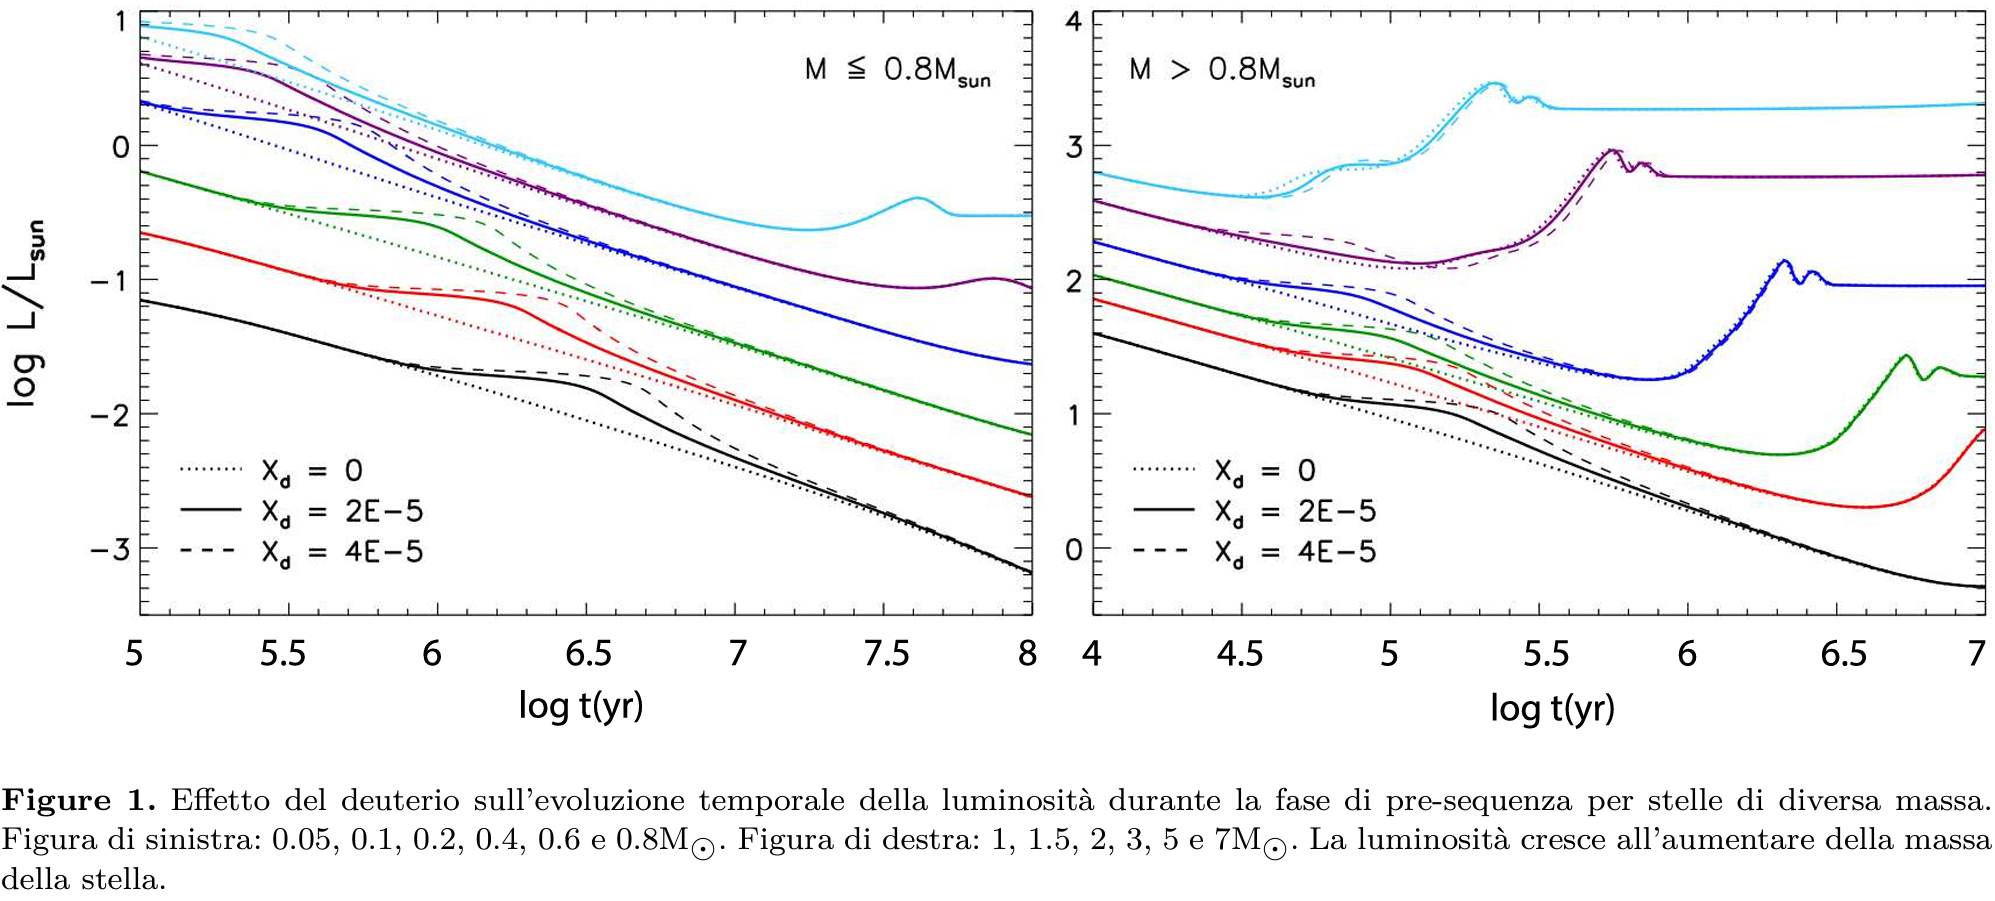
\includegraphics[trim={0cm 0cm 0 0},clip, keepaspectratio,height=0.45\textheight]{preMS-L}\label{fig:preMS-L}
			\end{figure}
\end{frame}

\subsection{Evoluzione di sequenza principale}\linkdest{MS}

\begin{frame}{Approccio alla ZAMS per stelle di sequenza superiori/inferiori}
dipendenza della ZAMS dall'abbondanza originale di He e metalli; metodo determinazione $DY/DZ$ dal confronto teoria-osservazione per stelle di disco locale parallassate; dipendenza massa minima di transizione dall'abbondanza di He e metalli; influenza sulla ZAMS dell'incertezza degli input fisici e dell'efficienza della convezione
\end{frame}

\begin{frame}{Yield of H-burning star analysis}
    \begin{columns}[T]
        \begin{column}{0.5\textwidth}
    \begin{itemize}
\item Longest evolutionary phase: larger number of observed stars
\item central/shell-H-burning determine successive phases
\item most important clock is central H-burning termination
\item Final shell H-burning phase in low mass, low-Z star provide distance indicator for old stellar pop
\item count of stars evolving through central H-burning give insight on IMF
\end{itemize}
        \end{column}
        \begin{column}{0.5\textwidth}
            \begin{figure}[!ht]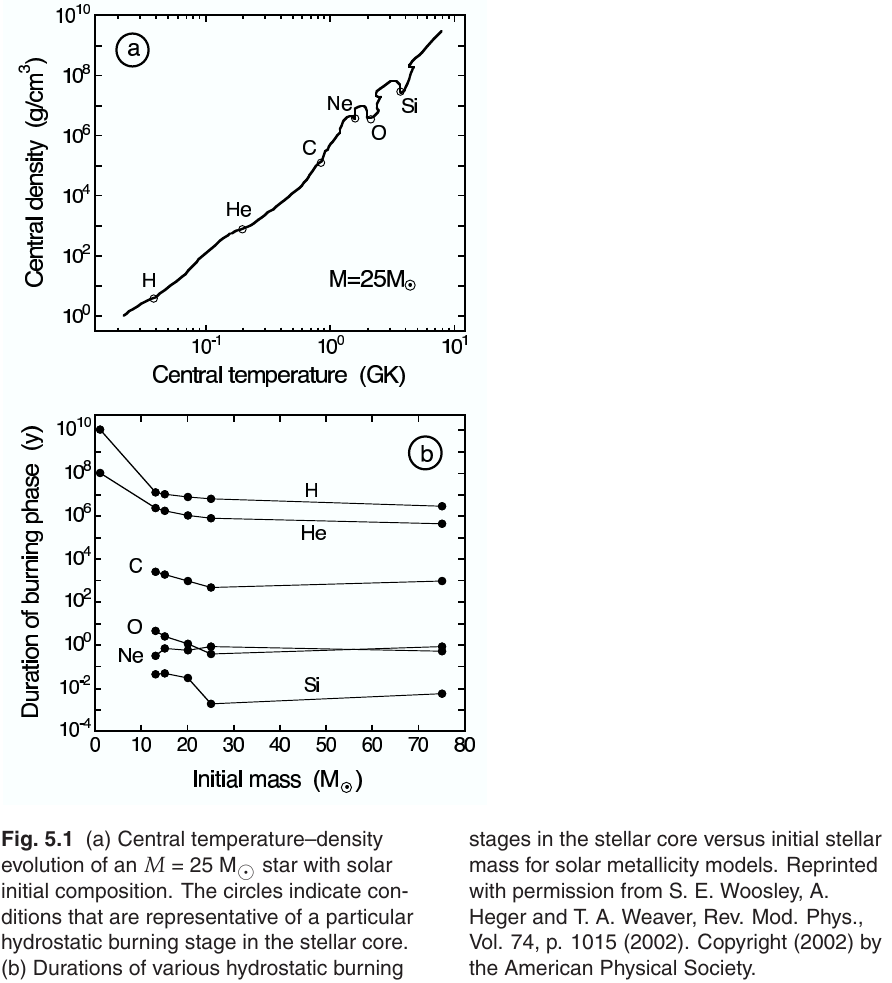
\includegraphics[trim={0.0cm 0cm 0.0cm 0},clip, keepaspectratio,width=0.95\textwidth]{burninglifetime}
			\end{figure}
        \end{column}
    \end{columns}
    
\end{frame}

\begin{frame}[fragile]{Major H burning reaction: PP chains}
\begin{columns}[T]\begin{column}{0.35\textwidth}
\begin{align*} 
&T\geq\SI{5e6}{\kelvin}\\
&^1H+^1H\to^2D+\APelectron+\Pnue\\
&^2D+^1H\to^3He+\gamma\\
&T\geq\SI{8e6}{\kelvin}:\\
&^3He+^3He\to^4He+2^1H\tag*{PPI}\\
&T\geq\SI{15e6}{\kelvin}:\\
&^3He+^4He\to^7Be+\gamma\\
&^7Be+\Pelectron\to^7Li+\Pnue\\
&^7Li+^1H\to^4He+^4He\tag*{PPII}\\
&^7Be+^1H\to^8B+\gamma\\
&^8B\to^8Be+\APelectron+\Pnue\\
&^8Be\to2^4He\tag*{PPIII}
\end{align*}
\end{column}\begin{column}{0.65\textwidth}
\begin{comment} 
\begin{align*}
&r_{pp}=\num{11.5e10}\rho^2X_H^2T_6\expy{-2/3}\\
&\exp{-33.81T_6\expy{-1/3}}(1+\num{0.0123}T_6\expy{1/3}+\num{0.0109}T_6\expy{2/3}\\
&+\num{0.00095}T_6)\\
&\rho\epsilon(3H\to^3He)=\\
&(\SI{6.936}{\mega\ev}-\SI{0.263}{\mega\ev})*\SI{1.602e-6}{\erg}*r_{pp}\\
&\rho\epsilon(^3He(^3He,2p)^4He)=\\
&(\SI{6.936}{\mega\ev}-\SI{0.263}{\mega\ev})*\SI{1.602e-6}{\erg}*r_{pp}\\
&\frac{PPI}{PPII+PPIII}=\frac{r_{33}}{r_{34}}=\frac{\lambda_{33}(^3He)^2/2}{\lambda_{34}^3He^4He}
\end{align*} 
\end{comment}
\begin{itemize}
    \item $Q=4*\massexcess{H}-\massexcess{^4He}=4*\SI{7288.97}{\kilo\ev}-\SI{2424.92}{\kilo\ev}=\SI{26.731}{\mega\ev}$ - energy release per gram $Q/m(^4He)=\SI{6.4e18}{\erg\per\gram}$ (Mass-excess: $\Delta m(A,Z)=M(A,Z)-A*u$)
    \item Energia nucleare: $n_p\approx \frac{\msun{}X}{m_p}\approx \frac{\num{2e33}*0.7}{\num{1.67e-24}}\approx\num{e57}$ protons, $E_{nucl}\approx \frac{\num{e57}\SI{26.1}{\mega\ev}}{4}\approx\SI{6e57}{\mega\ev}$
    \item Neutrino's Flux: $\Phi_{\nu}=\frac{n_{\nu}}{4\pi D^2}=\frac{2 \frac{\lsun{}}{\SI{26.1}{\mega\ev}}}{4\pi D^2}=\frac{\num{1.9e38}\nu/s}{\num{2.82e27}}\approx \frac{\num{6.7e10}\nu}{\si{\square\cm\second}}$, $\lsun{}\approx\SI{2.5e39}{\mega\ev\per\second}$, $D\approx\SI{1.5e13}{\cm}$.
\item Neutrino releases: PPI - \SI{0.5}{\mega\ev} per He
\item Neutrino releases: PPII - \SI{0.81}{\mega\ev} per He
\item Neutrino releases: PPIII - \SI{6.71}{\mega\ev} per He
\item $\epsilon_{PP}\propto X^2\rho T^4$
\end{itemize}
\end{column}\end{columns}
\end{frame}

\begin{frame}{H burning: CN-NO cycle}
\begin{columns}[T]\begin{column}{0.4\textwidth}
        Ciclo CN-NO: $T\geq\SI{1.5e7}{\kelvin}$
\begin{align*}
&^{12}C+^1H\to^{13}N+\gamma\\
&^{13}N\to^{13}C\APelectron+\Pnue\\
&^{13}C+^1H\to^{14}N+\gamma\\
&^{14}N+^1H\to^{15}O+\gamma\\
&^{15}O\to^{15}N+\APelectron+\Pnue\\
&^{15}N+^1H\to^{12}C+^4He\tag*{CN}\\
&T\geq\SI{20e6}{\kelvin}\tag*{Branching Ratio: \num{e-4}}\\
&^{15}N+^1H\to^{16}O+\gamma\\
&^{16}O+^1H\to^{17}F+\gamma\\
&^{17}F\to^{17}O+\APelectron+\Pnue\\
&^{17}O+^1H\to^{14}N+^4He\\
&^{17}O(p,\gamma)^{18}F\tag{$1\%$}\\
&^{18}F\to^{18}O\APelectron\Pnue\\
&^{18}O(p,\alpha)^{15}N\\
&^{18}O(p,\gamma)^{19}F\\
&^{19}F(p,\alpha)^{16}O\\
&^{19}F(p,\gamma)^{20}Ne
\end{align*} 
\end{column}\begin{column}{0.6\textwidth}
    Chemical changes: (CN) \xdiminuisce{C},\xaumenta{N}; (CNO) \xdiminuisce{C}, \xaumenta{N}, \xdiminuisce{O}.
    \begin{align*}
&\epsilon_{CN}(T_6)=\epsilon_{CN}(25)(\frac{T_6}{25})^{16.7}\\
&\epsilon_{CNO}\propto XX_{14}\rho T^{18}\\
&
\end{align*}
Matter processed by CN: \xdiminuisce{C}, \xaumenta{N}; by CNO: \xdiminuisce{C}, \xaumenta{N}, \xdiminuisce{O}.
\end{column}\end{columns}
\end{frame} 

\subsection{Lower main sequence ($M^*\leq1.3\msun{}$)}\linkdest{LMS}

\begin{frame}{Da ZAMS a TO for $M^*\leq1.3\msun{}$}
    ZAMS: first MS model fully supported by H-burning in which secondary elements are in equilibrium (2 $^3He$ are consumed in $^3He+^3He$ reaction):
\begin{itemize}
\item $^3He$ production in central zones: si forma piccolo core convettivo
    \[\TDy{t}{N_{^3He}}=N_{^1H}N_D\exv{\sigma v}_{^1HD}-2\frac{(N_{^3He})^2}{2}\exv{\sigma v}_{^3He^3He}-N_{^3He}N_{^4He}\exv{\sigma v}_{^3He^4He}\]
    \begin{columns}[T]
        \begin{column}{0.5\textwidth}
            Assuming $N_{^3He}\gg N_{^3He}^{eq}$ we can estimate time scale for $^3He$ equilibrium: destruction is dominant; equations valid for radiative regions- in convective zone we take average.
        \end{column}
        \begin{column}{0.5\textwidth}
            \begin{align*}
                &\TDy{t}{N_3}\approx-2 \frac{(N_3)^2}{2}\exv{\sigma v}_{33}-N_3N_4\exv{\sigma v}_{34}\\
                &\tau_3=\frac{1}{N_3\exv{\sigma v}_{33}+N_4\exv{\sigma v}_{34}}
            \end{align*}
        \end{column}
    \end{columns}
    

\end{itemize}
\begin{columns}[T]\begin{column}{0.5\textwidth}
\begin{figure}[!ht]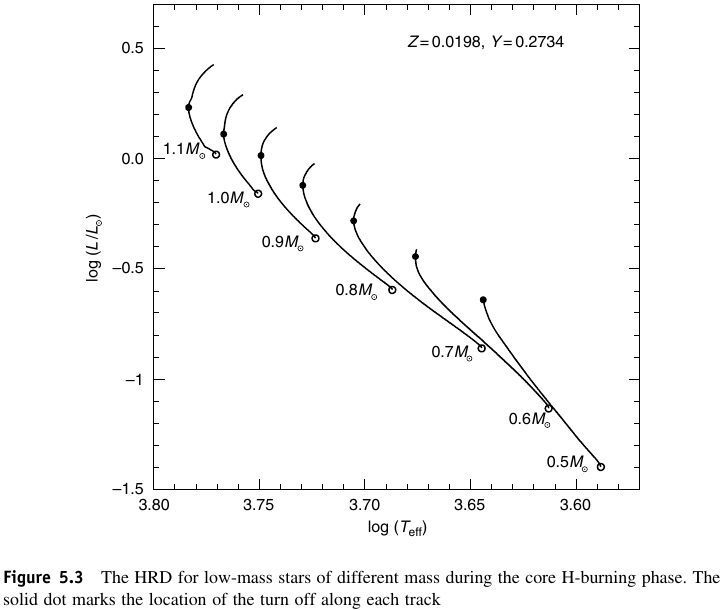
\includegraphics[trim={0cm 0cm 0 0},clip, keepaspectratio,width=0.99\textwidth]{HRD-LMS}\label{fig:HRD-LMS}
\end{figure}
\end{column}\begin{column}{0.50\textwidth}
    \begin{itemize}
        \item La stella continua a contrarsi fino alla partenza della reazione $^3He(^3He,2^1H)^4He$ e il core convettivo svanisce con l'espandersi della regione in cui \'e prodotto $^3He$
        \item Struttura: H-burn in central radiative core (Small T-dep of $\epsilon_{PP}$), convective envelope (large opacity associated to partial ionized H, He)
        \item Evoluzione: $\#$ free particles $\downarrow$, \xaumenta{\mu} per HE \xaumenta{T}, \xdiminuisce{R} quindi $L^*$ aumenta lentamente.
        \item TO is hottest point in evolutionary track: H exhausted 
\end{itemize}
\end{column}\end{columns}
\end{frame}


\subsection{Upper main sequence ($M^*\geq1.2-1.3\msun{}$)}\linkdest{UMS}

\begin{frame}{Da ZAMS a Overall contraction}
\begin{columns}[T]\begin{column}{0.5\textwidth}
\begin{figure}[!ht]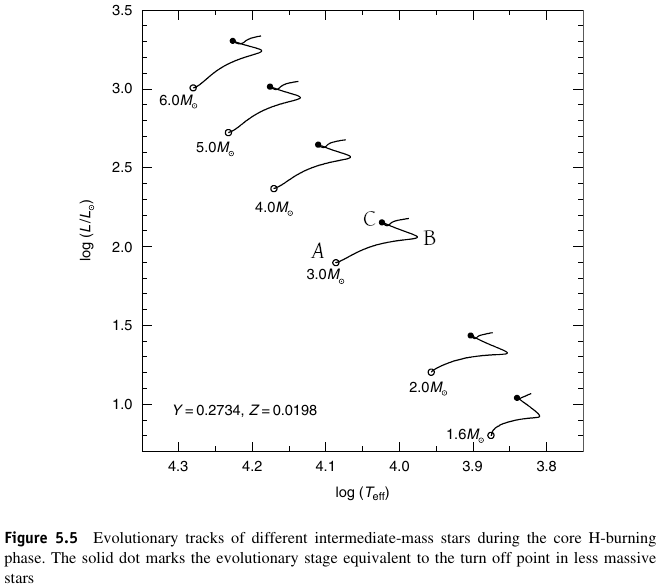
\includegraphics[trim={0cm 0cm 0 0},clip, keepaspectratio,width=0.7\textwidth]{HRD-UMS}\label{fig:HRD-UMS}
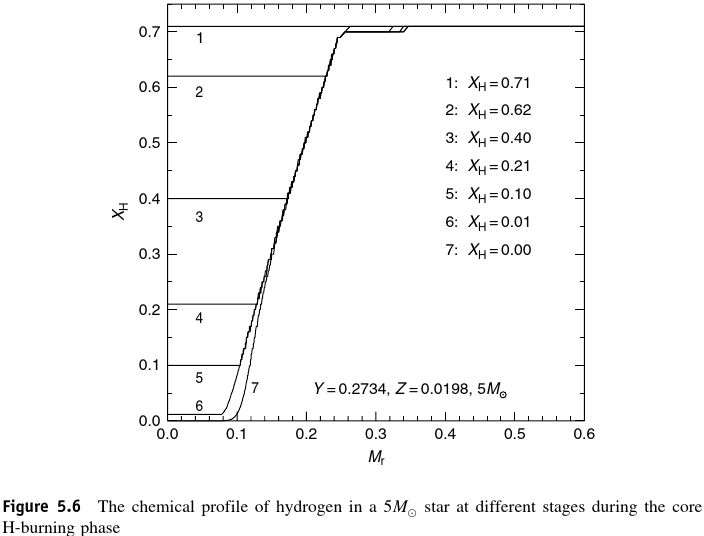
\includegraphics[trim={0cm 0cm 0 0},clip, keepaspectratio,height=0.40\textheight]{UMS-Hprofile}\label{fig:UMS-Hprofile}\end{figure}
\end{column}\begin{column}{0.5\textwidth}
\begin{block}{CNO H-Burning: convective core}
Higher T: CNO dominant: $\epsilon_{CNO}$ steeper:convective core: \xaumenta{M^*}, \xaumenta{M_{con}}, \xaumenta{P_{rad}}, \xdiminuisce{\nad{}}.
\end{block}
\begin{block}{As UMS burn H}
\begin{itemize}
    \item convective core shrink: ?\xaumenta{\mu}, \xaumenta{P_c}?
    \item radius expands: after H exhaustion
    \item core gravitationally contract
    \item $L$ increases such that $T_e$ has little drop
\end{itemize}
\end{block}
\begin{block}{Overall contraction}
    When $X<0.05$ at B start gravitational contraction of core until C; after C inner regions contract outer expand; C mark ends of central H-burning phase: after C core contracts and outer envelope expands and thus radius increases and outer opacity increases while T outer layers decreases.
\end{block}
\begin{block}{Core retraction leaves He gradient}
    Convective core retracts as X is strongly decreased leaving He gradient decreasing moving outwards.
\end{block}
\end{column}\end{columns}
\end{frame}

\begin{frame}{Details of $5\msun{}$}
    \begin{columns}[T]
        \begin{column}{0.6\textwidth}
\begin{figure}[!ht]
    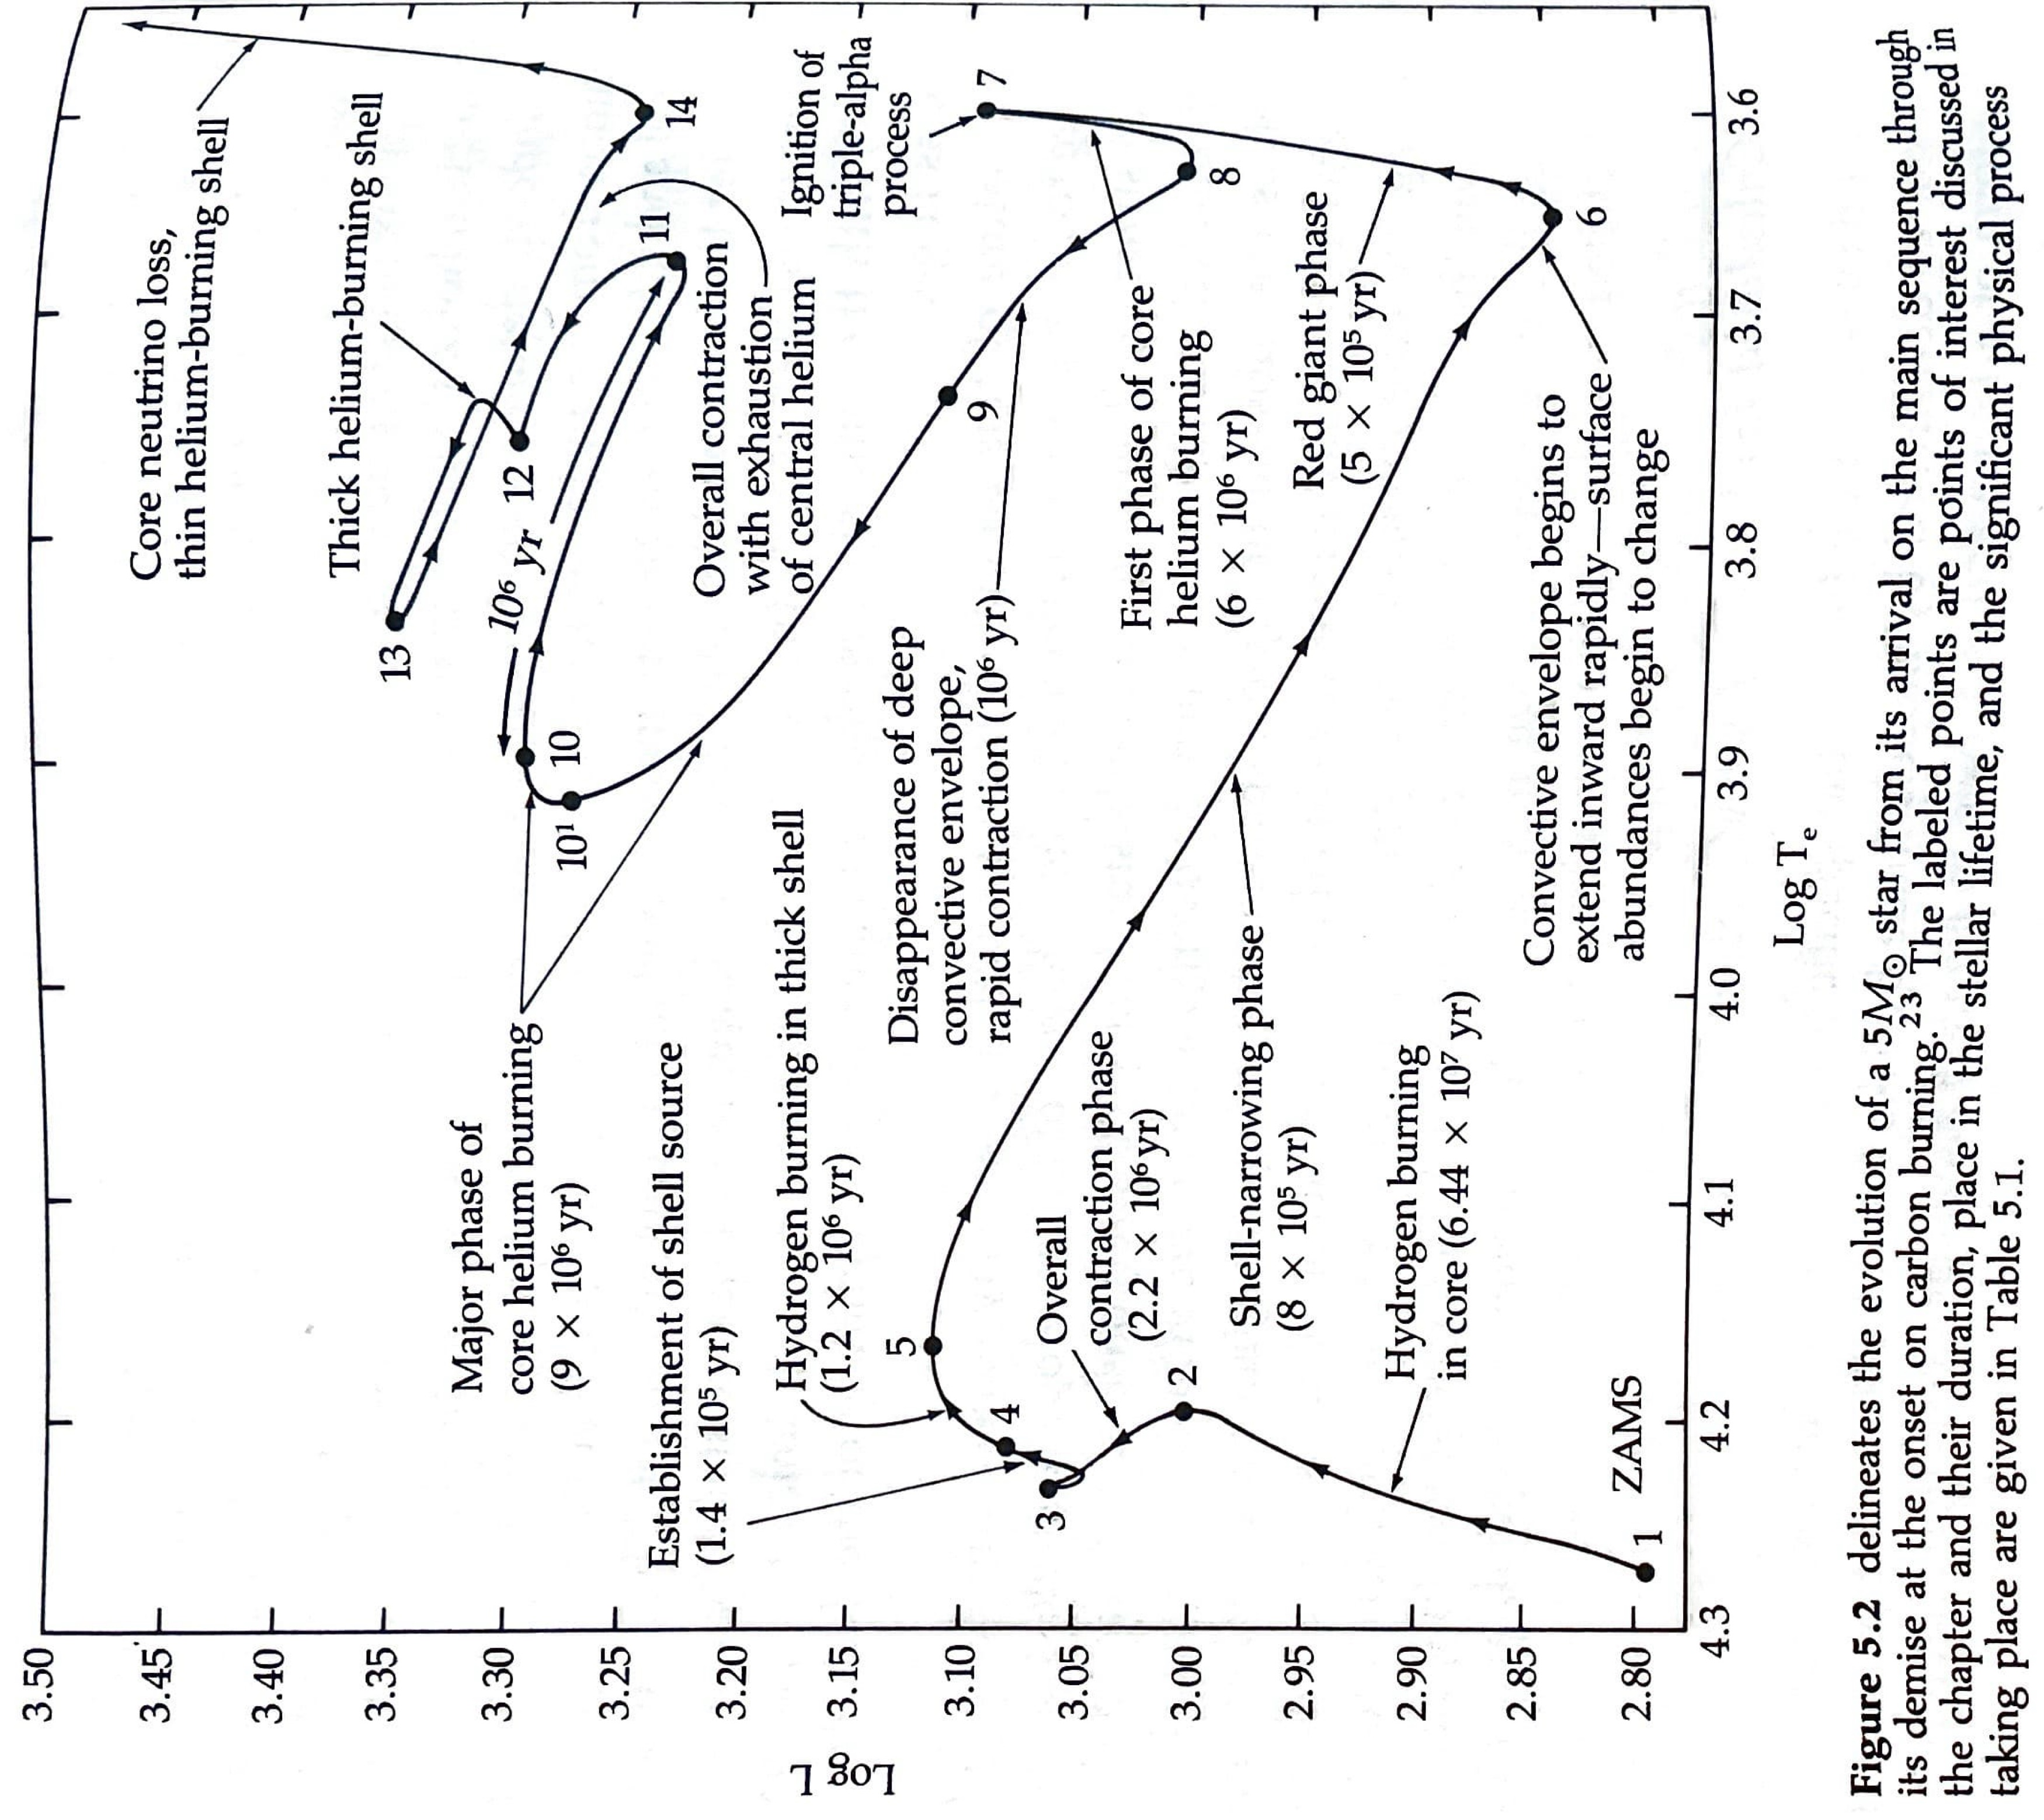
\includegraphics[trim={0cm 0cm 0 0},clip, keepaspectratio,height=0.8\textheight,origin=c,angle=-90]{5msun_detail}\label{fig:5msun_detail}
\end{figure}
        \end{column}
        \begin{column}{0.4\textwidth}
\begin{figure}[!ht]
    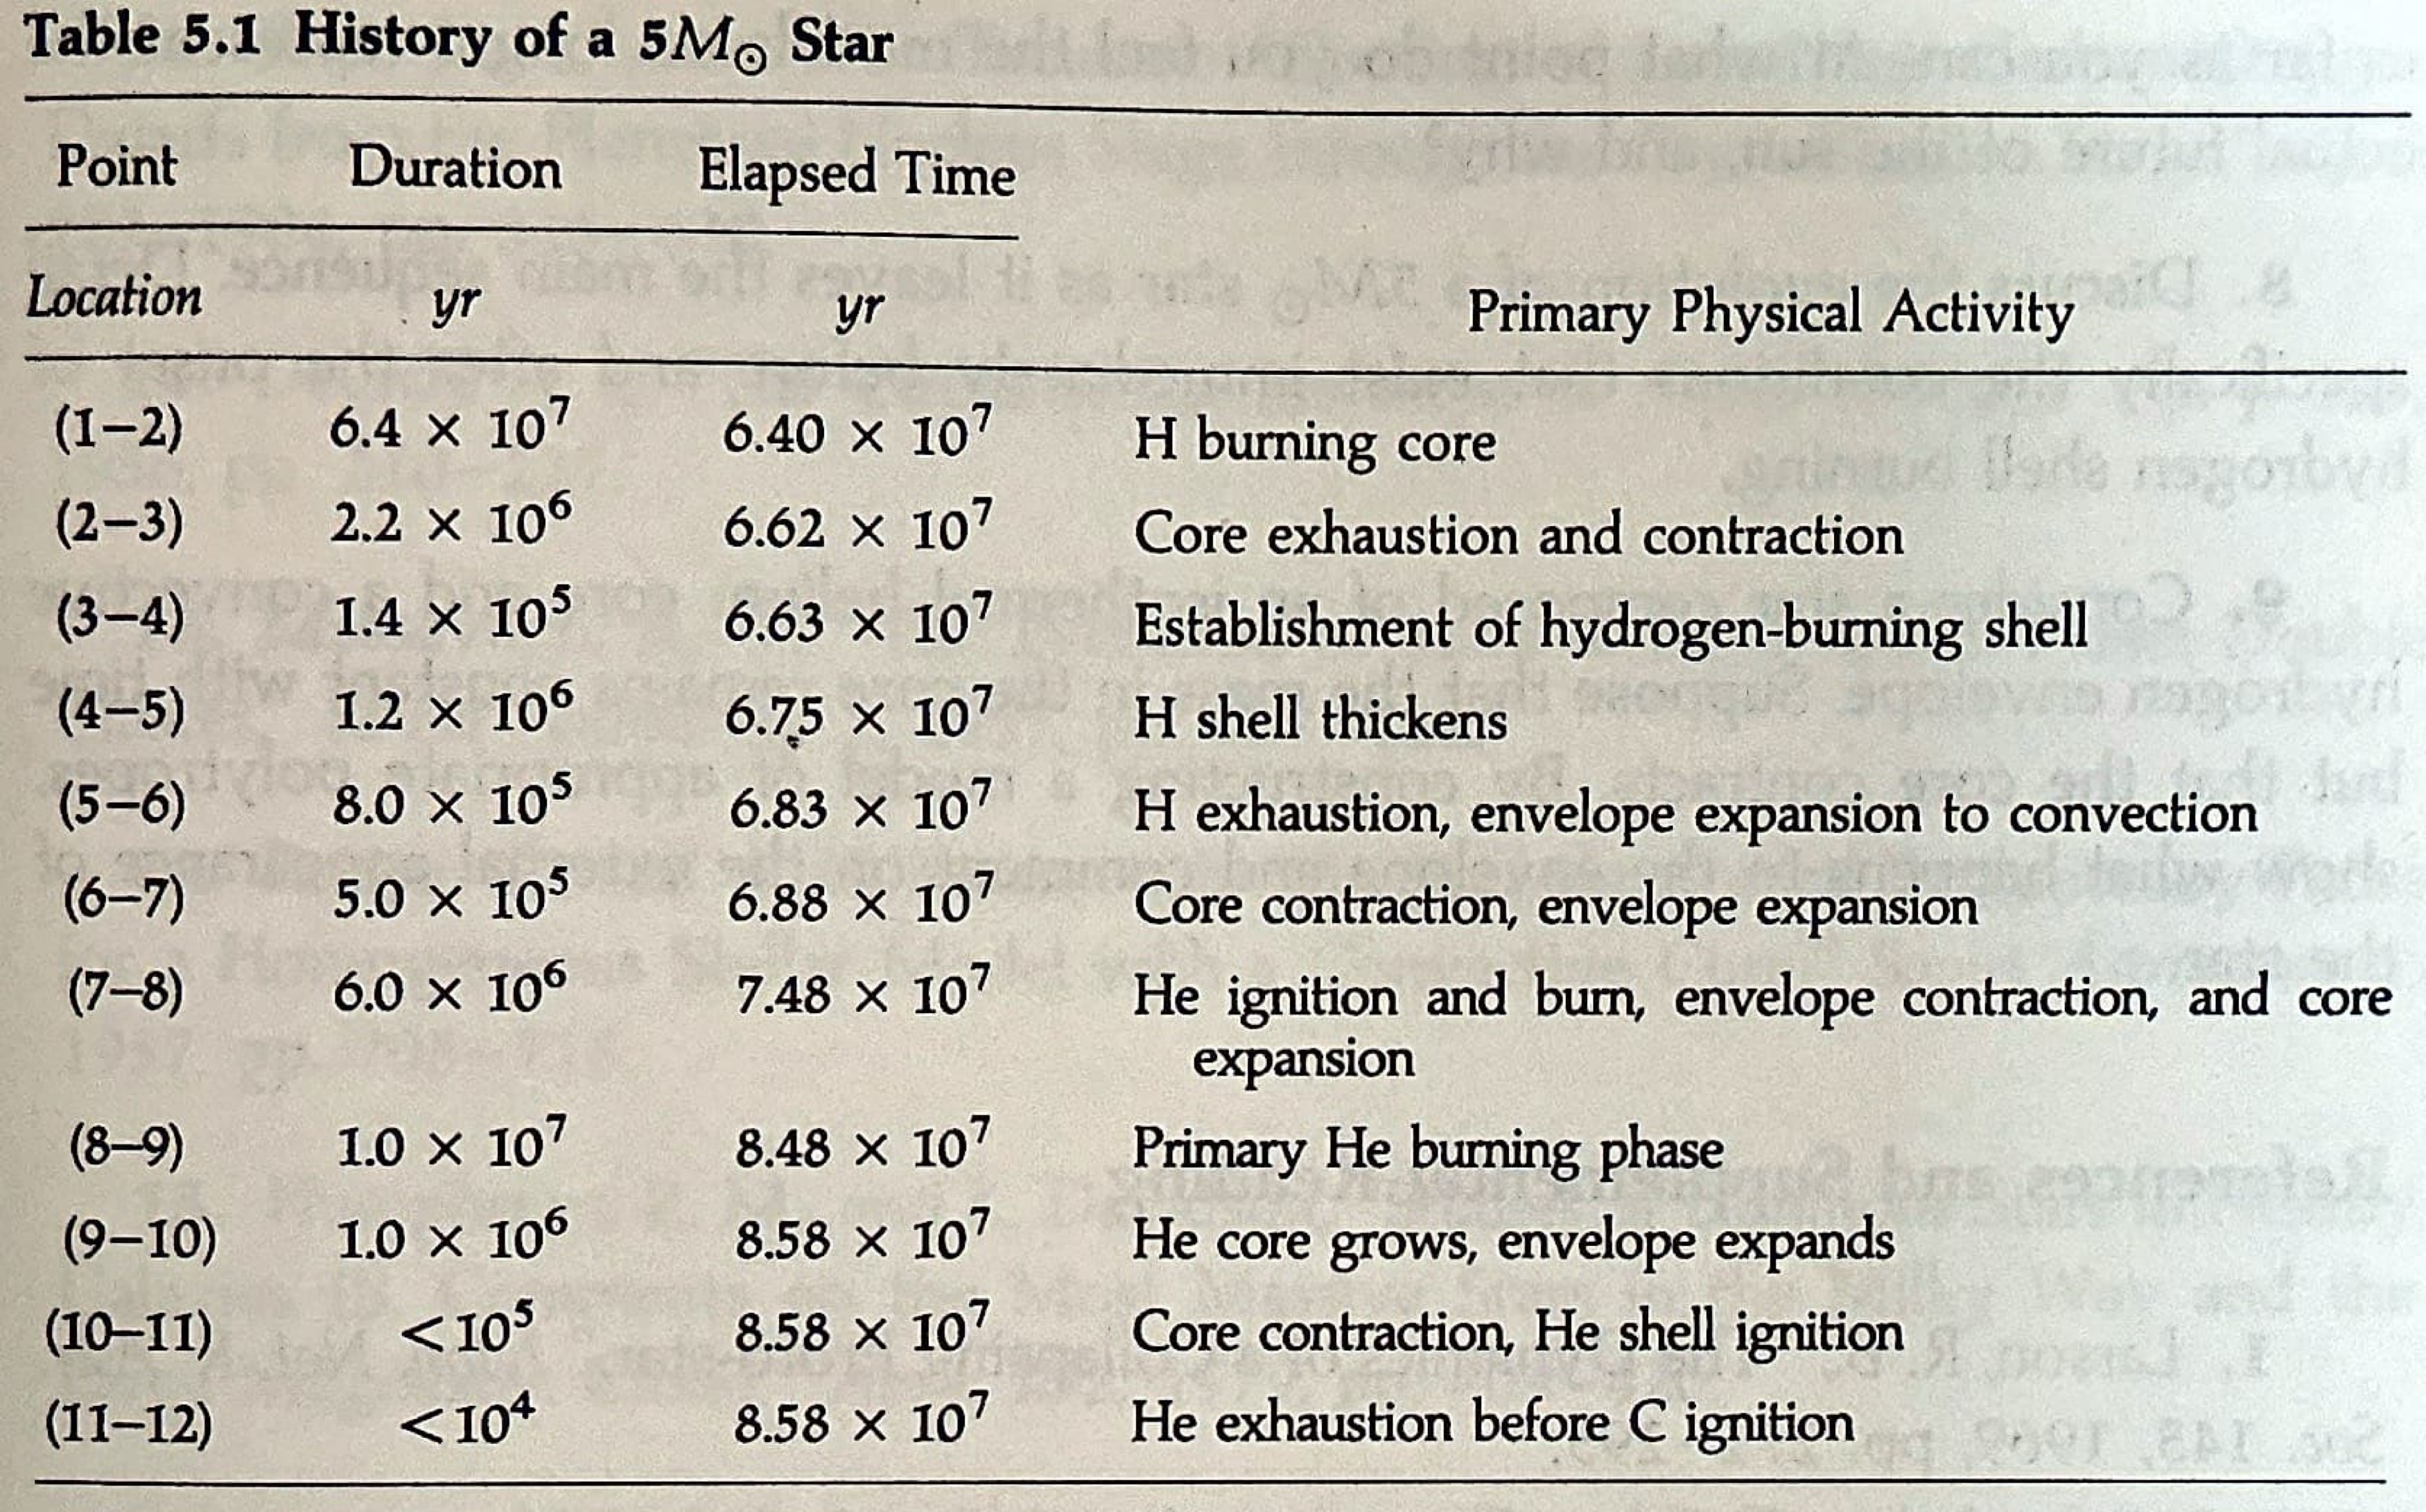
\includegraphics[trim={0cm 0cm 0 0},clip, keepaspectratio,width=0.95\textwidth,origin=c,angle=0]{5msun_tab}\label{fig:5msun_tab}
\end{figure}
        \end{column}
    \end{columns}
    
\end{frame}

\subsection{Deps of MS on Physical input}\linkdest{MSdeps}

\begin{frame}{Effects of changes in initial chemical composition}
\begin{block}{Different initial Y value: opacity and mean molecular weight}
\begin{columns}[T]
\begin{column}{0.5\textwidth}
\begin{figure}[!ht]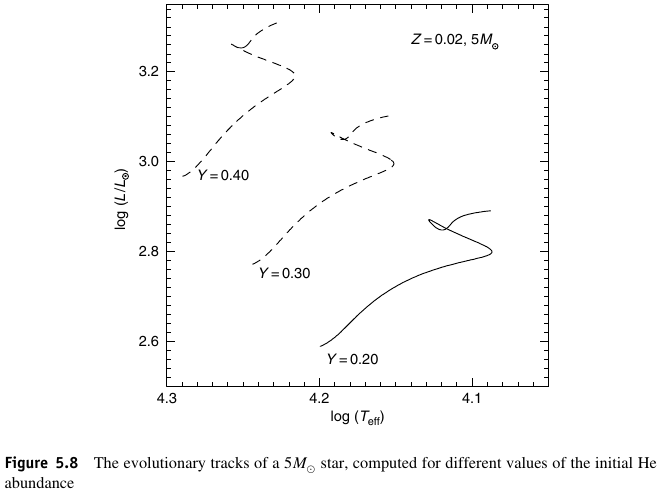
\includegraphics[trim={0cm 0cm 0 0},clip, keepaspectratio,width=0.99\textwidth]{HRD-changingHe}\label{fig:HRD-changingHe}
\end{figure}
\end{column}
\begin{column}{0.5\textwidth}
\begin{itemize}
    \item Increases of nuclear rates $L_H\propto\mu^7$
    \item Opacity decreases
\end{itemize}
Star is brighter and hotter
\end{column}
\end{columns}
\end{block}
\begin{block}{Changes in Z affect opacity}
\begin{itemize}
    \item \xaumenta{Z}, \xaumenta{\kappa}: fainter, cooler star.
    \item PP chain reaction not dependent on Z, CNO element are enough exept in pop III.
    \item $\alpha$-enhanced objects: CNO cycle efficiency increased, opacity increased with two bump at $\log{T}=6,5.5$ due to K shell O electrons and L-edges of Mg, Si, Ne. Stars are fainter and cooler
\end{itemize}
\end{block}
\end{frame}

\begin{frame}{Effects of changing convection efficiency: superadiabatic convection}
\begin{columns}[T]
\begin{column}{0.5\textwidth}
\begin{figure}[!ht]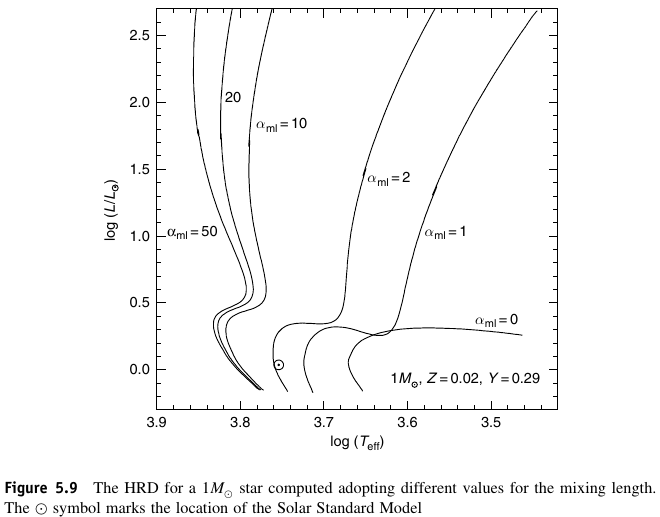
\includegraphics[trim={0cm 0cm 0 0},clip, keepaspectratio,width=0.99\textwidth]{HRD-1M-changingalpha}\label{fig:HRD-changingHe}
\end{figure}
\end{column}
\begin{column}{0.5\textwidth}
\begin{itemize}
    \item $\alpha_{ML}$ calibrated using Sun.
    \item $\alpha_{ML}$ does not affect L
    \item $\alpha_{ML}$ affects radius and $T_e$: \xaumenta{\alpha},\xdiminuisce{\nabla},\xaumenta{T_e},\xdiminuisce{R_s}
\end{itemize}
\end{column}
\end{columns}
\end{frame}

\begin{frame}{Convective core and Overshooting ($M>10\msun{}$)}
\begin{columns}[T]\begin{column}{0.5\textwidth}
\begin{figure}[!ht]
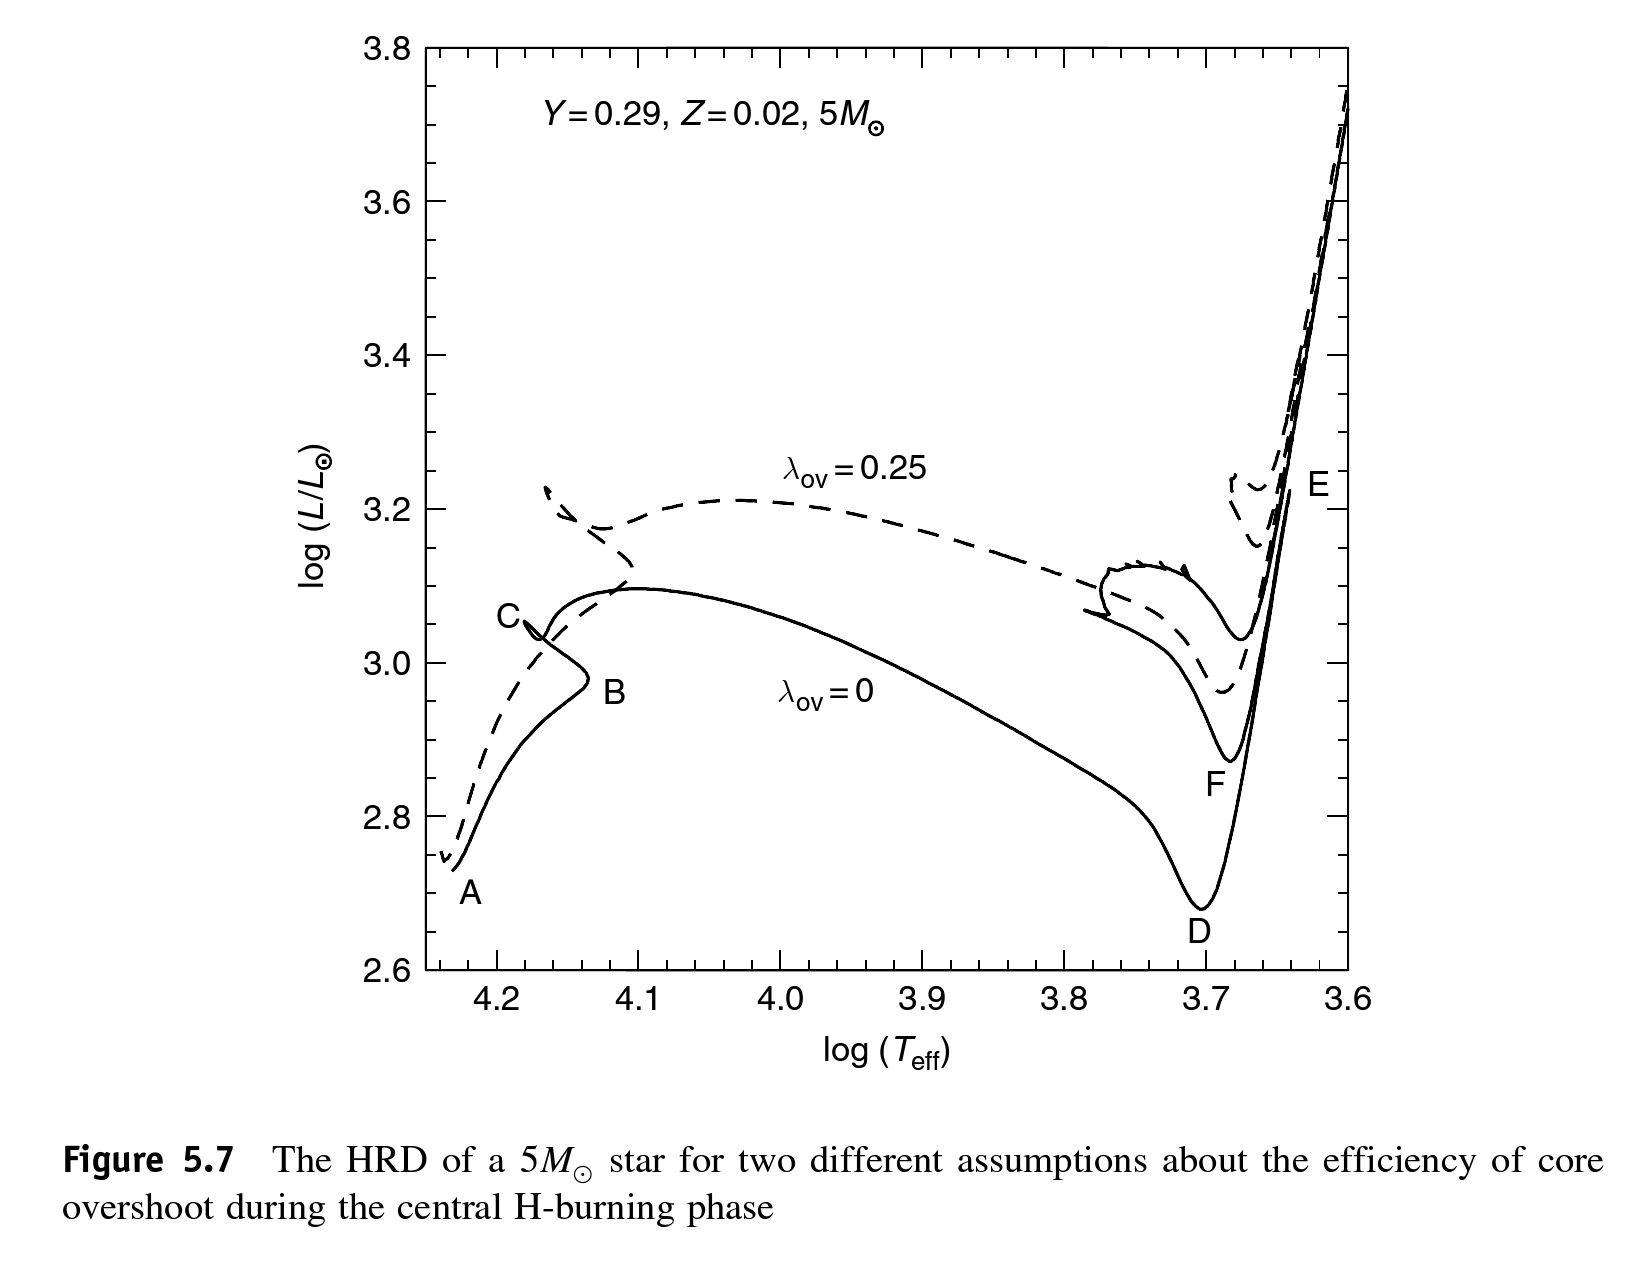
\includegraphics[trim={0cm 0cm 0 0},clip, keepaspectratio,height=0.42\textheight]{HRD-overshoot}\label{fig:HRD-overshoot}
\end{figure}
\end{column}
\begin{column}{0.5\textwidth}
\begin{block}{What increases convective core}
\begin{itemize}
\item Changes in physical input
\item Stellar rotation
\item Physical overshooting
\end{itemize}
\end{block}
\end{column}\end{columns}
\begin{columns}[T]\begin{column}{0.55\textwidth}
\begin{block}{Effects of increased convective core}
\begin{itemize}
\item \xaumenta{M_c}, \xaumenta{\mu} (involve more mass), \xaumenta{L}
\item Longer central H-burning
\item Larger He core at end of MS: brighter He-burning phase star, shorted lifetime
\end{itemize}
\end{block}
\end{column}
\begin{column}{0.45\textwidth}
\begin{block}{\sch vs Ledoux in-stability criterion}
In radiative region the retracting convective core leave chem composition gradient; but \xaumenta{He}, \xdiminuisce{\kappa}
\end{block}
\end{column}\end{columns}
\end{frame}

\begin{frame}{Low-mass star $M<0.4\msun{}$}
\begin{columns}[T]\begin{column}{0.45\textwidth}
\begin{figure}[!ht]
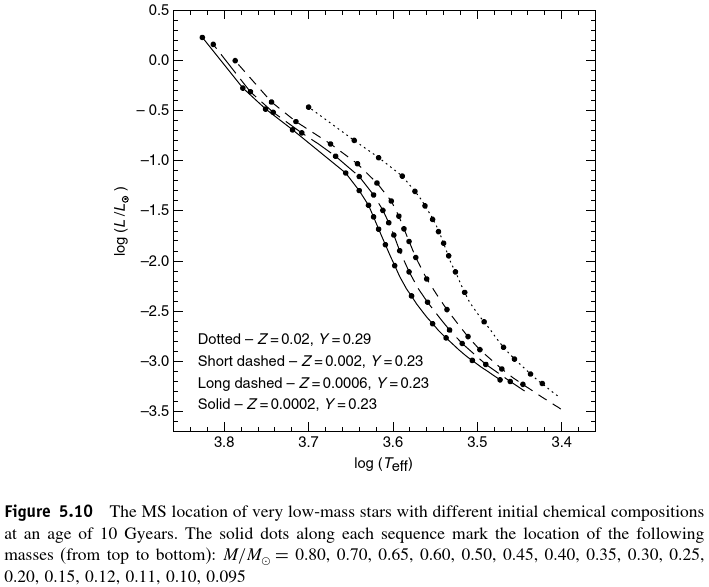
\includegraphics[trim={0cm 0cm 0 0},clip, keepaspectratio,width=0.99\textwidth]{VLM-HDR}\label{fig:VLM-HDR}
\end{figure}
\end{column}
\begin{column}{0.47\textwidth}
\begin{itemize}
    \item Fully convective through MS live
    \item PP1 H-burning with negligible $^3He$ destruction
    \item Transition between molecular H and atomic He to plasma at inner $90\%$ in mass: thermodynamical properties sensible to treatment of pressure ionizzation, dissociation, non-ideal Coulomb.
    \item Atmospheric features due to opacity sources: collisional induced dipole in $H_2$ molecules, CIA suppresses flux at \SI{2}{\micro\meter}; for $T_e<\SI{4000}{\kelvin}$ molecules of $TiO$ and $VO$ controll flux in optical, $H_2O$ and $CO$ the flux in infrared; for $T_e<\SI{2800}{\kelvin}$ also grains are important.
\end{itemize}
\end{column}\end{columns}
\end{frame}

\subsection{Mass-Luminosity relations: $L\propto M^3$}\linkdest{malure}

\begin{frame}{M-L relation}
\begin{columns}[T]\begin{column}{0.4\textwidth}
Near ZAMS $L\propto M^3$:
\begin{align*}
    &T^3\TDy{m_r}{T}=-\frac{3\kappa_R}{64\pi^2ac}\frac{L_r}{r^4}\Rightarrow L\propto \frac{R^4}{M}T_c^4\\
    &\TDy{m_r}{P}=-\frac{Gm_r}{4\pi r^4}\Rightarrow P\propto \frac{M^2}{R^4}\\
    &P\propto\rho T\propto \frac{M}{R^3}T\Rightarrow T_c\propto \frac{M}{R}
\end{align*}
\begin{figure}[!ht]
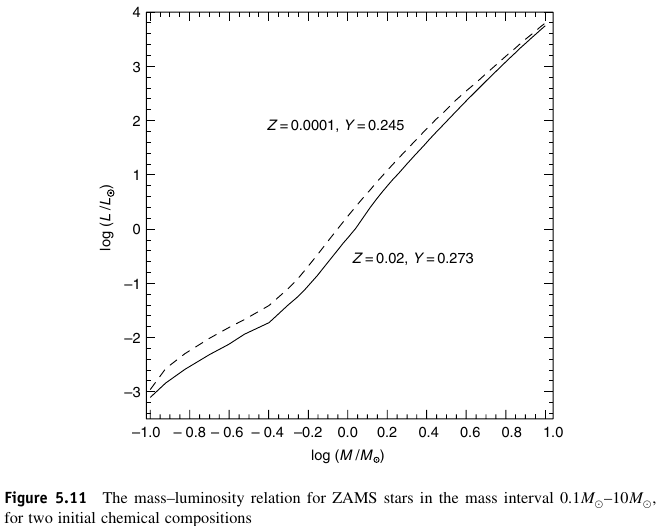
\includegraphics[trim={0cm 0cm 0 0},clip, keepaspectratio,width=0.99\textwidth]{ML-01-10}\label{fig:ML-01-10}
\end{figure}
\end{column}
\begin{column}{0.6\textwidth}
Scilla's Version:
\begin{align*}
    &\exv{\rho}\propto \frac{M}{R^3},\TDy{r}{P}=-\frac{\rho GM}{r^2}\Rightarrow \frac{P_e-P_c}{R-0}\propto-\frac{GM}{R^2}\frac{M}{R^3}\\
    &\Rightarrow P_c\propto\frac{M^2}{R^4},\ P\approx P_g=\frac{\rho}{\mu m_u}KT:\\
    &T_c\propto \frac{P_c\mu_c}{\rho_c}\propto \frac{P_c\exv{\mu}}{\exv{\rho}}\propto\frac{M^2}{R^4}\frac{R^3}{M}\exv{\mu}\Rightarrow T_c\propto \frac{M}{R}\exv{\mu}\\
    &\TDy{r}{T}|_{Rad}=-\frac{3}{4\pi ac}\frac{\exv{\kappa}\rho}{T^3}\frac{L(r)}{4\pi r^2}: L\propto-\frac{T^3}{\exv{\kappa}\rho}\TDy{r}{T}r^2\\
    &\Rightarrow L\propto \underbrace{\frac{M}{R^2}\mu}_{\TDy{r}{T}}\underbrace{\frac{M^3}{R^3}\exv{\mu}^3}_{T^3}\frac{1}{\exv{\kappa}}\underbrace{\frac{R^3}{M}}_{\frac{1}{\exv{\rho}}}R^2\propto \frac{\exv{\mu}^4M^3}{\exv{\kappa}}\tag{M-L relation}\\
    &\TDy{r}{L}=4\pi r^2\exv{\rho}\epsilon: \frac{L}{R^3}\propto\exv{\rho}\epsilon\Rightarrow\exv{\rho}\propto \frac{L}{R^3}\frac{1}{\epsilon}\\
    &T_c\propto \frac{M}{R}\Rightarrow R\propto \frac{M}{T}: \exv{\rho}\propto \frac{L}{M^3}\frac{T^3}{\epsilon}, L\propto M^3: \exv{\rho}\propto \frac{T^3}{\epsilon}\\
    &\epsilon\propto\rho^mT^n\tag{H fusion: $m=1$, PP: $n\approx4$, CN-NO: $n\approx\numrange{15}{17}$}\\
    &\Rightarrow\rho\propto \frac{T^3}{\rho^mT^n}: \rho^{m+1}\propto T^{3-n}\Rightarrow\rho^2\propto T^{3-n}
\end{align*}
    Relazione osservativa
\begin{equation*}
L\propto\begin{array}{l}
M\expy{3.6},\ \numrange{2}{20}\msun{}\\
M\expy{4.5},\ \numrange{0.5}{2}\msun{}\\
M\expy{2.6},\ \numrange{0.2}{0.5}\msun{}\\
\end{array}
\end{equation*}
For $M,\ M>10\msun{}$ relation becomes less steep $L\propto M$: due to increasing contribution of radiation pressure in massive stars.
\end{column}\end{columns}
\end{frame}

\subsection{Post-MS: SGB(const L, move Blue to Red), RGB (const T, L increases)}\linkdest{postMS}
%SC [160]

%\begin{frame}{Int-massive stars}
%\begin{figure}[!ht]
%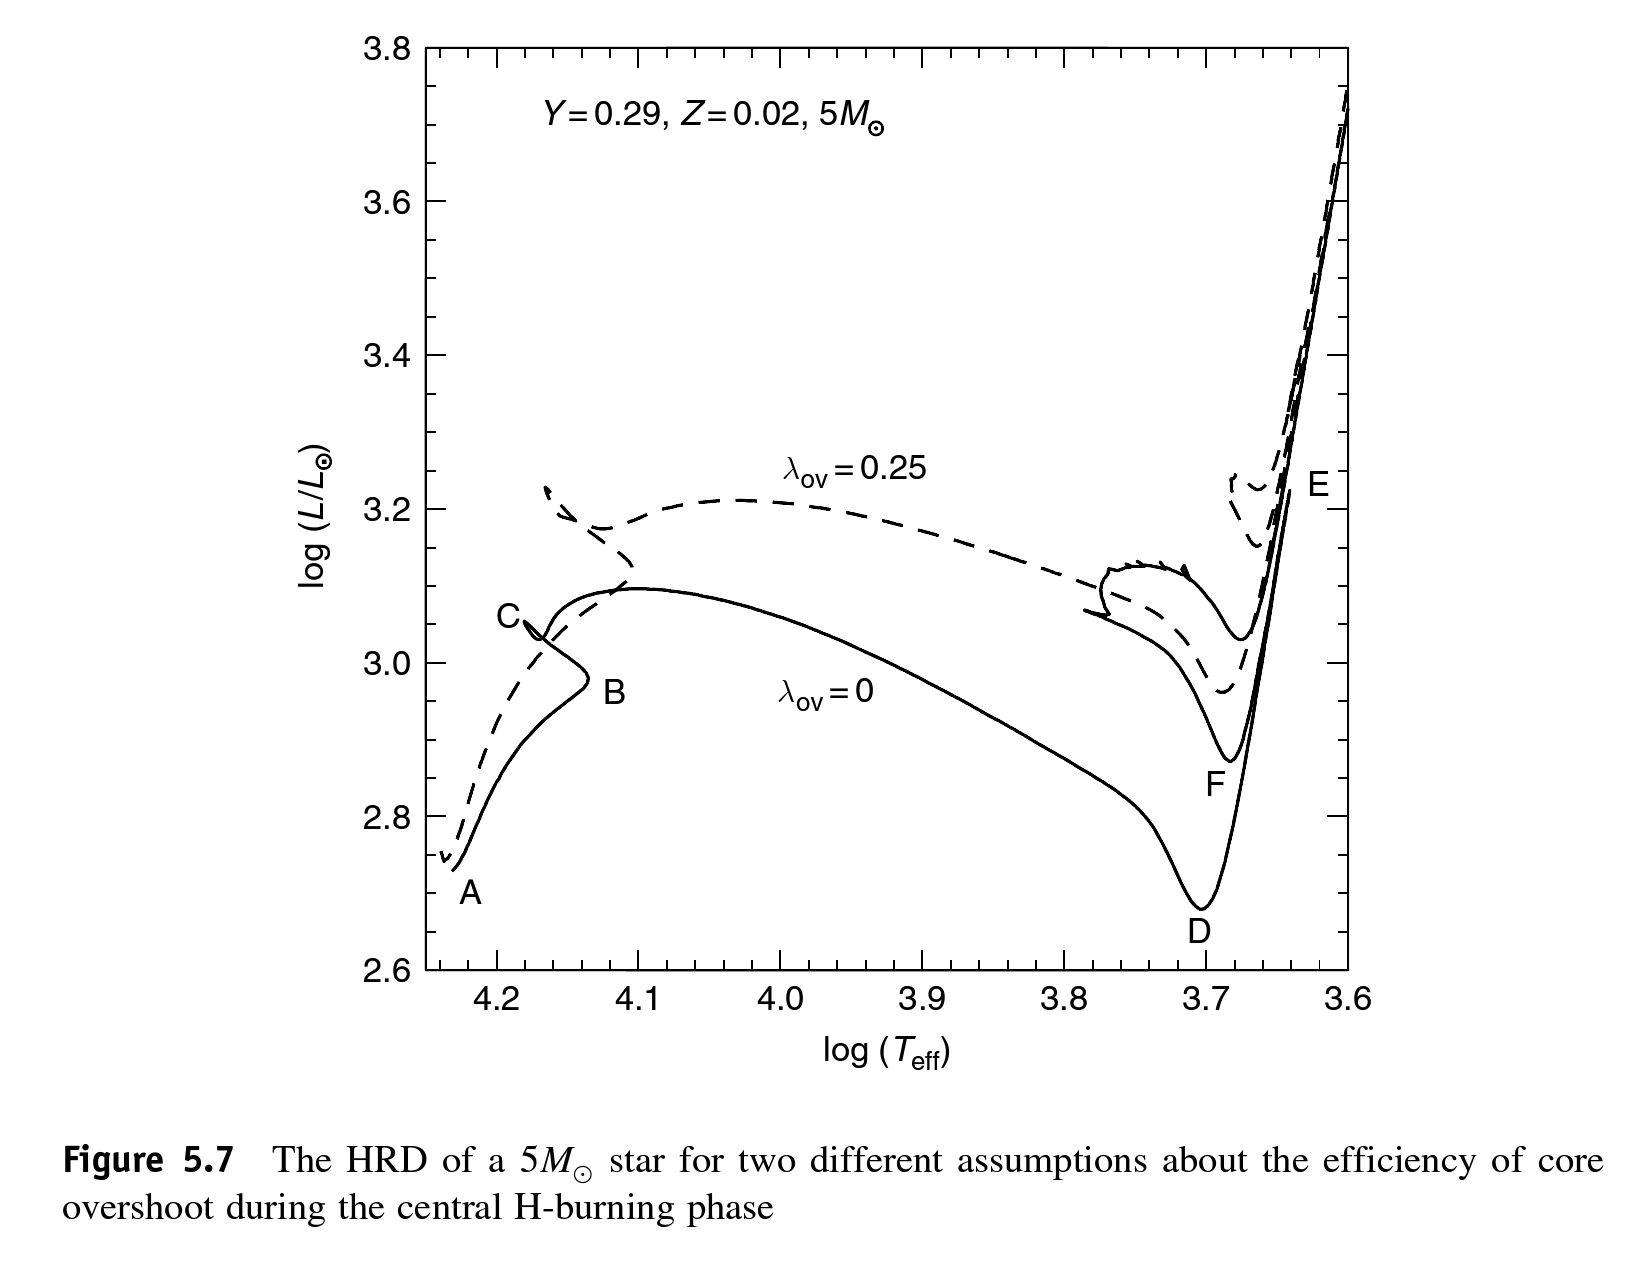
\includegraphics[trim={0cm 0cm 0 0},clip, keepaspectratio,height=0.42\textheight]{HRD-overshoot}\label{fig:HRD-overshoot}
%\end{figure}
%    \begin{itemize}
%        \item $M_{He,core}$ maggiore del limite SC
%        \item SGB: Structure move from blue to red side at almost constant surface L. $\tkh{}\approx\SI{12}{\mega\year}$ for $3\msun{}$, $\tkh{}\approx\SI{1}{\mega\year}$ for $6\msun{}$.
%        \item RGB: Point D - constant effective T while L increases; point E where He burning is efficient marks the end of RG phase.
%    \end{itemize}
%\end{frame}

\begin{frame}{Condizione Core per fusione: Virial theorem}
    \begin{columns}[T]
        \begin{column}{0.65\textwidth}
\begin{itemize}
    \item gravitational contraction: virial theorem
        \begin{align*}
            &\int_0^M\TDy{m}{P}4\pi r^3\,dm=-\int_0^M \frac{Gm}{r}\,dm\tag{HE$*4\pi r^3$}\\
            &\Rightarrow \underbrace{[4\pi r^3P]_0^M}_{P_{surf}\approx0,r=0}-\int_0^M12\pi r^2\TDy{m}{r}P\,dm=-\int_0^M \frac{Gm}{r}\,dm\\
            &E=\frac{3}{2}\frac{P}{\rho}\Rightarrow E=-\frac{\Omega}{2}\tag{Internal energy per unit mass: perfect monoatomic gas}\\
            &E_T=E+\Omega\Rightarrow E_T=-E, E_T=\frac{\Omega}{2}\\
            &L=-\TDy{t}{E_T}\Rightarrow L=-\frac{1}{2}\TDy{t}{\Omega}, \Delta E=-\Delta E_T=\frac{\Delta\Omega}{2}\tag{only grav}\\
            &E=\frac{1}{\gamma-1}\frac{P}{\rho}, \gamma=\frac{c_P}{c_v}(=\frac{5}{3}\text{perfect})\tag{generic perf. gas}\\
            &\Rightarrow E=-\frac{\Omega}{3(\gamma-1)},E_T=\frac{3\gamma-4}{3(\gamma-1)}\Omega\tag{Stability: HE $\gamma>\frac{4}{3}$}\\
            &3(\gamma-1)E+\Omega=4\pi R^3P_0\tag{Surf. press.}\\
        \end{align*}
\end{itemize}
        \end{column}
        \begin{column}{0.35\textwidth}
\begin{figure}[!ht] 
    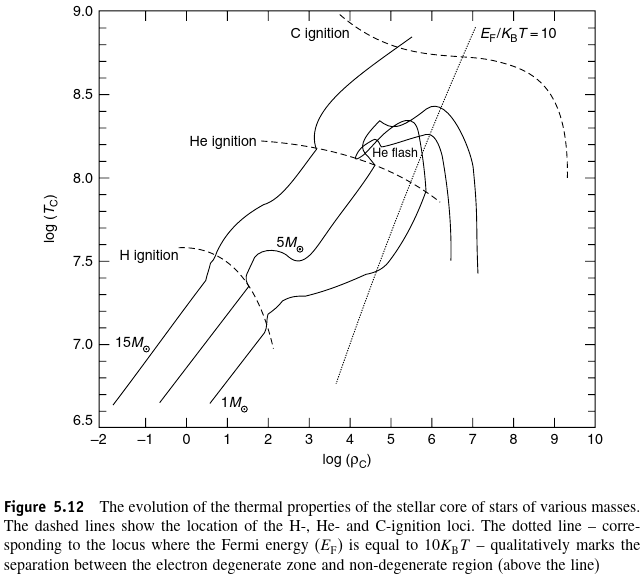
\includegraphics[trim={0cm 0cm 1cm 0cm},clip, keepaspectratio,height=0.3\textheight]{HHeCcore}\label{fig:HHeCcore}
\end{figure}
\begin{align*}
    &\Omega=-\alpha \frac{GM^2}{R}\\
    &\rho=\const:\alpha=\frac{3}{5}\\
    &E\approx \frac{3}{2}K\bar{T}\frac{M}{\mu m_H}\\
    &\Rightarrow\bar{T}\propto M^{\frac{2}{3}}\bar{\rho}^{-\frac{1}{3}}
\end{align*}
        \end{column}
    \end{columns}
\end{frame}

\begin{frame}{Condizione Core per fusione: virial theorem and degenerate electrons (SC: pg 59'- 103')}
    \begin{itemize}
        \item Electron degeneracy: $3(\gamma-1)$ is 2 (NR) or 1 (R) for degenerate \Pelectron; for mixture \Pelectron-ions $\gamma>\frac{4}{3}$. Case NR \Pelectron deg. $3(\gamma-1)=2$  (NR: $\gamma=\frac{5}{3}$): $\Omega=-2E=2E_{Tot}$, if $L=-\frac{1}{2}\TDy{t}{\Omega}$, $\Omega\propto \frac{1}{R}\propto\rho^{\frac{1}{3}}$ implica $\frac{1}{\Omega}\TDy{t}{\Omega}=\frac{1}{3}\frac{1}{\rho}\TDy{t}{\rho}$     
            \begin{align*}
                &n_e=\frac{\rho}{\mu_em_H}=\frac{8\pi p_F^3}{3h^3}\Rightarrow\rho\propto E_F^{\frac{3}{2}}\\
                &n(E_k)\,dE_k=\frac{8\sqrt{2}\pim_e^{\frac{3}{2}}}{h^3}E_k^{\frac{1}{2}}\,dE_k
                &E=\int_0^{E_F}n(E_{kin})E_{kin}\,dE_{kin}=\frac{1}{\rho}\int_0^{E_F}\frac{8\sqrt{2}\pi m_e^{\frac{3}{2}}}{h^3}E_{kin}^{\frac{3}{2}}\,dE_{kin}\propto \frac{1}{\rho}E_F^{\frac{5}{2}}\propto \frac{\rho^{\frac{5}{3}}}{\rho}\propto\rho^{\frac{2}{3}}\tag{Internal Energy per unit mass}\\
                &\Rightarrow \frac{1}{E_e}\TDy{t}{E_e}=\frac{2}{3}\frac{1}{\rho}\TDy{t}{\rho}\Rightarrow\TDy{t}{E_e}\approx2 \frac{E_e}{\Omega}\TDy{t}{\Omega}\\
        &\Omega=-2E, E=E_I+E_E\Rightarrow \Omega\approx-2E_e\tag{High degeneracy}\\
        &\TDy{t}{E_e}\approx2 \frac{E_e}{\Omega}\TDy{t}{\Omega}\Rightarrow\TDy{t}{E_e}\approx-\TDy{t}{\Omega}\\
        &L=-\TDy{t}{E_{tot}}=-\TDy{t}{E_e}-\TDy{t}{E_i}-\TDy{t}{\Omega}\approx-\TDy{t}{E_i}
            \end{align*}
    \end{itemize}
    Half gravitational energy not radiated away increases electron internal energy (Fermi energy), whereas ions thermal energy decreases. Evolution of degenerate object (WD) can be considered at constant radius $\Delta\Omega=\frac{\Delta R}{R^2}\approx L$
\end{frame}

\begin{frame}{SC-mass limit: upper limit to $M_c/M_{tot}$} 
    $\epsilon_n=0$ e gradiente radiativo implica formazione core di He isotermo(Energy transported by non degenerate electrons in analogy with photon diffusion is $F_e=-n_ev_el_e\TDy{r}{E}=-n_ev_el_e\TDy{r}{T}$, for degenerate electrons $l_e$ is much bigger $F=F_{rad}+F_e$): se la massa del core di elio \'e maggiore del $10\%$ della massa totale della stella il core si contrae - le stelle della LMS hanno core pi\'u piccolo, stelle di massa $M\geq2.5-3\msun{}$  hanno core pi\'u grande.
\begin{equation*} 
\frac{M_c}{M}>(\frac{M_c}{M})_{SC}=0.37(\frac{\mu_{env}}{\mu_c})^2\xrightarrow{\parbox{2.5cm}{$\mu_e=\mu_{\odot}=0.6$\\$\mu_c=\mu(He)=1.3$}}0.08
\end{equation*}
il core si contrae su $\tkh{}$.
Virial theorem for non-vanishing pressure surface pressure $P_0$ and $M_c$, $R_c$ and $T_c$:
\begin{align*}  
&(2U_i+\Omega+S_p=0,\ S_p=-\int\exv{v^2}\Vec{r}\cdot\hat{n}\,dS=P_0V)\\
&P_0=K_1\frac{M_cT_c}{R_c^3}-K_2\frac{M_c^2}{R_c^4}\tag{first term comes from Tot internal energy of core, second from grav. pot.}\\
&\frac{3}{2}\frac{K}{\mu m_u}T_cM\tag{total internal energy of core}\\
&P_{0,m}=K_3T_c^4/M_c^2\tag{Max $P_0$ for $R_c=\K_4\frac{M_c}{T_c}$}
\end{align*}
For equilibrium $P_{0,m}\geq P_e\propto M_T^2/R^4=T_c^4/M_T^2$ ($T_c\propto M_t/R$): therefore we have a limiti for $\frac{M_c}{M_T}$.
\end{frame}

\subsection{Intermediate, massive stars: He-ignition in non degenerate core ($M>2.3\msun{}$)}

\begin{frame}{Int-massive($M_*>2.3\msun{}$) stars: from SG to RG}
\begin{columns}[T]\begin{column}{0.5\textwidth}
\begin{figure}[!ht]
%trim: LBRT
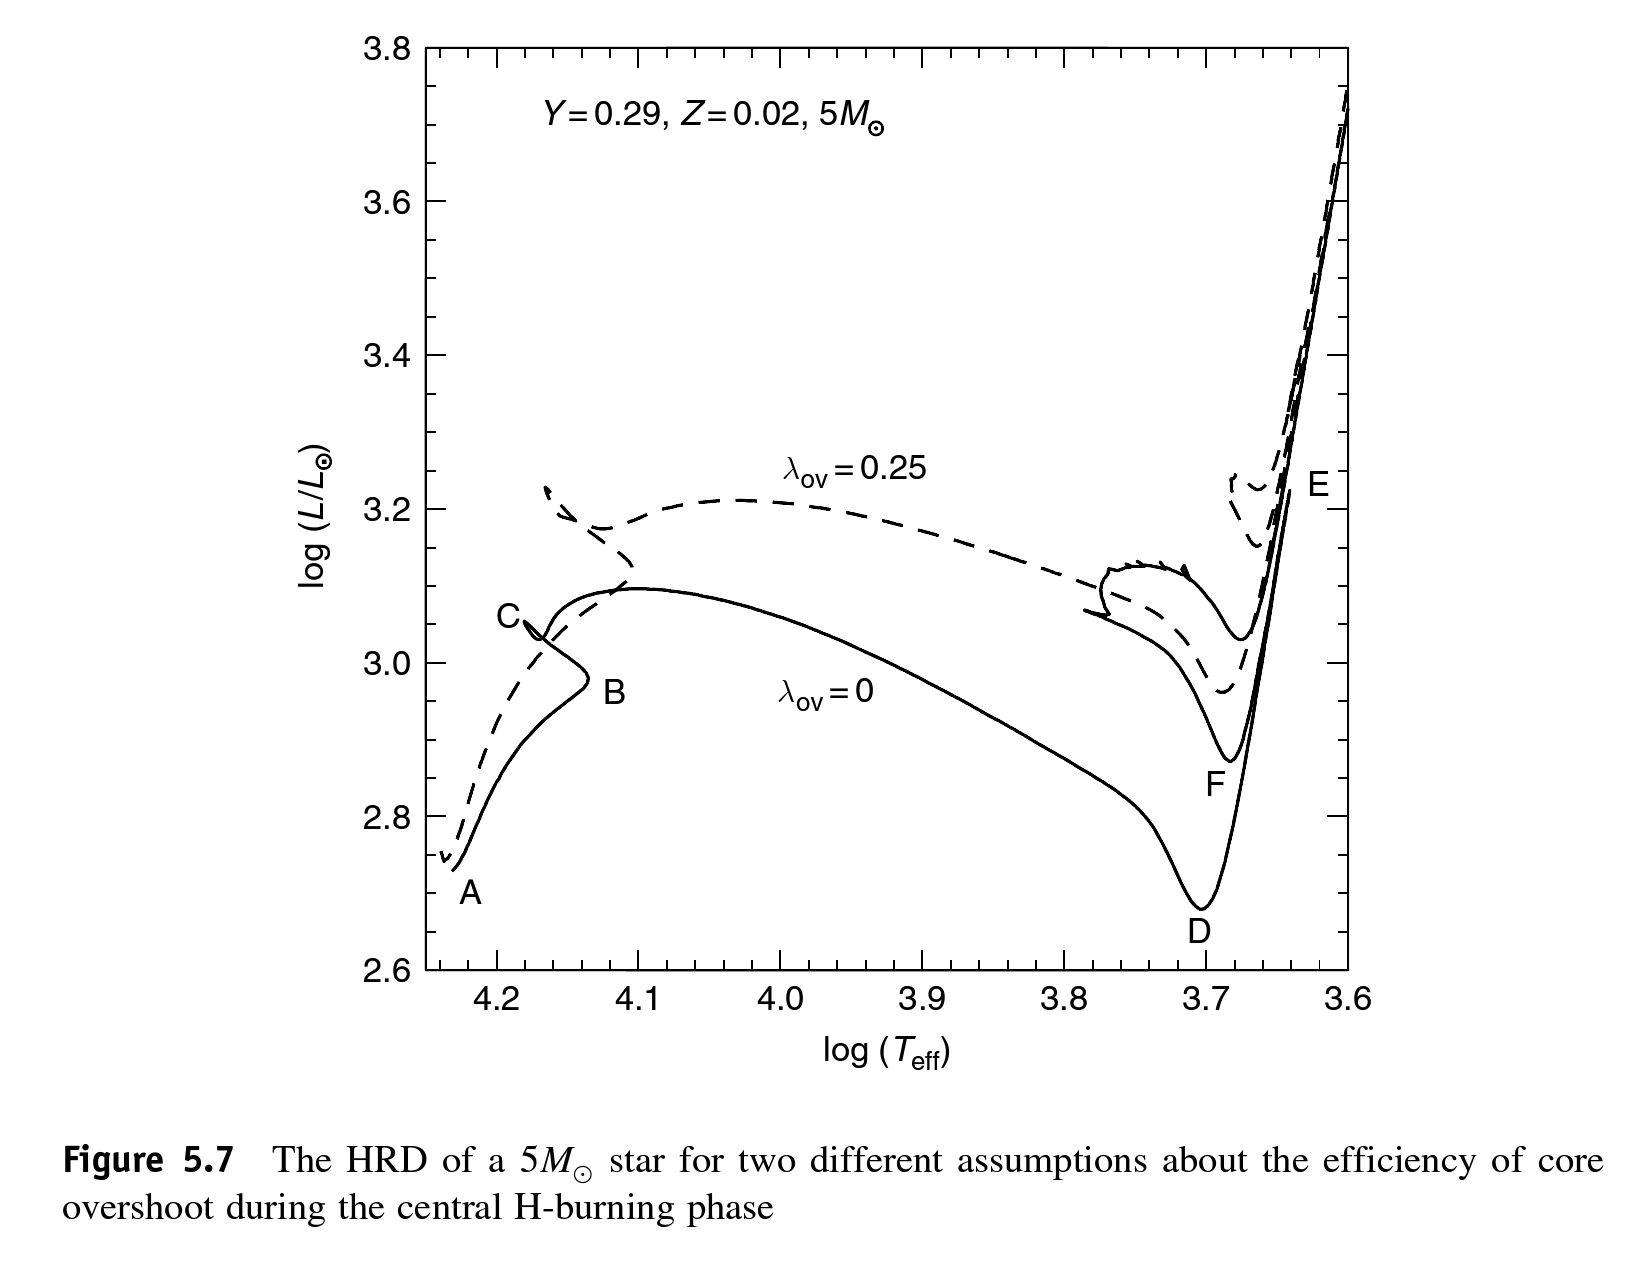
\includegraphics[trim={2.5cm 2cm 3.5cm 2.5cm},clip, keepaspectratio,width=0.99\textwidth]{HRD-overshoot}\label{fig:HRD-overshoot}
\end{figure}
\end{column}
\begin{column}{0.45\textwidth}
\begin{itemize}
    \item $M_c>M_{SC}$ (per $M\approx2.3-3$ limite superato dopo H-burning in shell): He core contract
    \item broad shell of CNO H-burning: $\epsilon_g$ changes sign at max $\epsilon_{CNO}$ - envelope expand: \xdiminuisce{T_e}, \xaumenta{\kappa_e} quindi inviluppo diventa convettivo.
    \item Star move from B to R at constant L - Hertzsprung gap: $\begin{array}{c}\tkh{}(3\msun{})\approx\SI{12}{\mega\year}\\\tkh{}(6\msun{})\approx\SI{1}{\mega\year}\end{array}$
\end{itemize}
\end{column}\end{columns}
\begin{itemize}
    \item In (D) star reaches Hayashi track where begins RG phase: $T_e$ costante, \xaumenta{L}. In (D) the stellar envelope becomes convective as it has cooled down during expansion: since it very efficient energy transport mechanism prevent slow down expansion.
    \item $\rho_c$ suff. low such onset of \Pelectron degeneracy is avoided: in (E) contracting core reaches $T\approx\SI{e8}{\kelvin}$ for efficient He-burning. \xaumenta{M_c} (VT: \xaumenta{T_c}) \xdiminuisce{\tau_{RG}}
\end{itemize}
\end{frame}

\subsection{Low-mass stars: He-flash and Dredge-up. Radiative core convective envelope.}

\begin{frame}{Low-mass stars}
    \begin{itemize}
        \item $M_{He,core}$ below SC limit and even when H-burning in shell produce bigger He-core the electron degeneracy provide support against contraction.
        \item $M_{cHe}-L$ relation: L provided by H-burning shell whose thermal prop are determined by He-core radius and mass.
        \item If evolving  at constant mass, Lower mass RGB stars at given L have larger radii and lower $T_{eff}$: mass loss shift star $T_e$ toward lower values.
        \item First dredge-up: as \xdiminuisce{T_e} during envelope expansion the convection goes deeper; Surface abundance of He monotonically increses as convection goes deeper as some of He produced in MS is mixed in; also $^3He$ and CNO elements are mixed.
        \item RGB bump: along RGB convection receeds as H-burning shell moves outward and when H-burning shell encounter discontinuity have peculiar behaviour in that region of HRD (\xaumenta{X},\xdiminuisce{T},\xdiminuisce{L}: $L_H\propto\mu^7$)- stars stay $20\%$ of RGB lifetime in region of HRD.
        \item Max T moves outside center in He core: for $M_r\leq0.3M_T$: $\epsilon_g+\epsilon_{\nu}<0$, $\TDy{r}{L}<0$ near center so develope T-inversion.
        \item He ignited when $M_{cHe}\approx0.5\msun{}$ in shell around degenerate core.
        \item Thermal runaway at Tip of RGB: He-flash.
    \end{itemize}
\end{frame}

%trim: LBRT
\begin{frame} {Low-mass stars: nuclear burning changing after X exhaustion in the center}
\begin{columns}[T]\begin{column}{0.5\textwidth}
\begin{figure}[!ht]
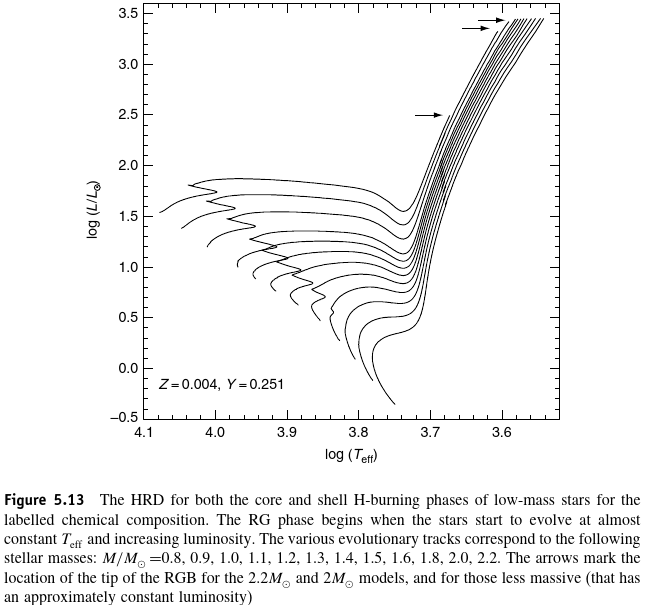
\includegraphics[trim={0cm 0cm 0cm 0cm},clip, keepaspectratio,width=0.99\textwidth]{HDRtipRGB}\label{fig:HDRtipRGB}
\end{figure}
\end{column}
\begin{column}{0.4\textwidth}
\begin{itemize}
\item As X exhausts max $\epsilon_H$ is no more in central region (at TO at $M_r=0.1\msun{}$). He Core (radiative/small convective??): $M<M_{SC}$, high electron degeneracy.
\item From TO to RG H-burning shell becomes thinner due to CNO deps on T that decreses in envelop and H depleted in inner portion rapidly.
\end{itemize}
\end{column}\end{columns}
\begin{itemize}
\item $M_{cHe}-L$ relation: \xaumenta{M_{cHe}}, \xaumenta{L}. L is almost fully provided by H-burning shell whose thermal properties are determined $R_c$, $M_c$ ($P_e$ is OM lower)
%\item RGB stars evolve at constant L and radius re-adjust to stellar mass: mass loss shift $T_e$ toward lower values.
\end{itemize}
\end{frame}

\begin{frame}{Envelope structure: depth of convection and first dredge-up}
\begin{columns}[T]\begin{column}{0.44\textwidth}
%trim: LBRT
\begin{figure}[!ht] 
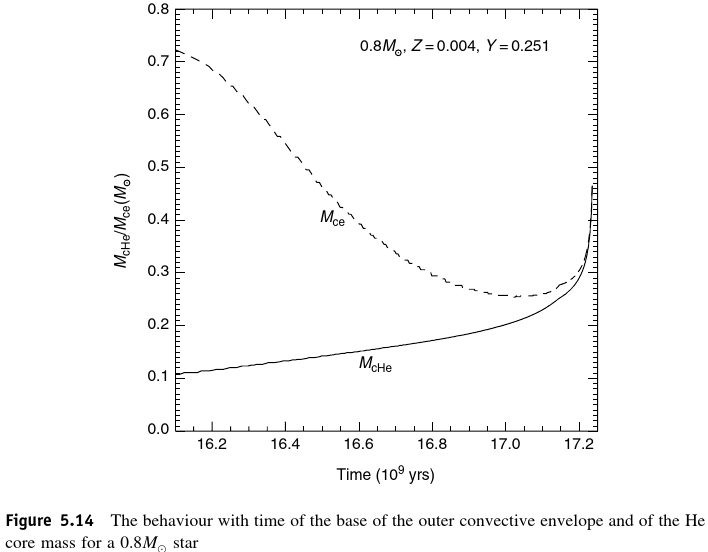
\includegraphics[trim={0cm 0cm 0cm 0cm},clip, keepaspectratio,height=0.45\textheight]{postMS-depthC}\label{fig:postMS-depthC}
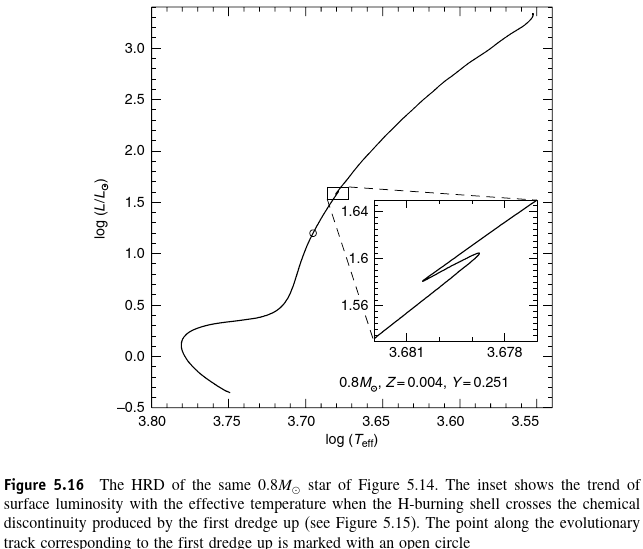
\includegraphics[trim={0cm 0cm 0cm 0cm},clip, keepaspectratio,height=0.45\textheight]{HburnxIdu}\label{fig:HburnxIdu}
\end{figure}
\end{column}
\begin{column}{0.50\textwidth}
\begin{itemize}
\item Cooling  of envelop causes deeper convection that reaches a maximum before RG (\xdiminuisce{T}, \xaumenta{\kappa}). Primo dredge-up: \xaumenta{He_s}, \xaumenta{^{14}N_s}, \xdiminuisce{^{12}C} ($\frac{^{12}C}{^{13}C}$), $Li$, $Be$ reduces several OM.
\item In  RGB phase H-burning shell move outward and convective zone move toward surface: chemical discontinuity at max convective depth. \keyword{Bump of RGB}: as H-burning shell meet discontinuity $L_H\propto\mu^7$ diminish in the fully mixed envelop \xaumenta{L} as \xaumenta{M_{cHe}} - bump in RGB luminosity function ($20\%$ rgb-time in this luminosity range)
\end{itemize}


\begin{figure}[!ht] 
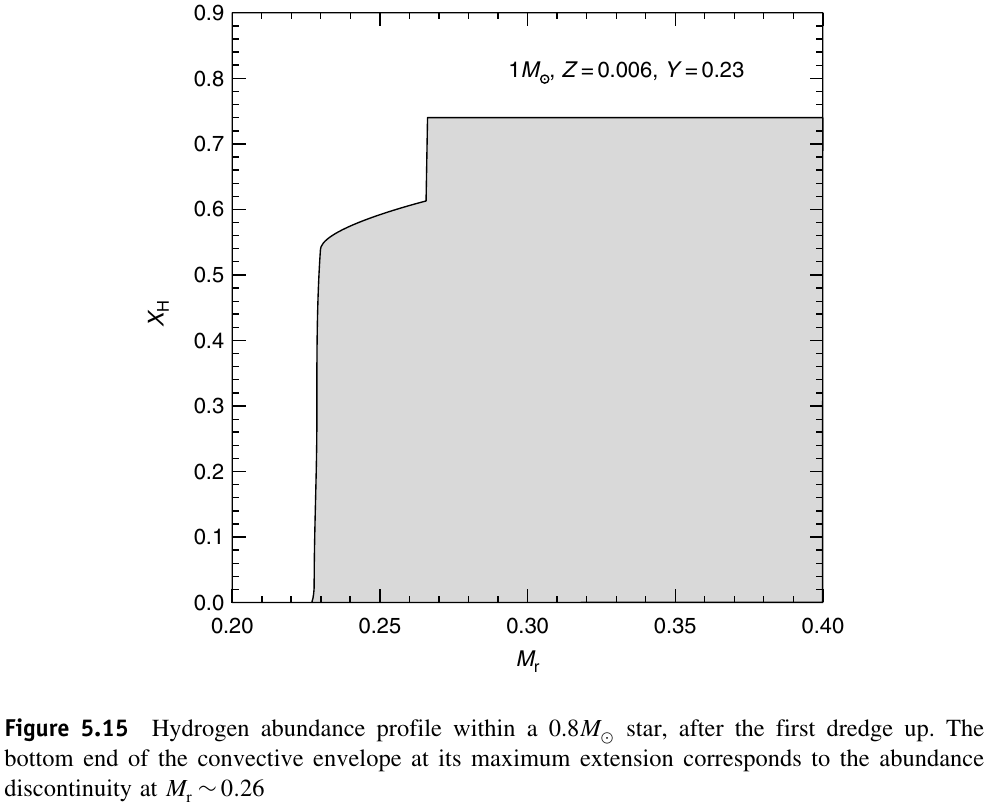
\includegraphics[trim={0cm 0cm 0cm 0cm},clip, keepaspectratio,height=0.45\textheight]{dredgedup-X}\label{fig:dredgedup-X}
\end{figure}
\end{column}\end{columns}
\end{frame}

\begin{frame}{\keyword{Thermal runaway at tip of RGB}: He-flashes}
\begin{columns}[T]\begin{column}{0.48\textwidth}
%trim: LBRT
\begin{figure}[!ht]
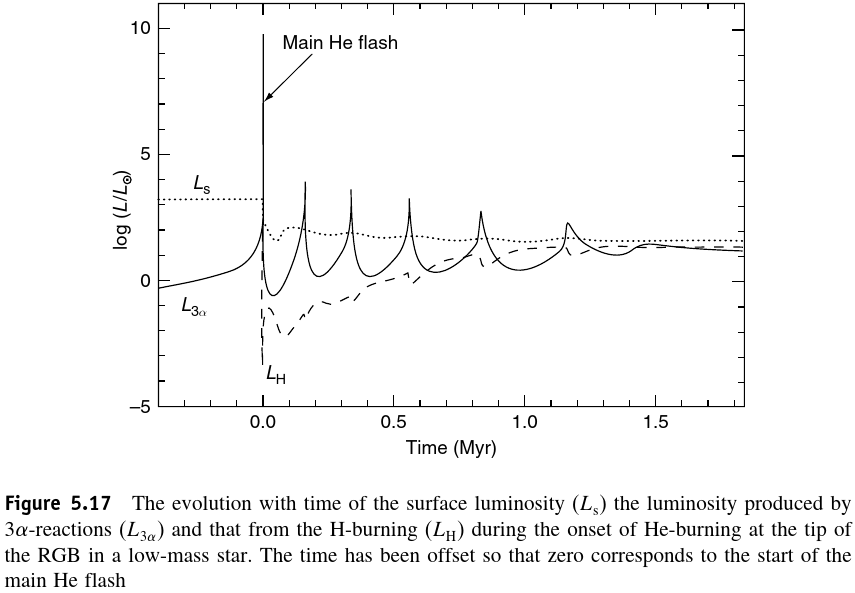
\includegraphics[trim={0cm 0cm 1cm 0cm},clip, keepaspectratio,width=0.99\textwidth]{He-flash}\label{fig:He-flash}
\end{figure}
\end{column}
\begin{column}{0.43\textwidth}
    In RG phase: H-burning increases $M_{cHe}$ and \xaumenta{\rho_c}. In inner part $M_r<0.3M_t$ when $\epsilon_g+\epsilon_{\nu}<0$: $\TDy{r}{L}<0$ resulting in T-inversion. \xaumenta{\rho_c}, grado di degenerazione aumenta, \xdiminuisce{\kappa_{cond}}, \xdiminuisce{T_c} (strong degeneracy: $\kappa_{cd}\propto\rho^{-2}T^2$); while \xaumenta{T_c^M} due to $\epsilon_g>0$ at boundary between D/ND matter. At $T_c^M\approx\SI{e8}{\kelvin}$ we have He ignition ($M_{cHe}\approx0.48-0.5\msun{}$): end of RGB phase.
\end{column}\end{columns}
He ignition at strong partial-relativistic-D ($\rho_x\approx\SI{e6}{\gram\per\cubic\cm}$, $T\approx\SI{8e7}{\kelvin}$), $P$ is insensitive to $T$ changes, rate of $3\alpha$-burning increases much: thermal runaway $\num{e10}\lsun{}$ in few seconds are absorbed by above ND layers: expansion and convection (large jump in P/S prevent mixing with above H-burning). So \xaumenta{T_c} at constant $\rho$ but no time for heat diffuse the whole core: this need many successive He-flashes, $\tau_{flash}\approx\SI{e6}{\year}$ and $5\%$ He converted to C
\end{frame}

\subsection{Deps of RGB on params}\linkdest{depsRGB}

\begin{frame}{Location of RGB on HRD}
\begin{itemize}
    \item Highly Z-dependent: size of convective envelop (Hayashy track) \xaumenta{Z}, \xaumenta{\kappa}, inviluppo convettivo pi\'u grande. Abundance of low ionization potential elements (Mg, Si, S, Ca, Ti, Fe) influence RGB $T_e$ through molecule $TiO$ and releasing \Pelectron to form$H^-$: $\alpha$-enhanced star has RGB cooler and less steeper, change in slope is due to increasing contribute of molecules to envelope opacity as $T_e$ decreases.
\item \xaumenta{Y}, \xdiminuisce{\kappa}, \xdiminuisce{CE}, \xaumenta{T_e}
\item RGB is important Z indicator of galaxies/star clusters
\item $\rho_e$ low: $\nabla_e$ \'e super-adiabatico (\xaumenta{
\alpha_{ML}},\xaumenta{T_e})
\item \keyword{RGB phase transition}. Luminosity of Tip-RGB is function of $M_{cHe}$ at He-flash: \xaumenta{L_{Tip}} \xaumenta{M_{cHe}}. 

    \xdiminuisce{M_*}, \xdiminuisce{T_e}: $M_{cHe}$ constant for $M\leq1.8\msun{}$ (this limit deps on composition, here solar) developing similar level of degeneracy so havin similar $M_{cHe}$ then \xdiminuisce{M_{cHe}}, \xaumenta{M} as \xaumenta{M}, \xaumenta{T_c}, \xdiminuisce{\rho_c} produce lower level of degeneracy, then reaching minimum $M_{cHe}$ increases with M, degeneracy is totally removed, as a consequence of larger convective core during H-burning.
\end{itemize}
\end{frame}

\begin{frame}{Luminosity of RGB bump: earlier shell hit discontinuity lower L}
\begin{columns}[T]\begin{column}{0.52\textwidth}
%trim: LBRT
\begin{figure}[!ht]
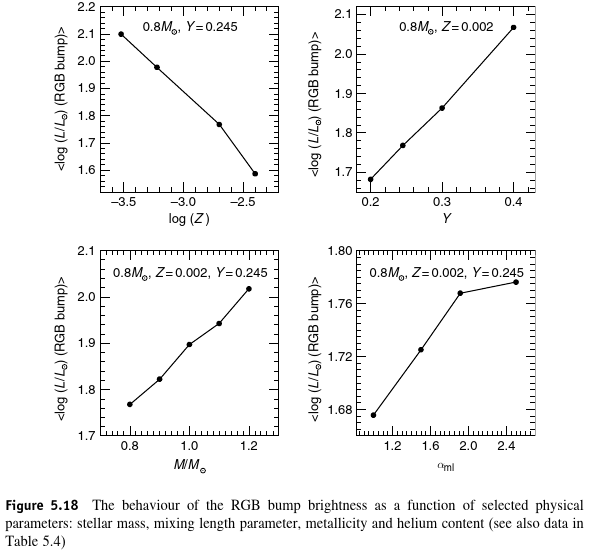
\includegraphics[trim={0cm 0cm 1cm 0cm},clip, keepaspectratio,width=0.99\textwidth]{RGB-bumpparams}\label{fig:RGB-bumpparams}
\end{figure}
\end{column}
\begin{column}{0.43\textwidth}
    As convection zone goes deeper the H-burning shell takes less time to cross chemical discontinuity and surface luminosity is lower: (\xdiminuisce{M_*}/\xaumenta{Z}/\xdiminuisce{Y},\xdiminuisce{\alpha_{ML}}), \xdiminuisce{L_{bump}}.
    \begin{itemize}
        \item He decrease or Z increases, due to chenges of envelope's opacity, move discontinuity deeper reducing L-bump
        \item Large convection efficency ($\alpha$) decreases mass extension of outer convection zone at first dredge-up: discontinuity is more external so L-bump higher.
    \end{itemize}
\end{column}\end{columns}
\end{frame}

\begin{frame}{Deps RGB tip's (He-ignition) luminosity on params}
\begin{columns}[T]\begin{column}{0.5\textwidth}
%trim: LBRT
\begin{figure}[!ht]
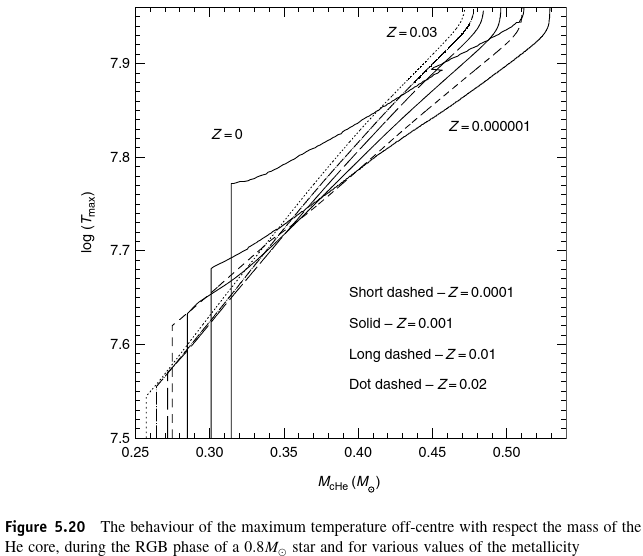
\includegraphics[trim={0cm 0cm 1cm 0cm},clip, keepaspectratio,height=0.36\textheight]{RGBTmax}\label{fig:RGBTmax}
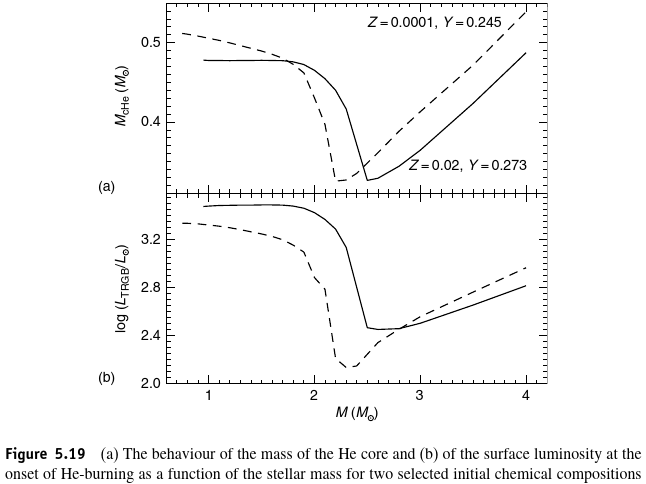
\includegraphics[trim={0cm 0cm 1cm 0cm},clip, keepaspectratio,height=0.36\textheight]{HecLsatHeburning}\label{fig:HecLsatHeburning}
\end{figure}
\end{column}
\begin{column}{0.45\textwidth}
\begin{itemize}
    \item \keyword{RGB phase transition}. \xdiminuisce{M_*}, \xdiminuisce{T_e}: $M_{cHe}$ constant for $M\leq1.8\msun{}$ then decreases with $M$ as degeneracy is completely removed then increases as consequences of larger convective H-burning core.
    \item \xaumenta{He}, \xaumenta{T_c}, deg \Pelectron diminuisce, $M_{cHe}$ He-ignition diminuisce, \xdiminuisce{L_{TIP}}
    \item \xaumenta{Z}, \xaumenta{\epsilon_{CNO}}, $M_{cHe}$-ignition is builded faster since He production by H-burning shell is faster and He-core growth, hence heating, is faster: thermal conditions for He-ignition reached at lower $M_{cHe}$. \xdiminuisce{L_{TIP}}.
    \item At odds with prev point with increasing Z, regardless of $M_{cHe}$ at tip RGB, L at He-ignition increases: $M_{cHe}-L$ affected by initial chemical composition \xaumenta{Z}, \xaumenta{\epsilon_H^{shell}}, so increases also surface luminosity at each fixed value of $M_{cHe}$
\end{itemize}
\end{column}\end{columns}
\end{frame}

\subsection{Very low Z stars}\linkdest{lowz}

\begin{frame}{Very low Z (pop III)}
\begin{itemize}
    \item Primordial star (Pop III) responsable for Z-enrichment: from $Z\approx\numrange{e-10}{e-12}$ to $Z\approx\numrange{e-2}{e-3}$ (Pop II)
    \item High mass star burn H through PP chain so need much higher T; as $T\approx\SI{e8}{\kelvin}$ He-burning produce $^{12}C$: threshold for CNO H-burning to begins $X_C\approx\numrange{e-9}{e-10}$
    \item \xaumenta{M_*}, \xdiminuisce{\tau_{PP\to CNO}}: transition to convective core for $M>2\msun{}$ (for $M=2-5\msun{}$ convective core after $^3He$ production phase).
    \item RGB phase transition at lower mass/higher age: for low mass star \xaumenta{T_c} due to low, degenerazione elettronica del core di He diminuisce, faster He ignition, \xdiminuisce{M_{cHe}}, \xdiminuisce{L_{TIP}}
    \item Intermediate mass star have no RGB
\end{itemize}
\begin{columns}[T]
    \begin{column}{0.5\textwidth}
        \begin{figure}[!ht] 
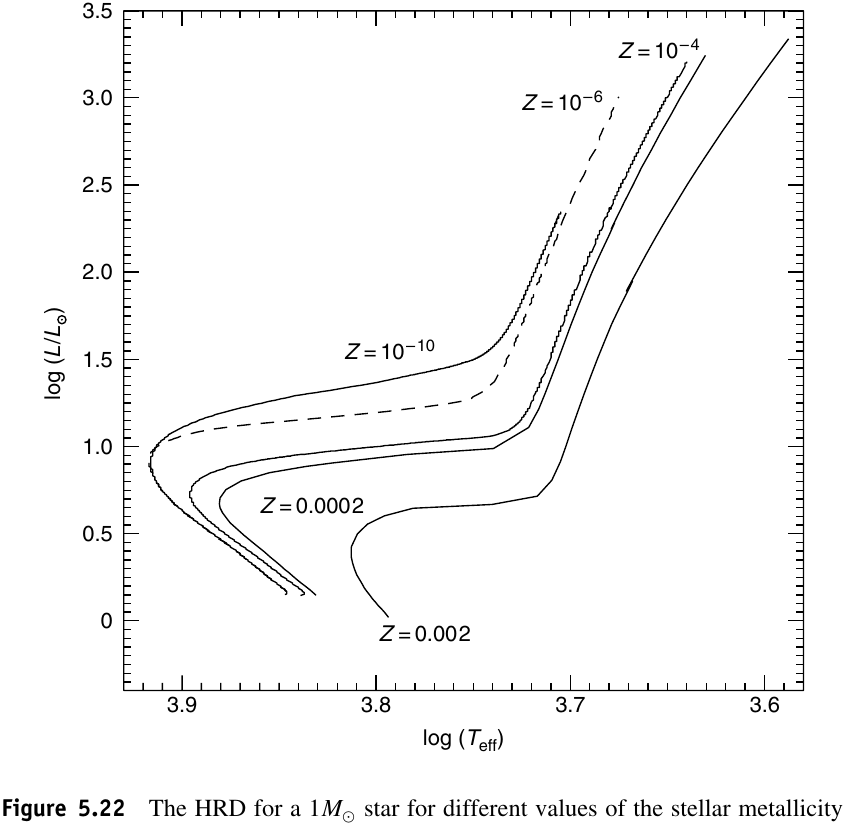
\includegraphics[trim={0cm 0cm 0cm 0cm},clip, keepaspectratio,width=0.85\textwidth]{lowZ1MsunHDR}\label{fig:lowZ1MsunHDR}
\end{figure}
    \end{column}
    \begin{column}{0.5\textwidth}
        \begin{figure}[!ht] 
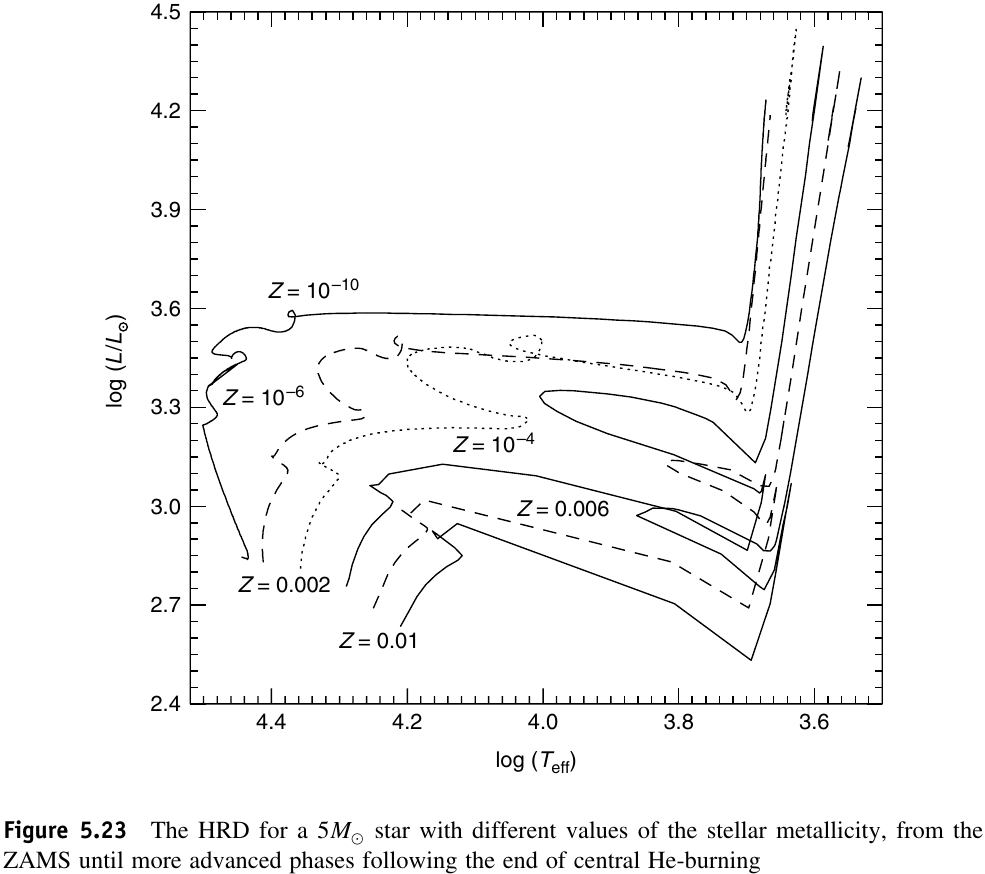
\includegraphics[trim={0cm 0cm 0cm 0cm},clip, keepaspectratio,width=0.85\textwidth]{lowZ5MsunHDR}\label{fig:lowZ5MsunHDR}
\end{figure}
    \end{column}
\end{columns}

\end{frame}

\subsection{Refs. HB}

\begin{frame}{Memo per HB}
combustion di He per stelle medio-grandi; clump He; loop He; Esaurimento He centrale: , semiconvezione e pulsi convettivi
\end{frame}

\subsection{He-burning reactions}

\begin{frame}{He-burning reactions}
\begin{columns}[T]\begin{column}{0.45\textwidth}
	\begin{align*}
&3\alpha (T\gtrsim\SI{1.2e8}{\kelvin}):\\ &^4He+^4He\to^8Be\tag*{$\tau_{1/2}\approx\SI{e-16}{\second}$}\\
&^8Be+^4He\to^{12}C+\gamma\tag*{$\SI{7.27}{\mega\ev}$, $\tau_H\approx100\tau_{He}$}\\
&\epsilon_{3\alpha}\approx\begin{array}{c}Y^3\rho^2T^{40}: T\approx\SI{e8}{\kelvin}\\T^{20}: T\approx\SI{2e8}{\kelvin}\end{array}
\end{align*}
Energy release per gram $Q/m(^{12}C)=\SI{5.9e17}{\erg\per\gram}$ - $1/10$ di quella prodotta da H-burning
	\end{column}
	\begin{column}{0.40\textwidth}
	\begin{align*}
&^{12}C+\alpha\to^{16}O+\gamma\tag*{Q=\SI{7.162}{\mega\ev}}\\
&^{16}O+\alpha\to^{20}Ne+\gamma\\
&^{20}Ne+\alpha\to^{24}Mg+\gamma\\
&^{24}Mg+\alpha\to^{28}Si+\gamma
\end{align*}
$\epsilon_{\alpha C}\propto YX_{12}\rho T^{20}$
\end{column}\end{columns}
\end{frame}

\subsection{Equilibrium model for low mass star after He-flashes: ZAHB}\linkdest{ZAHB}

\begin{frame}{Low Mass star HB: Flash-pulses to ZAHB and evolution from ZAHB}
    \begin{columns}[T]
        \begin{column}{0.55\textwidth}
\begin{figure}[!ht]
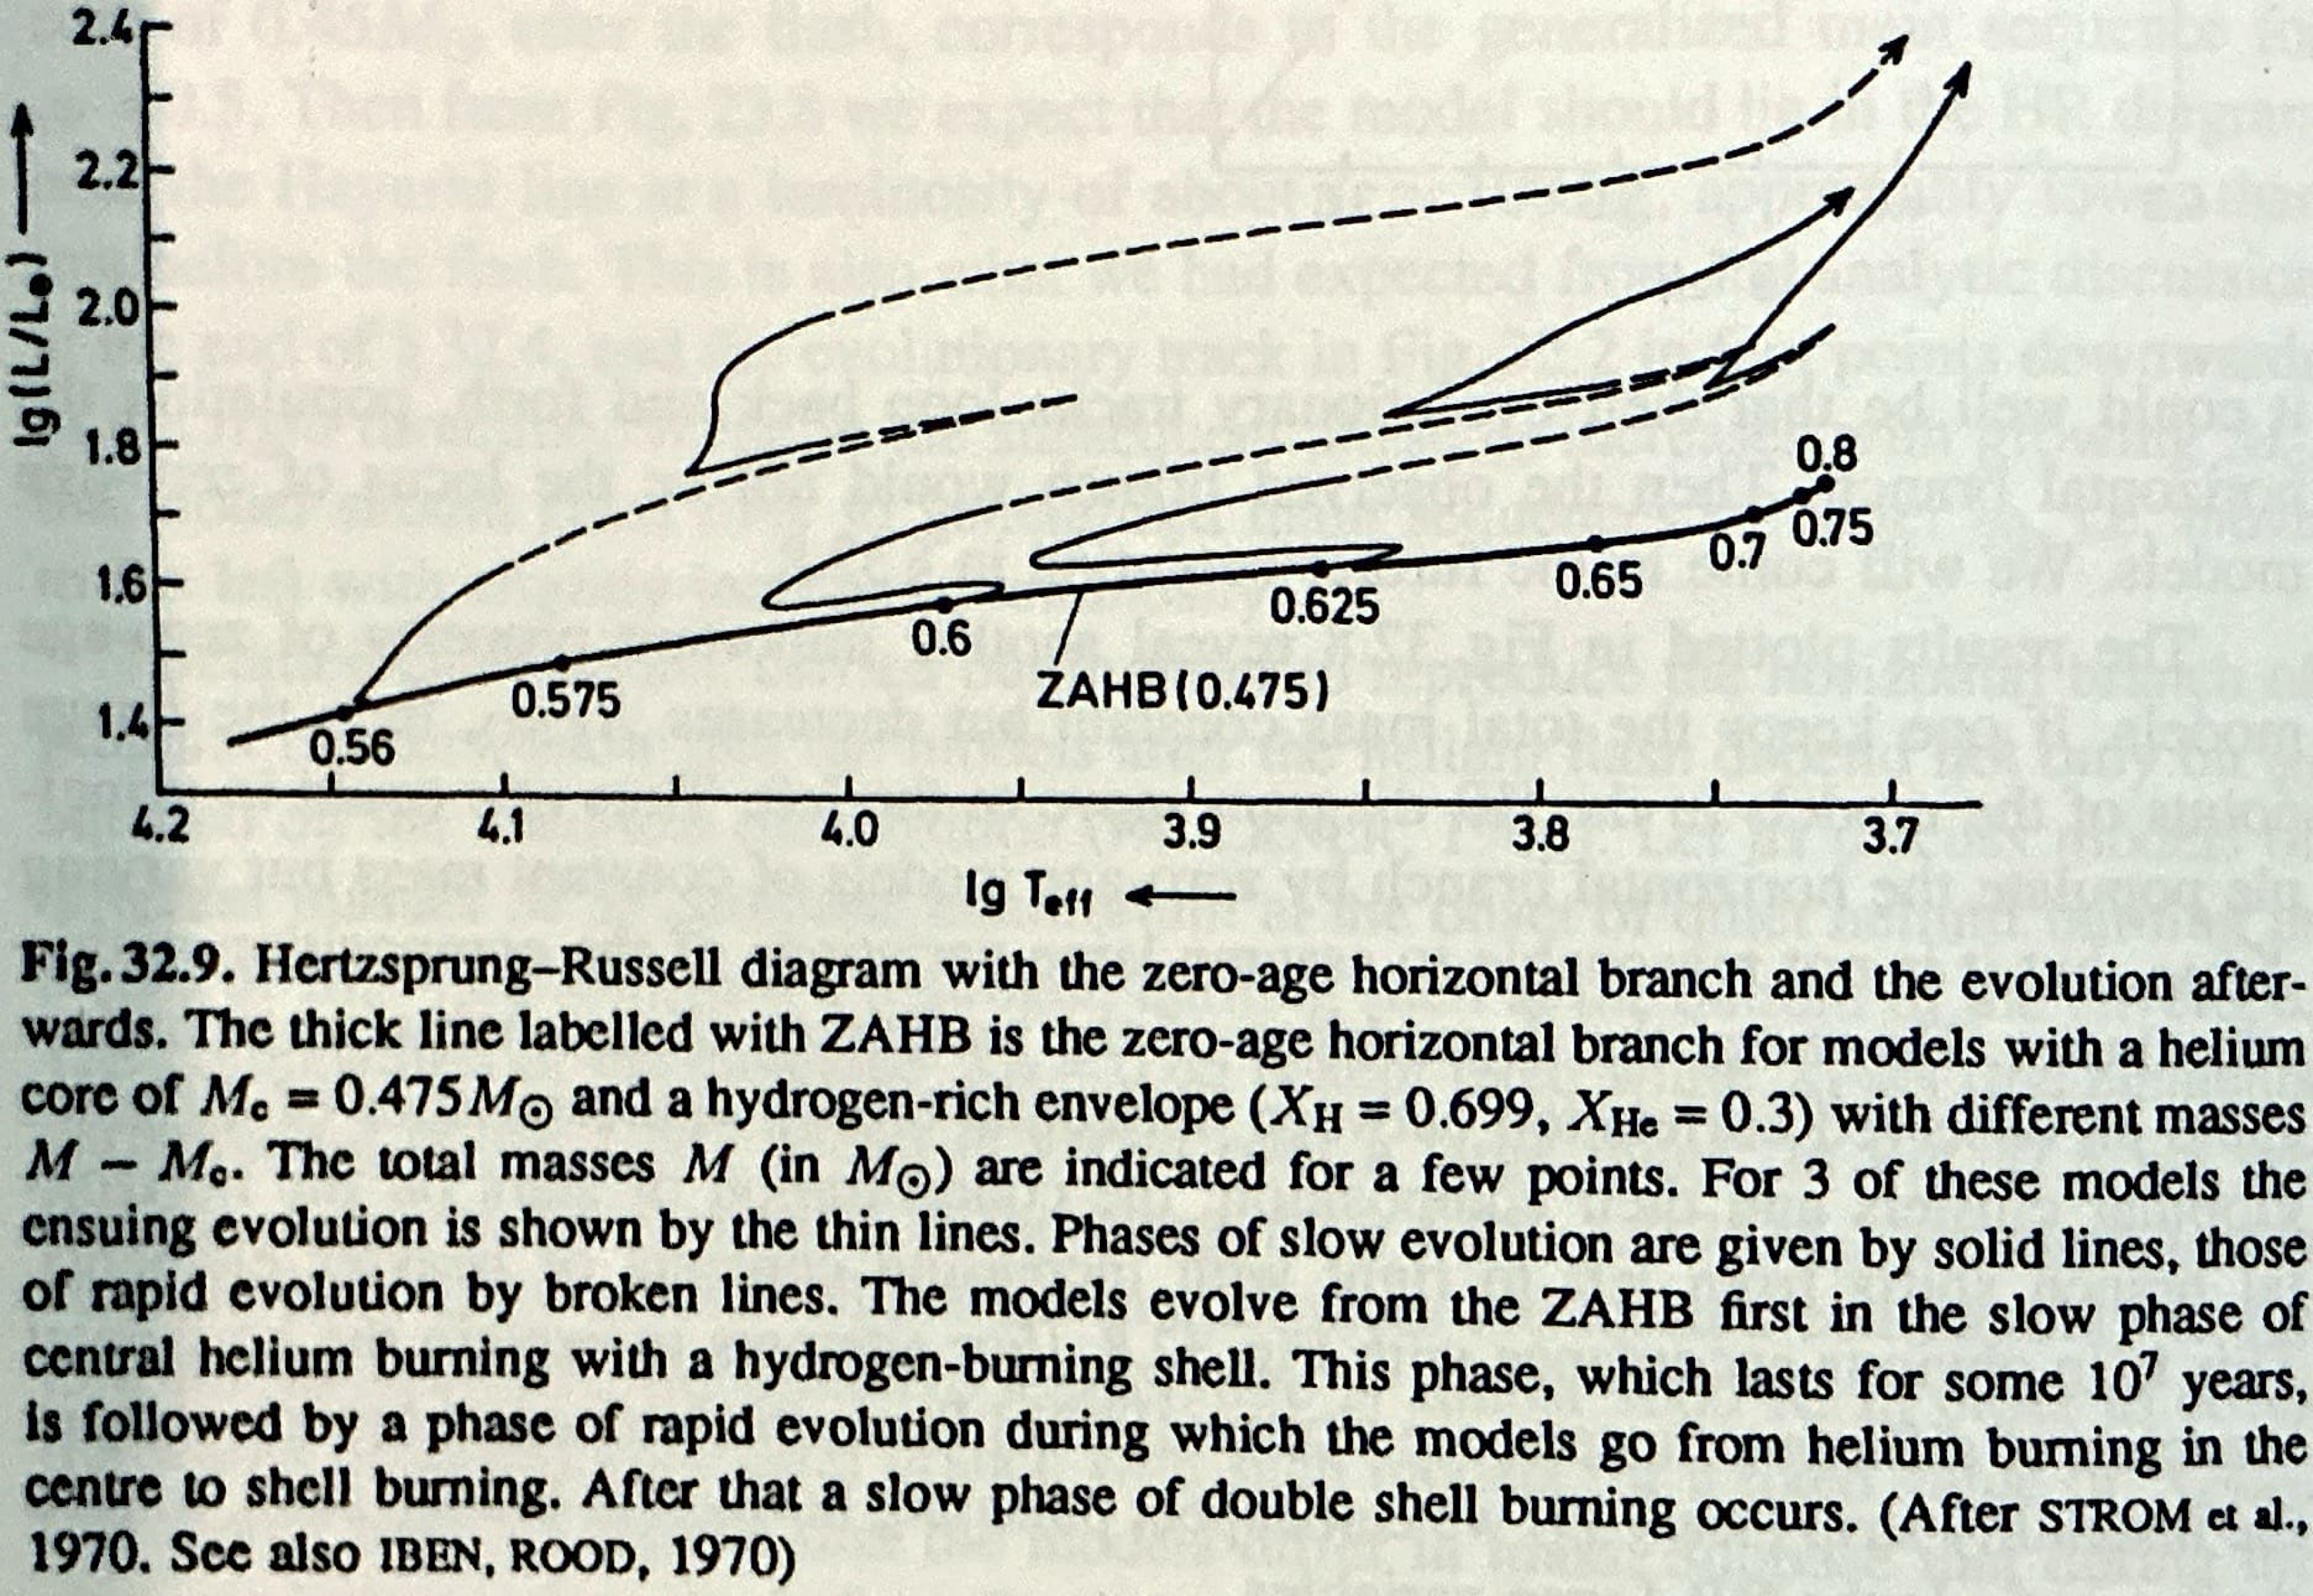
\includegraphics[trim={0cm 0cm 0cm 0cm},clip, keepaspectratio,width=0.75\textwidth]{evolfromZAHB}\label{fig:evolfromZAHB}
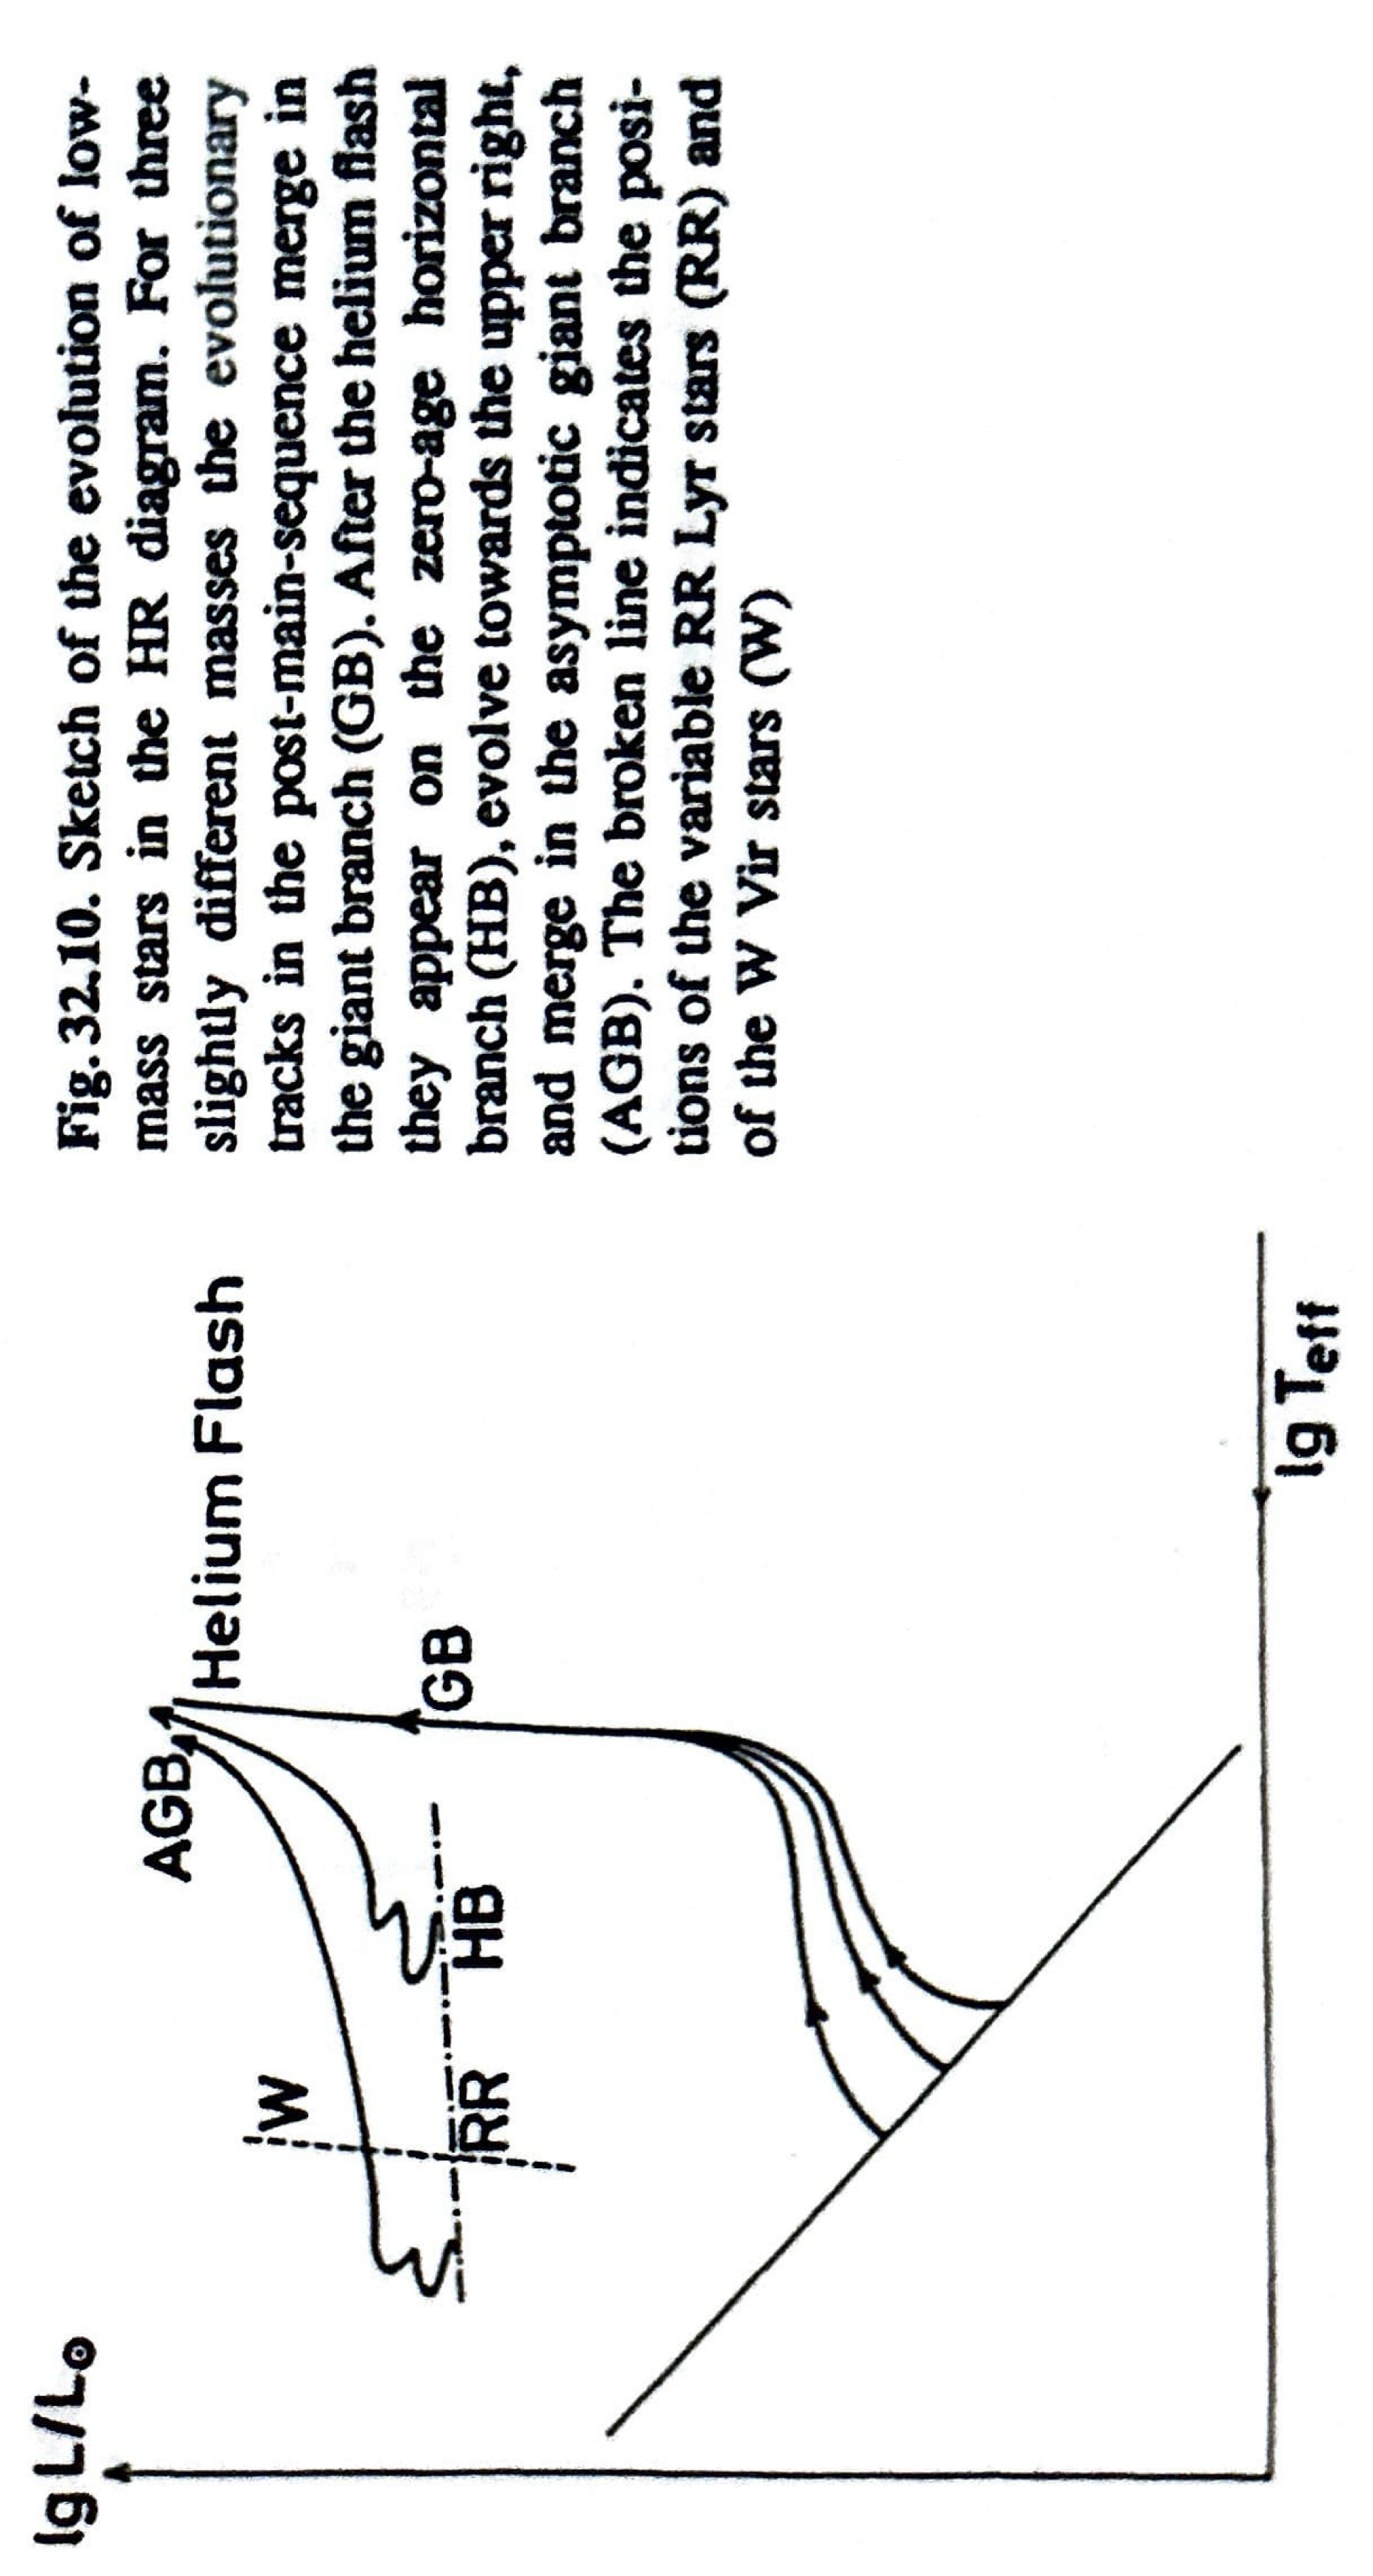
\includegraphics[trim={0cm 0cm 0cm 0cm},clip, keepaspectratio,height=0.75\textheight,origin=c,angle=-90]{Heflash2ZAHB}\label{fig:Heflash2ZAHB}
\end{figure}
        \end{column}
        \begin{column}{0.45\textwidth}
            \begin{itemize}
                \item He-pulses remove \Pelectron-deg from He-core: L drops 1 OM resp tip-RGB as core heating and expanding causes H-burning shell to cool down.
                \item Evolution from tip-RGB to He-burning very short: observing prob quite zero so many calculations begins from equilibrium model.
                \end{itemize}
        \end{column}
    \end{columns}
    
\end{frame}

\begin{frame}{ZAHB: equilibrium model} 
\begin{itemize}
    \item $\tau_{He-Flash}\approx\SI{e6}{\year}$: after that time of He-burning the \Pelectron degeneracy is removed (small obser. prob). Some authors start He-core evolution sequence from C enriched equilibrium model (C enrichment about $5\%$).
\item \keyword{ZAHB}: model where He is burnt into chem homo-core and H in shell with chem stratification He-flash like
\item He-enriched by I dredge-up: $\Delta Y\approx\numrange{0.02}{0.04}$.
\item Rotation (dalayed He-flash): \xaumenta{M_{cHe}}, \xdiminuisce{M_*} (mass loss), \xaumenta{T^{ZAHB}}/\xaumenta{L^{ZAHB}}
%\xaumenta{\epsilon_{He}}/\xdiminuisce{\epsilon_H}
\end{itemize}
\end{frame}

\begin{frame}{Another ZAHB ??}
\begin{columns}[T]
	\begin{column}{0.45\textwidth}
	\end{column}
	\begin{column}{0.45\textwidth}
		\begin{figure}[!ht]
			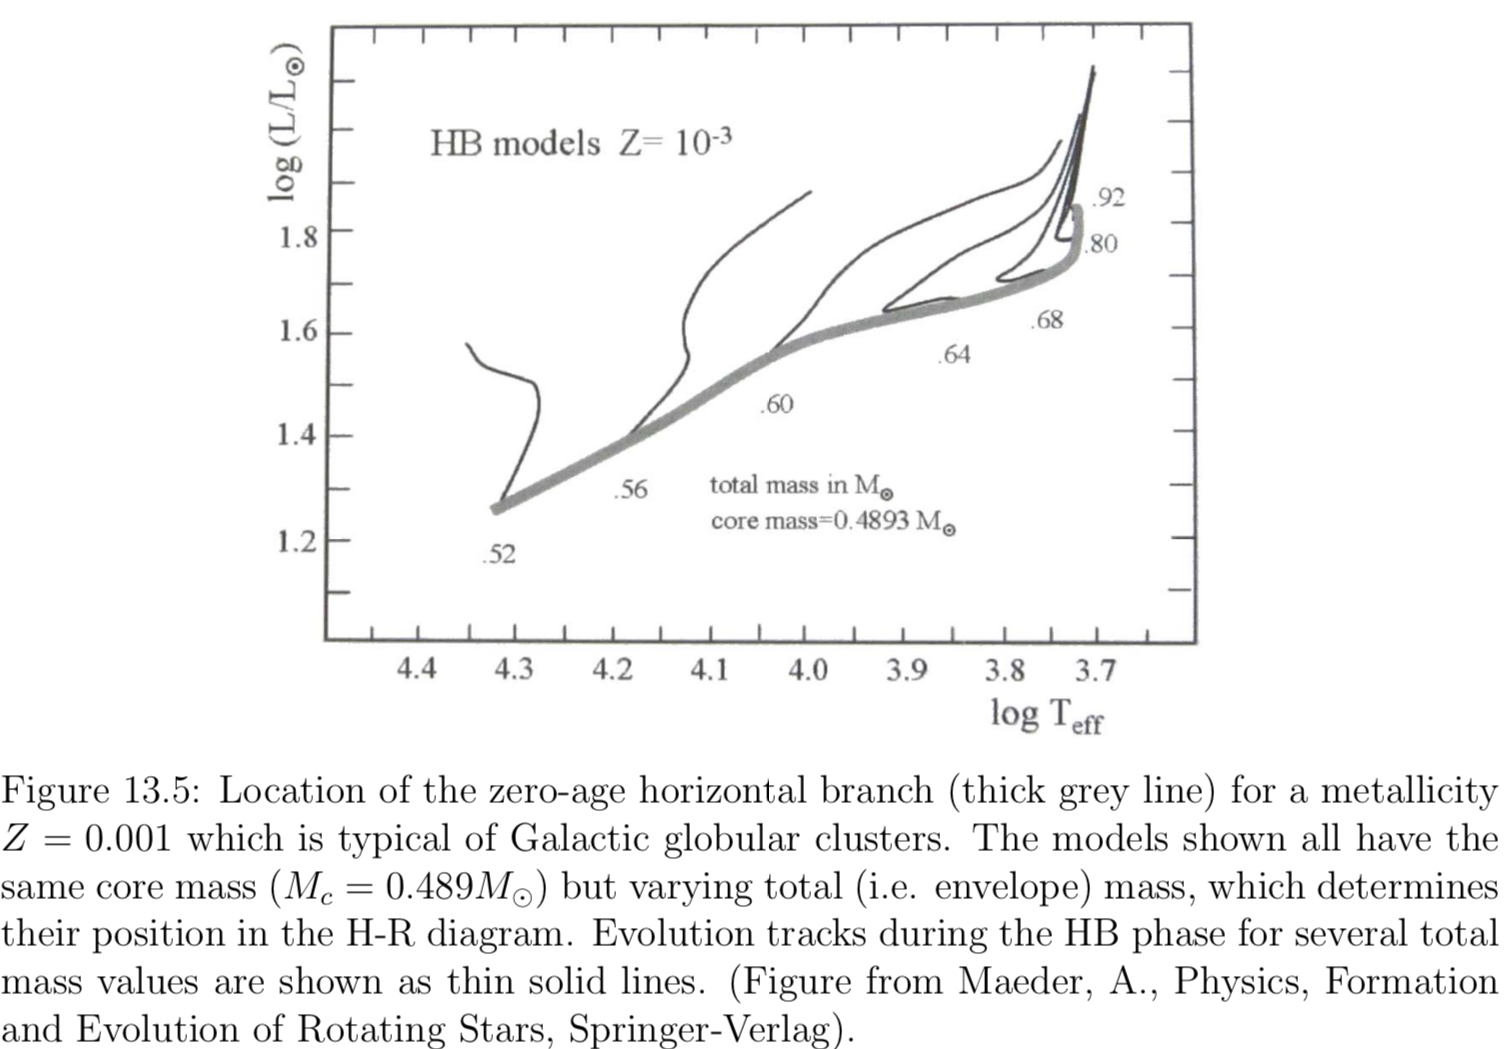
\includegraphics[trim={0cm 0cm 1cm 0cm},clip, keepaspectratio,height=0.37\textheight]{HB-ZA-evol}\label{fig:HB-ZA-evol}
		\end{figure}
	\end{column}
\end{columns}
\end{frame}

\begin{frame}{ZAHB dep on core (and  envelope) mass}
\begin{itemize}
\item Structure and evolution of ZAHB  fixed by: $M_*$, $M_{cHe}$ (for $M<1.8\msun{}$ $t_{TIP}>4-5\si{\giga\year}$: $M_c$ weakly dependent on M), $Y$, $Z_e$ - for low mass progenitors ZAHB is determined by Y, Z abundances of envelope and total mass - For fixed composition, $L_s$ is fixed by $M_{cHe}$ (then by $M_e$): important standard candles for Pop II stars (\keyword{Standard candles: HB brightness}). $(\TDy{M_{cHe}}{\log{L_{ZAHB}^{\log{T_e}=3.85}}})_{Y,Z}\approx3.04$
\item Location in HDR: \xdiminuisce{M_e }, \xaumenta{T_e} - HB (slightly oblique due to \xaumenta{\epsilon_H},\xaumenta{M_e}). $T_e\approx\SIrange{3500}{4000}{\kelvin}$ for $M_e\approx\numrange{e-4}{0.4}\msun{}$ (RGB mass loss)
\item \xaumenta{R_{cHe}}, \xdiminuisce{L_s} from RGB-tip as H-burning shell cool down
\item He-burning in convective core (steep T deps)
\item H-burning in shell: for fixed $M_{cHe}$ efficiency determined by \xaumenta{M_e}, \xaumenta{\epsilon_H}
\item HB-Brightness on of most important standard candles for PopII stars: L mainly fixed by $M_{cHe}$.
\end{itemize}
\end{frame}

\begin{frame}{ZAHB dep on composition}
\begin{columns}[T]
\begin{column}{0.55\textwidth}
\begin{itemize}
    \item \xaumenta{Y_{in}}, \xdiminuisce{M_{cHe}}, \xaumenta{L_H}/\xdiminuisce{L_{cHe}}, $L^{ZAHB}$ approx const: Blue (low mass envelope) part of ZAHB becomes fainter/ R part brighter. $(\TDy{Y}{L_{ZAHB}^{3.85}})_{M_{cHe},Z}\approx2.07$
\item \xaumenta{Z_{in}}, \xdiminuisce{M_{cHe}^{Flash}}/\xaumenta{\kappa_e}, \xdiminuisce{L^{ZAHB}}/\xdiminuisce{T_e^{ZAHB}}. $(\TDy{Z}{L_{ZAHB}^{3.85}})_{M_{cHe},Y}\approx-0.04$
\end{itemize}
\end{column}
\begin{column}{0.45\textwidth}
\begin{figure}[!ht]
\includegraphics[trim={0cm 0cm 0cm 0cm},clip, keepaspectratio,height=0.37\textheight]{HDR-ZAHB-M08}\label{fig:HDR-ZAHB-M08}
\includegraphics[trim={0cm 0cm 0cm 0cm},clip, keepaspectratio,height=0.37\textheight]{HDRZAHBdiffY}\label{fig:HDRZAHBdiffY}
\end{figure}
\end{column}
\end{columns}
\end{frame}

\subsection{Evolution from ZAHB: Core He-burning in low-mass stars}\linkdest{HBlowM}


%\TDy{}{}=\alpha\frac{dP}{P}-\delta\frac{dT}{T}+\phi\frac{d\mu}{\mu}
%dq=c_PdT-\frac{\delta}{\rho}\,dP
\begin{frame}{HB evolution in HDR}
\begin{columns}[T]
\begin{column}{0.4\textwidth}
\begin{itemize}
    \item $3\alpha$ steep deps on T: extensive convective core.
    \item core He-burning \xaumenta{\epsilon_{He}} while shell H-burning \xdiminuisce{\epsilon_H}: if $L_H>L_{3\alpha}$ star evolves toward larger $T_e$, when $L_H<L_{3\alpha}$ reverse toward red side: - Loop
    \item Blue side (lower mass) go streight to Hayashi (\xaumenta{L},\xdiminuisce{T_e})??
\end{itemize}
\end{column}
\begin{column}{0.6\textwidth}
\begin{figure}[!ht]
\includegraphics[trim={0cm 0cm 1cm 0cm},clip, keepaspectratio,height=0.6\textheight]{HB-lowM-evol}\label{fig:HB-lowM-evol}
\end{figure}
\end{column}
\end{columns}
\end{frame}

\begin{frame}{Mixing Proc.: conv.inst. at conv-boundary as \xaumenta{\kappa_{ff}},\xaumenta{\nrad} then semiconvection to $\nrad{}$ min}
\begin{columns}[T]
\begin{column}{0.55\textwidth}
    \begin{block}{Convective instability: extension of convective core follow increase $\nabla_{rad}$ - Autotrascinamento??}
Mixing processes in convective He-burning core: $\tau_{con}\ll\tau_{nuc}$, as $^4He\to^{12}C$, \xaumenta{\kappa_{ff}} ($\propto X_iZ_i^2$), \xaumenta{\nrad{}} - growing discontinuity in T gradient at convective core boundary - overshoot cause mixing with radiative shell: \xaumenta{\kappa} - convective instability of boundary - selfdriving mechanism for extension of convective core - Convective boundary is established where $\nabla_{ad}=\nabla_{rad}$
\end{block}
\begin{block}{semi-convection: decoupling of convective core and convective shell outside $\nabla_{rad}$ min}
    $\nrad{}$ show a minimum due to outward shift in He-rich environment due to self-driving mechanism (complex behaviour of $\nrad$ due to local L, T, $\kappa$, P).
    Region outside minimum of $\nrad{}$ cannot be mixed with core as at minimum $\nrad{}=\nad{}$, but the chemical composition is such that $\nad{}=\nrad{}$ in semiconvective shell.
    Effects: more extended loops on HRD; Core He-burning last longer; mass of He-depleted core at He-exhaustion is larger.
\end{block}
\end{column}
\begin{column}{0.45\textwidth}
\begin{figure}[!ht]  
%\includegraphics[trim={0cm 0cm 1cm 0cm},clip, keepaspectratio,height=0.4\textheight]{HBnrad-seq}\label{fig:HBnrad-seq}
\includegraphics[trim={0cm 0cm 0cm 0cm},clip, keepaspectratio,height=0.4\textheight]{HBnablaraddisos}\label{fig:HBnablaraddisos}
\includegraphics[trim={0cm 0cm 0cm 0cm},clip, keepaspectratio,height=0.45\textheight]{HBnablaraddiscsc}\label{fig:HBnablaraddiscsc}
\end{figure}
\end{column}
\end{columns}
\end{frame}

\begin{frame}{Breathing pulse (Pulsi convettivi) and observative consequences}
\begin{columns}[T]
	\begin{column}{0.4\textwidth}
	\begin{itemize}
        \item When $Y=0.1$ in cc $\alpha$-capture by $^{12}C$ tends to overcome $^{12}C$ production by $3\alpha$: $^{16}O$ has larger opacity and increases semiconvection region, \xaumenta{Y}, \xaumenta{\epsilon_{3\alpha}}, \xaumenta{L}, \xaumenta{\nabla_{rad}} - Breathing Pulse.
        \item After pulse star readjust to burn steadly He
        \item Core convective instability - 3 breathing pulses are needed to completely exhaust He in core.
	\item Effects of BP - i) Loop in HDR at each pulse ii) He burning time increased iii) $M_{cc}$ CO-core increased
	\end{itemize}
	\end{column}
	\begin{column}{0.50\textwidth}
	\begin{figure}[!ht]
	\includegraphics[trim={0cm 0cm 1cm 0cm},clip, keepaspectratio,width=0.95\textwidth]{HBbreathing}\label{fig:HBbreathing}
	\end{figure}
\end{column}\end{columns}
	\begin{itemize}
        \item R2 parameter - $R_2=\frac{t_{AGB}}{t_{HB}}\propto \frac{N_{AGB}}{N_{HB}}$: ratio of number of star in AGB to stars in HB (lifetime ratio) is sensitive to BP: $=0.12-0.15$ without BP, $0.8-0.14$ with BP - observed R2 in globular cluster ([36], [44]): BP efficiency very low, BP could be due to breakdown in instantaneous mixing approx in stellar models when convection setin in late HB stages
\end{itemize}
\end{frame}

\begin{frame}{Discussioni parametri che influenzano HB}
Parametro R per determinazione He
\end{frame}

\subsection{Core He-burning in Int/Mas stars}\linkdest{HBIM}

\begin{frame}{Evolution in HDR during HB for Int./massive star}
\begin{columns}[T]
	\begin{column}{0.55\textwidth}
	\begin{itemize}
        \item $M>2.3\msun$: He ignited at $T\approx\SI{e8}{\kelvin}$, $\rho_c\approx\SI{e4}{\gram\per\cubic\cm}$: No \Pelectron deg.(No He-flash) - He-burning phase: E to I.
        \item $\tau_{He}$ burning approx $20\%\tau_H$: \SI{22}{\mega\year} for $5\msun$, \SI{4}{\mega\year} for $10\msun$
	\item RGB climbing is reversed (fig: $E\to F$): star move toward B, energy released by H shell steadly increases until G where $L_{3\alpha}\approx20\%L$ then energy produced by H-burning shell decreases and models come back toward Hayashi track (\keyword{blue loop}) - long lasting phase so large observation prob in young galactic cluster.
    \item stars with $M>8-10\msun$ ignite He before RGB configuration: star move toward R and He burns in growing convective core, $L_s$ is mainly provided by H-burning shell.  After He exhaustion we have condition for C ignition
	\end{itemize}
	\end{column}
	\begin{column}{0.45\textwidth}
	\begin{figure}[!ht]
	\includegraphics[trim={0cm 0cm 1cm 0cm},clip, keepaspectratio,height=0.4\textheight]{5MtoHB}\label{fig:5MtoHB}
	\includegraphics[trim={0cm 0cm 1cm 0cm},clip, keepaspectratio,height=0.4\textheight]{HRD-intermediate}\label{fig:HRD-intermediate}
	\end{figure}
\end{column}\end{columns}
\end{frame}

\begin{frame}{Deps of blue loop on params}
	\begin{itemize}
	\item Morphology of BL have non-linear dep on params [160]
	\item $M<10-12\msun$ B-loop increases with M, for more massive stars He ignites before Hayashi track - blue loop disappears
	\item extension B-loop increases, \xaumenta{Y}, decreases, \xdiminuisce{Z}
	\item B-loop seems favoured by sharper H profile in envelope (changes in H-burning efficiency as shell encounter discontinuity): CE overshoot produce enhanced discontinuity during dredge-up I: deeper convective envelope reaches regions more He-rich produced in MS
	\item increasing efficiency of overshoot of CC overshoot during H-burning strongly reduces B-loop extension
	\item If H-burning shell encounters chem. disc. before He-core ignition overshoot has no effect on B-loop
	\item Envelope overshoot may be able to trigger a B-loop: enhanced discontinuity during first dredge-up - deeper convective envelope reaches regions with more He produced in MS
	\item Increase of CC overshoot during H burning strongly reduces extension of B-loop
\end{itemize}
\end{frame}

\subsection{Pulsations of He-core burning stars - standard candles for PopI and PopII}\linkdest{HBpulsating}

\begin{frame}{instability strip: Cepheids and RR Lyrae}
%Refs: [61], [79], [80]
\begin{columns}[T]
	\begin{column}{0.65\textwidth}
	\begin{itemize}
	\item stable radial pulsation : $\kappa$-mechanism - star energy flow fixes the radius - stability implies variation in energy flux and thus in R - opacity increases during compression/decreases in expansionat same level in stellar envelope: He/H ionization ragions
    \item Boundary of IS - cool boundary: \xdiminuisce{T_e}, convection set in - hot boundary: \xaumenta{T_e}, \xdiminuisce{M_{ion}} (\xdiminuisce{\rho_{ion}}), \xaumenta{R_{ion}}
    \item Adiabatic pulsation with period $\Pi\sqrt{\rho}=Q$, slightly deps on M: $\Pi\propto \sqrt{\frac{R}{g}}\propto \frac{R^3}{M}$ as $g\propto \frac{M}{R^2}$. P-L relation: scale-distance of universe
\end{itemize}
\begin{block}{RR-Lyrae}
    \begin{itemize}
        \item RR-Lyrae: Low mass stars crossing IS during core He-burning. RR lyrae associated to globular cluster and found at all galactic latitude; RR lyrae are fainter than classical cepheids.
			\item He ionizati on region is $\num{e-7}\msun$, R varies by $20\%$, L by factor 2, $\Pi\approx0.2-0.9\si{\day}$ amplitude \SIrange{0.2}{1.6}{\mag} in B-band - ab-type fundamental tone (asymmetric), c-type (symmetric) first overtone,
            \item Blue edge of IS at $T_{eff}\approx\SI{7200}{\kelvin}$ at ZAHB luminosity level: for given mass and L, as $T_e$ increases there is less mass above ionization zone.
        \end{itemize}
\end{block}
\begin{block}{Classical Cepheids}
    \begin{itemize}
        \item $L\approx300-2500\lsun$, $\Pi\approx1-50\si{\day}$. Topology of cepheids IS is very diff from RR-Lyrae ([18]); \xaumenta{Z}, \xdiminuisce{T_e}: steeper IS. Int-mass stars going through He-burning with B-loop extends to IS.
        \end{itemize}
\end{block}
    \end{column}
	\begin{column}{0.35\textwidth}
	\begin{figure}[!ht] 
	%\includegraphics[trim={0cm 0cm 1cm 0cm},clip, keepaspectratio,height=0.37\textheight]{ffiig}\label{fig:ffiigg}
	\includegraphics[trim={0cm 0cm 0cm 0cm},clip, keepaspectratio,height=0.43\textheight]{HBPulsation-RRIS}\label{fig:HBPulsation-RRIS}
	\includegraphics[trim={0cm 0cm 0cm 0cm},clip, keepaspectratio,height=0.43\textheight]{HBPulsation-CIS}\label{fig:HBPulsation-CIS}
	\end{figure}
\end{column}\end{columns}
\end{frame}

\begin{frame}{RR Lyrae and classical Cepheids: period-luminosity relation}
\begin{columns}[T]
	\begin{column}{0.7\textwidth}
        \begin{block}{RR-Lyrae}
        \begin{itemize}
            \item Moving to red: FO (first overtone stable), OR (both mode stable), F (only fundamental)
            \item Red edge at $T_e\approx\SI{5900}{\kelvin}$ envelope convection quenches pulsation.
	\item Petersen diagram: diagnostic tool for double-mode RR-Lyrae $\Pi_1/\Pi_0$ vs $\Pi_0$ - Bailey diagram: Comparison of theoretical/empirical result for amplitude vs $\Pi$
\item  Connection between $\Pi$ and other stellar parameter for ab-stars ([16]):
\begin{align*}
&\log{\Pi}=11.627+0.823\log(\frac{L}{\lsun})-0.582\log(\frac{M}{\msun})-3.506\log(T_e)\\
&=11.627+0.823A-3.506\log(T_e)\\
&A=\log{\frac{L}{\lsun{}}}-0.707\log{\frac{M}{\msun{}}}
\end{align*}
L of HB stars is strongly deps on Y ([35]): relation between $\Pi/A$ is usefull to infer $He_{in}$
        \end{itemize}     
        \end{block}
        \begin{block}{Classical Cepheids}
For solar composition and $\Pi_0$:
\begin{align*}
&\log{\Pi}=0.987-3.108\log{T_e}-0.767\log{\frac{M}{\msun}}+0.942\log{\frac{L}{\lsun}}\tag{theo}\\
&\exv{M_A}=a+b\log{\Pi}+c(CI)\tag{obs}
\end{align*}
The IS is shifted to red as Z increased ie toward longer period we should expect P-L relation deps on Z.
CI=color index. Tight relation between mass and surface luminosity of stars at beginning of He-core burning.
        \end{block}
    \end{column}
	\begin{column}{0.3\textwidth}
	\begin{figure}[!ht] 
	\includegraphics[trim={0cm 0cm 0cm 0cm},clip, keepaspectratio,height=0.30\textheight]{HBPulsation-RRIS}\label{fig:HBPulsation-RRIS}
	\includegraphics[trim={0cm 0cm 0cm 0cm},clip, keepaspectratio,height=0.30\textheight]{HBPulsating-B}\label{fig:HBPulsating-B}
	\includegraphics[trim={0cm 0cm 0cm 0cm},clip, keepaspectratio,height=0.30\textheight]{HBPulsating-P}\label{fig:HBPulsating-P}
	\end{figure}
\end{column}\end{columns}
\end{frame}

\subsection{Ramo asintotico (AGB)}\linkdest{AGB}

\begin{frame}{Index - Evoluzione in AGB}
Ingresso in agb: clump. AGB manqu\'e. Secondo Dredge-up; pulsi termici; terzo dredge-up
\end{frame}

\begin{frame}{Evoluzione in AGB: EAGB}
\begin{columns}[T]
	\begin{column}{0.45\textwidth}
	\begin{itemize}
	\item End of He-burning: He-core becomes low enough star move in HDR toward lower $T_e$/ larger $L$ (Asymptotic for $M_*<2.5\msun$): $T_e-L$ relationship similar to RGB (Hayashi track).
	\item Early AGB: He-burning shift to shell moving outward in He-core around CO-core of increasing mass due to $He\to C/O$ in shell; H-burning shell is turned off due to expansion caused by He-burning shell (T drops)
	\item \keyword{AGB clump}: in low $M_*$ onset of He-burning shell causes H-shell to switch off: \xdiminuisce{L_s} per ri-aumentare as \xaumenta{M_c} - stars cross 3-times same HDR region - well populated old galactic stellar system
	\end{itemize}
	\end{column}
	\begin{column}{0.50\textwidth}
	\begin{figure}[!ht]
	\includegraphics[trim={0cm 0cm 0cm 0cm},clip, keepaspectratio,height=0.4\textheight]{PMS2AGB-lowM}\label{fig:PMS2AGB-lowM}
	\end{figure}
    \keyword{Early AGB} and \keyword{second dredge-up}: for $M_*>3-5\msun$ (for lower mass H-burning shell remains efficient and prevent convection penetration) large flux by He-burning shell cause expansion of layers above and cooling let the outer convection penetrate H-depleted zone: up $1\msun$ of dredged-up material ($He$, $^{12}C,^{16}O\to^{14}N$); reduction of H-depleted region prevent formation of massive WD
\end{column}\end{columns}
Second dredge-up reduce mass of H-exhausted region preventing formation of massive WD (why?)
\end{frame}

\begin{frame}{CO-core state at end of HE-burning} 
\begin{itemize}
\item Plasma neutrino loss: $M_*<8-10\msun$ compact  CO-core with $\rho_C\approx\SIrange{e5}{e8}{\gram\per\cubic\cm}$ highly degenerate - plasma neutrino loss is balanced by contraction and cooling: cooling is max at center - $T_M$ moves outward
\item Limit mass $M_{up}$ where \Pelectron degener acy prevent CO-core ignition: depends strongly on initial composition - for solar composition $M_{up}\approx8\msun$, has minimum for $Z\approx0.001$ at $M_{up}\approx4\msun$
\item $M_*>M_{up}$: CO-core ignites (quitely/flash)
\item Stars igniting He core in non degenerat He core but develop degenerate CO core at nd of central He burning are intermediate-mass star; massive for $M>M_{up}$
\end{itemize}
\end{frame}
 
\begin{frame}{Thermally Pulsating AGB phase}
\begin{columns}[T]
	\begin{column}{0.45\textwidth}
 	When He-burning shell encounters H/He discontinuity dies - after rapid contraction H-burning shell provide star's energy needs - He ashes accreted on CO-core are compressed/heated until a critical mass is reached - $\approx\num{e-3}\msun$ for $0.8\msun$ CO-core - He ignited in runaway manner due to geometrical thickness of the shell - $L_{peak}\approx\numrange{e7}{e8}\lsun$.
	H-burning shell is turned off by expansion/cooling due to He-Burning - convective envelope from He-burning shell up to H/He discontinuity
	\end{column}
	\begin{column}{0.50\textwidth}
 		\begin{figure}[!ht]
			\includegraphics[trim={0cm 0cm 0cm 0cm},clip, keepaspectratio,height=0.45\textheight]{TPAGB-LTe}\label{fig:TPAGB-LTe}
		\end{figure}
        As \xdiminuisce{\epsilon_{He}} \xdiminuisce{L_{He}}: for $M_{CO}>0.7\msun$ decrese in L causes convective shell to disappear - for lower mass convection extends to incomplete He-burning regions: steady state nuclear burning and energy outflow.
\end{column}\end{columns}
After all product of H-shell is burnt H-burning shell turn on again (many repetition): pulse amplitude grows to asymptotic regime: $\epsilon_H$ depends on mass of He-core - $M_{cHe}-L_s$ relationship (as in RGB)
\end{frame}

\begin{frame}{\keyword{Properties of burning shell}}
Refs: [115], [155] - In a shell of thickness s located at r:
\begin{columns}[T]\begin{column}{0.5\textwidth}
\begin{align*}
&\frac{dP}{P}=4\frac{s}{r}\frac{d\rho}{\rho}\\
&(4\frac{s}{r}-\alpha)\frac{d\rho}{\rho}=\beta\frac{dT}{T}
\end{align*} 
\end{column}
\begin{column}{0.5\textwidth}
\begin{align*}
&\frac{dP}{P}=\alpha\frac{d\rho}{\rho}+\beta\frac{dT}{T}
\end{align*} 
\end{column}\end{columns}
Stable burning requires $4\frac{s}{r}>\alpha$ so if shell is too shallow an expansion causes \xdiminuisce{\rho} e \xaumenta{T}.
\end{frame}

\begin{frame}{Convective phenomena during TPAGB}
\begin{columns}[T]
\begin{column}{0.5\textwidth}
\begin{itemize}
\item After He-shell reignition convective envelope can move inward and cross H/He discontinuity: during \keyword{Dredge-up III} He-burning product/s-elements are dredged-up to surface (\keyword{C-star}: $O/C\ll1$ in photosphere) - \xaumenta{M_{DU}} due to \xaumenta{M_C}, after maximum, \xdiminuisce{M_{DU}} due to \xdiminuisce{M_e}
\item \xdiminuisce{Z}, DUIII penetrates deeper (difference surface abundance galactic AGB and Z poor AGB)
\item Convection penetrates deeper when pulse is stronger (more expansion/cooling): determined by thermal condition at bottom of He-rich layers - \xdiminuisce{\epsilon_H} maggiore \'e la densit\'a sul fondo di He-shell stronger TP - $\epsilon_H$ deps on $M_e$ (wind, burnt), H-exhausted region mass, chem-comp
\item Minimum for DUIII $M_e\approx0.4\msun$: $M_{ZAMS}<1.4-1.5\msun$ don't have DUIII - we don't expect C-rich stars in old pop
\end{itemize}
\end{column}
\begin{column}{0.5\textwidth}
\begin{figure}[!ht]
\includegraphics[trim={0cm 0cm 0cm 0cm},clip, keepaspectratio,height=0.45\textheight]{TPAGB-3DU}\label{fig:TPAGB-3DU}
\includegraphics[trim={0cm 0cm 0cm 0cm},clip, keepaspectratio,height=0.45\textheight]{C13-N14pocket}\label{fig:C13-N14pocket}
\end{figure}
\end{column}\end{columns}
\end{frame}

\begin{frame}{Nucleosintesi in AGB: s-elements}
\begin{columns}[T]
\begin{column}{0.45\textwidth}
\begin{itemize}
\item Spectr oscopical obs: AGB surface enriched of \keyword{s-elements} (Sr, Y, Zr, Ba, La, Ce, Pr, Nd) produced via ''slow'' neutron capture - $^{99}Tc$ on surface $\tau\approx\SI{2e5}{\year}$ prove it's not pollution due to accretion of primeval material
\item During first inter-shell mixing $^{14}N\to^{22}Ne$: $^{14}N(\alpha,\gamma)^{18}F(\beta+,\nu)^{18}O(\alpha,\gamma)^{22}Ne$.
\item if at T P at base of intershell $T>\SI{3.5e8}{\kelvin}$ first neutron production reaction take place as in int-M AGB ([103]), for $M_*<3\msun$ $T<\SI{3e8}{\kelvin}$, $T>\SI{9e7}{\kelvin}$ for second reaction.
\end{itemize}
\end{column}
\begin{column}{0.5\textwidth}
    n production ([30,32]): Fowler Mechanism
\begin{align*} 
&^{22}Ne(\alpha,n)^{25}Mg\\
&^{13}C(\alpha,n)^{16}O
\end{align*}
[208]: 2nd fully burn C in rad region between 2 Pulses: \SI{e7}{\per\cubic\cm} neutron density. Rimozione di N (which capture n) da inter-shell:
\begin{align*} 
&^{14}N(\alpha,\gamma)^{18}F(\beta^+,\nu)^{18}O(\alpha,\gamma)^{22}Ne
\end{align*}
Produzione/distruzione di $^{13}C$
\begin{align*}
&^{12}C(H,\gamma)^{13}N(\beta^+,\nu)^{13}C\\
&^{13}C(H,\gamma)^{14}N
\end{align*}
\end{column}\end{columns}
\keyword{Tasca di $^{13}C$}: In inter-shell after convective episode is present $^{12}C$ but not $^{14}N$ - $^{13}C$ can be produced if right amount of H (diffusion, overshoot, rotational mixing, gravity waves) - [104]: after DUIII (\keyword{post-flash dip}) sharp disc. between H-rich env/He-/C-rich intershell until H-reignition (\SI{e4}{\year}) and then heated up form $^{13}C$
\end{frame} 

\begin{frame}{Hot-bottom burning ([209])}
$M_*>6-7\msun$ at base of convective zone ($T\approx\SI{8e7}{\kelvin}$) happens significant burn: \xaumenta{L_s} (breaks of $M_c-L$ relation) - s composition is strongly affected: $C\to N$, Li production through \keyword{Cameron-Fowler mechanism} [33] - when envelope has $T\approx\SI{e8}{\kelvin}$ $^3He+^4He\to^7Be+\gamma$ very efficiently then $^7Be+\Pelectron\to^7Li+\Pnue$: $^7Li$ can survive $T<\SI{2.5e6}{\kelvin}$. Amount of surface-Li after envelope retreats is determined by balance of $^7Be$ transported toward surface and Li produced at $T<T_b$ transported inside. [231]: Brightest long period variables (TPAGP experiencing large amplitude pulsation) are super-Li object (3 O.M. then expected)
\end{frame}

\begin{frame}{AGB termination}
\begin{columns}[T]
	\begin{column}{0.40\textwidth}
	\begin{itemize}
        \item $M_{cCO}>1.4\msun$ (Chandrasekhar limit): C-ignition, AGB ends - we don't expect $M_{CO}$ becomes suff. larger during TPAGB (mass loss)
	\item When $M_e<\num{e-3}\msun$, $\epsilon_H\to0$, \xaumenta{T_e} - \keyword{superwind} terminate AGB phase - brightest AGB in different systems show same luminosity: mass loss strongly increases at AGB's end ($\num{e-4}\msun\si{\per\year}$)
	\item Evolution of low mass star: TPAGB to WD - once $M_e$ below critical limit star move \xaumenta{T_e} at constant L - burning H in thin shell until bluest point then both H-/He-rich envelope contracts rapidly. Thermal envelope conditions determine which: i) nuclear burning dies (WD) ii) Heating He-shell born-again AGB (runaway He-burning then quite):
	\end{itemize}
	\end{column}
	\begin{column}{0.43\textwidth}
\begin{figure}[!ht]
\includegraphics[trim={0cm 0cm 1cm 0cm},clip, keepaspectratio,width=0.99\textwidth]{lateevol-MS2WD}\label{fig:lateevol-MS2WD}
\end{figure} 
star evolve to blue side (FG-sagittae) with timescale 3 times that of H-shell burning. iii) Heating-burning of H envelope in runaway manner: \keyword{self-induced nova}/\keyword{planetary nebula} (violent or reiterater ejection H-envelope - DB WD). When $T_e\approx\SI{30000}{\kelvin}$ ejected materials are ionized by radiation of *-remnant.
\end{column}\end{columns}
\end{frame}

\begin{frame}{Pulsating AGB stars: Empirical Mass loss-Period relation}
\keyword{Mira-variable star}: during AGB stars have large amplitude pulsation - Strong correlation between pulsation and mass loss: compression favour molecules/grains formation (Radiation-driven mass loss: $\numrange{e-8}{e-4}\msun\si{\per\year}$)
Empirical mass loss-$\Pi$ relation:
\begin{align*}
&\Pi<500[\si{\day}]:\\
&\log(\TDy{t}{M})\approx-11.4+0.0123\log(\Pi)\\
&\Pi>500[\si{\day}]:\\
&\TDy{t}{M}\approx\num{6.07023e-3}\frac{L}{cv_e}
\end{align*}
\end{frame}

\begin{frame}{AGB termination:Self-induced novae-Planetary nebulae}
\begin{itemize}
\item a) violent ejection H-rich envelope: WD without H on surface (non DA/DB WD), b) After quite H-burning cools down to WD: non-DA (wind).
\item After super-wind the ejecta of TPAGB composition keep expanding - when $T_e\geq\SI{3e4}{\kelvin}$ are ionized: assume characteristics and shape of PN
\end{itemize}
\end{frame}

\subsection{Evoluzione di nane bianche}\linkdest{WD}

\begin{frame}{Caratteristiche WD}
    \begin{columns}[T]
        \begin{column}{0.60\textwidth}
            \begin{itemize}
                \item Upper limit for Relativistic Degenerate matter in Hydrostatic equilibrium: $M_{Ch}=(\frac{2}{\mu_e})^2\num{1.459}\msun{}$. $M>M_{Ch}$: neutron stars.
                \item Electron deg CO core: in absence of mass-loss all $1.4\msun{}\leq M_*\leq M^{up}$ should ignite C in degenerate core: in real world few, if any, star around $M^{up}$ could ignite carbon; for $M>M^{up}$ star can ignite C quitely, in non degenerate CO core, at end of He burning.
                %\item $M>M_{up}\approx\numrange{6}{8}\msun{}$: maximum mass such that electron degeneracy prevent non-explosive ignition of carbon.
                \item $75\%$ post-AGB end as WD
                \item $\log{g}\approx 8$ (cgs): efficient sedimentation - pure H atmosphere (DA)
                \item CO core: $\mu_e=2$
                \item ONe ($64\%$ O, $25\%$ Ne) WD have as progenitors $M_*\approx 8-11\msun{}$, efficient mass loss keeps $M<M_{ch}$: $M_{WD}\approx 1-1.2\msun{}$ - more rapid cooling than CO-WD due to reduce heat content of core; average charge is higher so crystallization at higher T.
                \item He-WD: electron degenerate He core of RGB that have lost envelope - $M_{WD}\approx0.15-0.5\msun{}$; lower atomic weight than C/O by factor 3/4: He-WD has more heat at given T (brighter at fixed age); don't crystalize.
                    He WD aren't able to form within MW lifetime: He WDs would be formed through a chain of events radically different than that expected for WDs coming from single progenitors of the initial main sequence: Iben, Webbink 1989; de Kool, Ritter 1993; Iben, Tutukov 1993.
            \end{itemize}
        \end{column}
        \begin{column}{0.40\textwidth}
\begin{figure}[!ht] 
\includegraphics[trim={0cm 0cm 1cm 0cm},clip, keepaspectratio,width=0.9\textwidth]{optical-spectrum}\label{fig:optical-spectrum}
\end{figure}
\begin{itemize}
    \item DO ($T\approx\SIrange{45000}{120000}{\kelvin}$): HeII lines dominant
    \item DA wide T range(): H Balmer's lines ($n\to2$) dominant: $\zeta$(\SI{3889}{\angstrom}), $\epsilon$(\SI{3970}{\angstrom}), $\delta$(\SI{4102}{\angstrom}), $\gamma$(\SI{4340}{\angstrom}), $\beta$(\SI{4861})
    \item DB ($T\approx\SIrange{12000}{30000}{\kelvin}$): HeI lines dominant
    \item DC ($T\leq\SI{12000}{\kelvin}$): continuous spectrum
\end{itemize}
        \end{column}
    \end{columns}
\end{frame}

\begin{frame}{Mass-loss prevent almost $M\approx M^{up}$ C-burning}
$M_{Ch}$ upper mass limit for fully relativistic degenerate core in HE [59] - $M_*>M_{up}$ don't develop degenerate CO-core
\begin{columns}[T]
\begin{column}{0.4\textwidth}
\begin{block}{Equazione di stato elettroni degeneri}
\begin{align*}
&P_e=K_{NR}(\frac{\rho}{\mu_e})\expy{\frac{5}{3}}: R\propto \frac{1}{G\mu_e^{\frac{5}{3}}}M^{-\frac{1}{3}}\\
&P_e=K_R(\frac{\rho}{\mu_e})\expy{\frac{4}{3}}
\end{align*}
\end{block}
\begin{block}{Massa limite per CO-core}
Per CO-core $\mu_e=\approx2$ ($n_e=\frac{\rho}{\mu_em_H}$, $\invers{\mu_e}=\sum\frac{X_iZ_i}{A_i}$)
\begin{align*}
&M_{Ch}=1.459(\frac{2}{\mu_e})^2\msun=1.46\msun\\
&(\frac{M_{core}}{M_{tot}})_{SC}=0.37(\frac{\mu_{env}}{\mu_{core}})^2\xrightarrow[\mu_e=\mu_{\odot}=0.6]{\mu_c=\mu(He)=1.3}0.08
\end{align*}
\end{block}
\end{column}
\begin{column}{0.45\textwidth}
\begin{itemize}
\item No WD observed near $M_{Ch}$; WD most commond end of stellar evolution ($95\%$ of galaxy's stars); Evolution of CO-core similar to degenerate He-core in RGB for low-$M_*$
\item Prop of CO-core unaffected by envelope as long as has not enough mass to nuclear burning
\item \xaumenta{M_{CO}}, \xaumenta{\rho_c} as He-burning in shell [pg 89']: flusso di plasma neutrini dalla parte centrale \xaumenta{\epsilon_{\nu}}(segno meno nel energy equation) - $\epsilon_C\to\epsilon_{\nu}$ per $M_*\to M_{Ch}$. As \xaumenta{M_{CO}}, C-burning \xaumenta{\epsilon_C}: Explosive CO-burning is possible if $\epsilon_C>\epsilon_{\nu}$ near center of star (\keyword{SN-I-1/2}).
\item If C-burning start in shell far enough from center (after flashes) C-burning settles quitely in center: final fate of O-Ne WD (after thermal pulses?).
\end{itemize}
\end{column}
\end{columns}
\end{frame}

\begin{frame}{$M-R$ rel. and WD progenitors} 
\begin{columns}[T]
	\begin{column}{0.55\textwidth}
		\begin{itemize}
           % \item $\exv{M}_WD\approx\numrange{0.55}{0.6}\msun$, faintest $L\approx\num{e-4.5}\msun$, $\frac{R}{\rsun}\approx0.01(\frac{\msun}{M})\expy{1/3}$: large $\exv{\rho}$, $\large{g_s}$, low $L_s$
            \item Uncertainty in progenitor mass is due to uncertainty in mass loss: for low mass star processes have more time to work - $\dot{M}\propto \frac{L}{gR}\propto (\frac{L}{\lsun{}})(\frac{R}{\rsun{}})\invers{(\frac{M}{\msun{}})}$.
        \item M-R rel: $P_c\approx P_{el}$ NR-deg ($P_{el}\propto(\frac{\rho}{\mu_e})^\frac{5}{3}$) - $\frac{M\expy{5/3}}{R^5\mu_e\expy{5/3}}\propto\frac{GM^2}{R^4}$ quindi $R\propto\frac{1}{G\mu_e\expy{5/3}}M\expy{-1/3}$
        \item Relativistic \Pelectron deg.:  $\frac{M^{\frac{4}{3}}}{R^4\mu_e^{\frac{4}{3}}}\propto \frac{GM^2}{R^4}$ so $M\propto \frac{1}{G^{3/2}\mu_e^2}$ - $M_{Ch}=(\frac{2}{\mu_e})^21.459\msun{}$: if $M>M_{Ch}$ no equilibrium, if $M<M_{Ch}$  expand until NR.
        \item \xaumenta{M_{WD}}, \xaumenta{\tau_{cool}}: per $L\approx\num{e-3}\lsun$ $\tau_{cool}\approx\SI{e9}{\year}$
 		\item He-WD: RGB stars that have lost envelope (mass loss, mass transfer) - $M_{WD}\approx\numrange{0.15}{0.5}\msun$ - brighter at fixed age as \xdiminuisce{\mu}
		\item O-Ne WD endpoint of $M_*\approx8-11\msun$ at end of C-burning ($M_{WD}^{ONe}\approx\numrange{1}{1.2}\msun$)[78] - shorter cooling due to \xaumenta{\mu}; cryst. at higher T [91]
		\end{itemize}
	\end{column}
	\begin{column}{0.45\textwidth}
		\begin{figure}[!ht]
			\includegraphics[trim={0cm 0cm 0cm 0cm},clip, keepaspectratio,height=0.38\textheight]{WD-ML}\label{fig:WD-ML}
			\includegraphics[trim={0cm 0cm 0cm 0cm},clip, keepaspectratio,height=0.38\textheight]{WD-MR}\label{fig:WD-MR}
		\end{figure}
\end{column}\end{columns}
 \end{frame}

\begin{frame}{Simplified WD model: $L-T_c$ relation and envelope size}
\begin{block}{$L-T_c$ relation}
    \begin{itemize}
            \item m-continuity + HE - $\frac{M}{R^3}\propto\exv{\rho}$ - considering radiative envelope: $\frac{HE}{RT}=P\,dP=\frac{4ac}{3}\frac{4\pi GMk}{\kappa_0L\mu m_H}T\expy{7.5}\,dT$ (envelope EOS: perfect gas, envelope opacity: $\kappa=\kappa_0\rho T\expy{-3.5}$, $m_r\approx M$)
            \item integrating from surface we have envelope $P(T)$ and via EOS: $\rho=\sqrt{\frac{32\pi acGM\mu_{env}m_H}{8.5*3\kappa_0Lk}}T\expy{3.25}$, $T_b$ is at envelope/deg-core boundary.
 \item at envelope/degenerate boundary $P_e^d=P_e^{perf}$: $\frac{\rho_bkT_b}{\mu_em_H}=\num{1.0036e13}(\frac{\rho_b}{\mu_e})\expy{5/3}$ (cgs) quindi $\frac{L}{\lsun}=\num{6.4e-3}\frac{\mu}{\mu_e}\frac{M}{\msun}\frac{T_b\expy{3.5}}{\kappa_0}$
     \item CO WD deg.-core is isothermal $T_b\approx T_c$ - $L\approx\numrange{e-3}{e-4}\lsun$ so $T_c<\SI{e7}{\kelvin}$ - detailed $L-T_c$ relation [177]
        \end{itemize}
\end{block}
\begin{block}{Envelope size}
    \begin{itemize}
            \item Rad+Kramers: $\TDy{r}{T}=-\frac{3\kappa_0\rho^2}{4acT\expy{6.5}}\frac{L}{4\pi r^2}$
                \item Using expression found earlier for $\rho$: $\frac{dr}{r^2}=4.25\frac{k}{\mu Gm_H}\frac{dT}{M}$
                    \item Integrando  $\frac{dr}{r^2}$ da s a $r_b$: $T_b=\frac{1}{4.25}\frac{\mu Gm_H}{k}\frac{M}{R}(\frac{R}{r_b}-1)$ as $T\ll T_b$, $T_b\approx\SIrange{e6}{e7}{\kelvin}$ cio\'e $r_b\approx0.99R$
        \end{itemize}
\end{block}
\end{frame}

\begin{frame}{Simplified WD model: Cooling law - legge di Mestel}
    \begin{itemize}
        \item Luminosity is equals rate of decrease of thermal energy of ions: in e-deg core $C_VT=\frac{3}{2}kT$ per ion, total thermal energy $E_i=\frac{3}{2}kT\frac{M}{\mu_im_H}$ ($\frac{M}{\mu_im_H}$ total number of ions in core).  $T\approx\SI{e7}{\kelvin}$, $E_i\approx\SI{e48}{\erg}$:
\begin{align*}
&L=-\TDy{t}{E_i}=\alpha MT\expy{7/2}\ \Rightarrow\ \alpha T\expy{7/2}=-\TDy{t}{T}\frac{3k}{2\mu_im_H}\\
&t-t_0=\frac{3k}{5\alpha\mu_im_H}(T\expy{-5/2}-T_0\expy{-5/2})
\end{align*}
when $T_0\gg T$: $\Delta t=t-t_0=\approx\frac{3kT\expy{-5/2}}{5\alpha\mu_im_H}$ quindi \keyword{Legge di Mestel}:
\begin{equation*}
\Delta t[\si{\year}]\propto(\frac{L}{M})\expy{-5/7}\approx\frac{\num{4.5e7}}{\mu_i}(\frac{L\msun}{M\lsun})\expy{-5/7}
\end{equation*}
\item Effects not included in Mestel law: i) Crystallinization ii) Envelope: possible H-burning, opacity evolution as degenerate core cools causes convective instability in envelope, contribute to energy budget by slow contraction
\end{itemize}
\end{frame}

\begin{frame}{EOS, $T\rho$ plane for WD}
    \begin{itemize}
        \item EOS: $P=P_i+P_e+P_{rad}=\frac{R}{\mu_0}\rho T+\frac{8\pi}{3h^3}\int_0^{\infty}p^3v(p)\frac{dp}{\exp{\frac{E}{KT}-\psi}+1}+\frac{a}{3}T^4$ (High deg.: $P\approx P_e$), is the EOS in implicit form, accounting for relativistic effects $v(p)=\PDy{p}{E}$, $E=E_{tot}-m_ec^2$, for all degree of deg. once we derive $\psi$ from $\rho=\frac{4\pi}{h^3}(2m_e)^{\frac{3}{2}}m_u\mu_e\int_0^{\infty}\frac{E^{\frac{1}{2}}\,dE}{\exp{\frac{E}{KT}-\psi}+1}$ for given $\rho, T, \mu_0$. High deg: $P\approx P_e$. For int. ener. per unit mass: $u=\frac{U_i+U_e+U_{rad}}{\rho}=\frac{3}{2}\frac{R}{\mu_0}T+\frac{8\pi}{h^3\rho}\int_0^{\infty}\frac{p^2E(p)\,dp}{\exp{\frac{E}{KT}-\psi}+1}+\frac{aT^4}{\rho}$
    \end{itemize}
            \begin{columns}[T]
                \begin{column}{0.6\textwidth}
                    \begin{itemize}
                \item Border Ideal/Degenerate gas: $\frac{R\rho T}{\mu}=\frac{1}{20}(\frac{3}{\pi})^{\frac{2}{3}}\frac{h^2}{m_e}(\frac{\rho}{\mu_em_u})^{\frac{5}{3}}$ quindi $\frac{T}{\rho^{\frac{2}{3}}}=\frac{1}{20}(\frac{3}{\pi})^{\frac{2}{3}}\frac{h^2}{m_eRm_u^{\frac{5}{3}}}=\num{1.207e5}\frac{\mu}{\mu_e^{\frac{5}{3}}}$ - line of constant $\psi$ for given $\mu$, $\mu_e$.
                \item Transition R/NR: $x=\frac{p_F}{m_ec}\approx1$ ($n_e\,dV=\frac{8\pi}{3h^3}p_F^3\,dV$), quindi $\rho=\mu_em_un_e=\frac{8\pi m_um_e^3c^2}{3h^3}\mu_e=\num{9.74e5}\mu_e$ (\si{\cgs}), vertical line.
                        \end{itemize}
                \end{column}
                \begin{column}{0.4\textwidth}
	\begin{figure}[!ht]
	\includegraphics[trim={0cm 0cm 1cm 0cm},clip, keepaspectratio,width=0.9\textwidth]{plane-Trho}\label{fig:plane-Trho}
	\end{figure}
                \end{column}
            \end{columns}
            \begin{itemize}
                \item Rel deg./non deg: $\frac{T}{\rho^{\frac{1}{3}}}=(\frac{3}{\pi})^{\frac{1}{3}}\frac{hc}{8R}\frac{1}{m_u^{\frac{4}{3}}}\frac{\mu}{\mu_e^{\frac{4}{3}}}=\num{1.496e7}\frac{\mu}{\mu_e^{\frac{4}{3}}}$, streight line with slope $\frac{1}{3}$ in upper right.        
                \item Ideal/Radiation: $\frac{R\rho T}{\mu}=\frac{a}{3}T^4$ so $\frac{T}{\rho^{\frac{1}{3}}}=(\frac{3R}{a\mu})^{\frac{1}{3}}=\frac{\num{3.2e7}}{\mu^{\frac{1}{3}}}$ (\si{\cgs}): dotted line with slope $\frac{1}{3}$.
                \item Partial degeneracy. 
                    \begin{columns}[T]
                        \begin{column}{0.5\textwidth}
                            \begin{align*}
                                &n_e=\frac{\rho}{\mu_em_u}=\frac{4\pi}{h^3}(2m_eKT)^{\frac{3}{2}}F_{\frac{1}{2}}(\psi)\tag{NR}\\
                                &P_e=\frac{8\pi}{3h^3}(2m_eKT)^{\frac{3}{2}}KTF_{\frac{3}{2}}(\psi),\ U_e=\frac{3}{2}P_e
                            \end{align*}
                        \end{column}
                        \begin{column}{0.5\textwidth}
                            \begin{align*}
                                &n_e=8\pi(\frac{KT}{hc})^2F_2(\psi)\tag{UR}\\
                                &P_e=\frac{8\pi}{3h^3c^3}(KT)^4F_3(\psi)
                            \end{align*}
                        \end{column}
                    \end{columns}
                \end{itemize}
\end{frame}

\begin{frame}{Thermodynamic quantities}
    \begin{itemize}
        \item Given P,$\rho$,u we can derive $\delta$, $c_P$, $\nad{}$ bur for somo limiting case we have analytic expression.
        \item Complete degeneracy R/NR: $\alpha=\frac{3}{5}, \delta=0$/$\alpha=\frac{3}{4}, \delta=0$
    \end{itemize}
            \begin{columns}[T]
                \begin{column}{0.33\textwidth}
                    \begin{align*}
                        &B_1=\frac{4\pi}{h^3}(2m_e)^{\frac{3}{2}}\\
                        &P_i=\frac{\rho R}{\mu_0}T=\frac{K\rho T}{\mu_0m_u}\\
                        &dP=0\tag{ricavo $\psi$}\\
                        &dP=\PDy{T}{P}|_{\psi}\,dT+\PDy{\psi}{P}|_T\,d\psi\\
                        &d\rho=\PDy{T}{\rho}|_{\psi}\,dT+\PDy{\psi}{\rho}|_T\,d\psi\\
                         &\delta=0\tag{$P=P_e$}\\
                        &P\approx(1+\eta)P_e\tag{$P_i\ll P_e$}\\
                        &\Rightarrow \delta=\frac{3}{5}\eta=\approx \frac{3}{2}\frac{\mu_e}{\mu_0}\frac{1}{\psi}\\
                        &U_e=\frac{4\pi}{h^3}(2m_eKT)^{\frac{3}{2}}KTF_{\frac{3}{2}}(\psi)\\
                        &=\frac{3}{2}P_e, U_i=\frac{3}{2}P_i\tag{NR-D}\\
                        &c_P=(\TDy{T}{q})_P=(\PDy{T}{u})_P+P(\PDy{T}{v})_P\\
                        &P_e=\frac{1}{3}U_e,U_i=\frac{3}{2}P_i\tag{UR-D}\\
                        &u=u_e+u_i=3 \frac{P_e}{\rho}+\frac{3}{2}\frac{P_i}{\rho}\\
                        &=3 \frac{P}{\rho}-\frac{3}{2}\frac{RT}{\mu_0}
                    \end{align*}
                \end{column}
                \begin{column}{0.67\textwidth}
                    \begin{align*}
                        &P_e\approx \frac{4}{15}B_1(\psi KT)^{\frac{5}{2}},\rho\approx\frac{2}{3}\mu_em_uB_1(\psi KT)^{\frac{3}{2}}\tag{NR$\psi\gg1$}\\
                         &\eta=\frac{P_i}{P_i+P_e}\Rightarrow \eta\approx \frac{5}{2}\frac{\mu_e}{\mu_0}\frac{1}{\psi}\\ 
&\delta=-(\PDly{T}{\rho})_P=-(\PDly{T}{\rho})_{\psi}+\frac{(\PDly{\psi}{\rho})_T(\PDly{T}{P})_{\psi}}{(\PDly{\psi}{P})_P}\\
                         &P_e=\frac{B_2}{4}(\psi KT)^4,\rho=\mu_em_uB_2(\psi KT)^3, B_2=\frac{8\pi}{3c^3h^3}\tag{UR}\\
                        &\Rightarrow\eta\approx4\frac{\mu_e}{\mu_0}\frac{1}{\psi}, \delta=\frac{3}{4}\eta\\
                         &u=u_e+u_i=\frac{U}{\rho}=\frac{3}{2}\frac{P}{\rho}, (\PDy{T}{u})_P=-\frac{3}{2}\frac{P}{\rho T}(\PDly{T}{\rho})_P=\frac{3}{2}\frac{P\delta}{\rho T}\tag{NR}\\
                        &c_P=(\PDy{T}{u})_P=(\PDy{T}{u})_P-\frac{P}{\rho^2}(\PDy{T}{\rho})_P=(\PDy{T}{u})_P+\frac{P\delta}{\rho T}\\
                        &=\frac{5}{2}\frac{P\delta}{\rho T}, \nad{}=(\frac{P}{T}\TDy{P}{T})_s=\frac{P\delta}{T\rho c_P}=\frac{2}{5}\\
                        &c_P=(\PDy{T}{u})_P-\frac{P}{\rho^2}(\PDy{T}{\rho})_P=-\frac{4P}{\rho^2}(\PDy{T}{\rho})_P-\frac{3}{2}\frac{R}{\mu_0}\tag{UR}\\
                        &=\frac{4P}{\rho T}\delta-\frac{3}{2}\frac{R}{\mu_0},\nad{}=\frac{P\delta}{\rho Tc_P}=\frac{1}{4-\frac{3}{2}\frac{R}{\mu_0}\frac{\rho T}{P\delta}}, P\approx P_e=\frac{B_2}{4}(\psi KT)^4,\\
                        &\rho=B_2\mu_em_u(\psi KT)^3: \delta=3 \frac{\mu_e}{\mu_0}\frac{1}{\psi}, \nad{}=\frac{1}{2}, 3 \frac{R\rho T}{\mu_0}=4P\delta
                    \end{align*}
                \end{column}
            \end{columns}
\end{frame}

\begin{frame}{Crystallization: for high $\rho$, low T interactions between ions are relevant}
    $\Gamma=\frac{(Ze)^2}{r_{ion}KT}=\num{2.7e-3}\frac{Z^2n_{ion}^{\frac{1}{3}}}{T}\si{\cgs}$, $V_{ion}n_{ion}=1$: when thermal energy approx Coulomb energy ($\frac{3}{2}KT\approx \frac{(Ze)^2}{r_{ion}}$).
\begin{columns}[T]
	\begin{column}{0.5\textwidth}
        \begin{itemize}
                \item Liquid phase for $1<\Gamma<180$
                \item Phase transition: solid phase for $\Gamma>180$ (lattice)
                \item correction due to coulomb interaction, oscillation around lattice equilibrium position and quantum correction $\theta=\frac{\theta_D}{T}>1$ (\keyword{Debye temperature}: $\theta_D=\num{4e3}\rho\expy{1/2}\si{\kelvin}$)
                    \item $c_v\approx\frac{3}{2}K$ per $\Gamma<1$, as \xdiminuisce{T} \xaumenta{\Gamma} and \xaumenta{c_v} until maximum at $\Gamma\approx180$ then decreases from $T\approx\theta_D$ as $c_v\propto T^3$
                    \item Cristallizzazione: \xdiminuisce{\frac{C}{O}}: gradiente $\mu_i$, Criterio di Ledoux (convezione)
                    \item Phase sep: O,C not fully miscible in solid phase
            \end{itemize}
Free-energy: ideal eos (no coulomb $C_V=\frac{3}{2}k$) + correction $F_C$
\begin{align*}
&F_C=NkT(-0.89752\Gamma+3.78176\Gamma\expy{1/4}-0.71816\Gamma\expy{-1/4}\\
&+2.19951\ln\Gamma-3.30108)\tag{liquid}\\
&F_C=NkT(-4.29706+4.5\ln\Gamma-\frac{1490}{\Gamma^2})\tag{solid}
\end{align*}
	\end{column}
	\begin{column}{0.5\textwidth}
        \begin{itemize}
                \item Phase diagram tells us how abbund. has to be changed during phase transition - Drawing down vertical line for given $X_1$ in liquid phase we find intersection with curve for solidification, then horizontally the intersection for solidification line, we found mass fraction in solid phase, $X_2=1-X_1$.
                \item In WD scenario $X_1=X_C$, so at crystall border mean molecular weight is lower, and increasing molecular weight going outside bring convective instability: the mixing region exdends outward until mixed $X_C$ is higher than layers above.
            \end{itemize}
	\begin{figure}[!ht]
	\includegraphics[trim={0cm 0cm 1cm 0cm},clip, keepaspectratio,height=0.4\textheight]{WD-phasetransition}\label{fig:WD-phasetransition}
	\end{figure}
\end{column}\end{columns}
\end{frame}

\begin{frame}{Detailed computation: phase transition latent heat $\epsilon=\epsilon_g-\epsilon_{\nu}+\epsilon_{cris} + (\TDy{\mu}{U})_{T,V}(\TDy{t}{\mu})$}
\begin{columns}[T]
	\begin{column}{0.45\textwidth}
		\begin{itemize}
		\item Crystall. start for $1\msun$ at $\log(\frac{L}{\lsun})\approx-2.7$ and reaches boundary of deg core at $\log(\frac{L}{\lsun})\approx-4.2$: \xdiminuisce{M_{WD}} crystallization start at lower L (lower $T_c$) as \xdiminuisce{\rho_c} $\Gamma\approx180$ when they are cooler
        \item Cooling delay $\Delta t\approx \frac{\Delta E}{L}$: earlier crystall. means higher L, hence shorter $\Delta T$ for given $\Delta E$.
        \item Beside the latent heat the term $(\TDy{\mu}{U})_{T,V}\TDy{t}{\mu}$ is now relevant: increases cooling time approx $10\%$.
		\end{itemize}
	\end{column}
	\begin{column}{0.5\textwidth}
		\begin{figure}[!ht]
		\includegraphics[trim={0cm 0cm 0cm 0cm},clip, keepaspectratio,width=0.99\textwidth]{WD-Xopostcry}\label{fig:WD-Xopostcry}
		\end{figure}
	\end{column}\end{columns}
\end{frame}

\begin{frame}{detailed computation: cooling law}
\begin{columns}[T]
	\begin{column}{0.45\textwidth}
		\begin{itemize}
			\item $\rho$ higher in center so crystallization front move outward as $\Gamma\geq180$: release latent heat $q\approx kT$ (difference in S between phases) per ion (cooling slow down resp to M-law)
			\item earlier cryst. shorter cooling delay: $\Delta t\approx\frac{\Delta E}{L}$ ($\Delta E$ injected at cryst.)
		\end{itemize}
	\end{column}
	\begin{column}{0.5\textwidth}
		\begin{figure}[!ht]
			\includegraphics[trim={0cm 0cm 1cm 0cm},clip, keepaspectratio,height=0.4\textheight]{WD-coolingMvsfm}\label{fig:WD-coolingMvsfm}
		\end{figure}
\end{column}\end{columns}
Hot WD: faster cooling then M-law ($L_S+L_{\nu}$) -when $\log(\frac{L}{\lsun})\leq-1.0$ cooling slow down and becomes longer slow envelope contraction and \xaumenta{c_v} until $\theta_D$ in core - \xaumenta{M_{WD}}, \xaumenta{\tau_{cool}},core reaches $\theta_D$ at higher luminosity \xdiminuisce{\tau_{cool}} shorter then M-law at low L
\end{frame}


\begin{frame}{detailed computation: chem separation [77,107]}
\begin{columns}[T]
	\begin{column}{0.45\textwidth}
		\begin{itemize}
			\item given ratio $\frac{X_C}{X_O}$ CO mixture in gas/liquid phase at cryst. can't be mainteined due to not fully miscibility in solid phase - suppose $X_1<X_2$ as in central regions of CO core and that phase diagram told us that $X_1$ in crystallized phase is lowered then at liquid-cryst boundary $X_1$ increased quindi \xdiminuisce{\mu} in above layers e si ha instabilit\'a convettiva and mixing with above layers so final profile isn't homogeneous
			\item changes of $\mu$: $\epsilon_g=\TDy{\mu}{U}|_{T,V}\TDy{t}{\mu}$ - \xaumenta{\tau_{cool}}($10\%$)
			\item At end of AGB: O-profile flat until end of convective He-core, bump outside due to He-burning shell crossing semiconvective CO-enriched regions ($^{12}C+\alpha\to^{16}O+\gamma$) - convective instability at beginning of WD will make layer below the bump homogeneous - beyond O is accumulated as He-burning shell advance
		\end{itemize}
	\end{column}
	\begin{column}{0.50\textwidth}
		\begin{figure}[!ht]
		\includegraphics[trim={0cm 0cm 1cm 0cm},clip, keepaspectratio,height=0.4\textheight]{WD-Xopostcry}\label{fig:WD-Xopostcry}
		\includegraphics[trim={0cm 0cm 1cm 0cm},clip, keepaspectratio,height=0.4\textheight]{WD-AGBXo}\label{fig:WD-AGBXo}
		\end{figure}
\end{column}\end{columns}
\end{frame}

\begin{frame}{detailed computation: envelope}
	\begin{itemize}
			\item $M_{He}\approx\num{e-2}M_*$, $M_H\approx\num{e-2}M_*$, $Z_s\approx0$ - He-envelope (\keyword{Non-DA-WD}), H-envelope (\keyword{DA-WD}), $\frac{DA}{DB}\approx4$
			\item Evolution during cooling phase: intrplay between diffusion, radiative levitation and convective mixing
			\item Slow envelope contraction: $\epsilon_g$ - if $M_H>\num{e-4}\msun$, $M_{WD}\approx1\msun$ H-burning at bottom
			\item \xdiminuisce{T_e}, convective envelope (when $T_e<\SI{6000}{\kelvin}$ boundary conditions based on grey $T(\tau)$ relation no longer good approx: need full non-grey atmosphere model)
	\end{itemize}
\end{frame}

\begin{frame}{WD Mechanical structure: arbitrary $x=\frac{p_F}{m_ec}$ kippenpg190}
    \begin{itemize}
        \item Thermal properties (radiation, evolution) decoupled from mechanical structure (Chandra theory). Assumption: $P=P_e$, electron fully-deg, $M=M_{ion}$. $x=\frac{p_F}{m_ec^2}\propto\rho^{\frac{1}{3}}$: polytrope for $x=0,\infty$.
        \item EOS: $P=c_1f(x)$, $\rho=c_2x^3$. ($\xi=\frac{p}{m_ec}$, $v(p)=\frac{p/m_e}{\sqrt{1+\frac{(p/m_e)^2}{c^2}}}$)
            \begin{align*}
                &P_e=\frac{8\pi}{3h^3}\int_0^{p_F}p^3v(p)\,dp=\frac{8\pi c}{3h^3}\int_0^{p_F}p^3\frac{p/(m_ec)\,dp}{\sqrt{1+p^2/(m_ec)^2}}=\frac{8\pi c^5m_e^4}{3h^3}\int_0^x\frac{\xi^4\,d\xi}{\sqrt{1+\xi^2}},\ n_e=\frac{\rho}{\mu_em_u}=\frac{8\pi m_e^3c^3}{3h^3}x^3\\
                &f(x)=x(2x^2-3)\sqrt{x^2+1}+3\sinh^{-1}{x}=x(2x^2-3)\sqrt{x^2+1}+3\ln{[x+\sqrt{1+x^2}]}: P_e=\frac{\pi m_e^4c^5}{3h^3}f(x)\\
                &\TDy{r}{P}=-\TDy{r}{\phi}\rho, \frac{1}{r^2}\TDof{r}(r^2\TDy{r}{\phi})=4\pi G\rho\Rightarrow \frac{c_1}{c_2}\frac{1}{r^2}\TDof{r}(\frac{r^2}{x^3}\TDy{r}{f(x)})=-4\pi Gc_2x^3\\
                &\int_0^x\frac{\xi^4\,d\xi}{\sqrt{1+\xi^2}}=\frac{1}{8}[x(2x^2-3)\sqrt{x^2+1}+3\sinh^{-1}{x}]:\frac{1}{x^3}\TDy{r}{f(x)}=8\TDof{r}\sqrt{x^2+1}=8\TDy{r}{z}, z=x^1+1\\
                &\frac{1}{\zeta^2}\TDof{\zeta}(\zeta^2\TDy{\zeta}{\phi})=-(\phi^2-\frac{1}{z_c^2})^{\frac{3}{2}},\zeta=\frac{r}{\alpha}, \phi=\frac{z}{z_c}, \alpha=\sqrt{\frac{2c_1}{\pi G}}\frac{1}{c_2}\\
                &\TtwoDy{\zeta}{\phi}+\frac{2}{\zeta}\TDy{\zeta}{\phi}+(\phi^2-\frac{1}{z_c^2})^{\frac{3}{2}}=0\tag{center $\zeta=0$: $\phi=1$, $\phi'=0$, surface $\zeta=\zeta_1$: $X_1=0$, $z_1=1$, $\phi_1=\frac{1}{z_c}$}
        \end{align*}
    \end{itemize}
            \begin{align*}
                &R=\alpha\zeta_1=\sqrt{\frac{2c_1}{\pi G}}\frac{1}{c_2z_c}\zeta_1\\
                &M=\int_0^R4\pi r^2\rho\,dr=4\pi\alpha^3c_2z_c^3\int_0^{\phi_1}\zeta^2(\phi^2-\frac{1}{z_c^2})^{\frac{3}{2}}\,d\zeta=4\pi\alpha^3c_2z_c^3(-\zeta^2\TDy{z}{\phi})_1
            \end{align*}
        EOS fully degenerate electron gas require corrections near both ends of mass range
\end{frame}

\begin{frame}{Explanation of $\TDy{M}{R}<0$ MR relation for deg matter }
    \begin{columns}[T]
        \begin{column}{0.5\textwidth}
    \begin{figure}[!ht]
		\includegraphics[trim={0cm 0cm 0cm 0cm},clip, keepaspectratio,width=0.99\textwidth]{MR-WDchandra}\label{fig:MR-WDchandra}
		\end{figure}
        \end{column}
        \begin{column}{0.5\textwidth}
            \begin{itemize}
                \item (Rough average of basic equation for whole star)
                \item As for poly MR relation with $\TDy{M}{R}<0$ but exponent of M no longer const.(poly: $R\propto M^{\frac{1-n}{3-n}}$, see kipp19.28)    
            \end{itemize}
    \end{column}
    \end{columns}
    \begin{columns}[T]
        \begin{column}{0.5\textwidth}
    \begin{itemize}
        \item HE: $f_P\approx\PDy{m}{P}=-\frac{Gm}{4\pi r^4}$ approx to $\frac{P}{M}\approx \frac{GM}{4\pi R^4}\approx f_g$
        \item $P\propto\rho^{\gamma}\propto (\frac{M}{R^3})^{\gamma}$
        \item $f_P=\frac{M^{\gamma-1}}{R^{3\gamma}}$, $f_g=\frac{M}{R^4}$: Ratio $f=\frac{f_g}{f_p}\propto M^{2-\gamma}R^{3\gamma-4}=\left\{\begin{array}{l}
                    &\gamma=\frac{5}{3}: M^{\frac{1}{3}}R\\
                    &\gamma=\frac{4}{3}: M^{\frac{2}{3}}\\
            \end{array}\right.$
    \end{itemize}
        \end{column}
        \begin{column}{0.5\textwidth}
    \begin{figure}[!ht]
		\includegraphics[trim={0cm 0cm 0cm 0cm},clip, keepaspectratio,width=0.99\textwidth]{MR-WDchandracorr}\label{fig:MR-WDchandracorr}
		\end{figure}
        \end{column}
    \end{columns}
    
\end{frame}

\begin{frame}{WD corrected Mechanical Structure - $M\to0$}
    \begin{itemize}
    \item Cold $M\to0$: should be $\rho\approx\const{}, R\to0$ (planet) while we have $\rho\to0$, $R\to\infty$ - We have to consider coulomb interactions
\item electron plasma with density $n_e$ and nuclei $(A,Z)$, supp. electron evenly distrib. and crystallized nuclei:  we divide lattice into WS spheres of $R_{WS}=Z^{\frac{1}{3}}r_ea_0$, $r_e$ average e sep., $a_0=\frac{\hbar}{m_ec\alpha}$ Bohr radius; a WS cell contains an ion and Z electrons so the coulomb energy $ZE_C$ is found with $-E_C=\frac{9}{10}\frac{Ze^2}{R_{WS}}=\frac{9}{10}\frac{Z^{\frac{2}{3}}e^2}{r_ea_0}\approx2 \frac{Z}{A^{\frac{1}{3}}}\rho_6^{\frac{1}{3}}\si{\kilo\ev}$ (taking concentric shell of radius y, charge $-\frac{3Zey^2dy}{R_{WS}^3}$, remove them to infinity overcoming potential difference $Ze(1-\frac{y^3}{R_{WS}^3})$)
\item Ions of mass $m_0=Am_u$, density $n_0$ oscillate around euilibrium with plasma freq $\omega_E$ ($\omega_E^2\approx \frac{Z^2e^2n_0}{m_0}$) such that zero point energy is $ZE_{zp}=\frac{3}{2}\hbar\omega_E$ per ion and and with $\rho=n_0Am_u$ per electron $E_{zp}=\frac{3}{2}\sqrt{\frac{4\pi}{3}}\frac{\hbar e}{Am_u}\rho^{\frac{1}{2}}\approx \frac{0.6}{A}\rho_6^{\frac{1}{2}}\si{\kilo\ev}$.
    \item for $^{12}C$, $\rho=\SI{e6}{\gram\per\cubic\cm}$: $-E_C\approx\SI{5.2}{\kilo\ev}$, $E_{zp}\approx\SI{0.05}{\kilo\ev}\ll-E_C$. 
\item So $E=E_0+E_C+E_{zp}\approx E_0+E_C<E_0$, $E_0$ is the mean energy of electron in ideal Fermi gas.
\item $P=-\TDy{(1/n)}{E}\approx-\TDy{(1/n)}{E_0}-\TDy{(1/n){E_C}}<P_0$
    \end{itemize}
\end{frame}

\begin{frame}{WD corrected mechanical structure - $M\to M_{Ch}$}
    \begin{itemize}
        \item $M\to M_{Ch}$ we have to consider weak interactions (Inverse $\beta$ decay) and pycnonuclear reactions.
        \item Pycno mainly $\rho$ dep. (small oscillation in lattice and tunnel effect): $\rho>\rho_{pyc}$ all fuel burns in \SI{e5}{\year}; \xaumenta{\rho_{pyc}}, \xaumenta{A}: $\rho_{pyc}\approx$ \SI{e6}{\gram\per\cubic\cm}, \SI{e9}{\gram\per\cubic\cm}, \SI{e10}{\gram\per\cubic\cm}, for $^1H, ^4He, ^{12}C$.
        \item Inverse $\beta$-decay important for high density: consider $(Z-1,A)$ $\beta$-unstab. such that normally $(Z-1,A)\to(Z,A)\Pelectron\APnue$ with $Q=E_d$, if $(Z,A)$ is surrounded by deg electron having kin ener. at Fermi border $E_F=m_ec^2[\sqrt{x^2+1}-1]>E_d$ then $(Z,A)$ becomes unstable against electron capture $(Z,A)\Pelectron\to(Z-1,A)\Pnue$. Dealing with very stable even-even $(Z,A)$ then $E_d(Z-1,A)<E_d(Z,A)$: $E_F>E_d(Z,A)$ then $E_F>E_d(Z-1,A)$, and new nuclei are stabilized by Fermi sea - for each nucleus there is $\rho_{neutr}$ threshold for neutronization but relevant for decay such $^{56}_{26}Fe\to^{56}_{25}Mn\to^{56}_{24}Cr$ has $\rho_n=\SI{1.14e9}{\gram\per\cubic\cm}<\rho_{pyc}$.
        \item For high density we can have chemical transformation in short timescale; in normal stars chemical composition is free param, while the other extreme is impose barion number per volume and ask for equilibrium composition but WD don't reach such equilibrium.
    \end{itemize}
\end{frame}

\subsection{evoluzione di stelle massicce}\linkdest{lateintM}

\begin{frame}{Reazioni nucleari fusione oltre carbonio}
    \begin{itemize}
        \item C-Burning - \SIrange{0.3e9}{1.2e9}{\kelvin}
            \begin{align*}
                ^{12}C+^{12}C\to^{24}Mg&\to^{23}Mg+n\\
                &\to^{20}Ne+\alpha\\
                &\to^{23}Na+p
            \end{align*}
        \item Ne-Burning (endothermic) - \SIrange{1.2e9}{1.9e9}{\kelvin}
            \begin{align*}
                &^{20}Ne(\gamma,\alpha)^{16}O
            \end{align*}
        \item O-Burning - $15-30\msun{}$ - \SIrange{1.5e9}{2.6e9}{\kelvin}
            \begin{align*}
                ^{16}O+^{16}O\to^{32}S&\to^{31}S+n\\
                &\to^{31}P+p\\
                &\to^{30}P+2^D\\
                &\to^{28}Si+\alpha
            \end{align*}
        \item Si-Burning - \SI{2.3e9}{\kelvin}
            \begin{equation*}
                ^{28}Si(\gamma,\alpha)^{24}Mg(\gamma,\alpha)^{20}Ne(\gamma,\alpha)^{16}O(\gamma,\alpha)^{12}C(\gamma,2\alpha)\alpha
            \end{equation*}
    \end{itemize}
\end{frame}

\begin{frame}{Fasi finali stelle massicce [234]: HDR evolution}
\begin{columns}[T]
	\begin{column}{0.45\textwidth}
		\begin{itemize}
		\item $M_*>M_{up}$
		\item Sensitivity of location in HDR to mass loss
		\item Models based on \sch spend more time on B side of HDR than models based on Ledoux
		\item Phases after He-burning are so fast that surface properties doesn't change much until star explode
        \item Core carbon abundance affects successive evoluionary stages: cross section for $^{12}C(\alpha,\gamma)^{16}O$
        \item volutionary phases so fast that surface properties ($\approx\tkh{}$) are frozen: neutrino-mediated KH contraction of CO core.
    \end{itemize}
	\end{column}
	\begin{column}{0.50\textwidth}
		\begin{figure}[!ht]
			\includegraphics[trim={0cm 0cm 1cm 0cm},clip, keepaspectratio,height=0.4\textheight]{latephase-massive}\label{fig:latephase-massive}
		\end{figure}
\end{column}\end{columns}
\end{frame}

\begin{frame}{Stelle massicce: nuclear burning time scale and core masses}
\begin{columns}[T]
	\begin{column}{0.5\textwidth}
		\begin{itemize}
		\item $M_{cHe}$ fixed by H-burning in CC and in shell, $M_{cHe}$ fixed by CC
		\item \Pnue mediated KH-contraction of CO-core
		\end{itemize}
	\begin{figure}[!ht]
	\includegraphics[trim={0cm 0cm 0cm 0cm},clip, keepaspectratio,height=0.39\textheight]{latephace-CburningTcrhoc}\label{fig:latephace-CburningTcrhoc}
	\end{figure}
	\end{column}
	\begin{column}{0.4\textwidth}
		\begin{figure}[!ht]
			\includegraphics[trim={0cm 0cm 0cm 0cm},clip, keepaspectratio,height=0.8\textheight]{latephase-massive-taumburningmnext}\label{fig:latephase-massive-taumburningmnext}
		\end{figure}
\end{column}\end{columns}
\end{frame}

\begin{frame}{Stelle massicce: C-burning}
\begin{columns}[T]
	\begin{column}{0.4\textwidth}
		\begin{itemize}
			\item At He-exhaustion CO-core contracts until $T_c\geq\SI{5e8}{\kelvin}$ -region in $T_C-\rho_c$ diagram where \Pnue-losses due to pair annihilation are important
			\item $\epsilon_c$ doesn't supply enough energy and we have rapid core contraction
			\item $M_*\geq15-30\msun$: $T_c\approx\SIrange{0.3}{1.2}{\kelvin}$
			\begin{alignat*}{2}
			&^{12}C+^{12}C\to^{24}Mg^*&\to^{23}Mg+n\\
			&&\to^{20}Ne+\alpha\\
			&&\to^{23}Na+\Pproton
			\end{alignat*}
		\end{itemize}
	\end{column}
	\begin{column}{0.5\textwidth}
		\begin{figure}[!ht]
			\includegraphics[trim={0cm 0cm 0cm 0cm},clip, keepaspectratio,height=0.60\textheight]{latephase-CburningLsLnepsilonC}\label{fig:latephase-massive-taumburningmnext}
		\end{figure}
\end{column}\end{columns}
			\begin{itemize}
	\item \xaumenta{X_C},\xaumenta{\epsilon_c}: convective core if $\epsilon_C>\epsilon_{\nu}$
	\item \xaumenta{M_*}, \xdiminuisce{M_{CC}}, \xaumenta{T_c}, \xaumenta{\rho_c}, \xaumenta{\epsilon_{\nu}}: at large enough mass convective core disappears
	\item C-burning in shell quitely after C-exhaustion in core - convective shell episode(s)
	\item Significant s-elements production: neutron source $^{22}Ne(\alpha,n)^{25}Mg$
\end{itemize}
\end{frame}

\begin{frame}{Stelle massicce: Ne-burning}
\begin{itemize}
\item Composition after C-exhaustion: $X_O=0.7$, $X_{Ne}=0.2-0.3$, $^{24}Mg$
\item $^{20}Ne(\gamma,\alpha)^{16}O$ (allowed by HE-$\gamma$) but whole set exothermic- core Ne-burning at $T_c=1.2-1.9\SI{e9}{\kelvin}$ - convective core while burning rate overcomes \Pnue-losses for short period. Ne-burning shell in region affected by contraction and can move outward.
\end{itemize}
\end{frame}

\begin{frame}{Stelle massicce: O-burning} 
\begin{itemize}
	\item End of Ne-burning core composition: $^{16}O$, $^{24}Mg$, $^{28}Si$
	\item In $M_*=15-30\msun$ O-burning ignites at $T_c=1.5-2.6\SI{e9}{\kelvin}$
	\begin{alignat*}{2}
	&^{16}O+^{16}O\to^{32}S^*&\to^{31}Si+n\\
	&&\to^{31}P+\Pproton\\
	&&\to^{30}P+^2D\\
	&&\to^{28}Si+\alpha
	\end{alignat*}
	\item O-burning in convective core ($\epsilon_O>\epsilon_{\Pnue}$) - $M_{CoO}\approx1\msun$ - fast evolution timescale: shell frozen except Ne-shell
	\item Production of neutron-rich nuclei: $^{30}S$, $^{35}S$, $^{37}Cl$ - $^{30}P(\APelectron,\Pnue)^{30}S$, $^{35}Cl(\Pelectron,\Pnue)^{35}S$, $^{37}Ar(\Pelectron,\Pnue)^{37}Cl$ - \keyword{level of neutronization} increases
	\item Near end of O-burning $T_c=\numrange{2.5}{2.9}\SI{e9}{\kelvin}$: formation of quasi-equilibrium cluster of nuclei $^{29}Si(\Pproton,\gamma)^{30}P$ - O-burning in shell can activate couple of convective episode
\end{itemize}
\end{frame}

\begin{frame}{O-burning inside $25\msun{}$-*}
    \begin{columns}[T]
        \begin{column}{0.4\textwidth}
    \begin{figure}[!ht]
			\includegraphics[trim={0cm 0cm 0cm 0cm},clip, keepaspectratio,height=0.8\textheight]{Oburning}\label{fig:Oburning}
		\end{figure}
        \end{column}
        \begin{column}{0.6\textwidth}
            
        \end{column}
    \end{columns}
    
\end{frame}
\begin{frame}{Stelle massicce: SI-burning}
\begin{itemize}
	\item $T_c\approx\SI{2.3e9}{\kelvin}$ - photodissociation
	\[^{28}Si(\gamma,\alpha)^{24}Mg(\gamma,\alpha)^{20}Ne(\gamma,\alpha)^{16}O(\gamma,\alpha)^{12}C(\gamma,2\alpha)\alpha\]
	\item $[30]$: radiative-core Si-burning $^{28}Si\to^{30}Si$ - \xdiminuisce{M_*}, \xaumenta{^{30}Si}
	\item SI-burning strongly affected by level of neutronization as this affects nucleosynthesis - increasing efficiency of weak interactions
    \item when $L_{Si}>L_{\Pnue} $ (weak interaction: \Pelectron-capture): convective core ($M_c\approx1\msun$) - \xaumenta{^{28}Si} - At end of Si-burning all reactions are balanced by inverse: stellar material is in \keyword{Nuclear statistical equilibrium} - Central core of $^{56}Fe$, $^{52}Cr$ - last convective episode in SI-burning shell set boundary between strongly neutronized matter and not: determines mass of iron core.
    \item At end os Si burning all nuclear reactions are balanced by their inverses: Nuclear Statistical Equilibrium
\end{itemize}
\end{frame}

\subsection{Destino finale di stelle massicce}\linkdest{SN}

\begin{frame}{Destino finale di stelle di varia massa}
nane bianche di He, C/O, O/Ne; supernovae di tipo II da deflagrazione del carbonio e cattura elettronica su nuclei; supernovae di tipo II da fotodisintegrazione del ferro; Caratteristiche di pre-SN; Neutronizzazione esplosiva e esplosione ritardata; classificazione SN in base a spettro e morfologia curva di luce
\end{frame}



\begin{frame}{Caratterizzazione SNII}
$Fe60$ come indicatore esplosioni nelle vicinanze della terra negli ultimi milioni di anni; Interazione neutrini-nucleo denso: intrappolamento e tempi scala emissione; stima energia emessa: neutrini, fotoni, fronte di shock; SN1987A: flusso di neutrini e osservazione in bande EM
\end{frame}

\begin{frame}{Final core collapse and explosion: \keyword{core-collapse/type II SN}}
\begin{columns}[T]
\begin{column}{0.50\textwidth}
	\begin{itemize}
	\item In core of massive stars after NSE photodisintegration processes and relativistic effects decreases $\gamma<4/3$: core becomes dynamically unstable and starts to collapse - at beginnings on KH-$\tau$
	\item collapse accelerate as: i)\xaumenta{\rho_c} neutronizzazione aumenta e vengono rimossi gli elettroni liberi che sono il contributo principale alla pressione ii) increasing efficiency of photodisintegration increases $\alpha$ - gravitational binding energy is lowered: star can't get enough energy from contraction and collapse accelerates
\item After few \si{\milli\second} of collapse, at density of approx \SI{e14}{\gram\per\cubic\cm}, materials become incompressible and collapse stop in central regions: core rebound supersonic. and produce shock wave impacting contracting external layers.
	\end{itemize}
	\end{column}
	\begin{column}{0.45\textwidth}
	\begin{itemize}
	\item Prompt explosion scenario: layers collapsing above core rebounds with enough kinetic energy to escape - impossible: i) shock wave heats up infalling layers and induce photodisintegration losing energy; ii) emission of neutrino behind shock wave cool front 
\item $[59]$: additional energy source is neutrino energy deposition - in the core \Pnue diffusion velocity becomes less then collapse velocity - \keyword{neutrino trapping surface} below which neutrinos deposite energy in materials: this could provides outgoing shock with energy necessary to produce explosive event.
	\item $M_*<25\msun$ produce NS, more massive produce BH
    \item SN progenitors with $M_{He}^c>40\msun{}$ can give rise to pair-instability SN explosion: production of \Pelectron-\APelectron pairs reduce $\gamma<\frac{4}{3}$ giving rise to runaway collapse. Major component of primeval Pop III with $M>100\msun$.
	\end{itemize}
\end{column}\end{columns}
\end{frame}

\begin{frame}{Nuclesynthesis during SNII explosion} 
\begin{itemize}
\item Conditions for explosive nucleosynthesis are determined by max T at shock passage and how long materials remain at - same product of O,Si,Ne,C burning but diff isotopic ratio due to diff timescale
\item \keyword{\Pnue-trasmutation} produce $^7Li$, $^{11}B$, $^{19}F$, $^{26}Al$
\item \keyword{r-processes}: rapin neutron captures, most massive CC-SN are possible site for production of r-elements(requiring large neutron flux).
\item Present computation use mass-cut as free-parameter (point outside which envelope is ejected) - core-collapse SN are main contributors of $\alpha$-elements(He, O, Ne, Mg, Si, S, Ca, Ti) production (Limongi 03).
\end{itemize}
\end{frame}

\begin{frame}{SN type-I: observations} 
\begin{columns}[T]
	\begin{column}{0.5\textwidth}
		\begin{itemize}
			\item SN-spectrum: no H ( type I), Ia (presence of SiII absorption line around $\SI{6150}{\angstrom}$ and late Fe emission), Ib/Ic (absence of Si lines and presence or not of strong HeI lines around $\SI{5876}{\angstrom}$)
			\item Most important \keyword{large-distance indicators}: good standard candles$[128]$ as max B-mag is constant - $[58]$ lightcurves are powered by decays of $^{56}Ni\to ^{56}Co$ ($t_{1/2}=\SI{6.1}{\day}$), and $^{56}Co\to^{56}Fe$ ($t_{1/2}=\SI{77}{\day}$) 
            \item SN Ia most important distance indicator at large distances.
            \item SN Ia invariants: linear correlations between abs. mag. at max. and decline rate $\Delta m _{15}$
                \begin{align*}
                    &M_B=-21.726 +2.698\Delta m_{15}(B)\\
                    &M_V=-20.883+1.949\Delta m_{15}(B)\\
                    &M_I=-19.591+1.076\Delta m_{15}(B)
                \end{align*}
                decline rate $\Delta m_{15}$ between time of maximum and \SI{15}{\day} later. Rise to max B mag. in \SI{18}{\day}, max bol mag. coincides with max brightness in near-IR. The most important param. is $L_{max}$
            \item Light curves of SNIa powered by decay of $^{56}Ni$ and $^{56}Co$: $^{56}Ni$ is produced during explosive burning decaying via \Pelectron capture to $^{56}Co$ with $t_{1/2}\approx\SI{6.1}{\day}$, $^{56}Co\to^{56}Fe$ via \Pelectron-capture/$\beta^+$-decay with $t_{1/2}\approx\SI{77}{\day}$
        \end{itemize}
	\end{column}
	\begin{column}{0.5\textwidth}
		\begin{figure}[!ht]
		\includegraphics[trim={0cm 0cm 0cm 0cm},clip, keepaspectratio,height=0.45\textheight]{SNIa-bolo}\label{fig:SNIa-bolo}
			\includegraphics[trim={0cm 0cm 0cm 0cm},clip, keepaspectratio,height=0.45\textheight]{SNI-lightcurve}\label{fig:SNI-lightcurve}
		\end{figure}
\end{column}\end{columns}
\end{frame}

\begin{frame}{SNI-explosion mechanism $[232,126]$}
\begin{columns}[T]
	\begin{column}{0.4\textwidth}
		\begin{itemize}
			\item Type Ia: CO-WD accreting mass (from binary companion) until nuclear runaway triggered
            \item Type Ib, Ic: Explosion of massive star that have lost H-rich envelope		
    \item Open problems: i) double/single-degenerate: coalescence of 2 WD or mass exchange between WD and MS/RGB stars? ii) $M_{ch}$/sub-$M_{ch}$ to trigger explosion iii) explosive mechanism
            \item explosion model account for: i)energy delivered \SI{e51}{\erg}, ii)nucleosynthesis of $04-1.0\msun$ of $^{56}Ni$, iii) production of significantamount of int-mass elements moving at \SI{e4}{\kilo\meter\per\second} at max SN brightness.
        \item Chandra WD prog. - C-burning ignited explosively in central region ($\rho\approx\SI{e9}{\gram\per\cubic\cm}$, \Pelectron-deg) produce Fe-peak elements; outward flames propagation is influenced by kinds of instabilities, behind flame front materials undergoes explosive burning of Si, O, Ne, C.
		\end{itemize}
	\end{column}
	\begin{column}{0.5\textwidth}
		\begin{figure}[!ht] 
		\includegraphics[trim={0cm 0cm 0cm 0cm},clip, keepaspectratio,height=0.42\textheight]{SNIa-bolo}\label{fig:SNIa-bolo}
		\end{figure}
\end{column}\end{columns}
\end{frame}

\begin{frame}{SN Ia progenitors}
    \begin{columns}[T]
        \begin{column}{0.4\textwidth}
		\begin{figure}[!ht] 
		\includegraphics[trim={0cm 0cm 0cm 0cm},clip, keepaspectratio,height=0.42\textheight]{SNI-WDexplosiveaccretion}\label{fig:SNI-WDexplosiveaccretion}
		\end{figure}
        \end{column}
        \begin{column}{0.6\textwidth}
            \begin{itemize}
                \item Classical/symbiontic Novae: $M<M^{up}$, Accretion of H-rich materials onto CO-WD
                \item Double Degenerate scenario - Two int. mass stars undergoing episodes of common envelope, losing materials, and ending up as very close CO-WD, with combined $M>M_{Ch}$, and losing angular momentum via GWs they coalesces and becomes unstable. Doubts: lack of observed DD systems.
                \item Single Degenerate scenario - Accretion of H/He-rich materials at appropriate rate onto WD reaching $M>M_{Ch}$ brings to quite/explosive burning.
                    If $\TDy{t}{M}\leq\num{e-9}\msun{}\si{\per\year}$: strong He-pulses, great mass loss, time to achieve $M>M_{Ch}$ approach Hubble time (Low accretion rate, Low H Production, Slow He Accretion, High \Pelectron Deg.). 
                    $M>1.1\msun{}$ implausible: progenitor would be able to ignite C-burning before CO core WD config. attained (way out: core rotation).
                \item Sub-Chandrasekhar scenario - Thermonuclear  explosion driven by accretion of H-rich materials onto low mass CO-WD: $M\geq0.65-0.8\msun{}$, $\dot{M}\approx\num{3e-8}\msun{}\si{\per\year}$, acreted materials approx $0.15\msun{}$. He-ignition causes compression waves that ignites C-cores (Different thermal properties of He layers if it comes from H-burning of accreted materials or He-rich materials).
                \item If any H/He is detected DD could be rouled out ($X_H\leq\num{e-4}\msun{}$).
            \end{itemize}
        \end{column}
    \end{columns}
    
\end{frame}

\subsection{Sun and Helioseismology}\linkdest{sun}

\begin{frame}{Modello solare standard}
		\begin{figure}[!ht] 
		\includegraphics[trim={0cm 0cm 0cm 0cm},clip, keepaspectratio,height=0.4\textheight]{SSM}\label{fig:SSM}
		\includegraphics[trim={0cm 0cm 0cm 0cm},clip, keepaspectratio,width=0.3\textwidth]{Sunobs}\label{fig:Sunobs}
		\includegraphics[trim={0cm 0cm 0cm 0cm},clip, keepaspectratio,width=0.3\textwidth]{Suncomp}\label{fig:Suncomp}
		\end{figure}
    Per determinare il modello solare attuale evolvo il modello del Sole in sequenza principale partendo da una composizione chimica fissata fino ad ottenere un modello con le caratteristiche del Sole attuale:
\begin{itemize}
\item Il valore di Y \'e determinato in maniera da riprodurre la luminosit\'a solare attuale: l'aumento del peso molecolare medio $\mu$, dovuto principalmente alle reazioni di fusione, deve essere compensato da un'aumento di temperatura con conseguente incremento dell'energia generata e della luminosit\'a.
\item L'efficienza della convezione, che determina il gradiente della regione esterna convettiva, \'e scelta in maniera da avere la temperatura efficace attuale.
\item L'abbondanza iniziale di elementi pi\'u pesanti di idrogeno ed elio \'e determinata in maniera da riprodurre quella attuale determinata spettroscopicamente tenendo conto della diffusione.
\end{itemize}
\end{frame}

\begin{frame}{Diffusione (braginskii1965transport, bahcall1990element)}
Diffusione: disomogeneit\'a delle condizioni. La velocit\'a di diffusione relativa di due elementi si pu\'o scrivere:
\begin{align*}
&V_{12}=\frac{1}{n_1}\int\,d^3v_1f_1\vec{v}_1-\frac{1}{n_{2}}\int\,d^3v_{2}f_{2}\vec{v}_{2}=-D_{12}\left[\frac{1}{c_1c_{2}}\PDy{r}{c_1}+\frac{m_{2}-m_1}{c_1m_1+c_{2}m_{2}}\frac{1}{P}\PDy{r}{P}-\frac{m_1m_{2}(\vec{F}_1-\vec{F}_{2})}{KT(c_1m_1+c_{2}m_{2})}+\frac{K_T}{n_1n_{2}}\frac{1}{T}\PDy{r}{T}\right]
\end{align*}
concentrazione relativa $c_i=\frac{n_i}{n}$, coefficiente di diffusione $D_{12}=\frac{1}{3}lv_{th}$, $l\approx(n\sigma)\expy{-1}$ cammino libero medio, $\sigma$ sezione d'urto media, coefficiente di diffusione termica $K_T$.
Approssimando la soluzione dell'equazione del trasporto di Boltzmann con la distribuzione di equilibrio traslata della velocit\'a di diffusione $f_i(\vec{r},\vec{v},t)$ della specie i \'e soluzione di $\TDy{t}{f_i}=\PDy{t}{f_i}+\vec{v}_i\cdot\PDy{\vec{r}}{f_i}+\vec{F}_i\cdot\PDy{\vec{v}}{f_i}=-\Div_{\vec{p}}(\vec{s})=C(f_j)$ dove$\vec{s}$ \'e il flusso nello spazio dei momenti dovuto alle collisioni. 
Sezione d'urto collisionale di Rutherford $d\sigma=\frac{4\pi(Z_iZ_j)^2}{\mu^2(\vec{v}-\vec{v}')^4}\frac{d\chi}{\chi^3}$
per piccoli angoli $\chi$ di deviazione della velocit\'a relativa nel sistema CM e $m_{ij}$ massa ridotta.
Considero un parametro d'impatto massimo $\lambda=\max{(r_D,a_0)}$, distanza alla quale il potenziale coulombiano \'e schermato dalle altre cariche $\sigma_{ij}\propto \frac{e^4Z_i^2Z_j^2}{(KT)^2}\ln{\Lambda_{st}}$ con $\ln{\Lambda_{ij}}\propto\ln{[1+0.18769(\frac{4KT\lambda}{Z_iZ_je^2})]}$.
Scrivo il termine collisionale $C(f)$, considerando solo il contributo degli urti con la specie j con distribuzione $f_j$ , nella forma $C(f_i,f_j)=\int\,d^3p_j\,d\sigma|\vec{v}_i-\vec{v}_j|(f_i'f_j'-f_if_j)$ dove le quantit\'a primate si riferiscono ai valori dopo l'urto. La forza netta dovuta agli urti \'e $\vec{R}_{ij}=\int m_{ij}\vec{v}_{ij}C(f_i,f_j)\,d^3v_i$.
Considero il problema in cui le due specie hanno velocit\'a relativa media diversa da zero ma piccola rispetto alla velocit\'a termica. Nel sistema in cui la prima specie ha velocit\'a media nulla la seconda ha velocit\'a $V_{ij}$ quindi la distribuzione di velocit\'a della prima \'e la distribuzione di equilibrio a temperatura T quella della seconda \'e  la distribuzione di equilibrio a temperatura T traslata di $V_{ij}$, velocit\'a di diffusione: $f_j=f_j^{(0)}+\frac{m_j}{KT}(\vec{V}_{ij}\cdot\vec{v}_j)f_j^{(0)}$ da cui si ottiene $\vec{R}_{ij}=n_in_j\mu_{ij}\alpha_{ij}\vec{V}_{ij}$ con $\alpha_{ij}=\frac{\mu_{ij}}{KT}\int v_r^3\sigma^Tf^{(0)}(\vec{v_r})\,d^3v_r$ con $\sigma^T=\int(1-\cos{\chi})\,d\sigma$ rispettivamente coefficiente di resistenza e sezione d'urto per trasporto di momento.
\end{frame}

\begin{frame}{Diffusion: H,He plasma}
    La forza per unit\'a di volume agente sulle particelle di specie i (trascurando il gradiente termico) \'e $\vec{F}_i=-\nabla P_i+n_i(q_i\vec{E}+m_i\vec{g})$ e in condizioni stazionarie il momento trasferito tramite urti con le altre specie \'e uguale alla forza per unit\'a di volume: $\vec{F}_i=\sum_{i\neq j}\vec{R}_{ij}$; la formula precedente determina la componente della velocit\'a di diffusione relativa H-He dovuta al gradiente di pressione.

Considero la velocit\'a di diffusione di idrogeno ed elio. In un plasma costituito da idrogeno, elio ed elettroni per mantenere la neutralit\'a la velocit\'a di diffusione degli elettroni \'e dello stesso ordine di grandezza di quella degli ioni, quindi l'impulso trasferito \'e trascurabile, da cui:
\begin{align*}
&F_H\approx F_{HHe}=-\PDy{r}{P_H}+n_H(eE+m_Hg)\\
&F_{He}\approx -F_{HHe}=-\PDy{r}{P_{He}}+n_{He}(2eE+4m_Hg)\\
&E=-\frac{1}{en_e}\PDy{r}{P_e}
\end{align*}
Per le velocit\'a di diffusione si ha $v_{HHe}=-\frac{m_{He}T}{m_{HHe}Y\rho \alpha_{HHe}}[\PDy{r}{\ln{(P_eP_H)}}-m_Hg]$, $n_Hv_H=\frac{(m_{He}n_Hn_{He})}{\rho}v_{HHe}$.
La velocit\'a di diffusione degli elementi pesanti \'e determinata prevalentemente dagli urti con H e He. Indico con $\eta(A,r)$ la forza per unit\'a di volume sull'elemento di numero atomico Z e di massa A, $\eta(A,r)=-\PDy{r}{P_A}+n_A(Z_Ae\vec{E}+Am_H\vec{g})=-n_Ak_BT(\PDy{r}{\ln{P_A}}+Z_A\PDy{r}{\ln{P_e}}+\frac{AGm_HM}{r^2k_BT})$.

In condizioni stazionarie si ha $\vec{F}_A\approx\vec{R}_{A,H}+\vec{R}_{A,He}=\eta(A,r)$ e, poich\'e $\frac{\eta(A,r)}{n_Av_H(m_{A,H}n_H\alpha_{A,H})}\propto\frac{1}{XZ_A}$, posso trascurare $\eta(A,r)$ ed esplicitando i contributi $R_{A,H}$ e $R_{A,He}$ ottengo $v_A(1+2\frac{Y}{X})\approx-v_H$.
In presenza di un gradiente termico si ha un trasferimento netto di momento negli urti in direzione del gradiente, in \eqref{eq:friction}, dovuto al maggior numero di particelle energetiche provenienti dalle regioni pi\'u calde, ci\'o \'e dovuto alla dipendenza della sezione d'urto coulombiana dalla velocit\'a relativa $\propto v\expy{-4}$ (probabilit\'a di collisione $\propto v\expy{-3}$); la diffusione termica concentra le particelle pi\'u pesanti (e pi\'u cariche) nelle zone pi\'u calde.

\end{frame}

\begin{frame}{Oscillazioni 5-minuti}
In lei62velocity si osserva che la superficie solare ha scale spazio-temporali privilegiate: in particolare \'e presente un comportamento periodico nell'atmosfera a tutte le altezze rilevato tramite effetto doppler. Il periodo \'e di circa 300 secondi e la lunghezza caratteristica di qualche \si{\mega\meter}.

Il modello proposto da ulrich70five e stein71five considera le propriet\'a dei modi normali non radiali di oscillazione del Sole, in particolare usando la relazione di dispersione per onde acustiche, si ha la definizione di cavit\'a risonanti all'interno del Sole: la variazione delle propriet\'a del gas delimita le regioni di propagazione a diverse profondit\'a a seconda delle caratteristiche trasversali del moto.
\begin{minipage}[t]{0.62\paperwidth}
\begin{figure}[!ht]
\includegraphics[keepaspectratio,width=0.95\textwidth]{midlmodes}
\caption{I picchi della densit\'a spettrale si dispongono su creste in cui \'e concentrata la potenza in accordo al modello. Determinata usando i primi 144 giorni di osservazione di MDI con $l\leq300$.}
\end{figure}
\end{minipage}~
\begin{minipage}[t]{0.32\paperwidth}
\begin{figure}[!ht]
\includegraphics[keepaspectratio,width=0.95\textwidth]{nrmodesLAWE}
\caption{Modi adiabatici calcolati sulla base di un modello solare.}
\end{figure}
\end{minipage}
\end{frame}

\begin{frame}{Oscillazioni lineari adiabatiche}
    
Equazione del moto per un elemento di fluido sottoposto a uno spostamento infinitesimo dalla posizione di equilibrio al termine lineare nelle perturbazioni nel sistema di riferimento dell'elemento.

$\vec{v}=\vec{v}_0+\vec{v}'$ con $\vec{v}'$ perturbazione euleriana della velocit\'a. La variazione di una grandezza euleriana nel riferimento solidale con l'elemento di fluido si esprime tramite $\TDof{t}=\PDof{t}+(\vec{v}\cdot\nabla)$, in prima approssimazione prendo $\vec{v}_0=0$ per poi considerare come perturbazioni gli effetti dovuti a campi di velocit\'a in specie rotazione.

Lo spostamento infinitesimo $\vec{\xi}$ dalla posizione di equilibrio determina perturbazioni nella densit\'a e nella pressione: indico con $P'(\vec{r},t)$ e $\delta P$ la perturbazione euleriana e lagrangiana della pressione e con $\rho'$, $\Phi'$ e $\vec{g}'$ la perturbazione euleriana della densit\'a, e le perturbazioni euleriane del potenziale gravitazionale e dell'accelerazione di gravit\'a conseguenti, con $\vec{g}'=-\nabla\Phi'$, $\nabla^2\Phi'=4\pi G\rho'$. Scrivo la pressione come somma della pressione di equilibrio e della perturbazione euleriana: $P(\vec{r},t)=P_0(\vec{r})+P'(\vec{r},t)$, quindi per la perturbazione lagrangiana risulta $\Lvar{P(\vec{r})}=P(\vec{r}+\Lvar{\vec{r}})-P_0(\vec{r})=P'(\vec{r})+\Lvar{\vec{r}}\cdot\nabla P_0$, mentre integrando l'equazione di continuit\'a rispetto al tempo ottengo la relazione $\rho'+\div{(\rho_0\Lvar{\vec{r}})}=0$

Ricavo l'equazione del moto perturbato considerando solo i termini lineari nella perturbazione $\rho_0\TDof{t}\vec{v}=\rho_0\PtwoDy{t}{\Lvar{\vec{r}}}=-\nabla P'+\rho_0\vec{g}'+\rho'\vec{g}_0$ dove ho utilizzato la condizione di equilibrio idrostatico.

Bilancio di calore: $\TDy{t}{T}-\frac{\Gamma_2-1}{\Gamma_2}\frac{T}{P}\TDy{t}{P}=\frac{1}{c_P}(\epsilon-\frac{1}{\rho}\scap{\nabla}{F})\approx0$. Il moto di una elemento di fluido \'e descritto dalla relazione adiabatica $\TDy{t}{P}=\frac{\Gamma_1P}{\rho}\TDy{t}{\rho}$

La condizione di perturbazione adiabatica linearizzata \'e $\PDy{t}{\Lvar{P}}-\frac{\Gamma_{1,0}P_0}{\rho_0}\PDy{t}{\Lvar{\rho}}=0$ che integrata rispetto a t ed in funzione della variazione euleriana diventa $P'+\vec{\xi}\cdot\nabla P_0=\frac{\Gamma_{1,0}P_0}{\rho_0}(\rho'+\vec{\xi}\cdot\nabla\rho_0)$.


\end{frame}

\begin{frame}{Oscillazioni adiabatiche: sistema ha soluzione per $\omega_{nlm}$ discreti}
    Cerco una soluzione della forma di un'onda stazionaria: $Y_{lm}(\theta,\phi)=(-)^mc_{lm}P_l^m(\cos{\theta})\exp{im\phi}$
\begin{align*}
&L^2Y_l^m=-\frac{1}{\sin{\theta}}\PDof{\theta}(\sin{\theta}\PDy{\theta}{Y_l^m})+\frac{1}{\sin^2{\theta}}\PtwoDy{\phi}{Y_l^m}=-r^2\nabla_h^2Y_l^m=l(l+1)Y_l^m
\end{align*}
Variazione euleriana di densit\'a, pressione e potenziale gravitazionale nella forma $(\rho',P',\Phi')=\exp{i\omega t}[\rho'(r),P'(r),\Phi'(r)]Y_l^m$: $\hat{r}\cdot(\rot{\vec{\xi}})=0\ \Rightarrow\ \PDof{\theta}(\sin{\theta}\xi_{\phi})-\PDy{\phi}{\xi_{\theta}}=0$.
Ricavo la componente tangenziale della perturbazione da una funzione scalare $\vec{\xi}=\exp{i\omega t}(\xi_r(r),\frac{\xi_h(r)}{L}\PDof{\theta},\frac{\xi_h(r)}{L\sin{\theta}}\PDof{\phi})Y_l^m(\theta,\phi)$
\begin{columns}[T]
    \begin{column}{0.6\textwidth}
\begin{subequations}
\begin{align*}
&\frac{1}{r^2}\TDof{r}(r^2\xi_r)-\frac{\xi_rg_0}{c_s^2}+\frac{1}{\rho_0}(\frac{1}{c_s^2}-\frac{l(l+1)}{r^2\omega^2})P'-\frac{l(l+1)}{r^2\omega^2}\Phi'=0\\
&\frac{1}{\rho_0}(\TDof{r}+\frac{g_0}{c_s^2})P'-(\omega^2-N^2)\xi_r+\TDy{r}{\Phi'}=0\\
&\frac{1}{r^2}\TDof{r}(r^2\TDy{r}{\Phi'})-\frac{l(l+1)}{r^2}\Phi'-\frac{4\pi G\rho_0}{g_0}N^2\xi_r-\frac{4\pi G}{c_s^2}P'=0
\end{align*}
\end{subequations}
    \end{column}
    \begin{column}{0.4\textwidth}
        Ricavo la componente $\xi_h(r)$ applicando la parte tangenziale della divergenza all'equazione del moto: $\xi_h(r)=\frac{L}{r\omega^2}(\frac{P'(r)}{\rho_0}+\Phi'(r))$. $L=\sqrt{l(l+1)}$
    \end{column}
\end{columns}
Soluzioni per un insieme discreto di valori delle frequenze, $\omega_{nlm}$. m non compare nelle equazioni: $\omega_{nlm}$ sono $2l+1$ degeneri (rimossa nel caso si tenga conto della rotazione ($\frac{\Omega}{\omega}\approx\num{e-4}$)). Condizioni al contorno: sono necessarie 4 condizioni: 1) Due condizioni per $r=0$ selezionano le soluzioni regolari: $P'=0,\ \Phi'=0$, vicino a zero risulta un andamento asintotico $(l\neq0):\ \xi_r\propto r\expy{l-1};\ (l=0):\ \xi_r\propto r;P',\ \Phi'\propto r^l$, 2) Alla superficie continuit\'a di $\Phi$ e $\nabla\Phi'$ e che non si abbia propagazione verso l'esterno - All'esterno della stella ho $\rho'=0$ quindi scelgo la soluzione nulla a infinito dell'equazione di Poisson $\Phi'=Ar\expy{-l-1}$: $\TDy{r}{\Phi'}+\frac{l+1}{r}\Phi'=0,\ r=\rsun{}$, la non propagazione oltre la fotosfera dipende dalla descrizione dell'atmosfera solare. Nella versione pi\'u semplice impongo che la variazione di pressione sia zero alla superficie perturbata della stella $\Lvar{P}=P'+\xi_r\TDy{r}{P}=0$. Le oscillazioni sono dovute ad onde acustiche, in cui la forza di richiamo \'e prodotta dal gradiente di pressione, modi p, e onde in cui la forza di richiamo \'e la forza di gravit\'a, i modi g: i modi osservabili pi\'u facilmente hanno periodo attorno a \SI{5}{\minute}: aumento del rumore solare a basse frequenze, processi di eccitazione dei modi che trasferiscono la massima energia ai modi di tale periodo.
\end{frame}

\begin{frame}{Cowling approx}
    I modi gravo-acustici si riducono ai modi p ed f per alte frequenze e ai modi g per basse frequenze. Approssimando il comportamento della perturbazione localmente con un'onda piana e trascurando la perturbazione al potenziale gravitazionale $\Phi'$ si ottendono soluzioni asintotiche per i modi normali e relazioni di dispersione approssimate. L'approssimazione di Cowling: trascuro la perturbazione al potenziale gravitazionale $\Phi'(r)=-\frac{4\pi G}{2l+1}\left[\frac{1}{r^{l+1}}\int_0^r\rho'(r)r'^{l+2}\,dr'+r^l\int_r^R\frac{\rho'(r')}{r'^{l-1}}\,dr'\right]$: $|\Phi'|$ \'e trascurabile rispetto a $\rho'$:
\begin{columns}[T]
    \begin{column}{0.5\textwidth}
\begin{align*}
&\frac{1}{r^2}\TDof{r}(r^2\xi_r)-\frac{\xi_rg_0}{c_s^2}+\frac{1}{\rho_0}(\frac{1}{c_s^2}-\frac{l(l+1)}{r^2\omega^2})P'=0\\
&\frac{1}{\rho_0}(\TDof{r}+\frac{g_0}{c_s^2})P'-(\omega^2-N^2)\xi_r=0
\end{align*}
I modi f separano i modi g e p: non hanno nodi in direzione radiale.
    \end{column}
    \begin{column}{0.5\textwidth}
\begin{itemize}
\item $\omega\to\infty$: spettro \'e discreto, onde acustiche in cui la forza dominante \'e fornita dalla pressione, modi p, ordinati in base al numero di zeri di $\xi_r$ fra il centro e la superficie.
\item $\omega\to0$, spettro \'e discreto, forza di richiamo \'e la gravit\'a: modi g.
\end{itemize}
    \end{column}
\end{columns}
Approx. onda piana: $\vec{\xi}\propto\exp{i\scap{k}{x}}$ con $\vec{k}=k_r\hat{r}+\vec{k}_h$. e per grandi n, trascuro la variabile perturbata rispetto alla sua derivata radiale: $\TtwoDy{r}{\xi_r}=\frac{\omega^2}{c_s^2}(1-\frac{N^2}{\omega^2})(\frac{S_l^2}{\omega^2}-1)\xi_r=-K(r)\xi_r$ per $K(r)>0$ quest'equazione descrive un comportamento oscillante; Relazione di dispersione: $k_r^2=\frac{\omega^2}{c_s^2}(1-\frac{N^2}{\omega^2})(1-\frac{S_l^2}{\omega^2})$. Le approssimazioni fatte non sono pi\'u valide vicino alla superficie dove il termine in $\invers{H_P}$ non \'e trascurabile per $H_P$ piccolo e vicino al centro solare dove il termine in $\frac{2}{r}$ non \'e trascurabile. Per lunghezza d'onda delle perturbazioni molto minore della scala caratteristica di variazione di $N, c_s$: $\omega_c=\frac{c_s}{2\densityscale{}}\sqrt{1-2\TDy{r}{\densityscale{}}}\propto T\expy{-\frac{1}{2}}$, freq. acustica critica, e per frequenze acustiche si ha punto di inversione per $\omega=\omega_c$: $k_r^2=\frac{\omega^2-\omega_c^2}{c^2}+S_l\frac{N^2-\omega^2}{c^2\omega^2}=\frac{\omega^2}{c^2}(1-\frac{\omega_{l,+}^2}{\omega^2})(1-\frac{\omega_{l,-}^2}{\omega^2})$ dove ho definito le frequenze critiche per i modi gravo-acustici $\omega_{\pm}=\frac{1}{2}(S_l^2+\omega_c^2)\pm\sqrt{\frac{1}{2}(S_l^2+\omega_c^2)^2-N^2S_l^2}$. Nell'interno solare, soprattutto per grandi l, vale $\omega_{l,+}\approx S_l\ \omega_{l,-}\approx N$, e vicino alla superficie $\omega_{l,+}\approx \omega_c\ \omega_{l,-}\approx 0$.
\end{frame}

\begin{frame}{Approx Cowling: cavit\'a risonanti}
    \begin{columns}[T]
        \begin{column}{0.6\textwidth}
I modi p e g sono confinati in regioni dell'interno solare determinate dalla variazione delle caratteristiche del plasma solare. Le onde acustiche sono confinate in una regione che \'e limitata superiormente dall'aumento della frequenza critica acustica $\omega_c=\frac{c_s}{2\densityscale{}}\sqrt{1-2\TDy{r}{\densityscale{}}}\propto T\expy{-\frac{1}{2}}$, causato dalla diminuzione della temperatura che provoca la riflessione delle onde con periodo attorno ai 5-min, mentre l'aumento della velocit\'a del suono con la profondit\'a e la conseguente rifrazione dell'onda porta a propagazione del moto puramente tangenziale $k_r=0$ nel guscio sferico per cui $c_s=\frac{\omega}{k_h}\approx\omega \frac{r}{L}$ ovvero per $\omega=S_l$ frequenza di Lamb definita da $S_l^2=\frac{l(l+1)c_s^2}{r^2}$, definisco il raggio di inversione del moto tramite $\frac{c(r_t)}{r_t}=\frac{\omega}{L}$. Le regione di propagazione dei modi g sono definite da $\omega<N$: i modi g sono confinati nelle regioni pi\'u interne del Sole. Le onde di gravit\'a sono presenti nelle regioni in cui il gas \'e neutro o completamente ionizzato ($N^2$ grande) mentre sono riflesse dalle regioni dove $N$ \'e piccolo o immaginario: ionizzazione parziale, instabilit\'a convettiva, centro del Sole; i modi g sono confinati tra la la parte centrale dove $g\to0$ e il fondo della zona convettiva dove $N^2<0$.
        \end{column}
        \begin{column}{0.4\textwidth}
\begin{figure}[!ht]
\includegraphics[keepaspectratio,width=0.90\textwidth]{freqchar}
\includegraphics[keepaspectratio,angle=0,width=0.75\textwidth]{plowertp}
\includegraphics[keepaspectratio,width=0.90\textwidth]{raypath-gp}
\caption{(a): Percorso di due onda acustiche $p_8(l=2), p_8(l=100)$; (b): Percorso di un'onda di gravit\'a: $g_{10}(l=5)$.}
\end{figure}
        \end{column}
    \end{columns}
\end{frame}

\begin{frame}{Cowling Approx: radial resonance}
Le frequenze dei modi sono determinate dalla condizione, per l fissato, che l'onda interferisca costruttivamente con se stessa: onda stazionaria in direzione radiale implica che l'integrale di $k_r$ nella regione di propagazione fra due zeri consecutivi sia un intero multiplo di $\pi$: $\omega\int_{r_1}^{r_2}\sqrt{1-\frac{\omega_c^2}{\omega^2}-\frac{S_l^2}{\omega^2}(1-\frac{N^2}{\omega^2})}$, $\frac{dr}{c}\approx\pi(n-\frac{1}{2})$, tiene conto del numero dei nodi radiali e dello sfasamento $\alpha$ prodotto nelle regioni di riflessione.
\begin{columns}[T]
    \begin{column}{0.25\textwidth}
\begin{figure}[!ht]
\centering
\includegraphics[keepaspectratio,width=0.99\textwidth]{dispersionDuvall}
\caption{I modi p sono allineati su un'unica curva, dove n \'e l'ordine radiale e $\alpha$ una fase dovuta alla riflessione.}
\end{figure}
    \end{column}
    \begin{column}{0.75\textwidth}
        Un grafico di $\frac{\pi(n+\alpha(\omega))}{\omega}$ rispetto a $\frac{\omega}{k_h}$ rappresenta i modi p con un'unica curva, per $\alpha$ opportuno con: $(n+\alpha(\omega))\frac{\pi}{\omega}=F(\frac{\omega}{k_h})=F(\frac{\omega}{L})$, usando la relazione di dispersione per onde acustiche, $k_r^2=\frac{\omega^2}{c_s^2}(\frac{S_l^2}{\omega^2}-1)$:
\begin{align*}
&F(w)=\int_{r_t}^R\sqrt{1-\frac{c_s^2}{r^2w^2}}\,\frac{dr}{c_s},\ (n+\alpha)\pi\approx\int_{r_t}^Rk_r\,dr\approx\int_{r_t}^R\frac{\omega}{c_s}\sqrt{1-\frac{S_l^2}{\omega^2}}\,dr
\end{align*}    
    Limite per basse frequenze per i modi g trovo la relazione di dispersione approssimata per $l\neq0$: $k_r^2=\frac{S_l^2}{c^2}(\frac{N^2}{\omega^2}-1)$, ottengo espressione per i modi g: $\frac{(n+\alpha_g)\pi}{L}\approx\int_{r_1}^{r_2}(\frac{N^2}{\omega^2}-1)\expy{\frac{1}{2}}\,d\ln{r}$, con $r_2\approx R_{cz}$, $\alpha_g$ fase dovuta alla riflessione (dipende dall'andamento di $N^2$ nella regione di inversione del moto, alla base della zona convettiva). Per modi di alto grado angolare, confinati nella regione convettiva, con $\Gamma_1$ e $g$ lentamenta variabili e una stratificazione adiabatica, ottengo l'espressione delle frequenze dei modi approssimata: $\omega^2=\frac{2}{\mu_p}\frac{g}{\rsun{}}(n+\alpha)L$
\end{column}
\end{columns}
dove $\mu_p=\frac{1}{\Gamma_1-1}$ \'e l'inidce politropico efficace della regione considerate. Per basso l, $r_t\approx0$, e, espandendo Duvall al primo'ordine in $\invers{w}$: $F(w)\approx\int_0^R\frac{dr}{c}-w\expy{-1}\frac{\pi}{2}$ e $\int_0^R\frac{dr}{c}-\frac{L}{\omega}\frac{\pi}{2}=\frac{(n+\alpha)\pi}{\omega}$ quindi frequenze equispaziate in n e $\nu_{nl}\approx\nu_{n-1,l+2}$: $\nu_{nl}=\frac{\omega_{nl}}{2\pi}\approx(n+\frac{l}{2}+\frac{1}{4}+\alpha)\Delta\nu$ con $\Delta\nu=[2\int_0^R\frac{dr}{c}]\expy{-1}\approx\SI{136}{\micro\hertz}$; osservato da Claviere79 per misure su intero disco. Per modi g di alto n e basso l: $\omega=\frac{L\int_{r_1}^{r_2}N\frac{dr}{r}}{\pi(n+\frac{l}{2}+\alpha_g)}$, $\lim_{n\to\infty}{\alpha_g}\approx-\midfrac{1}{6}$.
\end{frame}

\begin{frame}{Risultati Inversione}
    \begin{figure}[!ht]%{r}{0.5\textwidth}
        \includegraphics[width=0.4\textwidth,keepaspectratio]{deltacwu}
        \caption{Differenza relativa nel profilo di $c_s$ risultanei dall'inversione delle differenze in frequenza tra Sole e modello: la linea chiara si riferisce alle frequenze di un modello con composzione GS98, la linea scura a composizione AGSS09. La banda chiara mostra l'errore inerente l'inversione eliosismologica, la banda scura l'incertezza a $1\sigma$ sul profilo di $c_s$ predetto dal modello.}
\end{figure}

\begin{table}[!ht]%{r}{0.7\textwidth}
\pgfplotstabletypeset[
math/.style={%
        preproc cell content/.append style={/pgfplots/table/@cell content/.add={$}{$}},
    },
every head row/.style={
 before row={\toprule
 %&\multicolumn{4}{c|}{Primordiale}
 },
 every last row/.style={after row=\bottomrule},
 after row={\midrule}
},
every last row/.style={after row=\bottomrule},
every first column/.style={column type/.add={|}{}},
every last column/.style={column type/.add={}{|}},
%columns/0/.style = {column type/.add={|}{}},
display columns/0/.style={column name={}},
display columns/1/.style={column name={$Z/X$}},
display columns/2/.style={column name={$R_{CZ}$}},
display columns/3/.style={column name={$Y_{CZ}$}},
display columns/4/.style={column name={$Y_0$}},
create on use/comp/.style={create col/set list={
inversione,GS98,AGS05,AGSS09,C+11}},
columns/comp/.style = {column type/.add={|}{}},
columns/comp/.style={string type},
columns/ZX/.style={string type},
columns/ZX/.append style={math},
columns/RCZ/.style={string type},
columns/RCZ/.append style={math},
columns/YCZ/.style={string type},
columns/YCZ/.append style={math},
columns/Y0/.style={string type},
columns/Y0/.append style={math},
columns={comp,ZX,RCZ,YCZ,Y0},
%/pgf/number format/precision=4
     ]{CZvsZ.txt} %%%
\end{table}

\end{frame}

\begin{frame}{SSM: reproduce obse rved Sun as cem/phys inputs inside error's range --check}
\begin{columns}[T]
\begin{column}{0.50\textwidth}
\begin{tabular}{l|c}
	$\agesun{}$&$\SI[separate-uncertainty=true]{4.566\pm0.005e9}{\year}$\\
	\hline
	$\rsun{}$&$\SI{695658+-140}{\kilo\meter}^I$\\
	\hline
	$G\msun$&$\num{132712440018+-8}\SI{e9}{\cubic\meter\per\square\second}$\\
	\hline
	$\lsun{}$&$\SI{3.8275+-0.0014e33}{\erg\per\second}$\\
	\hline
	
	\hline
\end{tabular}
\begin{align*} 
&\ln{L}=\ln{\lsun{}}+a(Y_0-Y_{0\odot})+b(\alpha-\alpha_{\odot})\\
&\ln{r}=\ln{\rsun{}}+c(Y_0-Y_{0\odot})+d(\alpha-\alpha_{\odot})\\
&a=\PDy{Y_0}{\ln{L}}=8.6,\ b=\PDy{\alpha}{\ln{L}}=0.02\\
&c=\PDy{Y_0}{\ln{r}}=2.1,\ d=\PDy{\alpha}{\ln{r}}=-0.19\\
&Y_0=0.256,\ \alpha_{ML}=
\end{align*}
Salaris: $Z_i=0.0198$, $Y_i=0.269$, $\alpha_{ML}\approx2.7$
Stix: $Z_i=$, $Y_i=0.276$, $\alpha_{ML}\approx$
\end{column}
\begin{column}{0.42\textwidth}
\begin{itemize}
	\item A SSM reproduces withi uncertainties observed properties of Sun adopting chem/phys input chosen within uncertainties range
	\item Evolve $1\msun$ starting from homogeneus composition (pre-MS phase) to present solar age - $Y_{in}$, $Z_{in}$, $\alpha_{ML}$
\end{itemize}
\end{column}
\end{columns}
\end{frame}

\begin{frame}{Helioseismology:  results -- check}
\begin{columns}[T]
	\begin{column}{0.5\textwidth}
$c_s^2=\Gamma_1\frac{P}{\rho}$ - Principio variazionale
\begin{align*} 
&-\omega^2\vec{\xi}=\frac{1}{\rho_0}\nabla p'-\vec{g}'-\frac{\rho'}{\rho_0}\vec{g}_0=L(\vec{\xi})\\
&\frac{\Lvar{\omega}}{\omega}=-\frac{\int_V\rho_0\vec{\xi}\Lvar{L}\vec{\xi}\,d^3x}{2\omega^2\int_V\rho_0\scap{\xi}{\xi}d^3x}
\end{align*}
	\end{column}
	\begin{column}{0.45\textwidth}
		\begin{itemize}
			\item Sound speed p rofile, depth of CZ ($\frac{R_{CZ}}{\rsun}=\num{0.713+-0.001}$), present surface He abundance $Y_s=\num{0.2485+-0.0034}$
		\end{itemize}
	\end{column}
\end{columns}
\end{frame}

\begin{frame}{Problems with revised abundancies -- check}
\begin{columns}[T]
\begin{column}{0.65\textwidth}
\begin{table}[!ht]%{r}{0.7\textwidth}
	\tiny
	\pgfplotstabletypeset[
	math/.style={%
		preproc cell content/.append style={/pgfplots/table/@cell content/.add={$}{$}},
	},
	every head row/.style={
		before row={\toprule
			%&\multicolumn{4}{c|}{Primordiale}
		},
		every last row/.style={after row=\bottomrule},
		after row={\midrule}
	},
	every last row/.style={after row=\bottomrule},
	every first column/.style={column type/.add={|}{}},
	every last column/.style={column type/.add={}{|}},
	%columns/0/.style = {column type/.add={|}{}},
	display columns/0/.style={column name={}},
	display columns/1/.style={column name={$Z/X$}},
	display columns/2/.style={column name={$R_{CZ}$}},
	display columns/3/.style={column name={$Y_{CZ}$}},
	display columns/4/.style={column name={$Y_0$}},
	create on use/comp/.style={create col/set list={
			inversione,GS98,AGS05,AGSS09,C+11}},
	columns/comp/.style = {column type/.add={|}{}},
	columns/comp/.style={string type},
	columns/ZX/.style={string type},
	columns/ZX/.append style={math},
	columns/RCZ/.style={string type},
	columns/RCZ/.append style={math},
	columns/YCZ/.style={string type},
	columns/YCZ/.append style={math},
	columns/Y0/.style={string type},
	columns/Y0/.append style={math},
	columns={comp,ZX,RCZ,YCZ,Y0},
	%/pgf/number format/precision=4
	]{CZvsZ.txt}%%%
\end{table}
\end{column}
\begin{column}{0.20\textwidth}
GS98-AGSS09: Reduction O/Ne: $40\%$, reduction $C/N$ about $20\%$, reduction refractories $10\%$
\end{column}
\end{columns}
\begin{columns}[T]
	\begin{column}{0.5\textwidth}
\begin{figure}[!ht]%{r}{0.5\textwidth}
	\includegraphics[width=0.9\textwidth,keepaspectratio]{deltacwu}
\end{figure}
	\end{column}
	\begin{column}{0.40\textwidth}
Differenza relativa nel profilo di $c_s$ risultanei dall'inversione delle differenze in frequenza tra Sole e modello: linea chiara composzione GS98, linea scura composizione AGSS09. Banda chiara errore inerente inversione eliosismologica, banda scura incertezza a $1\sigma$ sul profilo di $c_s$ predetto dal modello.
Low original He abundance $Y_i\approx0.25-0.265$ respect estimated primordial abundance $Y_p\approx0.25$: low He enrichment during galaxy history? Disagreement with He2Z enrichment for galactic stars $\Delta Y/\Delta Z\approx1-5$
	\end{column}
\end{columns}
\end{frame}

\begin{frame}{Confronto helioseismic inversion e SSM con metallicit\'a rivista -- check}
\begin{columns}[T]
	\begin{column}{0.5\textwidth}
		\begin{figure}[!ht]%{r}{0.5\textwidth}
			\includegraphics[width=0.9\textwidth,keepaspectratio]{SSM-GS98AGSS09-inver}
		\end{figure}
	\end{column}
	\begin{column}{0.42\textwidth}
Aumenta il disaccordo tra risultati inversione sismologica e risultati MSS con composizione aggiornata - Diminuisce Z a $T_e$ costante e raggio costante: diminuisce opacit\'a - zona convettiva meno profonda e 
	\end{column}
\end{columns}
\end{frame}

\begin{frame}{Solar neutrinos --check }
\begin{columns}[T]
	\begin{column}{0.5\textwidth}
		\begin{figure}[!ht]%{r}{0.5\textwidth}
			\includegraphics[width=0.9\textwidth,keepaspectratio]{nutheoflux}
				\includegraphics[width=0.9\textwidth,keepaspectratio]{nufluxcomp}
		\end{figure}
	\end{column}
	\begin{column}{0.5\textwidth}

	\end{column}
\end{columns}
\end{frame}


\part{Stellar population in the milky way}\linkdest{constraints}
\begin{frame}{this part toc}
\begin{itemize}
	\item Solar neighborhood
\end{itemize}
\end{frame}
\section{Galaxies}\linkdest{gals}

\subsection{Primordial composition and nucleosynthesis}\linkdest{BBN}

\section{MilkyWay}\linkdest{mw}

\begin{frame}{Refs}
The Gaia-ESO Survey: the Galactic Thick to Thin Disc transition
''The Formation and Evolution of the Milky Way: The distribution of the chemicalelements in our galaxy serves as a "fossil record" of its evolutionary history''
''Stellar Populations and the Formation of theMilky Way'' (Majewski)
\end{frame}

\subsection{Via Lattea e gruppo locale. Teorie di formazione galattica}\linkdest{MWoverview}

\begin{frame}{Milky way: thin/thick disk, halo}
\begin{columns}[T]
\begin{column}{0.6\textwidth}
\begin{figure}[!ht]\includegraphics[trim={0cm 0cm 0 0},clip, keepaspectratio,width=0.99\textwidth]{MWcartoon}\label{fig:MWcartoon}\end{figure}
\end{column}
\begin{column}{0.4\textwidth}
Thin: $\exv{z}\approx\SI{300}{\parsec}$, Pop I (many metals absorption lines $Z\approx0.013$)
Thick: $\exv{z}\approx\SI{1000}{\parsec}$, Pop II (absorption line almost. from H: $Z<0.004$)-Int pop I; kinemat. hot, old, $\alpha$-enh metal poor.
Halo: Extreme pop II ($[\alpha/Fe]\approx0.3$)
\end{column}
\end{columns}
\end{frame}

\begin{frame}{Milky way: chemical evolution}
\begin{columns}[T]
\begin{column}{0.6\textwidth}
\begin{figure}[!ht]\includegraphics[trim={0cm 0cm 0 0},clip, keepaspectratio,height=0.89\textheight]{PNSNISNII}\label{fig:PNSNISNII}
\end{figure}
\end{column}
\begin{column}{0.4\textwidth}
Massive star: oxigen/$\alpha$-elements (O, Ne, Mg, S, Si, Ca, Ti)
\begin{align*}
&[M/H]=[Fe/H]+\log{(0.694f_{\alpha}+0.306)}\\
&[Fe/H]=\log{(\frac{Z}{X})_*}+1.61
\end{align*}
\end{column}
\end{columns}
\end{frame}

\begin{frame}{Milky way: formation models}
\begin{columns}[T]
\begin{column}{0.4\textwidth}
\begin{figure}[!ht]\includegraphics[trim={0cm 0cm 0 0},clip, keepaspectratio,height=0.85\textheight]{MWformation}\label{fig:MWformation}
\end{figure}
\end{column}
\begin{column}{0.6\textwidth}
Two infall model: Low angular momentum materials formed bulge and halo in rapid dissipative collapse (\'a la ELS), mergers with dwarf galaxies (\'a la Searle Zinn) would happened before formation of thin disk: thin disk evolved indipendently from halo from high angular momentum gas, thin disk got thicker in last merger \SI{10}{\giga\year} ago.
Age of thin disk:G dwarf metallicity distribution (Rocha-pinto marciel 1996)
\end{column}
\end{columns}
\end{frame}

\section{Popolazioni stellari}\linkdest{starpop}

\subsection{Problemi osservativi}\linkdest{colormagnitude}

\begin{frame}{Color-Magnitude Diagram}
\begin{columns}[T]
\begin{column}{0.5\textwidth}
\begin{align*}
&M_A=m_A-5\log{d(\si{\parsec})}+5\\
&M_{Bol}=M_{Bol,\odot}-2.5\log{\frac{4\pi R^2F_{Bol}}{\lsun{}}}\\
&=F_{Bol}=\int\,d\lambda F_{\lambda}=\frac{ac}{4}T_e^4\\
&\BC_A=M_{Bol}-M_A
\end{align*}
\end{column}
\begin{column}{0.5\textwidth}
ISM extintion $f_{\lambda}=f_ {\lambda,0}\exp{-\tau_{\lambda}}$, flux at Earth orbit with ISM extintion, $\tau_{\lambda}$ ISM optical depth $\propto\invers{\lambda}$:
\begin{align*}
m_A=-2.5\log{(\frac{\int_{\lambda_1}^{\lambda_2}f_{\lambda}10\expy{-0.47A_{\lambda}}S_{\lambda}\,d\lambda}{\int_{\lambda_1}^{\lambda_2}f_{\lambda}^0S_{\lambda}\,d\lambda})}-m_0\\
&(A-B)=m_A-m_B
\end{align*}
\end{column}
\end{columns}
\end{frame}




\subsection{Popolazioni semplici}\linkdest{spcpx}

\begin{frame}{SSP: theoretical isochrones}
\begin{columns}[T]
\begin{column}{0.4\textwidth}
\begin{figure}[!ht]
\includegraphics[trim={0cm 0cm 0 0},clip, keepaspectratio,height=0.4\textheight]{isochr}\label{fig:isochr}
\includegraphics[trim={0cm 0cm 0 0},clip, keepaspectratio,height=0.4\textheight]{SSP-isoMSAGB}\label{fig:SSP-isoMSAGB}
\end{figure}
\end{column}
\begin{column}{0.6\textwidth}
\begin{itemize}
\item Object born at same time in burst of negligible duration with same initial composition; theoretical CMD of SSP is an isochrone at given age.
\item s coordinata lungo isocrona: $\TDy{s}{M}|_t=-\TDy{t}{M}|_s\TDy{s}{t}|_M$ - if rightside close to zero mass evolving in that particular phase is constant
\end{itemize}
\end{column}
\end{columns}
\end{frame}

\begin{frame}{Old SSP: globular cluster and halo star}
\begin{columns}[T]
\begin{column}{0.4\textwidth}
		\begin{figure}[!ht]
		\includegraphics[trim={0cm 0cm 0 0},clip, keepaspectratio,height=0.4\textheight]{SSP-iso10gyrHB}\label{fig:SSP-iso10gyrHB}
		\includegraphics[trim={0cm 0cm 0 0},clip, keepaspectratio,height=0.4\textheight]{SSP-CMDalpha}\label{fig:SSP-CMDalpha}
		\end{figure}
\end{column}
\begin{column}{0.6\textwidth}
		\begin{itemize}
		\item Fig 9.3 shows a \SI{10}{\giga\year} isochrone for metal-poor chem comp typical of globular cluster
		\item $[\alpha/Fe]=0.4$ tipical MW halo - at low Z isochrones are identical - scaled solar are redder and fainter at given Z when traslated to CMD
		\end{itemize}
\end{column}
\end{columns}
\end{frame}

\begin{frame}{Old PPS: globular cluster}
CMD and HRD
\end{frame}

\begin{frame}{Old PPS: open cluster}
CMD and HRD
\end{frame}

\section{Old PSS}

\begin{frame}{Old SSP: effect of ages and Zs}
\begin{columns}[T]
	\begin{column}{0.4\textwidth}
		\begin{figure}[!ht]
		\includegraphics[trim={0cm 0cm 0 0},clip, keepaspectratio,width=0.99\textwidth]{SSP-HDRCMDZpoorMSHB}\label{fig:SSP-HDRCMDZpoorMSHB}
		\end{figure}
	\end{column}
	\begin{column}{0.6\textwidth}
		\begin{itemize}
			\item Props of fig 9.4: lower-MS (starting from \SI{2}{\mag} below TO) and RGB unaffected by age but sensitive to Z: lower MS have very long $\tau$ and are still on ZAMS - increasing t-iso lower $M_*$ are at TO hence \xdiminuisce{L_{TO}} - \xaumenta{Z} \xdiminuisce{L_{MS}} compensate the fact that higher Z SSP have higher $M_*$ at TO; RGB depends weakly on $M_*$ and strongly on Z which strongly affect T of RGB; brightness of ZAHB unaffected by age but deps on Z - mostly deps on $M_{cHe}$ at He flash: \xaumenta{Z}, \xdiminuisce{M{cHe}}, age doesn't affect He-core mass for evolving stars RGB stars older than \SI{4}{\giga\year} ($M_*\leq1.2-1.3\msun$);
		\end{itemize}
	\end{column}
\end{columns}
\end{frame}

\begin{frame}{Popolazioni in galassie esterne}
star formation history; popo non risolte semplici e complesse
\end{frame}

\subsection{Indicatori d'et\'a}\linkdest{ageindicator}

\begin{frame}{indicatori di et\'a}
Turn-off/overall contraction: Isocrone di ammassi giovani/vecchi; metodo orizzontale e vertical per ammassi antichi; Lithium depletion boundary per datazione di ammassi giovani
\end{frame}

\begin{frame}{Indicatori di et\'a: metodo verticale}
\begin{columns}[T]
	\begin{column}{0.45\textwidth}
	\begin{figure}[!ht]
	\includegraphics[trim={0cm 0cm 0 0},clip, keepaspectratio,height=0.4\textheight]{SSP-agevert}\label{fig:SSP-agevert}
	\includegraphics[trim={0cm 0cm 0 0},clip, keepaspectratio,height=0.28\textheight]{SSP-agevertdVZt}\label{fig:SSP-agevertdVZt}
	\end{figure}
	\end{column}
	\begin{column}{0.55\textwidth}
	\begin{itemize}
	\item Comparison between observed and theretical $\Delta V=V_{TO}-V_{ZAHB}$ difference between TO point and ZAHB point at instability strip region around $\log(T_e)\approx3.85$ ($(B-V\approx0.3)$)
	\item ZAHB is unaffected by age: changes of age at given $Fe/H$ changes $\Delta V$ through change in TO-brightness: \xaumenta{t_{age}}, \xaumenta{\Delta V}
	\item At given $[Fe/H]$ a \SI{0.1}{\mag} variation of $\Delta V$ correspond to \SI{1}{\giga\year} in range of oldest star of MW; fixed $\Delta V$ an uncertainty of \SI{0.4}{\dex} in $[Fe/H]$ translate in uncertainty in age about \SI{1}{\giga\year}: at given age TO and ZAHB scale  same way with $[Fe/H]$ - TO region in CMD is vertical so uncertainty about \SI{0.1}{\mag}.
	\end{itemize}
	\end{column}
\end{columns}
\end{frame}

\begin{frame}{Indicatori di et\'a: metodo orizzontale}
\begin{columns}[T]
	\begin{column}{0.45\textwidth}
		\begin{figure}[!ht]
			\includegraphics[trim={0cm 0cm 0 0},clip, keepaspectratio,width=0.99\textwidth]{SSP-agehorizdBV}\label{fig:SSP-agehorizdBV}
		\end{figure}
	\end{column}
	\begin{column}{0.55\textwidth}
		\begin{itemize}
			\item $\Delta(B-V)=(B-V)_{RGB}-(B-V)_{TO}$: color difference between TO and base of RGB (color of RGB \SI{2.5}{\mag} above TO) - $(B-V)_{TO}$ varies with t but not $(B-V)_{RGB}$ - not strongly deps on Z since RGB/TO Z-deps cancel out
			\item High accuracy in theretical predictions and observations required: $\frac{\Delta(B-V)}{\Delta t}\approx0.01-0.015\si{\mag\per\giga\year}$ - hardly used for absolute age determination since uncertainties due to color transformation and superadiabatic convection are \SI{0.01}{\mag} but $\Delta(B-V)$ is weakly affected by color trasformation, $Y$ and efficiency of convection around given age
		\end{itemize}
	\end{column}
\end{columns}
\end{frame}

\begin{frame}{Indicatori di et\'a: WD isochrone}
\begin{columns}[T]
	\begin{column}{0.3\textwidth}
		\begin{figure}[!ht]
			\includegraphics[trim={0cm 0cm 0 0},clip, keepaspectratio,height=0.25\textheight]{SSP-ageWDcool}\label{fig:SSP-ageWDcool}
			\includegraphics[trim={0cm 0cm 0 0},clip, keepaspectratio,height=0.25\textheight]{SSP-ageWDcoolLF}\label{fig:SSP-ageWDcoolLF}
		\end{figure}
	\end{column}
	\begin{column}{0.7\textwidth}
		\begin{itemize}
		\item we have to extend isochrone to WD stages: brighter part overlaps with cooling track of single WD mass corresponding to WDs produced by stars evolving at end of AGB phase - mass of WD produced by stars evolving along AGB in old population have roughly same mass (the bright part of isochrone), at bottom of isochrone we found object produced by all stars evolved through AGB: higher mass WD produced by higher mass progenitors evolve at smaller radii - left turn at bottom of isochrone
		\item Brightness of bottom end of WD isochrone decreases with age: more advanced cooling stage: can be age indicator if distance is known
		\end{itemize}
	\end{column}
\end{columns}
LF: determined computing progenitor populating WD-isochrone using IMF - Peak of LF and subsequent cut-off corresponds to bottom of isochrone where WD of diff. mass pile-up due to their finite cooling time - increasing age of SSP move peak toward fainter magnitudes - uncertainties due to low luminosity observation and theretical uncertainties on mass loss, EOS of CO-core and envelope, opacity of H/He envelope, boundary conditions.
\end{frame}

\subsection{Indicatori per composizione chimica}

\begin{frame}{Initial Helium abundance}
\begin{columns}[T]
	\begin{column}{0.5\textwidth}
		\begin{figure}[!ht]
			\includegraphics[trim={0cm 0cm 0 0},clip, keepaspectratio,width=0.99\textwidth]{SSP-ageY}\label{fig:SSP-ageY}
		\end{figure}
	\end{column}
	\begin{column}{0.5\textwidth}
		\begin{itemize}
			\item For same age and metallicity mass evolving at TO and post-MS is lower for He-rich isocrones and isochrone shifted to blue from MS to tip RGB - also increases ZAHB brightness and lower TO luminosity at fixed age: \xaumenta{Y}, \xdiminuisce{L_{TO}}, \xaumenta{L{ZAHB}}: \xaumenta{\Delta V} - $\Delta Y\approx 0.02$ causes age decrease \SI{1}{\giga\year}
		\end{itemize}
	\end{column}
\end{columns}
\end{frame}

\begin{frame}{Other Y indicators: parametro $R$ ([44,178]), $\Delta$, $A$}
\begin{columns}[T]
	\begin{column}{0.5\textwidth}
		\begin{figure}[!ht]
			\includegraphics[trim={0cm 0cm 0 0},clip, keepaspectratio,width=0.99\textwidth]{SSP-YRparam}\label{fig:SSP-YRparam}
		\end{figure}
	\end{column}
	\begin{column}{0.5\textwidth}
		\begin{itemize}
			\item Ratio of HB stars to RGB stars brighter than ZAHB: \keyword{R-parameter for Y determination in SSP} $R=\frac{N_{HB}}{N_{RGB}}$
			\item post-MS phases are populated of stars with same initial mass and star count at a stage is proportional to stage evolutionary time - values of masses evolving along RGB and HB and their lifetime are weakly affected by relistic Y variation - \xaumenta{Y}, \xaumenta{L_{HB}}, \xdiminuisce{N_{RGB}}, \xaumenta{R}
			\item Step increase in R when luminosity of RGB bump decreases below ZAHB level due to higher Z
		\end{itemize}
	\end{column}
\end{columns}
\begin{itemize}
\item Parametro $\Delta$: magnitude difference between ZAHB and MS at given colour - at given colour MS becomes fainter and ZAHB brighter when Y increases
\item Mass-Luminosity ratio $A=\log(\frac{L}{\lsun})-0.707\log(\frac{M}{\msun})$: pulsational properties of RR-Lyrae provide Y indicator for old stars - fixed pulsation mode \xaumenta{Y},\xaumenta{L_{HB}},\xaumenta{\exv{M}_{IS}} - $\log(\Pi)=11.627+0.823A-3.506\log(T_e)$
\end{itemize}
\end{frame}

\subsection{Indicatori di distanza}\linkdest{distanceindicator}

\begin{frame}{Distanza ammassi}
main sequence fitting
tip rgb
ZAHB
clump elio
RR lyrae
cefeidi
\end{frame}

\begin{frame}{Parallasse e candele standard ideali. HB fitting}

\begin{align*}
&d=\frac{\SI{1}{\astronomicalunit}}{\tan(p)}\approx\frac{1}{p(\si{\rad})}\si{\astronomicalunit}\\
&d=\frac{\SI{1}{\parsec}}{\tan(p)}\approx\frac{1}{p(\si{\arcsec})}\si{\parsec}
\end{align*}
\keyword{Standard candle}: class of object for which absolute magnitude doesn't change with changing age, Z, etc - determination of distances within our galaxy, Local Group Galaxies and out to Virgo Cluster.
Empirical template: local field stars with known $[Fe/H]$ (spectroscopy) and distance (parallax) and known/negligible reddening ([143, 145]) - limited set of Z.
\keyword{HB-fitting}: observed ZAHB or level of ZAHB at given colour (typically RR-Lyrae IS) is compared to theoretical counterpart - ZAHB brightness is determined by $M_{cHe}$ at He-flash
\end{frame}

\begin{frame}{MS and WD fitting}
\begin{columns}[T]
	\begin{column}{0.5\textwidth}
		\begin{figure}[!ht]
			\includegraphics[trim={0cm 0cm 0 0},clip, keepaspectratio,height=0.4\textheight]{SSP-MSfitting}\label{fig:SSP-MSfitting}
			\includegraphics[trim={0cm 0cm 0 0},clip, keepaspectratio,height=0.4\textheight]{SSP-WDfitting}\label{fig:SSP-WDfitting}
		\end{figure}
	\end{column}
	\begin{column}{0.5\textwidth}
		\begin{itemize}
			\item Brightness of lower-MS ($M_V>5.0-5.5$) of old SSP is unaffected by age of stellar pop. - only initial chem comp determine their ZAMS: Y,Z known lower MS can be used as template and compared to observed MS in SSP with same initial chem. comp. - difference between absolute magnitude of template MS and apparent magnitude of observed one provide \keyword{population distance modulus} ($m-M=5\log(\frac{r(\si{\parsec})}{10})$) hence distance in parsec.
			\item Bright part of WD-cooling sequence $M_V\approx10-12$, $T_e=\SIrange{e4}{2e4}{\kelvin}$: stars evolved out of AGB hence $M_*\approx0.55\msun$ - WD are virtually metal free son no color correction needed - but mass have to be known accurately and there is uncertainties on envelope composition
		\end{itemize}
	\end{column}
\end{columns}
\end{frame}

\begin{frame}{Tip of RGB}
\begin{columns}[T]
	\begin{column}{0.5\textwidth}
		\begin{figure}[!ht]
			\includegraphics[trim={0cm 0cm 0 0},clip, keepaspectratio,height=0.4\textheight]{SSP-TRGBLtZ}\label{fig:SSP-TRGBLtZ}
			\includegraphics[trim={0cm 0cm 0 0},clip, keepaspectratio,height=0.4\textheight]{SSP-TRGBLFglobar}\label{fig:SSP-TRGBLFglobular}
		\end{figure}
	\end{column}
	\begin{column}{0.5\textwidth}
		\begin{itemize}
			\item Fixed initial composition L of TRGB determined by $M_{cHe}$ at He-flash - lowM stars ignite He with similar core mass (slightly increasing for decreasing initial mass): $M_{bol}^{TRGB}$ is almost constant for $t>\SI{4}{\giga\year}$
			\item At RGB-phase-transition $M_{bol}^{TRGB}$ increses sharply (L decreases) since lifting of \Pelectron-deg in He-core causes He ignition to occur at lower core mass; fixed age $M_{bol}^{TRGB}$ decreases for increasing Z in spite of decreases He-core mass at TRGB
		\end{itemize}
	\end{column}
\end{columns}
\end{frame}

\subsection{Young SSP}

\begin{frame}{Young SSP - Age estimate}
\begin{columns}[T]
	\begin{column}{0.4\textwidth}
		\begin{figure}[!ht]
		\includegraphics[trim={0cm 0cm 0 0},clip, keepaspectratio,height=0.4\textheight]{SSP-youngisochrones}\label{fig:SSP-youngisochrones}
		\includegraphics[trim={0cm 0cm 0 0},clip, keepaspectratio,height=0.4\textheight]{SSP-youngagevert}\label{fig:SSP-youngagevert}
		\end{figure}
	\end{column}
	\begin{column}{0.6\textwidth}
		\begin{itemize}
		\item Population with $t_{age}<\SI{4}{\giga\year}$ (Galactic open cluster: Praesepe) - isochrone morphology show hook-like feature at TO due to overall contraction - CNO H-burning - and $L_{TO}$ higher - massive stars still evolving in MS - vertical TO region for very young ages
		\item \keyword{TO as age indicator for young SSP} - also He-burning phase is $t_{age}(<2-3\si{\giga\year})$ dependent since He-core along RGB is less degenerate: He-core mass is no longer constant and L at beginning of He-core bunring phase depends on isochrone age.
		\item If distance is known we can fit theoretical isochrones to TO-brightness.
		\item Vertical method using luminosity of He-burning red clump stars
		\item bottom end of WD cooling sequence: for $t_{age}=50-200\si{\mega\year}$ few WD - IMF- and uncertainties of first cooling phase - affected by details of AGB-WD transition/\Pnue-losses
		\end{itemize}
	\end{column}
\end{columns}
\end{frame}

\begin{frame}{young isochrone morphology and population of different evolutionary phases}
\begin{columns}[T]
	\begin{column}{0.5\textwidth}
		\begin{figure}[!ht]
			\includegraphics[trim={0cm 0cm 0 0},clip, keepaspectratio,width=0.99\textwidth]{SSP-youngisochOScal}\label{fig:SSP-youngisochOScal}
		\end{figure}
	\end{column}
	\begin{column}{0.5\textwidth}
\begin{itemize}
	\item He-burning phase is red clump close to RGB - RGB is very fast - and $t_{age}<\SI{0.5}{\giga\year}$ He-burning move to blue - longer timescale at blue end of loops
	\item SGB and RGB phases are depopulated (He-core mass reaches $M_{SC}$): can't use horizontal method
	\item \keyword{Overshoot calibration from convective core}: shape of TO region is affected by extension of fully mixed central region - ages fro isochrones including overshoot are higher;
\end{itemize}
	\end{column}
\end{columns}
another possibility is number ratio of MS to He-burning stars $\frac{N_{MS}}{N_{He}}$: due to larger convective core models including core overshoot have larger He-core during He-burning so larger L and lower $\tau_{He}$ while MS lifetime is longer and $\frac{N_{MS}}{N_{He}}$ is larger
\end{frame}

\begin{frame}{Young SSP: Lithium Depletion Boundary}
\begin{columns}[T]
	\begin{column}{0.5\textwidth}
		\begin{figure}[!ht]
			\includegraphics[trim={0cm 0cm 0 0},clip, keepaspectratio,height=0.4\textheight]{SSP-youngLidating}\label{fig:SSP-youngLidating}
			\includegraphics[trim={0cm 0cm 0 0},clip, keepaspectratio,height=0.4\textheight]{SSP-youngPMS}\label{fig:SSP-youngPMS}
		\end{figure}
	\end{column}
	\begin{column}{0.5\textwidth}
		\begin{itemize}
			\item \keyword{LDB} dating method not based on MS/WD models - proton reactions destroy $Li$ where $T>\SI{2.5e6}{\kelvin}$ - $M_*<0.3-0.4\msun$ are fully convective so reaches ZAMS Li-depleted but for $t_{age}<\SI{200}{\mega\year}$ VLM stars are still in PMS and since higher mass star reach $T_{Li}$ earlier one expect to find Li-depleted star above a certain L called LDB - for $t_{age}>\SI{50}{\mega\year}$ VLM stars haven't started Li burning
			\item Comparison of LDB/TO ages contrainsextension of overshoot from convective core of MS star
		\end{itemize}
	\end{column}
\end{columns}
\end{frame}

\begin{frame}{Young SSP: distance indicators}
\begin{itemize}
	\item MS-/WD-fitting
	\item Cepheid $\Pi-L$ relation ($[89]$ for application to LMC): $t_{age}=10-100\si{\mega\year}$ - measuring $\Pi-L$ relationship in two bands allow for determination of distance modulus and extintion
	\begin{align*}
&m_V=M_V+(m-M)_0+A_V\\
&m_I=M_I+(m-M)_0+A_I
	\end{align*}
\end{itemize}
\end{frame}

\subsection{Luminosity function And IMF}

\begin{frame}{SSP: luminosity function}
\begin{columns}[T]
	\begin{column}{0.35\textwidth}
		\begin{figure}[!ht]
			\includegraphics[trim={0cm 0cm 0 0},clip, keepaspectratio,height=0.27\textheight]{SSP-LFMSSGBRGB}\label{fig:SSP-LFMSSGBRGB}
			\includegraphics[trim={0cm 0cm 0 0},clip, keepaspectratio,height=0.27\textheight]{SSP-MSSGBRGBsamet}\label{fig:SSP-MSSGBRGBsamet}
			\includegraphics[trim={0cm 0cm 0 0},clip, keepaspectratio,height=0.27\textheight]{SSP-observedLFM3}\label{fig:SSP-observedLFM3}
		\end{figure}
	\end{column}
	\begin{column}{0.65\textwidth}
		\begin{itemize}
			\item Assess level of agreement stellar evolutionary model/real stars ([43, 56, 159]): contain timescale of stellar evolution, free of uncertainties of surface superadiabatic convection
			\item LF of post-MS fully determined by single mass evolving through that phases - IMF independent; in globular cluster post-MS phases are rel long and well populated
			\item Theoretical LF for old metal-poor SSP as changing Z, age, Y, IMF - normalization at $M_V=2$ at RGB not affected by LF age: MS on r.s., toward brighter $M_V\approx4$ TO, then steep drop of SGB, RGB have more gentle slope - local maximum at RGB bump - whose brightness compared to observations test extension of surface convection $[43]$
			\item Slopes of LFs are quite age-indep. - universality \Pelectron degenerate He-core mass related to L in RGB
			\item MS is sensitive to IMF (populated by large mass range): decreasing Salpeter expo make flatter MS - globular cluster dynamical evolution: \keyword{PFMF}
		\end{itemize}
	\end{column}
\end{columns}
\end{frame}

\subsection{Popolazioni stellari composite (CSP)}

\begin{frame}{Complex Stellar Population}
\begin{itemize}
\item \keyword{CSP} are characterized by \keyword{SFH} $\SFH(\SFR,\AMR)$ -  \keyword{star formation rate} (SFR), evolution with time of amount of star formed and their initial chemical composition (Age-Metallicity relation) \keyword{AMR}
\item Time evolution: $M(t)$ total mass, $F(t)/E(t)$ gas accretion/ejection, $e(t)$ stellar mass-loss, $s(t)$ mass in stars, $\Psi(t)$ SFR
\begin{align*}
&M(t)=g(t)+s(t)\\
&\TDy{t}{M}=F(t)-E(t)\\
&\TDy{t}{g}=F(t)-E(t)+e(t)-\Psi(t)\\
&\TDy{t}{s(t)}=\Psi(t)-e(t)\\
&\TDy{t}{(g(t)X_i(t))}=e_{X_i}(t)-X_i(t)\Psi(t)+X_i^F(t)F(t)-X_i(t)E(t)
\end{align*}
\end{itemize}
Above equations coupled stellar evolution models could reproduce chemical and spectrophotometric evolution of CSP.

Determination of SFR and AMR from observed CMD: simulate observed CMD of CSP as linear combo of CMD of elementary population with homogeneous age and metallicity distribution within small age and Z range centered around discretized value of t/Z.
\end{frame}

\begin{frame}{Determination of SFH}
\begin{itemize}
\item Si divide CMD in celle in maniera da avere abbastanza stelle per ogni cella e abbastanza celle per ogni fase evolutiva, $N_o(i)$ numero di stelle nella cella i
\item Si generano CMD sintetici di popolazioni stellari elementari j con distribuzione di et\'a e metallicit\'a uniforme in $\Delta t$ e $\Delta z$ centrati attorno a n valori t,m (AMR and SFR constant within $\Delta t$ e $\Delta z$ bin): using MC technique to draw mass according to IMF and uniform distro in age and metallicity we determine CMD interpolating within grid of isochrones; another free parameter can be fraction of unresolved binary; account for foreground contamination - $N_s(i)=\sum_ja_jN_e^j(i)$ compared with observed with $\chi^2=\sum_i\frac{(N_o(i)-N_s(i))^2}{N_o(i)}$, the $1\sigma$ confidence interval on each parameter is defined by $\Delta\chi^2=\chi^2-\chi^_{min}$; in presence of Poisson errors $[65]$ as equivalent to $\chi^2$ can be $-2\ln{(PLR)}=2\sum_iN_s(i)-N_o(i)+N_o(i)\ln{\frac{N_o(i)}{N_s(i)}}$

\end{itemize}
\end{frame}

\subsection{Unresolved stellar population}

\begin{frame}{Stellar population in distant galaxies}

\end{frame}

\end{document}